\documentclass{cmspaper}
\usepackage{graphicx}
\usepackage{amsmath}
\usepackage{amssymb}
\usepackage{subfigure}
\usepackage{multirow}
\usepackage[pdfborder=0 0 0,
            colorlinks,
            urlcolor = blue,
            linkcolor = black,
            citecolor = black,
            menucolor = black,]
           {hyperref}
%% \usepackage[colorlinks]{hyperref}
%% \usepackage{url}
\usepackage[toc,page]{appendix}
\renewcommand{\appendixname}{Appendix}
%% \renewcommand{\appendixtocname}{List of appendices}

\newcommand{\CLs}{\ensuremath{CL_\mathrm{s}}}
\newcommand{\CLb}{\ensuremath{CL_\mathrm{b}}}
\newcommand{\CLsb}{\ensuremath{CL_\mathrm{s+b}}}

\newcommand{\GeV}{\ensuremath{\mathrm{Ge\kern -0.1em V}}}
\newcommand{\TeV}{\ensuremath{\mathrm{Te\kern -0.1em V}}}
\newcommand{\TeVcc}{\ensuremath{\,\mathrm{Te\kern -0.1em V\!/c}^2}}
\newcommand{\GeVcc}{\ensuremath{\,\mathrm{Ge\kern -0.1em V\!/c}^2}}
\newcommand{\MeVcc}{\ensuremath{\,\mathrm{Me\kern -0.1em V\!/c}^2}}
\newcommand{\GeVc}{\ensuremath{\mathrm{Ge\kern -0.1em V}\!/c}}
\newcommand{\nanob}{\mbox{{\rm ~nb}~}}
\newcommand{\fb}{\ensuremath{\mathrm{fb}}}
\newcommand{\pb}{\ensuremath{\mathrm{pb}}}
\newcommand{\ifb}{\ensuremath{\mathrm{fb^{-1}}}}
\newcommand{\ipb}{\ensuremath{\mathrm{pb^{-1}}}}
\newcommand{\grad}{\ensuremath{^{\circ}}}
%
% Special user made math symbols
%
\newcommand{\lsim}{\raisebox{-1.5mm}{$\:\stackrel{\textstyle{<}}{\textstyle{\sim}}\:$}}
\newcommand{\gsim}{\raisebox{-1.5mm}{$\:\stackrel{\textstyle{>}}{\textstyle{\sim}}\:$}}

% particles

\newcommand{\pipm}{\ensuremath{\pi^{\pm}}}
\newcommand{\pizero}{\ensuremath{\pi^{0}}}
\newcommand{\Hi}{\ensuremath{\mathrm{H}}}
\newcommand{\W}{\ensuremath{\mathrm{W}}}
\newcommand{\Wjets}{\ensuremath{\mathrm{W+jets}}}
\newcommand{\Zjets}{\ensuremath{\mathrm{Z+jets}}}
\newcommand{\Wt}{\ensuremath{\mathrm{Wt}}}
\newcommand{\Wstar}{\ensuremath{\mathrm{W}^{*}}}
\newcommand{\Wparenthesisstar}{\ensuremath{\mathrm{W}^{(*)}}}
\newcommand{\WW}{\ensuremath{\W^+\W^-}}
\newcommand{\Z}{\ensuremath{\mathrm{Z}}}
\newcommand{\Zstar}{\ensuremath{\mathrm{Z}^{*}}}
\newcommand{\Astar}{\ensuremath{\mathrm{\gamma}^{*}}}
\newcommand{\ZZ}{\ensuremath{\Z\Z}}
\newcommand{\WZ}{\ensuremath{\W\Z}}
\newcommand{\Wgstar}{\ensuremath{\W\Astar}}
\newcommand{\E}{\ensuremath{\mathrm{e}}}
\newcommand{\Ep}{\ensuremath{\mathrm{e}^{+}}}
\newcommand{\Em}{\ensuremath{\mathrm{e}^{-}}}
\newcommand{\Epm}{\ensuremath{\mathrm{e}^{\pm}}}
\newcommand{\Emp}{\ensuremath{\mathrm{e}^{\mp}}}
\newcommand{\M}{\ensuremath{\mu}}
\newcommand{\Mp}{\ensuremath{\mu^{+}}}
\newcommand{\Mm}{\ensuremath{\mu^{-}}}
\newcommand{\Mpm}{\ensuremath{\mu^{\pm}}}
\newcommand{\Mmp}{\ensuremath{\mu^{\mp}}}
\newcommand{\Tau}{\ensuremath{\tau}}
\newcommand{\Nu}{\ensuremath{\nu}}
\newcommand{\Nubar}{\ensuremath{\bar{\nu}}}
\newcommand{\Lep}{\ensuremath{\ell}}
\newcommand{\Lepp}{\ensuremath{\ell^{+}}}
\newcommand{\Lepm}{\ensuremath{\ell^{-}}}
\newcommand{\Lprime}{\ensuremath{\Lep^{\prime}}}
\newcommand{\Prot}{\ensuremath{\mathrm{p}}}
\newcommand{\Pbar}{\ensuremath{\bar{\mathrm{p}}}}
\newcommand{\PP}{\Prot\Prot}
\newcommand{\PPbar}{\Prot\Pbar}
\newcommand{\ttbar}{\ensuremath{\mathrm{t}\bar{\mathrm{t}}}}
\newcommand{\qq}{\ensuremath{\mathrm{q}\mathrm{q}}}
%\newcommand{\bbbar}{\ensuremath{\mathrm{b}\bar{\mathrm{b}}}}
\newcommand{\Wtb}{\ensuremath{\W\mathrm{t}\mathrm{b}}}
\newcommand{\Top}{\ensuremath{\mathrm{t}}}
\newcommand{\Bot}{\ensuremath{\mathrm{b}}}
\newcommand{\Atop}{\ensuremath{\bar{\mathrm{t}}}}
\newcommand{\Abot}{\ensuremath{\bar{\mathrm{b}}}}
% arrow
\newcommand{\To}{\ensuremath{\rightarrow}}

% masses
\newcommand{\mHi}{\ensuremath{m_{\mathrm{H}}}}
\newcommand{\mW}{\ensuremath{m_{\mathrm{W}}}}
\newcommand{\mZ}{\ensuremath{m_{\mathrm{Z}}}}
\newcommand{\mll}{\ensuremath{m_{\Lep\Lep}}}
\newcommand{\mt}{\ensuremath{m_{\mathrm{T}}}}

% kinematics
\newcommand{\pt}{\ensuremath{p_\mathrm{T}}}
\newcommand{\ptveto}{\ensuremath{\pt^\mathrm{veto}}}
\newcommand{\ptl}{\ensuremath{p_\perp^{\Lep}}}
\newcommand{\ptlmax}{\ensuremath{p_{\mathrm{T}}^{\Lep,\mathrm{max}}}}
\newcommand{\ptlmin}{\ensuremath{p_{\mathrm{T}}^{\Lep,\mathrm{min}}}}
\newcommand{\met}{\ensuremath{\Et^{\mathrm{miss}}}}
\newcommand{\delphill}{\ensuremath{\Delta\phi_{\Lep\Lep}}}
\newcommand{\deletall}{\ensuremath{\Delta\eta_{\Lep\Lep}}}
\newcommand{\delphimetl}{\ensuremath{\Delta\phi_{\met\Lep}}}
\newcommand{\Et}{\ensuremath{E_\mathrm{T}}}
\newcommand{\delR}{\ensuremath{\Delta R}}
\newcommand{\Eta}{\ensuremath{\eta}}

%efficiencies
\newcommand{\effsig}{\ensuremath{\varepsilon_{\mathrm{bkg}}^{\mathrm{S}}}}
\newcommand{\effnorm}{\ensuremath{\varepsilon_{\mathrm{bkg}}^{\mathrm{N}}}}
\newcommand{\Nsig}{\ensuremath{N_{\mathrm{bkg}}^{\mathrm{S}}}}
\newcommand{\Nnorm}{\ensuremath{N_{\mathrm{bkg}}^{\mathrm{N}}}}

% processes
\newcommand{\dyee}{\ensuremath{Z/\gamma^*\to ee}}
\newcommand{\dymm}{\ensuremath{Z/\gamma^*\to\mu\mu}}
\newcommand{\dytt}{\ensuremath{Z/\gamma^*\to\tau\tau}}
\newcommand{\dyll}{\ensuremath{Z/\gamma^*\to\ell\ell}}
\newcommand{\dy}{\ensuremath{Z/\gamma^*}}
\newcommand{\zee}{\ensuremath{Z\to ee}}
\newcommand{\zmm}{\ensuremath{Z\to\mu\mu}}
\newcommand{\ztt}{\ensuremath{Z\to\tau\tau}}
%\newcommand{\ttbar}{\ensuremath{t\bar{t}}}
\newcommand{\ppww}{\ensuremath{pp \to W^+W^-}}
\newcommand{\wwll}{\ensuremath{WW\to \ell^+\ell^-}}
\newcommand{\wwlnln}{\ensuremath{W^+W^-\to \ell^+\nu \ell^-\bar{\nu}}}
\newcommand{\ww}{\ensuremath{WW}}
\newcommand{\wwpm}{\ensuremath{W^+W^-}}
\newcommand{\hww}{\ensuremath{H\to W^+W^-}}
\newcommand{\wz}{\ensuremath{WZ}}
\newcommand{\zz}{\ensuremath{ZZ}}
\newcommand{\wgamma}{\ensuremath{W\gamma}}
\newcommand{\wjets}{\ensuremath{W+}jets} 
\newcommand{\tw}{\ensuremath{tW}} 
\newcommand{\singletopt}{\ensuremath{t} ($t$-chan)} 
\newcommand{\singletops}{\ensuremath{t} ($s$-chan)} 
\newcommand{\zx}{\ensuremath{\mathrm{DY/WZ/ZZ}}}
\newcommand{\zv}{\ensuremath{\mathrm{WZ/ZZ}}}
\newcommand{\z}{\ensuremath{\mathrm{Z}}}
\newcommand{\routin}{\ensuremath{R_{out/in}}}

%other 
\def\fixme{({\bf FixMe})}
\newcommand{\ee}{\ensuremath{ee}}
\newcommand{\emu}{\ensuremath{e\mu}}
\def\mm{\ensuremath{\mu\mu}}

% integrated luminosity
\newcommand{\intlumiSevenTeV}{4.92~\ifb}
\newcommand{\intlumiEightTeV}{1.62~\ifb}

%%%%%%%%%%%
%
\newcounter{myfootertablecounter}

\newcommand\myfootnotemark{%
  %\refstepcounter{footnote}%
  \addtocounter{footnote}{1}%
  \footnotemark[\thefootnote]%
}%

\newcommand\myfootnotetext[1]{%
  \addtocounter{myfootertablecounter}{1}
  \footnotetext[\value{myfootertablecounter}]{#1}
}

% from now on, myfootnote has to be used rather than footnote to
% adapt the myfootercounter
\newcommand\myfootnote[1]{%
  \addtocounter{myfootertablecounter}{1}
  \footnote{#1}
}%



\setcounter{topnumber}{1}
\setcounter{bottomnumber}{1}

%===================================================================================================
\begin{document}
\begin{titlepage}

  \analysisnote{2011/000}

  \date{\today}

  \title{A Higgs Boson Search in the $ZZ \to 2\ell2\nu$ Final State}

  \begin{Authlist}
%
L.~Bauerdick, K.~Burkett, I.~Fisk, Y.~Gao, O.~Gutsche, B.~Hooberman, S.~Jindariani, S.~Tkaczyk, V. Martinez Outschoorn, 
\Instfoot{fnal}{Fermilab National Accelerator Laboratory, Batavia, USA}
%
G.~Bauer, J.~Bendavid, E.~Butz, M.~Chan, V.~Dutta, G.~G\'omez-Ceballos, M.~Goncharov, K.~Hahn, P.~Harris, M.~Klute, S.~Nahn, C.~Paus, D.~Ralph, F.~Stoeckli, K.~Sumorok, K.~Sung, R.~Wolf, S.~Xie, M.~Yang, M.~Zanetti
\Instfoot{mit}{Laboratory for Nuclear Science, Massachusetts Institute of Technology, Cambridge, USA}
%
D.~Barge, C.~Campagnari, D.~Kovalskyi, V.~Krutelyov
\Instfoot{ucsb}{University of California, Santa Barbara, Santa Barbara, USA}
%
W.~Andrews, G.~Cerati, D.~Evans, F.~Golf, I.~MacNeill, S.~Padhi, Y.~Tu, F.~W\"urthwein, A.~Yagil, J.~Yoo
\Instfoot{ucsd}{University of California, San Diego, San Diego, USA}
%
I.~Kravchenko
\Instfoot{unl}{University of Nebraska-Lincoln, USA}

\end{Authlist}


  \begin{abstract}
    This note describes a search for the Higgs boson in the $\ZZ \to 2\ell2\nu$ final state with
    $1.1\pm0.1~\ifb$ of $pp$ collision data at $\sqrt s = 7~\TeV$. We search for Higgs candidate events in
    $ee$ and $\mu\mu$ channels with 0, 1 and 2 reconstructed jets in the final state. 
    %Signal and background yields are extrapolated to data corresponding to an integrated luminosity of
    %$1~\ifb$ to represent the expectations for the amount of data the CMS detector will collect by
    %the summer conferences.
  \end{abstract} 

\end{titlepage}
\tableofcontents
%\listoftables
%\listoffigures
\newpage 

%===================================================================================================
\section{Introduction}
  \label{sec:overview}
  Precision measurement of the gauge boson couplings is a well known
method to look for physics beyond the Standard Model. In the case of
the triple gauge boson couplings, new physics contributions can be
expressed in the form of an effective Lagrangian. The most general
form of such a Lagrangian has 14 complex couplings (7 for $WWZ$ and 7 for
$WW\gamma$). Assuming electromagnetic gauge invariance, and C and P
symmetry conservation that number is reduced to five:
$\Delta\kappa_Z$, $\Delta g^Z_1$, $\Delta\kappa_{\gamma}$, $\lambda_Z$
and $\lambda_{\gamma}$. Applying gauge constraints:
\begin{align}
  \Delta\kappa_Z &= \Delta g^Z_1- \Delta\kappa_{\gamma}\tan^2\theta_W \\
  \lambda_Z &= \lambda_{\gamma}
\end{align}
further reduces the number of independent couplings to three. In the
Standard Model all five couplings are zero. 
 
CMS performed a first measurement of the anomalous couplings with
35/pb of data at 7 TeV~\cite{blah}. The measurement was performed with
and without a form factor that helps to avoid unitarity violation by
introducing an effective cutoff scale where a coupling is switched
off.  In this study we have two orders of magnitude more data and
experimental constraints on the couplings are more stringent then the
unitarity constraint. Therefore all the anomalous couplings are
form-factor free.

This analysis is based on the $W^+W^-$ production cross-section
measurement in $\intlumi$ of $pp$ collision data at $\sqrt{s} = $
7~$\TeV$ (the full 2011 dataset) \cite{ref:WWXS2011}. 

measurement~\cite{ref:WWXS2011}. Here we just briefly summarize the event
selection showing mostly kinematic requirements that may affect the
leading lepton pt distribution, which is used as a main observable.

The kinematic observable used in this analysis is 
the transverse momentum (\pt) of the leading lepton,
shown in Figure \ref{fig:pas_pt1_incl} after all event selections
have been applied.

\begin{figure}[hb]
\subfigure[Linear scale]{\label{subfig:pas_pt1_incl}
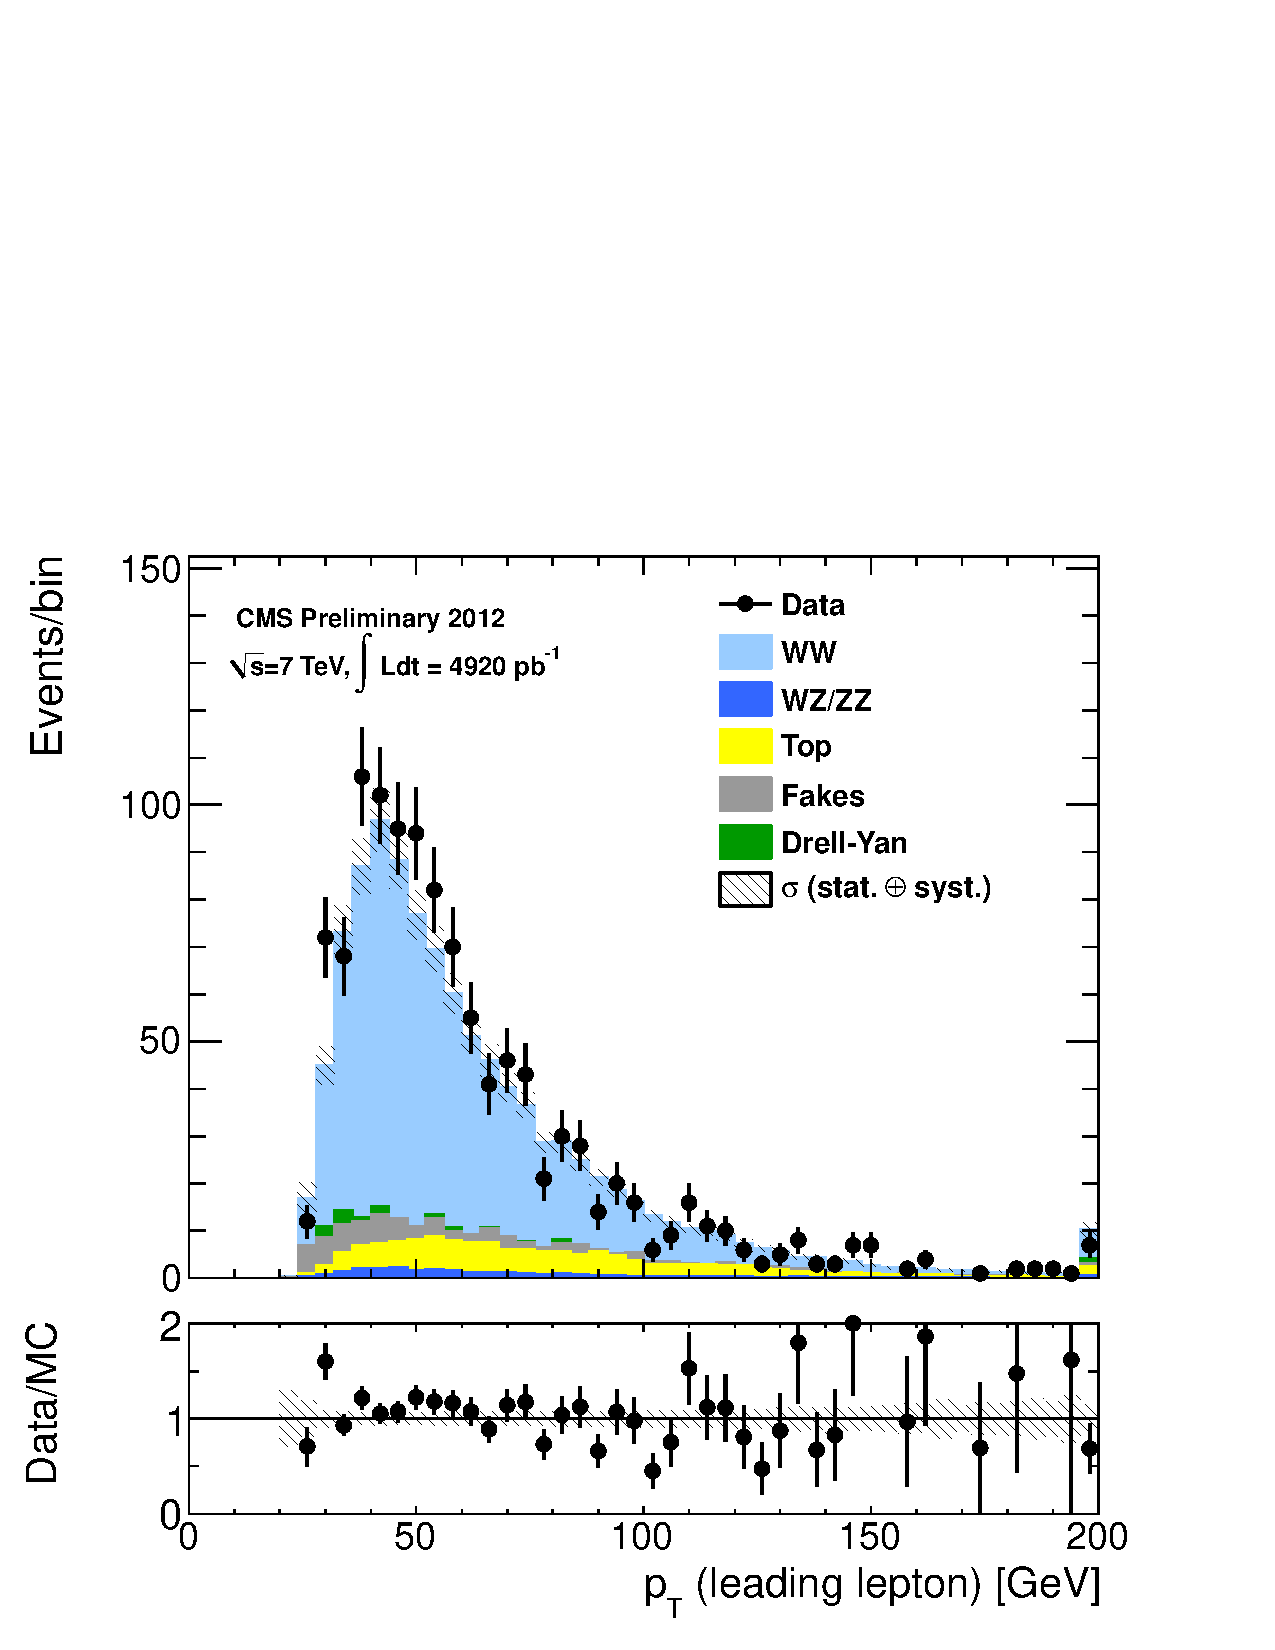
\includegraphics[width=.45\textwidth]{figures/pas_pt1_incl.pdf}}
\subfigure[Log scale]{\label{subfig:pas_pt1_incl_log}
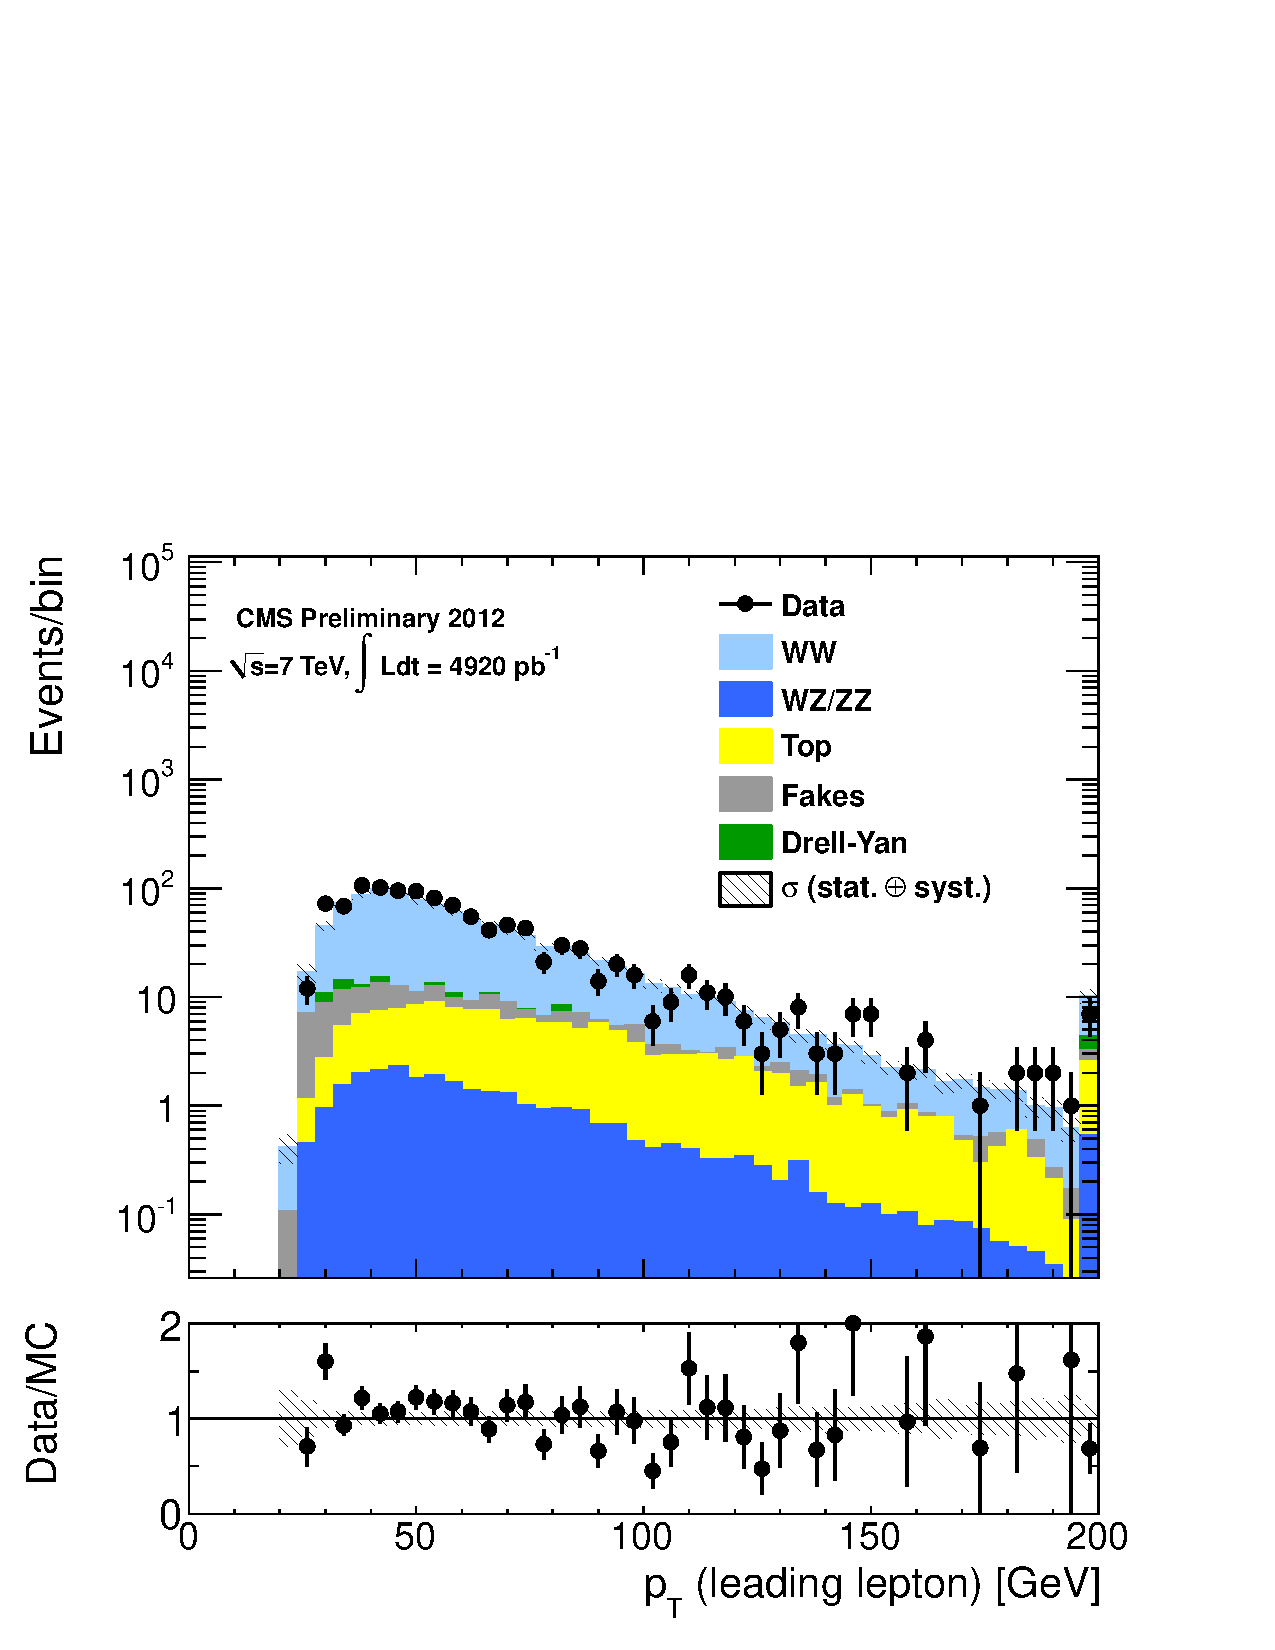
\includegraphics[width=.45\textwidth]{figures/pas_pt1_incl_log.pdf}}
\caption{Leading lepton \pt.}
\label{fig:pas_pt1_incl}
\end{figure}


  
\section{Data Samples}
  \label{sec:datasets}
  %UPDATEME%
The datasets used for this analysis are summarized in Tables.~\ref{tab:DatasetsData} 
and~\ref{tab:DatasetsMC} for data and Monte Carlo, respectively. The total integrated
luminosity is 49 $\pm$ 2 $\ipb$. We used just basic quality requirements, since an official good 
run list (JSON file) was not available. It will be used in future updates.
For Monte Carlo simulation we use madgraph when possible, 
but different generators such as Pythia and Powheg 
are also used. 
%For $gg \to \WW$ a dedicated generator is used. For \wz\ and \zz\
%processes we use Pythia, since MadGraph samples are mixed with $\WW$ in
%a single $VV$ sample, which is difficult to use properly.

%The choice of the Monte Carlo samples depends on the sample
%availability, but in general we tried to be consistent and use a
%single generator - MadGraph. In the case of Drell-Yan, MadGraph samples
%are not adequate to cover the full mass spectrum. The main sample has a 50 $\GeVcc$ 
%minimum dilepton mass requirement, while the other one, covering
%the low mass region, has an additional requirement on extra jet
%activity. 
%We use madgraph when possible, but different generators are used for some samples
%For $gg \to \WW$ a dedicated generator is used. For \wz\ and \zz\
%processes we use Pythia, since MadGraph samples are mixed with $\WW$ in
%a single $VV$ sample, which is difficult to use properly.

%UPDATEME%
\begin{table}[!ht]
\begin{center}
\begin{tabular}{|c|c|}
\hline
 Dataset Description                   &   Dataset Name   \\
\hline
\hline
\multicolumn{2}{|c|}{$H \to \WW$ Signal Selection Samples} \\
\hline
Run2011A MuEl PromptReco            &  /MuEG/Run2011A-PromptReco-v*/AOD   \\
Run2011A DiMuon PromptReco          &  /DoubleMu/Run2011A-PromptReco-v*/AOD   \\
Run2011A SingleMuon PromptReco      &  /SingleMu/Run2011A-PromptReco-v*/AOD   \\
Run2011A DiElectron PromptReco      &  /DoubleElectron/Run2011A-PromptReco-v*/AOD   \\
\hline
\hline
\multicolumn{2}{|c|}{Fake Rate Measurement Samples} \\
\hline
Run2010A Jet  PromptReco            & /Jet/Run2011A-PromptReco-v*/AOD	\\
Run2010B Photon PromptReco          & /Photon/Run2011A-PromptReco-v*/AOD \\
\hline
\end{tabular}
\caption{Summary of data datasets used.\label{tab:DatasetsData}}
\end{center}
\end{table}

\begin{table}[!ht]
\begin{center}
{\footnotesize
\begin{tabular}{|c|c|c|}
\hline
\multicolumn{3}{|c|}{With Pileup: Processed dataset name is always} \\
\multicolumn{3}{|c|}{/Spring11-PU\_S1\_START311\_V1G1-v*/AODSIM} \\
\hline
 Dataset Description                     &   Primary Dataset Name   & cross-section (pb)\\
\hline
qq $\rightarrow WW$                  	 &   /VVJetsTo4L\_TuneD6T\_7TeV-madgraph-tauola                        &  43.0  \\
gg $\rightarrow WW \to 2l 2\nu$          &   /GluGluToWWTo4L\_TuneZ2\_7TeV-gg2ww-pythia6                       &   0.153\\
$\ttbar$                              	 &   /TTJets\_TuneZ2\_7TeV-madgraph-tauola                             & 157.5 \\
$\singletops$                  	 	 &   /TToBLNu\_TuneZ2\_s-channel\_7TeV-madgraph                        &  1.4 \\
$\singletopt$                  	 	 &   /TToBLNu\_TuneZ2\_t-channel\_7TeV-madgraph                        &  20.9 \\
tW                                    	 &   /TToBLNu\_TuneZ2\_tW-channel\_7TeV-madgraph                       &  10.6 \\
Z[20-inf] $\rightarrow ee$	  	 &   /DYToEE\_M-20\_CT10\_TuneZ2\_7TeV-powheg-pythia                   &  1666.0 \\
Z[20-inf] $\rightarrow \mu\mu$        	 &   /DYToMuMu\_M-20\_CT10\_TuneZ2\_7TeV-powheg-pythia                 &  1666.0 \\	       
Z[20-inf] $\rightarrow \tau\tau$  	 &   /DYToTauTau\_M-20\_CT10\_TuneZ2\_7TeV-powheg-pythia-tauola        &  1666.0 \\
Z[10-20]  $\rightarrow ee$	  	 &   /DYToEE\_M-10To20\_CT10\_TuneZ2\_7TeV-powheg-pythia               &  3892.9 \\
Z[10-20]  $\rightarrow \mu\mu$    	 &   /DYToMuMu\_M-10To20\_CT10\_TuneZ2\_7TeV-powheg-pythia             &  3892.9 \\
Z[10-20]  $\rightarrow \tau\tau$  	 &   /DYToTauTau\_M-10To20\_CT10\_TuneZ2\_7TeV-powheg-pythia-tauola    &  3892.9 \\
W/Z+$\gamma$                       	 &   /PhotonVJets\_7TeV-madgraph                                       &  165.0 \\
W $\rightarrow$ $\ell\nu$           	 &   /WJetsToLNu\_TuneZ2\_7TeV-madgraph-tauola                         &  31314.0 \\
WZ                               	 &   /WZtoAnything\_TuneZ2\_7TeV-pythia6-tauola                        &  18.2 \\
ZZ                               	 &   /ZZtoAnything\_TuneZ2\_7TeV-pythia6-tauola                        &   5.9\\
$gg \to H \to WW \to 2\ell2\nu$          &   /GluGluToHToWWTo2L2Nu\_M-*\_7TeV-powheg-pythia6                   & vary \\
$gg \to H \to WW \to \ell\tau2\nu$       &   /GluGluToHToWWTo2L2Nu\_M-*\_7TeV-powheg-pythia6                   & vary \\
$gg \to H \to WW \to 2\tau2\nu$          &   /GluGluToHToWWTo2Tau2Nu\_M-*\_7TeV-powheg-pythia6                 & vary \\
$qqH,~H \to WW \to 2\ell2\nu$            &   /VBF\_HToWWTo2L2Nu\_M-*\_7TeV-powheg-pythia6                      & vary \\
$qqH,~ H \to WW \to \ell\tau2\nu$	 &   /VBF\_HToWWTo2Tau2Nu\_M-*\_7TeV-powheg-pythia6                    & vary \\
$qqH,~H \to WW \to 2\tau2\nu$	         &   /VBF\_HToWWToLNuTauNu\_M-*\_7TeV-powheg-pythia6                   & vary \\
$WH/ZH/\ttbar H,~H\to WW$                &   /WH\_ZH\_TTH\_HToWW\_M-*\_7TeV-pythia6                            & vary \\
\hline
\hline
\end{tabular}
}
\caption{Summary of Monte Carlo datasets used.\label{tab:DatasetsMC}. The cross sections for a SM Higgs boson
is taken from the LHC Higgs cross-section working group~\cite{LHCHiggsCrossSectionWorkingGroup:2011ti}}
\end{center}
\end{table}

Due to details in the implementation of the Powheg calculation, the
resulting Higgs $\pt$ spectrum for $gg \to H$ has a much harder
spectrum compared with the most precise spectrum calculated to NNLO
with resummation to NNLL order, as illustrated in
Figure~\ref{fig:h160ww_pthiggs}(a). Therefore, the proper procedure is
to apply an event-by-event rewighting to the Powheg simulated
events. For the time being we correct the $gg \to H \to \WW$ jet bin
efficiency computed from the Powheg Monte Carlo sample, by a scale
factor which is approximately identical for all Higgs masses. The
scale factors applied to each jet bin in the Powheg simulation are
shown in Figure~\ref{fig:h160ww_pthiggs}(b). The jet definition is 
consitent with the one used in the analysis.

\begin{figure}[!htbp]
\begin{center}
   \subfigure[]{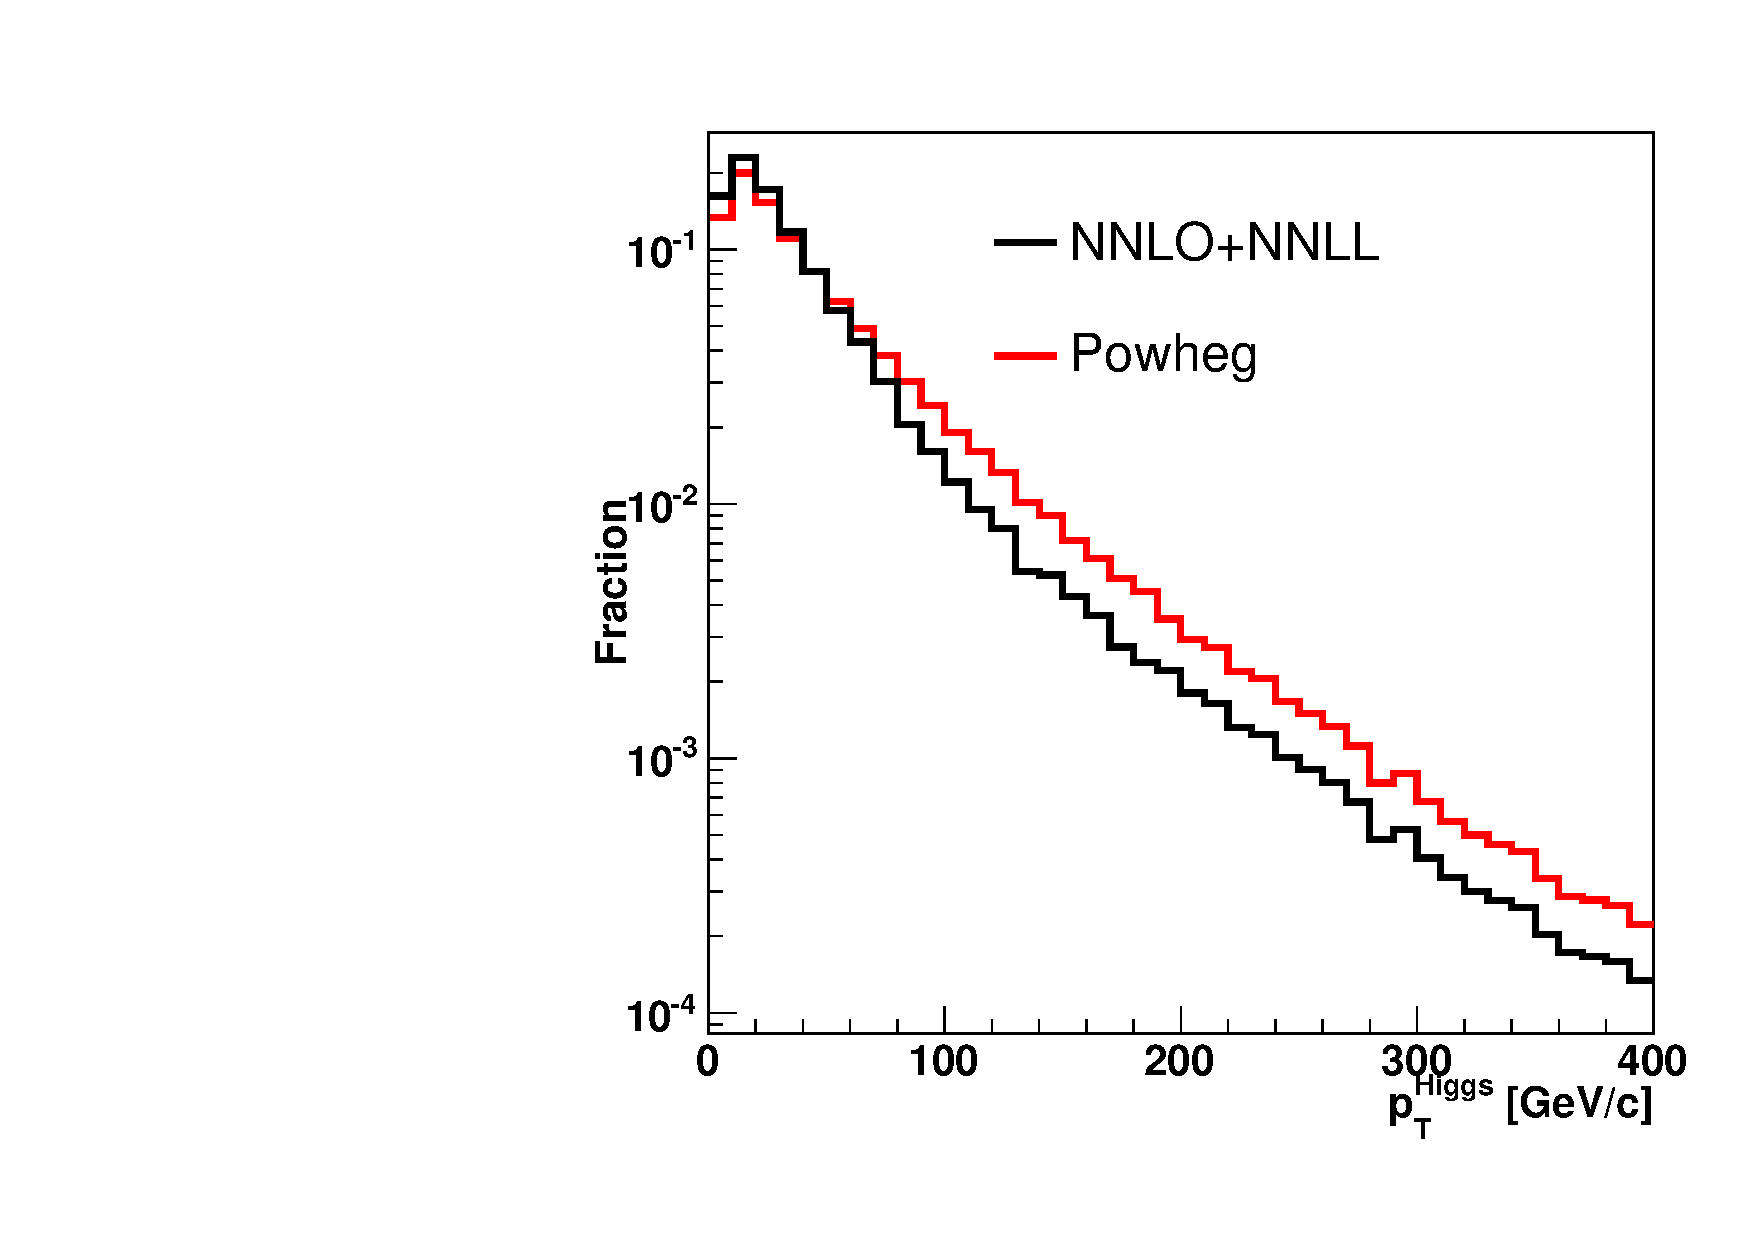
\includegraphics[width=0.49\textwidth]{figures/h160ww_pthiggs.pdf}}
   \subfigure[]{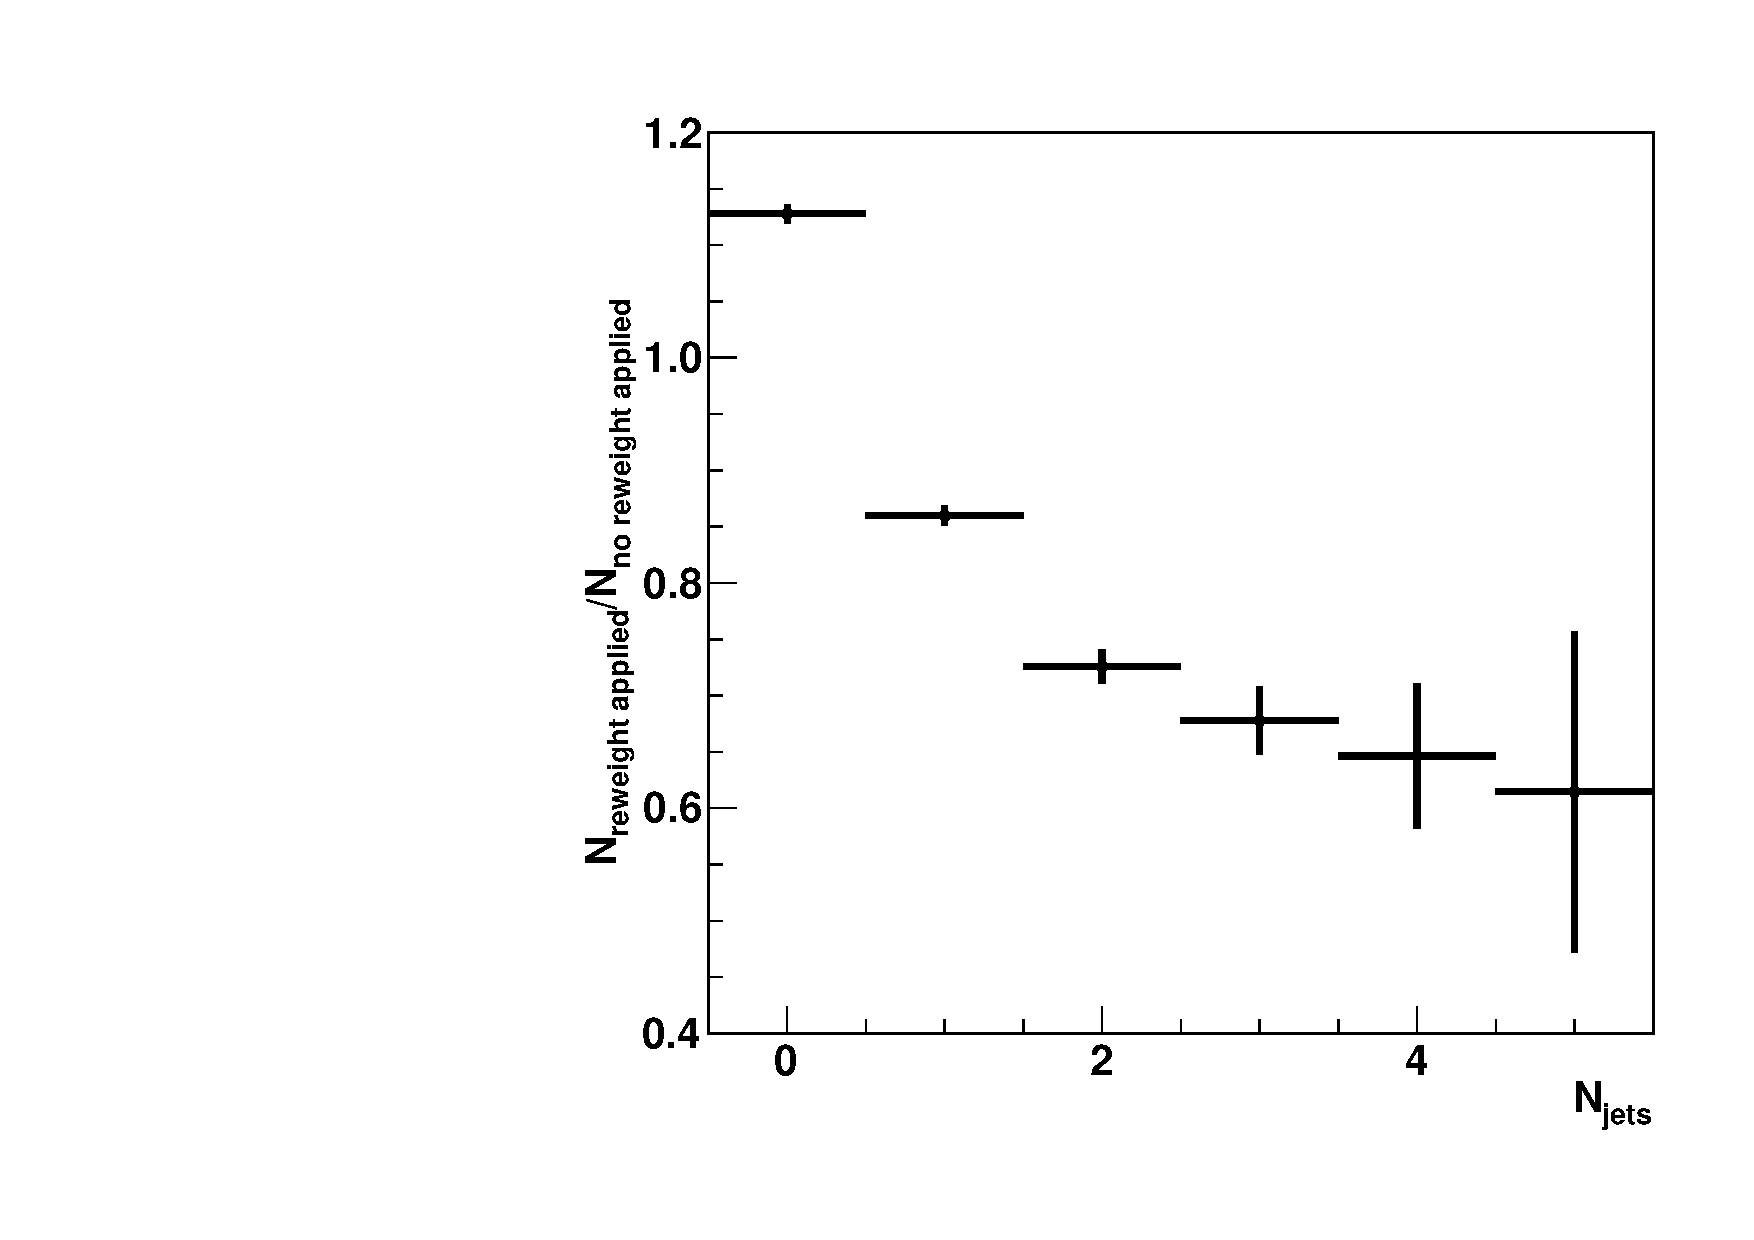
\includegraphics[width=0.49\textwidth]{figures/h160ww_njets_kfactor_ratio.pdf}} 
\caption{(a) Higgs transverse momentum spectrum as predicted by Powheg and the NNLO+NNLL calculation; (b) 
scale factors applied to each jet bin in the Powheg simulation.}
\label{fig:h160ww_pthiggs}
\end{center}
\end{figure}

  
\section{Event Selection}
  \label{sec:selection} 
  To enhance the sensitivity to the Higgs boson signal, two different approaches 
are performed. The first one is a cut-based approach where further requirements 
on a few observables are applied, while the second one makes use of
multivariate techniques. Both of them cover a large Higgs boson mass
($m_{\rm{H}}$) range, and each is separately optimized for different
$m_{\rm{H}}$ hypotheses. The first method is the simplest approach to
be performed on the limited recorded data sample. The second one is
more powerful, since it exploits the information present in the
correlation among the variables. All analyses are further split in 
the corresponding 0-jet, 1-jet and 2-jet bins. Due to the limited 
sensitivity in the 2-jet bin and the little amount of simulated events, 
we decided to have a simple cut-based approach only for now.

  \subsection{Trigger}
    \label{sec:sel_trigger}
    Triggering on Higgs boson decays in the dilepton final state increases 
in difficulty with increasing instantaenous luminosity.
Single lepton triggers can only be sustained with very tight identification and
isolation requirements and large transverse momentum thresholds.
This means that double lepton triggers are the only viable option to maintain
sensitivity to a low mass Higgs boson, where the leptons transverse momentum
can be small.

We use a suite of signal and control triggers designed in the $H \to \WW$ analysis~\cite{HWW2011AN}. 
These dilepton triggers have a high efficiency to collect Higgs boson events
and are sufficiently loose to collect control events to estimate the 
selection efficiencies and with adequate precision.
%We describe the features and motivations for the analysis triggers in Section~\ref{sec:mainTriggers},
%and additional triggers to collect control events in 
%Section~\ref{sec:utilityTriggers}.

%\subsubsection{Analysis Triggers}
%\label{sec:mainTriggers}

The main dielectron triggers, described in Table~\ref{tab:triggers_ee}, require two HLT electron
candidates with loose shower shape and calorimeter isolation requirements on both legs
and a match to a Level-1 seed for the leading leg.
To accomodate the offline selection of $E_{T}>30,20$~GeV for the leading and trailing
electrons, $E_{T}>17,8$~GeV is required at the HLT level.
The main dimuon triggers
require two HLT muon candidates with transverse momentum greater than $7$~$\GeVc$ and
a match to a Level-1 seed is required for both legs.
These are described in Table~\ref{tab:triggers_mm}.

%%%%%%%%%
\begin{table}[!ht]
  \caption{Analysis triggers for the $ee$ final state. 
The identification and isolation requirements are described in Ref.~\cite{HWW2011AN}}.
    \vspace{5pt}
   \label{tab:triggers_ee}
  \begin{center}
 {\small
  \begin{tabular} {l|l|l|c}
\hline
  Dataset & Trigger name & L1 seed & Description\\
  \hline \hline
  \multirow{2}{*}{DoubleElectron} & HLT\_Ele17\_CaloIdL\_CaloIsoVL\_&  L1\_SingleEG12  & $p_T>17,8~\GeVc$ \\
                                  & Ele8\_CaloIdL\_CaloIsoVL &                  & \\

  \multirow{2}{*}{DoubleElectron} & HLT\_Ele17\_CaloIdT\_TrkIdVL\_CaloIsoVL\_TrkIsoVL\_ &  L1\_SingleEG12  & $p_T>17,8~\GeVc$ \\
                                  & Ele8\_CaloIdT\_TrkIdVL\_CaloIsoVL\_TrkIsoVL &                  & \\
  \hline
  \end{tabular}
}
  \end{center}
\end{table}
%%%%%%%%%

%%%%%%%%%
\begin{table}[!ht]
  \caption{Analysis triggers for the $\mu\mu$ final state. Triggers marked (*) are also used for efficiency studies.}
    \vspace{5pt}
   \label{tab:triggers_mm}
  \begin{center}
 {\small
  \begin{tabular} {l|l|l|c}
\hline
  Dataset & Trigger name & L1 seed & Description\\
  \hline \hline
  DoubleMu & HLT\_DoubleMu6 & L1\_DoubleMu3  & $p_T>6,6~\GeVc$\\
  DoubleMu & HLT\_DoubleMu7 & L1\_DoubleMu3  & $p_T>7,7~\GeVc$ \\
  DoubleMu & HLT\_Mu13\_Mu8 & L1\_DoubleMu3  & $p_T>13,8~\GeVc$ \\
  DoubleMu & HLT\_Mu17\_Mu8 & L1\_DoubleMu3  & $p_T>17,8~\GeVc$ \\
  \hline
  \end{tabular}
}
  \end{center}
\end{table}
%%%%%%%%%

%%%%%
\begin{table}[!ht]
  \caption{Single lepton triggers to recover lost efficiency. These trigges are also used for efficiency studies.
The identification and isolation requirements for electrons are described in Table~\ref{tab:HLTElectronCuts}.}
    \vspace{5pt}
   \label{tab:triggers_single}
  \begin{center}
 {\small
  \begin{tabular} {l|l|l|c}
\hline
  Dataset & Trigger name & L1 seed & Description\\
  \hline \hline
  SingleEle & HLT\_Ele27\_CaloIdVT\_CaloIsoT\_TrkIdT\_TrkIsoT & L1\_SingleEG15  & $p_T>27~\GeVc$ \\
  \hline \hline
  SingleMu & HLT\_IsoMu12   & L1\_SingleMu7  & $p_T>12~\GeVc$ \\
  SingleMu & HLT\_IsoMu17   & L1\_SingleMu10 & $p_T>17~\GeVc$ \\
  SingleMu & HLT\_Mu15      & L1\_SingleMu10 & $p_T>15~\GeVc$ \\
  \hline 
  \end{tabular}
}
  \end{center}
\end{table}
%%%%%


%\subsubsection{Utility Triggers}
%\label{sec:utilityTriggers}

%We now describe additional triggers that are introduced to collect control or
%calibration events not covered by the main analysis triggers.

To estimate the non-$Z$ dilepton backgrounds, where the selected dileptons are 
not from the $Z$ details, we need to use the events collected in the $e\mu$ final sates. 
In the electron-muon channel we use two complementary triggers, which require
both muon and electron HLT candidates.
These are summarised in Table~\ref{tab:triggers_em}.
Finally, to recover any residual inefficiency,
we also allow events that passed only the single electron
or single isolated muon triggers summarised in Table~\ref{tab:triggers_single}.

%%%%%
\begin{table}[!ht]
  \caption{Analysis triggers for the $e\mu$ final state.
The identification and isolation requirements for electrons are described in Ref.~\cite{HWW2011AN}.}
    \vspace{5pt}
   \label{tab:triggers_em}
  \begin{center}
 {\small
  \begin{tabular} {l|l|l|c}
\hline
  Dataset & Trigger name & L1 seed & Description\\
  \hline \hline
  MuEG & HLT\_Mu17\_Ele8\_CaloIdL & L1\_Mu3\_EG5 & $p_T>17,8~\GeVc$ \\
  MuEG & HLT\_Mu8\_Ele17\_CaloIdL & L1\_Mu3\_EG5 & $p_T>8,17~\GeVc$ \\
 \hline
  \end{tabular}
}
  \end{center}
\end{table}
%%%%%

Because the main dielectron analysis triggers make requirements on
both legs, events collected with those triggers cannot be used to measure
efficiencies without introducing unacceptable bias.
Thus, to measure the electron selection and trigger efficiency
we introduce two specialised tag and probe triggers designed to maximize
the number of useful \dyll~events, % for both low and high $p_{T}$ electrons,
while keeping the total trigger rate at a reasonable level. 
%The tag and probe method is described later in Section~\ref{sec:efficiency}.

%The first trigger probes low $p_T$ electrons and applies very tight identification 
%and isolation requirements on the tag leg to reduce the background rate.
%The second trigger probes higher $p_{T}$ electrons.
%Both triggers are described in Table~\ref{tab:triggers_util} and labeled "eff".

Another set of specialised triggers are used to record events
enriched in fake electrons and muons for the measurement of jet induced backgrounds.
This is done using the fake rate method, which is described in detail in ref.~\ref{sec:HWW2011AN}. 
{\bf \fixme{} Add the photon jet triggers..}

  \subsection{Primary Vertex Reconstruction}
    \label{sec:sel_pv}
    Primary vertices are reconstructed using the so-called Deterministic Annealing (DA) 
clustering of tracks~\cite{PVDA}. Reconstructed primary vertices are required to have a
$z$ position within 24~cm of the nominal detector center and a radial position within 
2~cm of the beamspot. There must also be greater than four degrees of freedom in
the fitted vertex. From the set of primary vertices in the event passing these
selection cuts, the vertex with the largest summed squared-$\pt$ of the associated
tracks is chosen as the event primary vertex. Reconstructed leptons will be required 
to have small impact parameters with respect to this vertex.

Due to the fast evolution of the LHC machine, with a rapid rise in the
instantaneous luminosity, the data taking conditions have changed
rapidly.  In particular it is difficult to exactly reproduce the
number of overlapping events (i.e. pileup) between data and
simulation, and thus there will be differences in the number of
reconstructed primary vertices. 
To make sure the simulation reproduces the data, we reweight the number of
primary verteces in the simulation to match the distribution observed in the 
data, after requiring that the event has two leptons passing offline
lepton selection.

  \subsection{Muon Selection} 
    \label{sec:sel_muons}
   Muons in CMS are reconstructed as either $StandAloneMuons$ (track
in the muon detector with low momentum resolution), $GlobalMuons$
(outside-in approach seeded by a $StandAloneMuon$ with a global fit
using hits in the muon, silicon strip and pixel 
detectors) and $TrackerMuons$ (inside-out approach seeded by an offline 
silicon strip track, using the muon detector only for muon identification 
without refitting the track). Most good quality muons are reconstructed as 
all three types at the same time and the momentum resolution is dominated by the inner
tracker system up to about 200~$\GeVc$ in transverse momentum. Details about the
optimization at low $\pt$ are given in Appendix~\ref{app:mus}. The specific
requirements to select good prompt isolated muons are the following:
\begin{itemize}
\item the muon must be found by both the global and tracker muon algorithms;
\item the global muon must have at least one good muon hit;
\item the tracker muon must have at least two matches to muon segments in 
      different muon stations;
\item more than 10 hits in the inner tracker;
\item at least one pixel hit;
\item $\chi^2/{\mathrm{ndof}} < 10$ on a global fit;
\item impact parameter in the transverse plane $|d_{0}| < 0.02~(0.01)$~cm for
      muons with $\pt$ greater (smaller) than 20 $\GeVc$,
      calculated with respect to the primary vertex;
\item longitudinal impact parameter $|d_{z}| <0.2$~cm,
      calculated with respect to the primary vertex;
\item pseudorapidity $|\eta|$ must be smaller than 2.4;
\item relative \pt\ resolution is better than 10\%.
\end{itemize}

Furthermore, the particle flow candidate-based isolation variable is 
used to reduce the contamination from the non-isolated muons originating from
jets. 

\begin{itemize}
\item $\rm{Iso}_{PF}$: defined as the scalar sum of the \pt\ of the 
    particle flow candidates satisfying the following requirements:
    \begin{itemize}
    \item $\Delta R~<~0.3$ to the muon in the $\eta \times \phi$ plane,
    \item $|d_{z}(\mathrm{PF Candidate}) - d_{z}(\mathrm{muon})| < 0.1$~cm, if the PF candidate is charged,
    \item \pt $>1.0$ GeV, if the PF candidate is classified as a neutral hadron or a photon.
    \end{itemize}
\end{itemize}

We require $\frac{\rm{Iso}_{PF}}{\pt}~<~0.13~(0.06)$ for muons in the barrel 
with $\pt$ greater (smaller) than 20 $\GeVc$. For muons in the endcap, we
require $\frac{\rm{Iso}_{PF}}{\pt}~<~0.09~(0.05)$ for muons with $\pt$ 
greater (smaller) than 20 $\GeVc$. Further details of the choice of
the isolation requirement is documented in Appendix \ref{app:pfIsoStudy}.


  \subsection{Electron Selection} 
    \label{sec:sel_electrons}
    We identify electrons using a multivariate approach optimized 
for this analysis~\cite{MVAElId}. In addition, we require some minimal 
requirements to make sure the electron candidate is as tight as the 
trigger selection:

\begin{itemize}
  \item $p_T>10$~GeV and $|\eta| < 2.5$
  \item $\sigma_{i\eta i\eta} < 0.01/0.03$ (barrel/endcap)
  \item $|\Delta\phi_{in}| < 0.15/0.10$
  \item $|\Delta\eta_{in}| < 0.007/0.009$
  \item $H/E< 0.12/0.10$ (barrel/endcap)
  \item $\frac{\sum_{\rm trk}\Et}{\pt^{\rm ele}}<0.2$
  \item $\frac{\sum_{\rm ECAL}\Et}{\pt^{\rm ele}}<0.2$
  \item $\frac{\sum_{\rm HCAL}\Et}{\pt^{\rm ele}}<0.2$
\end{itemize}

Isolation requirements are then imposed by computing the particle flow isolation,
defined as the scalar sum of the \pt\ of the particle flow candidates satisfying 
the following requirements:

\begin{itemize}
\item $\Delta R~<~0.4$ to the electron in the $\eta \times \phi$ plane,
\item for neutral hadron PF candidates, require that it is outside the footprint veto region of $\Delta R~<~0.07$,
\item for photon and electron PF candidates, require that it is outside the footprint veto region of $|\Delta\eta|<0.025$,
\item $|d_{z}(\mathrm{PF~candidate}) - d_{z}(\mathrm{muon})| < 0.1$~cm, if the PF candidate is charged,
\item \pt $>1.0$ GeV, if the PF candidate is classified as a neutral hadron or a photon.
\end{itemize}

We require $\frac{\rm{Iso}_{PF}}{\pt}~<~0.13~(0.09)$ for electrons in the barrel (endcap).

In order to veto fake electrons from converted photons, 
we look for a reconstructed conversion vertex where one of the two tracks 
is compatible with the electron~\cite{ConversionNote}.
The vertex fit probability is required to be $>10^{-6}$.
We then require that there are no missing expected missing hits forming the electron track~\cite{ConversionNote},~\cite{NExpHits}. 
Finally to reduce fake electrons from non-prompt sources,
we require the transverse and longitudinal impact parameters with
respect to the primary vertex to be less than $0.02$ and $0.1$~cm respectively.

  \subsection{Missing Energy} 
    \label{sec:sel_met}
    
The missing transverse energy is used to reject background events
where there is no natural source of missing energy, like in Drell-Yan and
QCD events. In the $\dytt$ process there is a large difference in the masses of 
$\tau$ and $\Z$. The taus are produced with large boost and their decay products, including 
neutrinos, are aligned with the leptons. Therefore a transverse component 
of missing energy with respect to the leptons is a better measure of true 
missing energy in the event, not originating from $\tau$ decay. 
To reject such background events with a small opening angle
between \met\ and one of the leptons, we used the projected \met~\cite{HWW2010} for 
event selection, defined as:
\begin{equation}
\text{with } \Delta\phi_{min} =  min(\Delta\phi(\ell_1,\met),\Delta\phi(\ell_2,\met))\\
\end{equation}
\begin{equation}
= 
\begin{cases} \met & \text{if $\Delta\phi_{min}>\frac{\pi}{2}$,}
\\
\met\sin(\Delta\phi_{min}) & \text{if $\Delta\phi_{min}<\frac{\pi}{2}$}
\end{cases}
\end{equation}
where $\Delta\phi(\ell_i,\met)$ is the angle between \met\ and lepton
 $i$ in the transverse plane.

In the presence of high multiple-interactions (pile-up), the instrumental \met\ tail in 
$\dyll$ events increases significantly. 
Figure~\ref{fig:met_pu} shows the projected particle-flow MET~\cite{PFMET} in the 
events with low ($<$5) and high ($>5$) primary vertices in both $\dyll$ data and MC. 
The $\dyll$ events in data are selected by requiring the dilepton invariant mass 
within 15 $\GeVcc$ of the $Z$ mass. 
This leads to a large increase of the background contribution in the signal region, as shown in 
Figure~\ref{fig:meteff_pu}. 
%This causes a sharp increase in the efficiency for $\dyll$ events to pass a given \met\ 
%requirement as the number of pile-up interactions increases. 
%To improve the robustness of the \met\ performance in the presence of pile-up, 
To improve the signal over background performance of \met\ selections in the presence of pile-up, 
we have developed a novel \met\ algorithm referred to as ``trk-MET''~\cite{FIXME}, constructed from 
charged particles consistent with originating from the primary vertex. 
The event $\met$ trk-MET is defined as 
\begin{equation}
\text{trk-MET} \equiv -\overrightarrow{p_T}(l_1) - \overrightarrow{p_T}(l_2) - \sum_i{\overrightarrow{p_T}(i)}, \\
\label{eq:trkmet}
\end{equation}
where $\overrightarrow{p_T}(l_1)$ and $\overrightarrow{p_T}(l_2)$ are the transverse momentum vectors of the two 
leptons passing the lepton selections described in Section~\ref{sec:sel_muons}-\ref{sec:sel_electrons}, 
and $\overrightarrow{p_T}(i)$ represent the tranverse momentum vectors of the charged PFCandidates satisfying the following requirements:
%%%%%%%%%%%%%%%%%%%%%%%%%%
\begin{itemize}
\item the track matched to PFCandidate has $\Delta z < 0.1$~cm with respect to the signal PV, which is the 
closest PV to the track in $\Delta z$;
\item the track has $\Delta R > 0.1$ with respect to both leptons, to avoid double-counting of the leptons.
\end{itemize}
%%%%%%%%%%%%%%%%%%%%%%%%%%

Comparing to the projected PFMet, we observed that the projected trk-MET has 
a larger tail in $\dyll$ background events~\cite{FIXME}. 
However these two \met\ values are weakly-correlated in $\dyll$ backgrounds with no geninue $\met$, and 
strongly correlated for the signal processes with geninue $\met$, as shown in Figure~\ref{fig:met_scatter}. 
Therefore the signal over background ratio is optimized if we select the events 
based on the mininum of these two projected $\met$ values, $\text{min-MET} \equiv min(\text{proj}_\text{trk-MET}, \text{proj}_\text{PFMET})$. 


The selection requirements are different between \ee{}/\mm{}
and \emu{} final states since Drell-Yan mostly contributes to \ee\
and \mm\ channels. The selection requirements are:
\begin{itemize}
\item projected $\met>20~\GeV$ for \emu{}
\item projected $\met>35~\GeV$ for \ee{} and \mm{} 
\end{itemize}
The selection efficiencies for the signal ($\hww$ at $m_{H}=130$ GeV) and background ($\dyll$) 
events are shown in Figure~\ref{fig:met_eff} as a function of $\met$ requirements. 
Using min-MET we see that the signal selection efficiency improves while the background selection efficiency reduces significantly 
compared to the values obtained using projected PFMet. 
In addition, the background selection efficiency dependendence on the 
number of primary vertices is largely reduced as well using min-MET. 


%%%%%%%%%%%%%%%%%%%%%%%%%%%%%%%%%%%%%%%%%%%
\begin{figure}[hbt]
\begin{center}
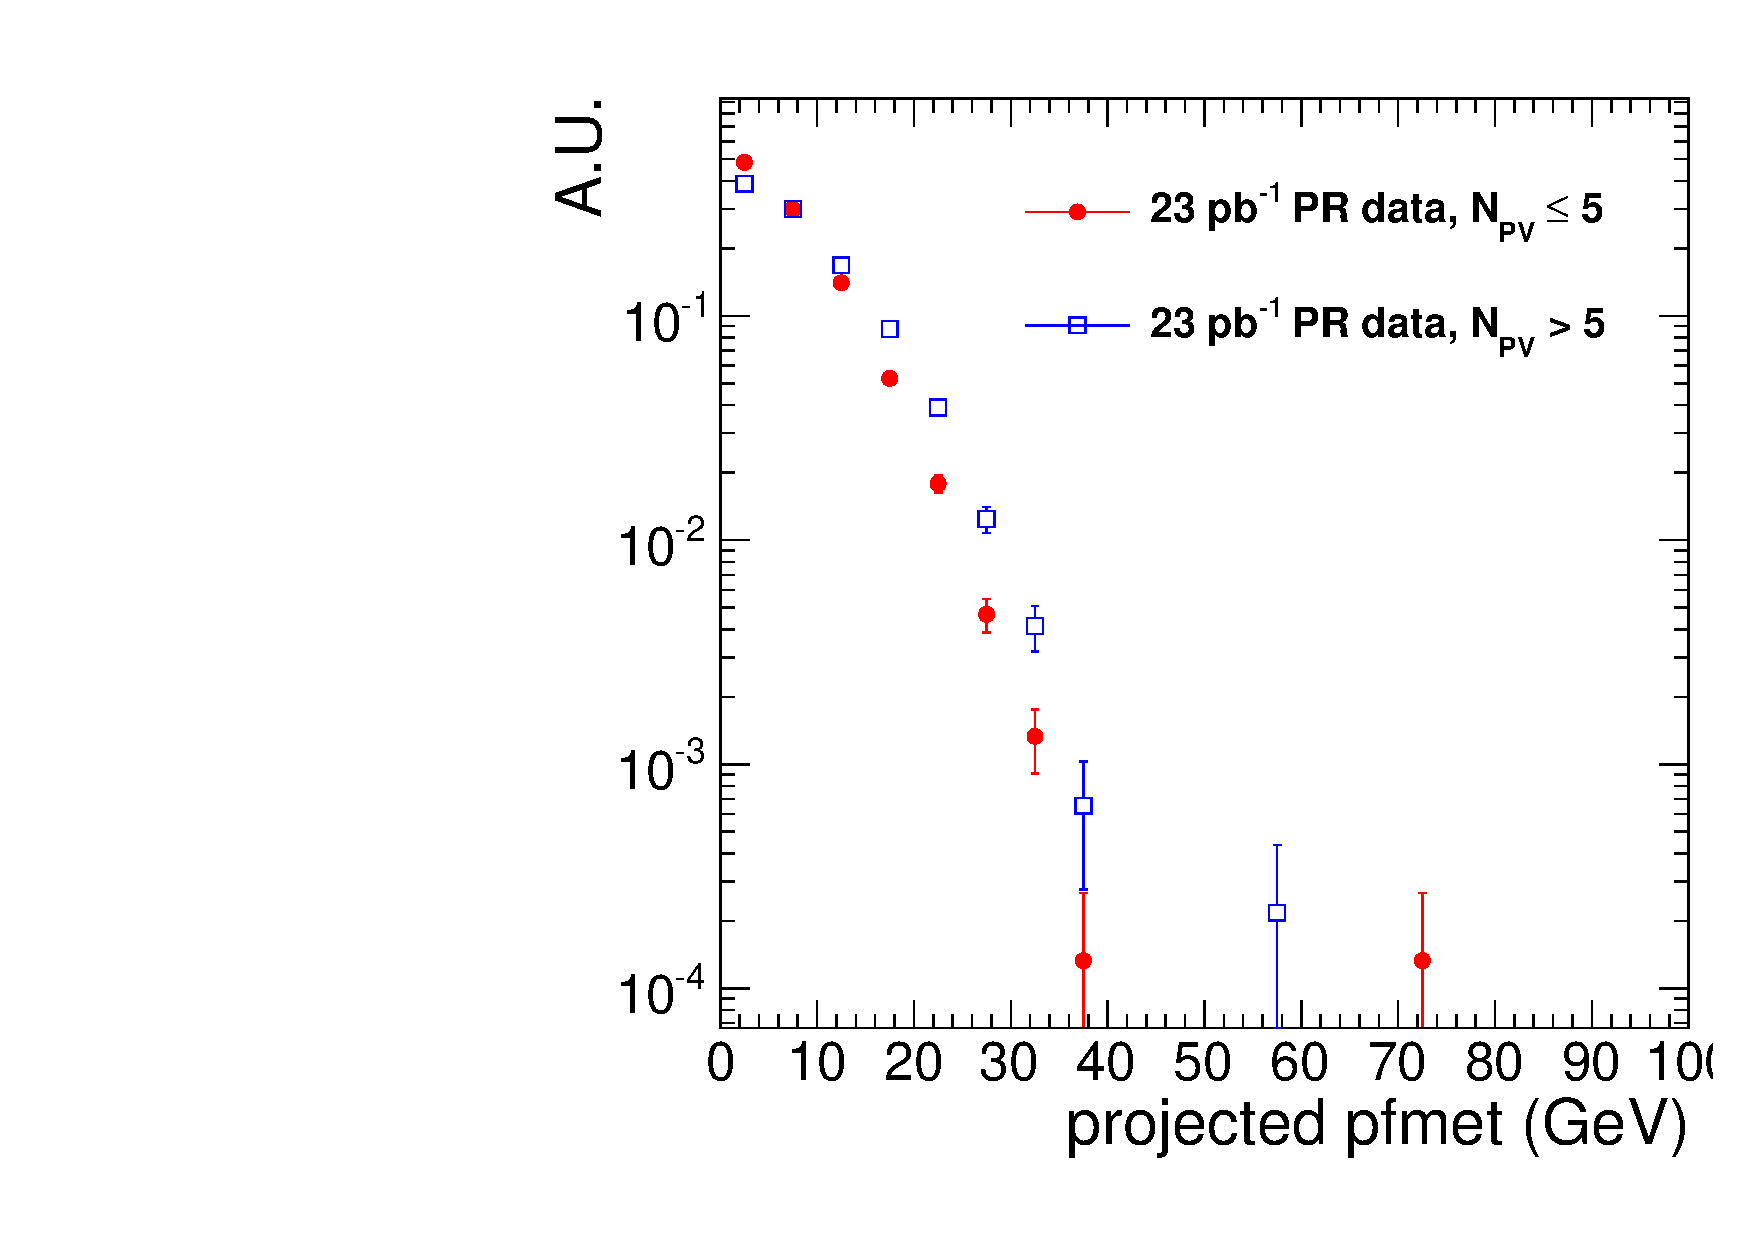
\includegraphics[width=0.4\linewidth]{figures/pfmet_data.pdf} 
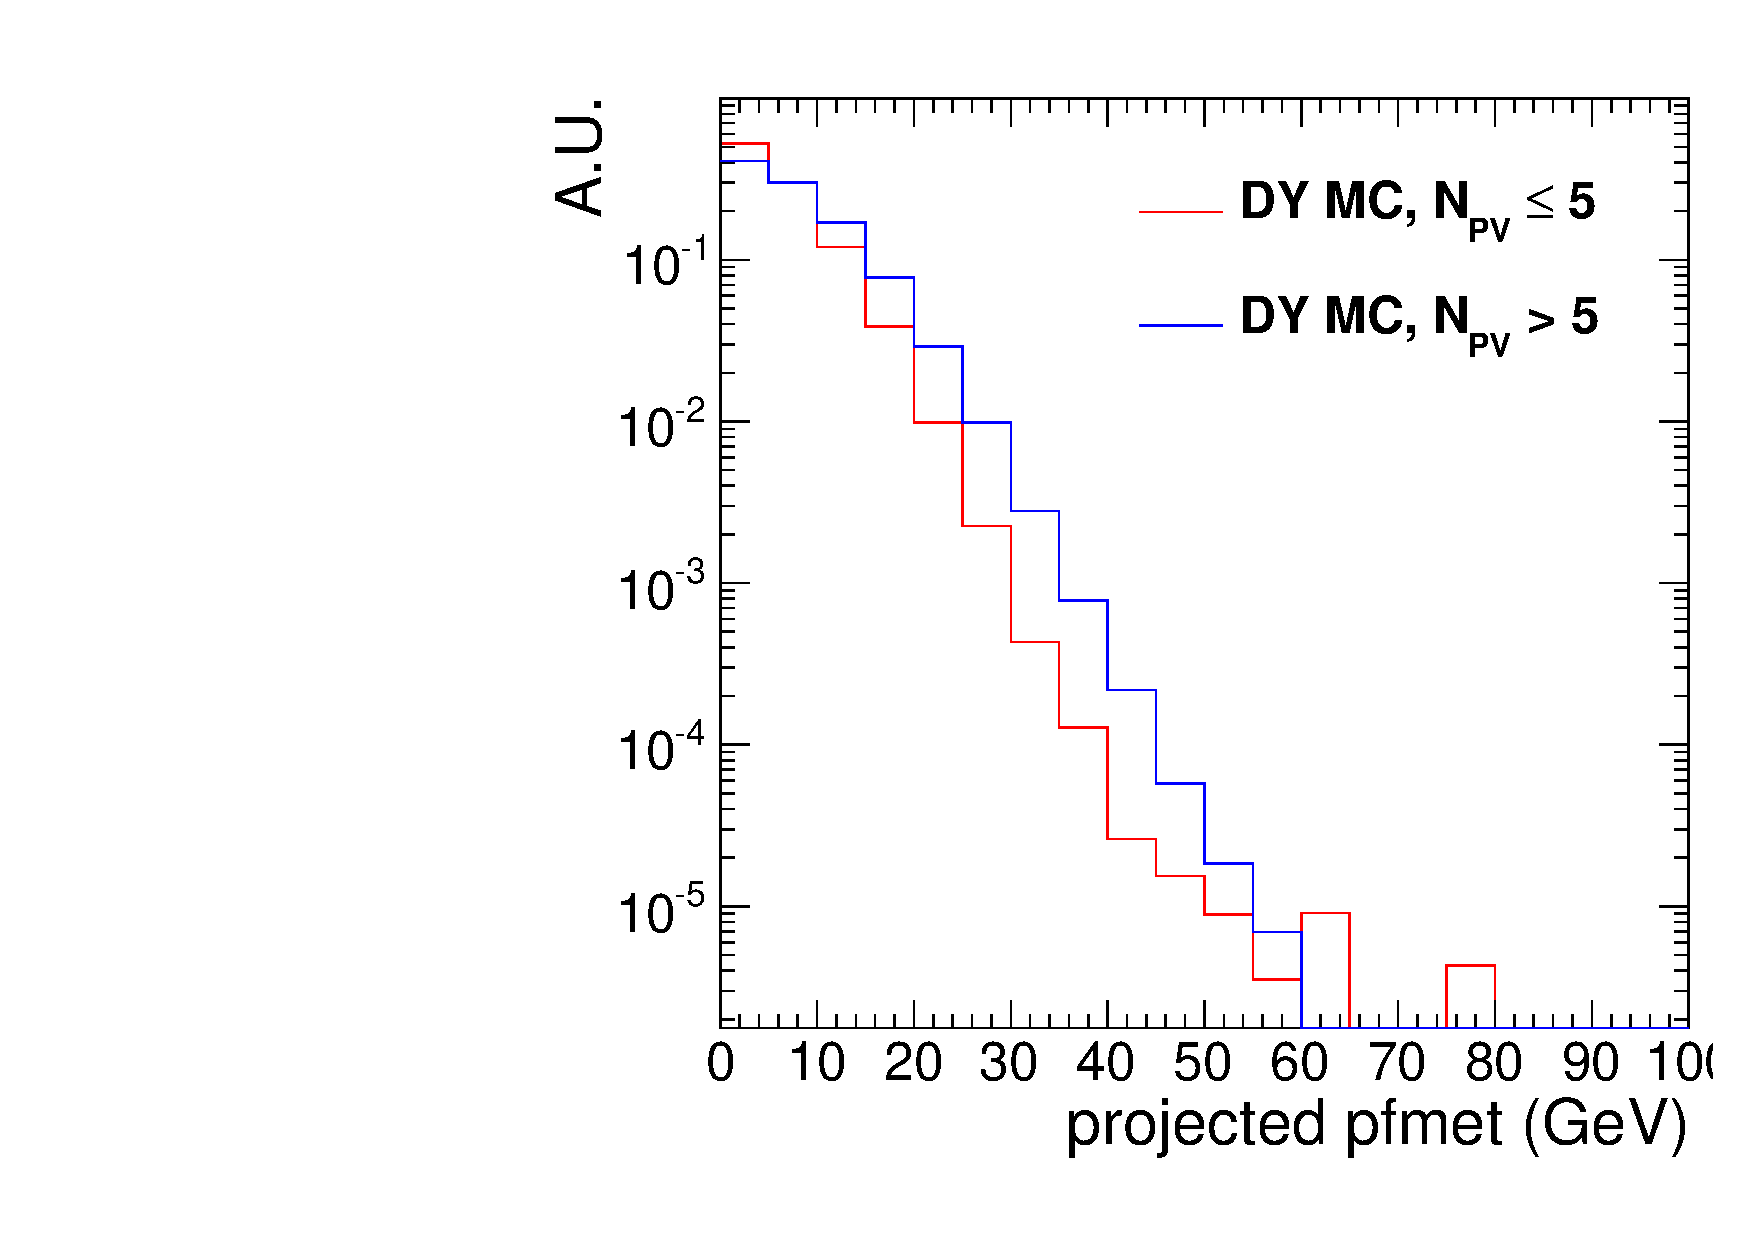
\includegraphics[width=0.4\linewidth]{figures/pfmet_dymc.pdf}
%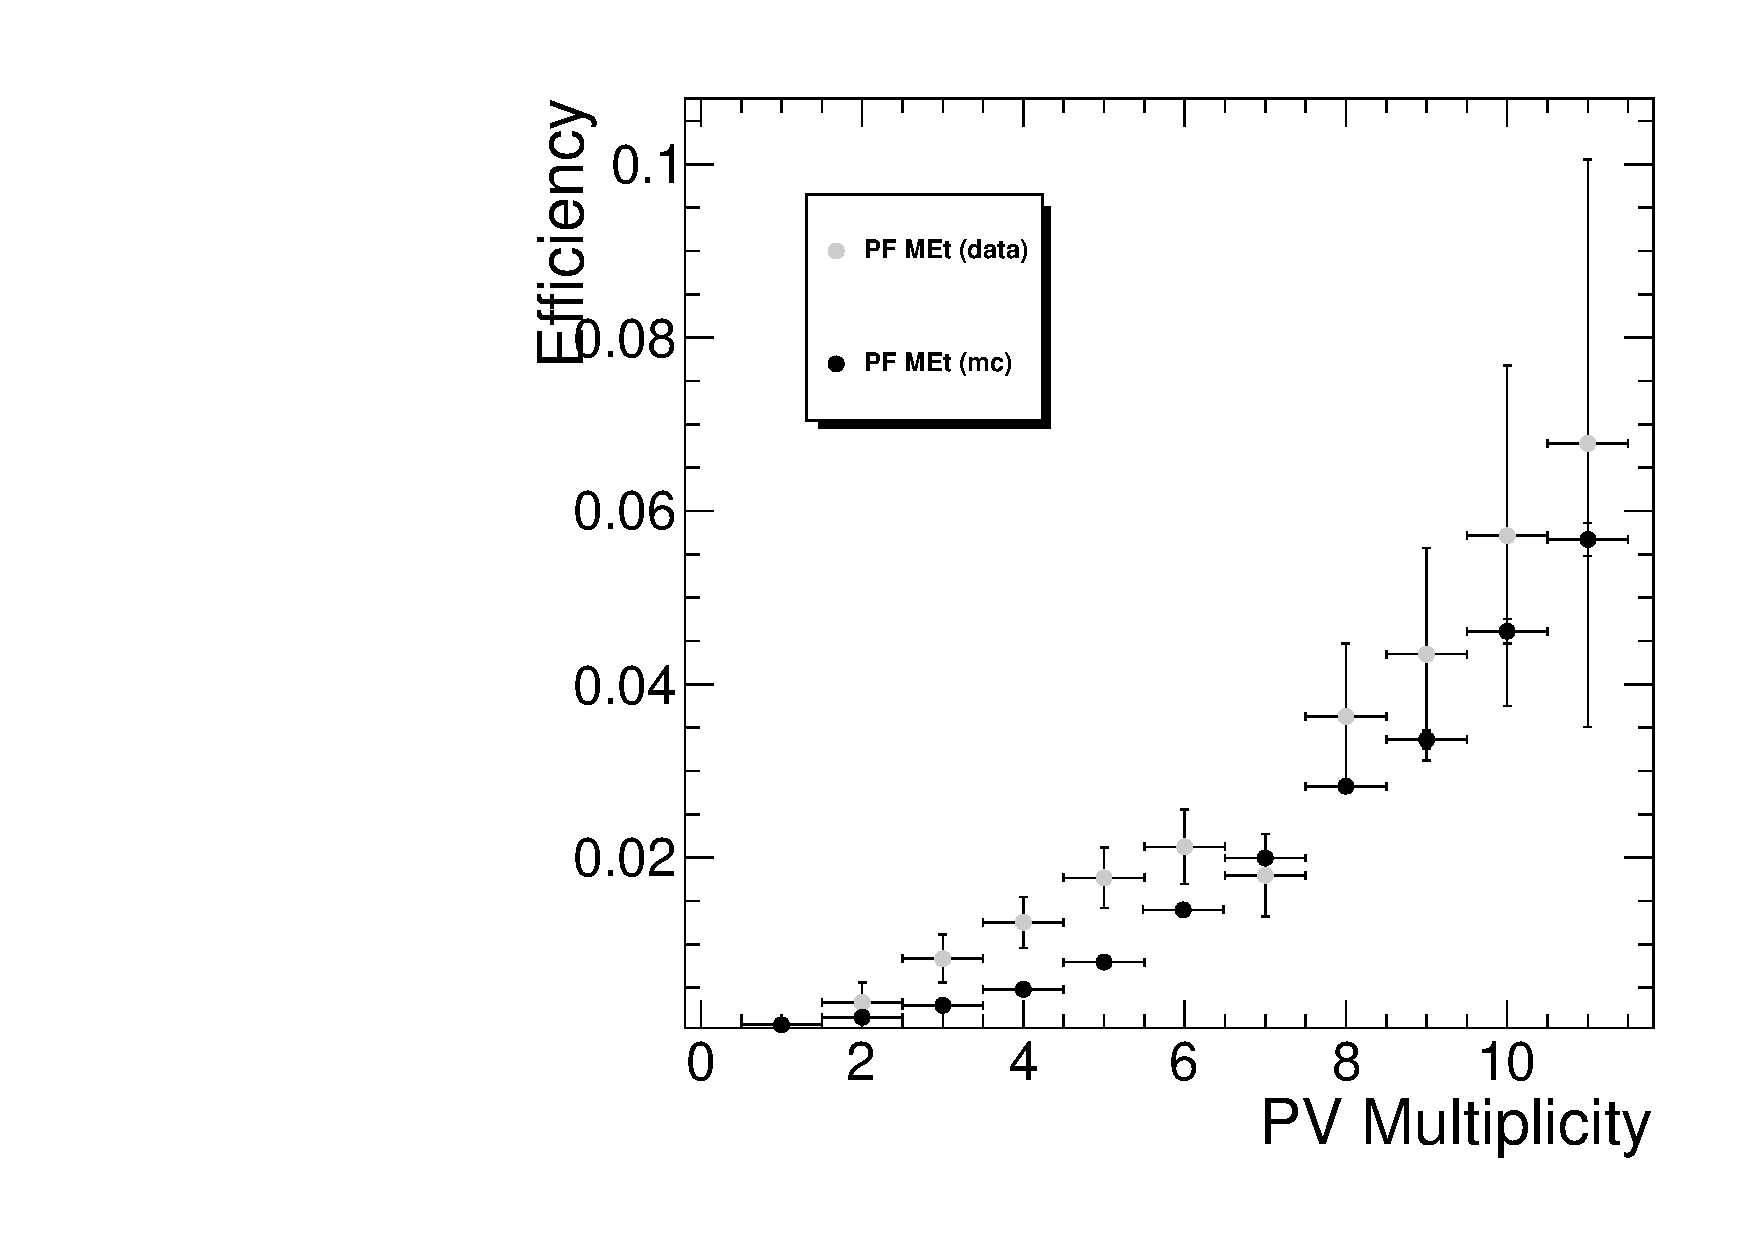
\includegraphics[width=0.3\linewidth]{figures/pfmet_Eff30.pdf} 
\caption{\label{fig:met_pu}\protect Distributions of projected PFMet in data (left) and $\dyll$ MC (center) 
overlayed for low pile-up and high pile-up. The efficiency to satisfy the requirement pfmet$>30$~GeV as a function
of the number of reconstructed vertices in $\dyll$ data and MC.}
\end{center}
%\end{figure}
%%%%%%%%%%%%%%%%%%%%%%%%%%%%%%%%%%%%%%%%%%%
%%%%%%%%%%%%%%%%%%%%%%%%%%%%%%%%%%%%%%%%%%%
%\begin{figure}[hbt]
\begin{center}
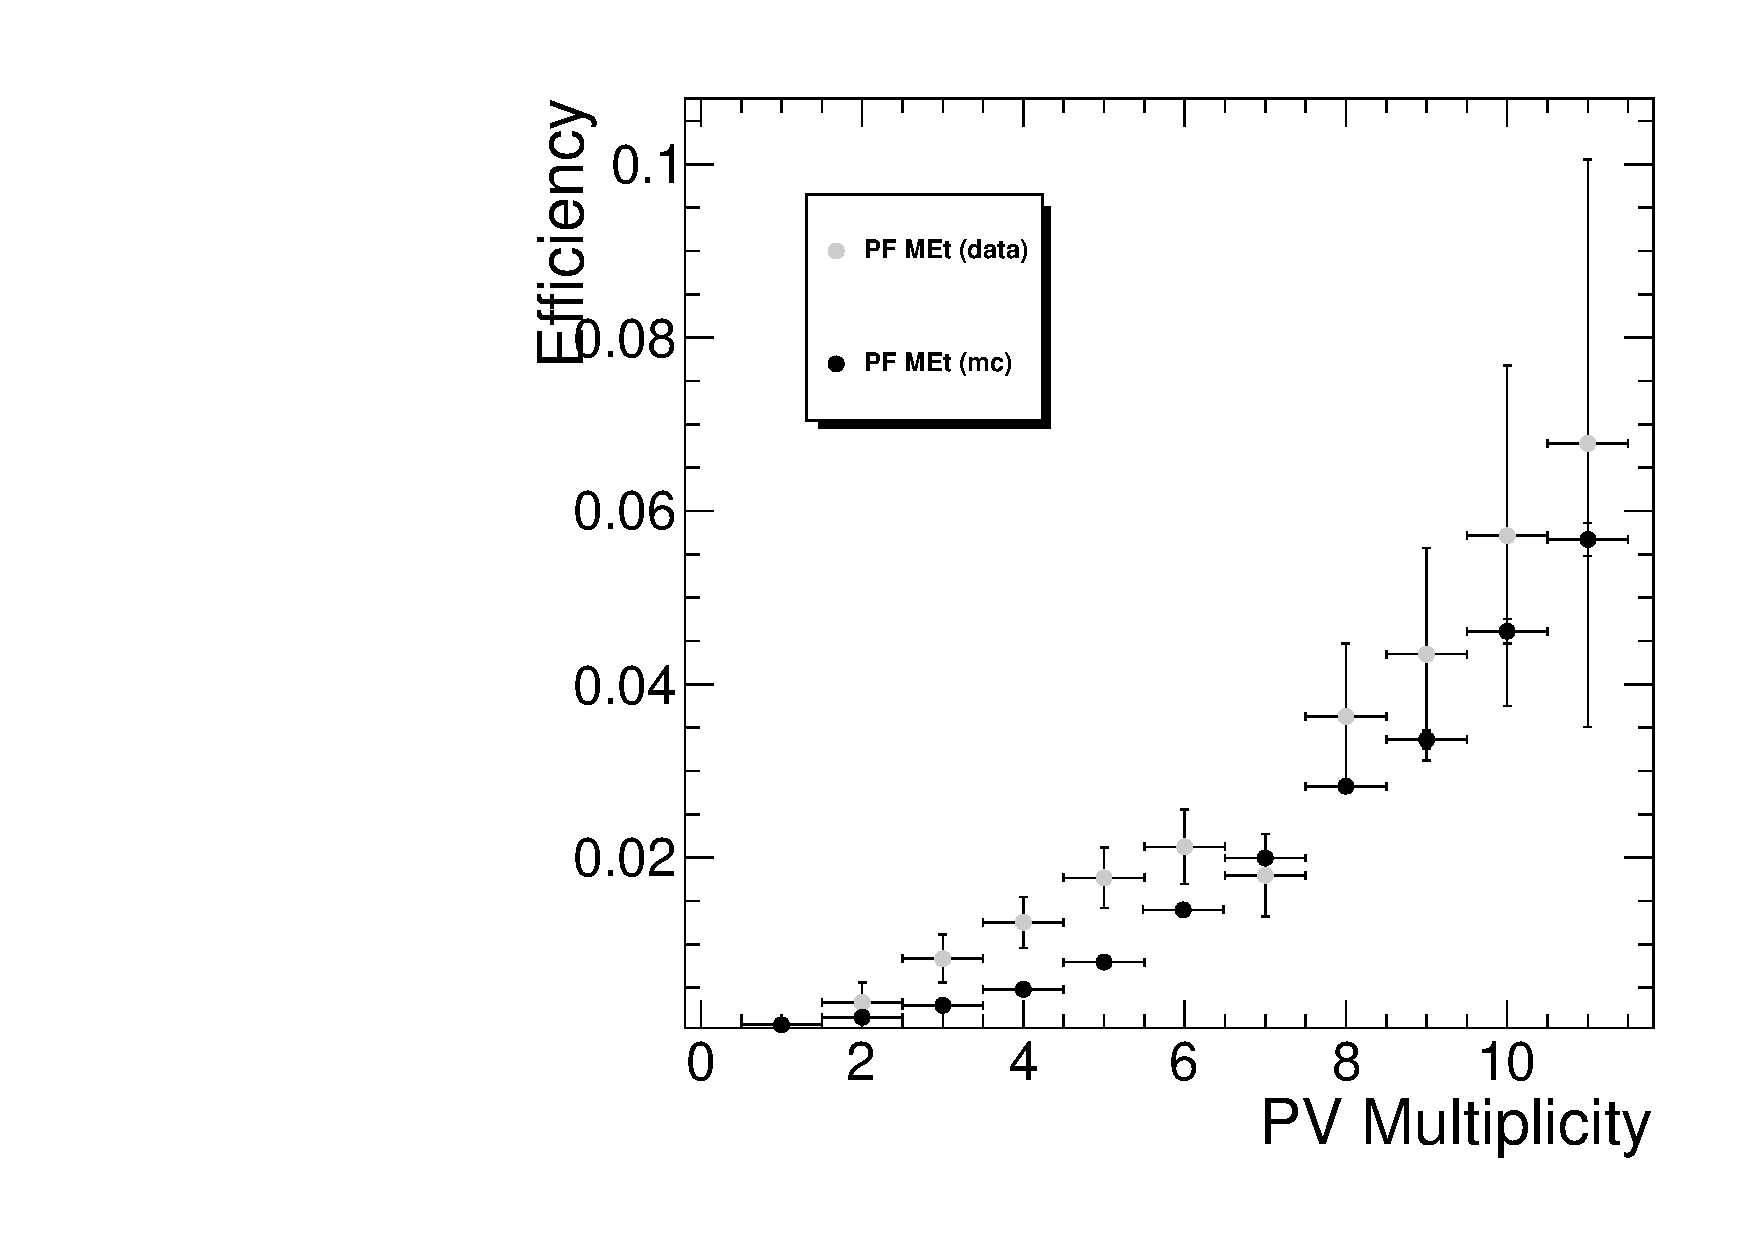
\includegraphics[width=0.5\linewidth]{figures/pfmet_Eff30.pdf} 
\caption{\label{fig:meteff_pu}\protect The efficiency to satisfy the requirement pfmet$>30$~GeV as a function
of the number of reconstructed vertices in $\dyll$ data and MC.}
\end{center}
\end{figure}
%%%%%%%%%%%%%%%%%%%%%%%%%%%%%%%%%%%%%%%%%%%

%%%%%%%%%%%%%%%%%%%%%%%%%%%%%%%%%%%%%%%%%%%
\begin{figure}[hbt]
\begin{center}
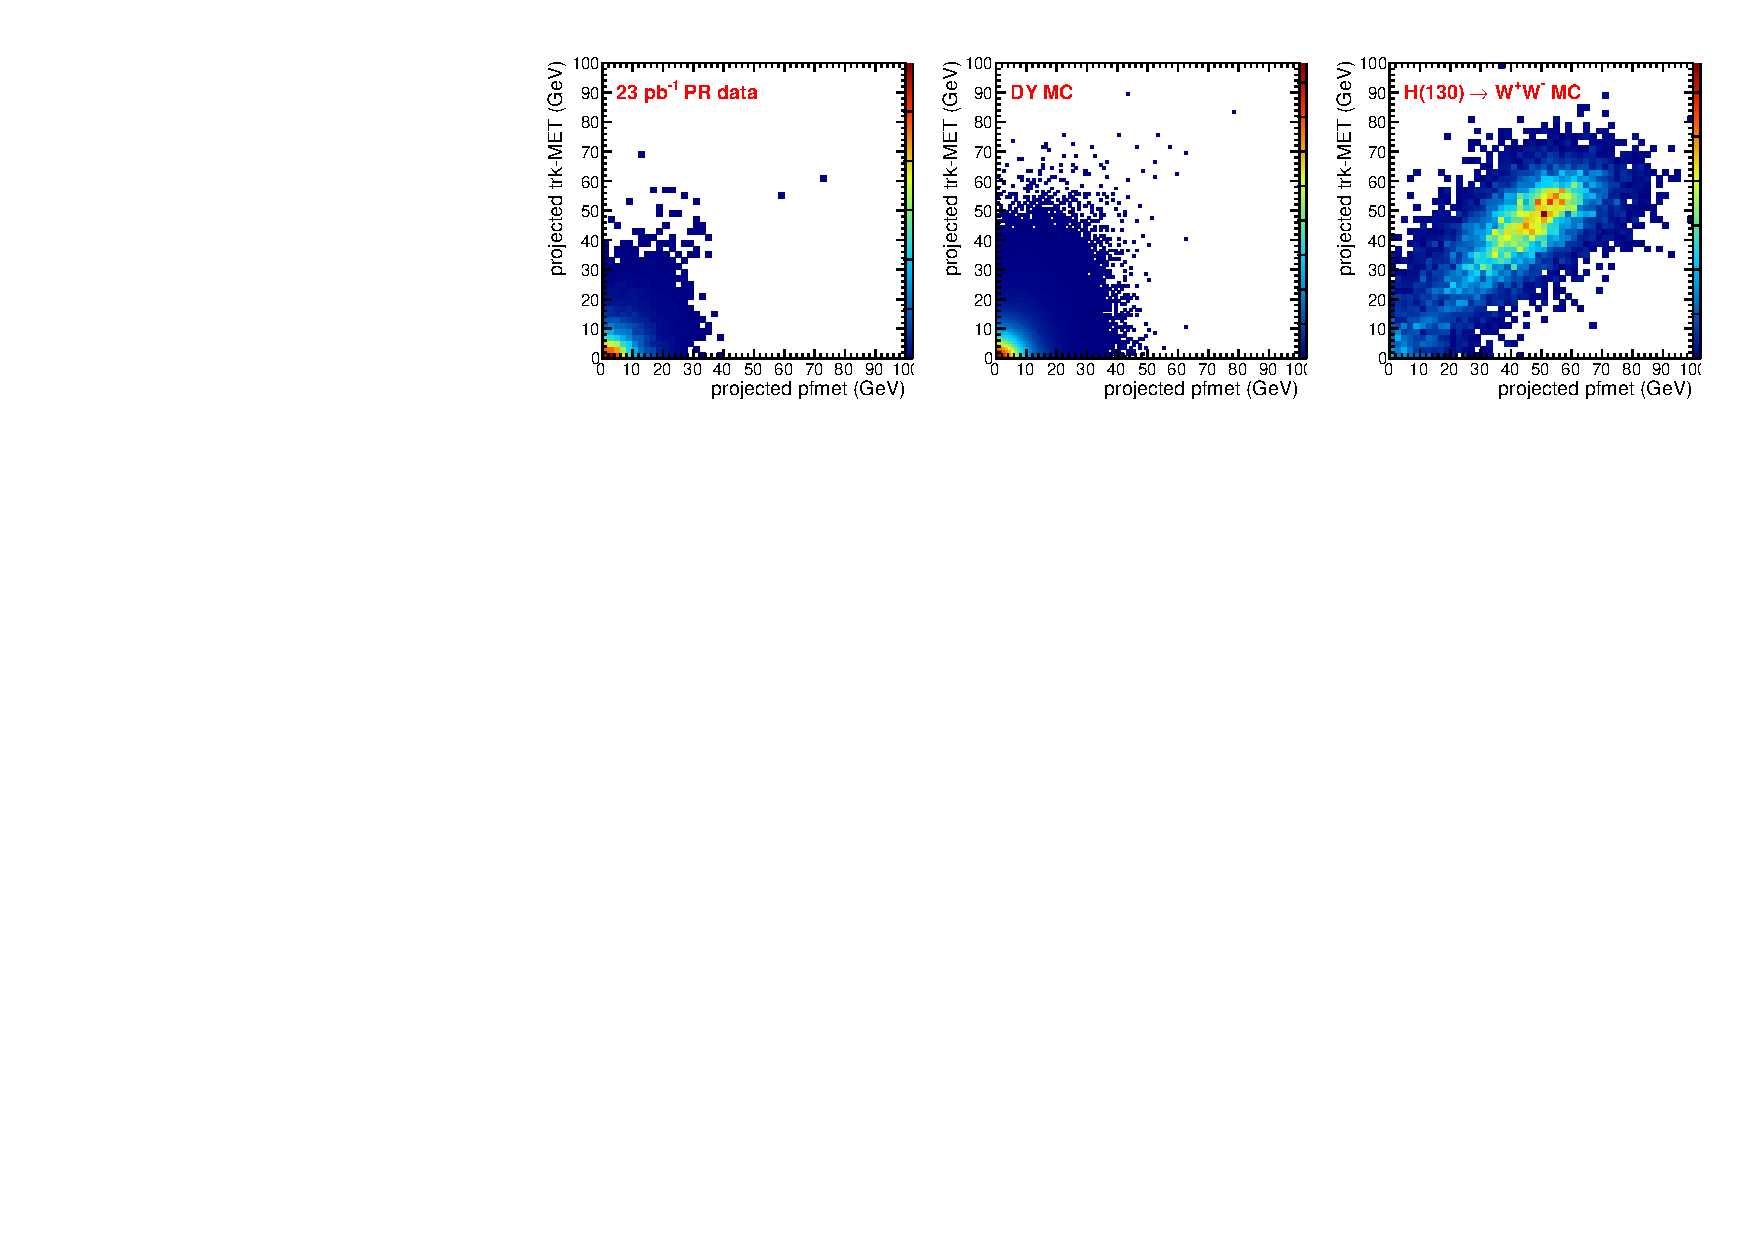
\includegraphics[width=1\linewidth]{figures/met_scatter.pdf} 
\caption{\label{fig:met_scatter}\protect Distributions of trk-MET vs. pfmet in data (left), $\dyll$ MC (center) and Higgs MC (right).}
\end{center}
\end{figure}
%%%%%%%%%%%%%%%%%%%%%%%%%%%%%%%%%%%%%%%%%%%

%%%%%%%%%%%%%%%%%%%%%%%%%%%%%%%%%%%%%%%%%%% 
\begin{figure}[hbt]
\begin{center}
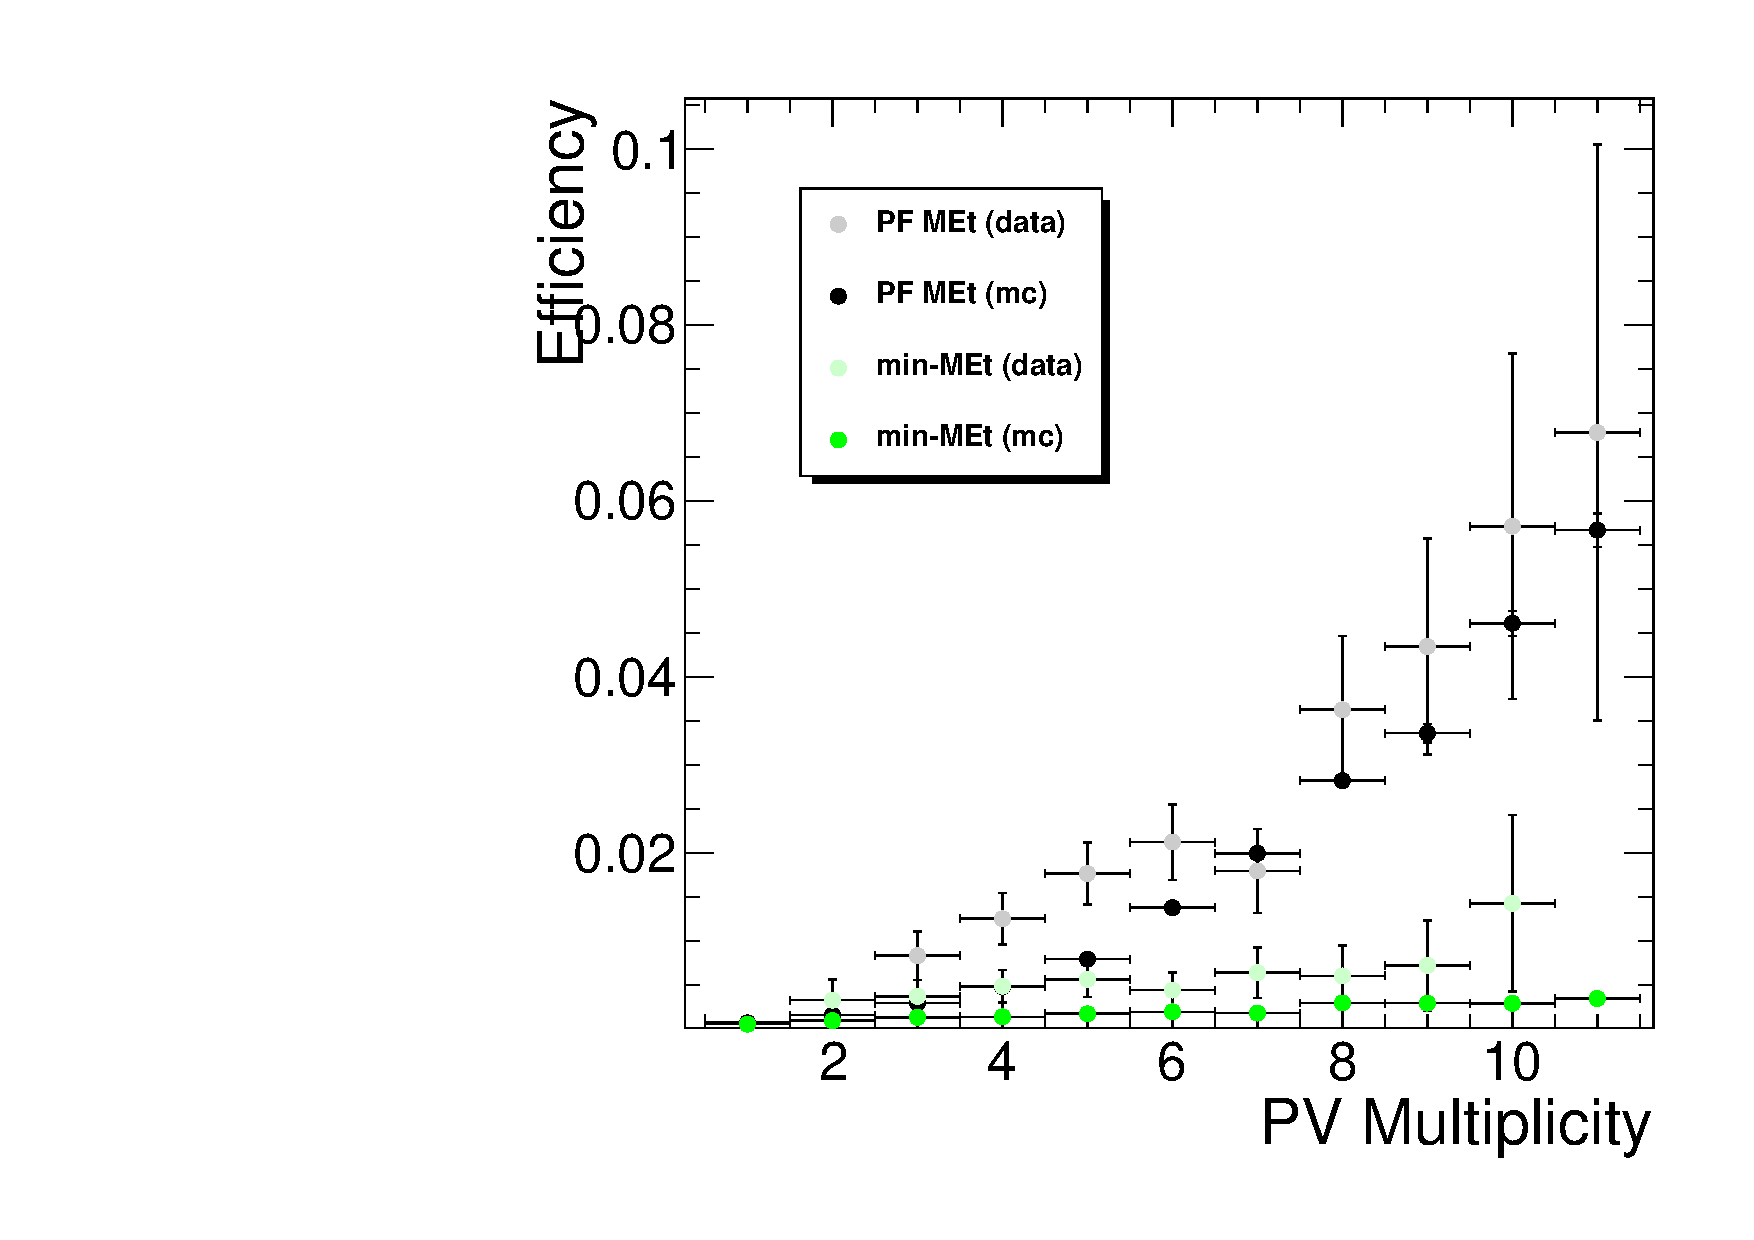
\includegraphics[width=0.45\linewidth]{figures/pfmet_minmet_Eff30.pdf} 
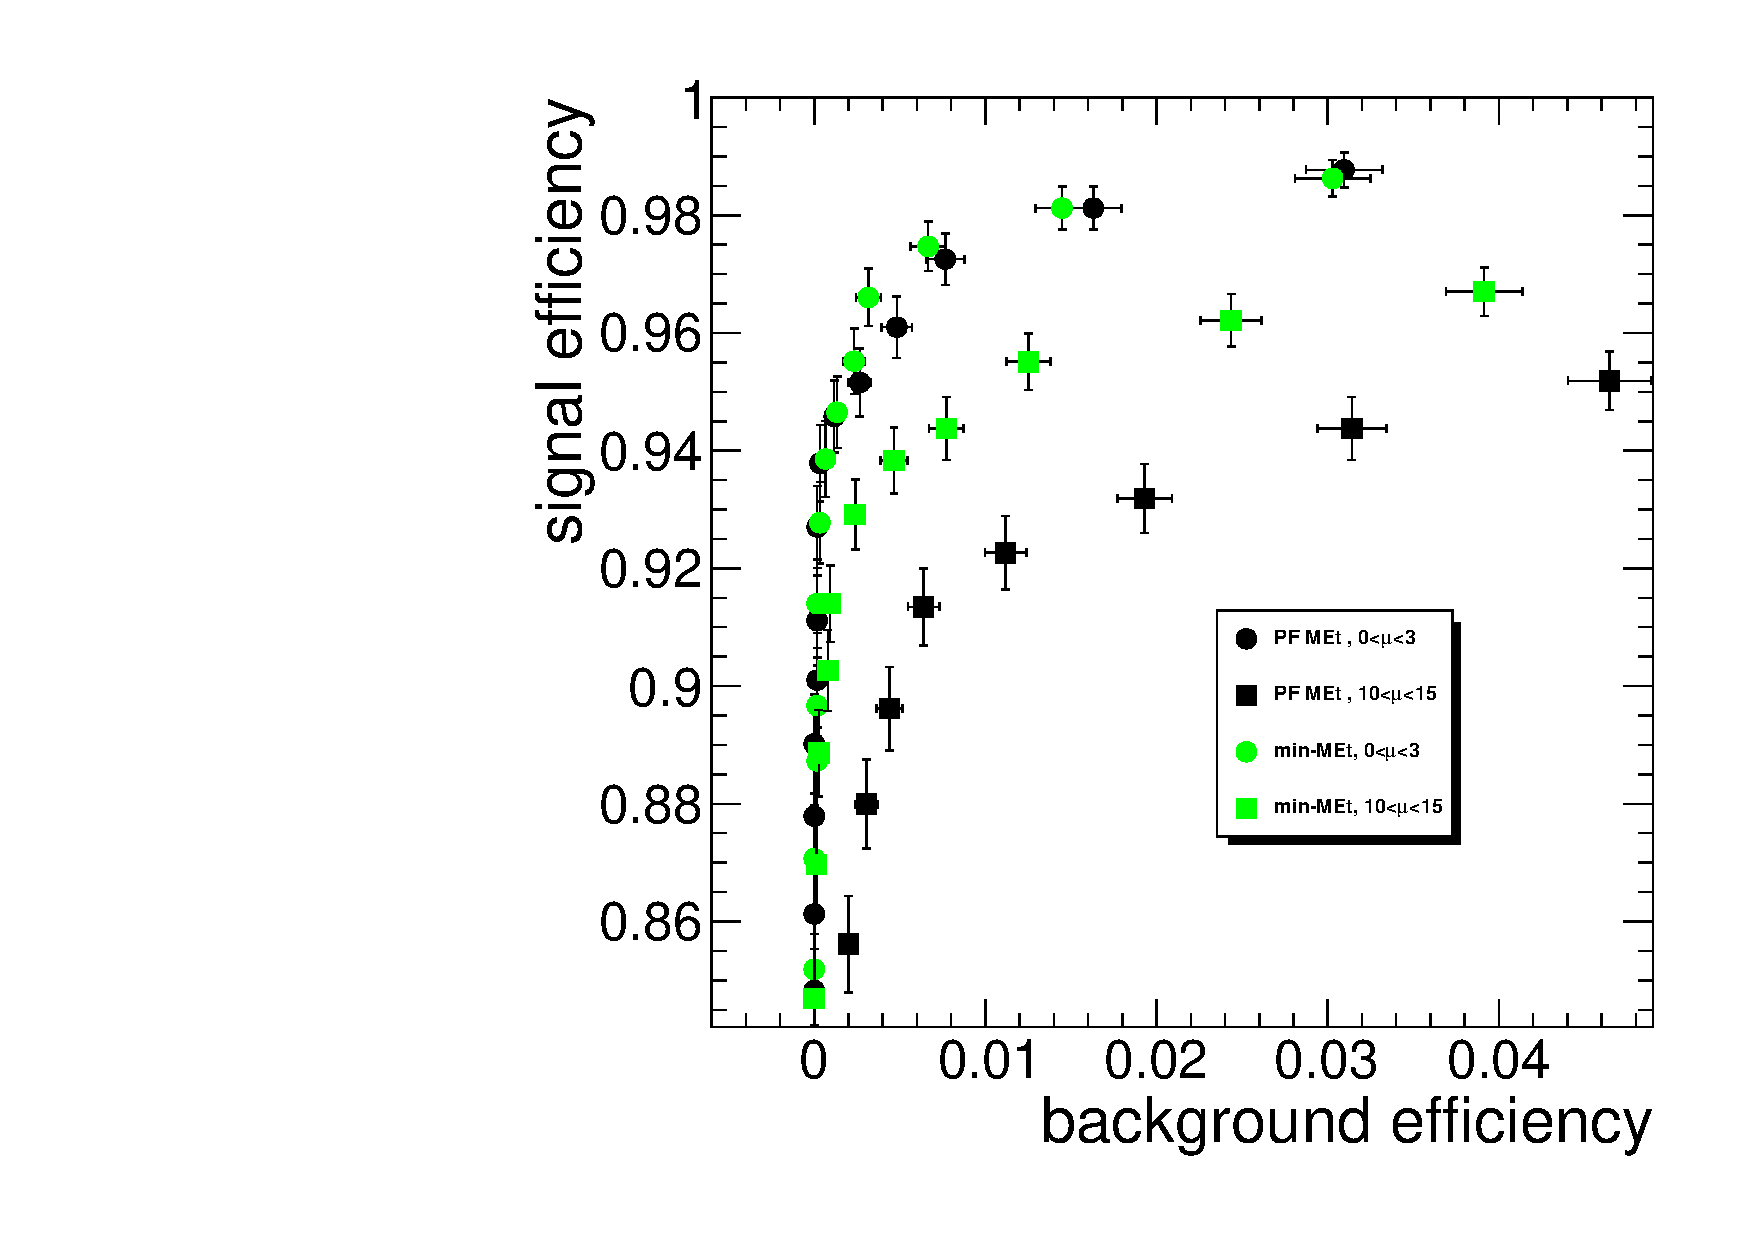
\includegraphics[width=0.45\linewidth]{figures/SignalVsBkgrEfficiency.pdf} 
\caption{\label{fig:met_eff}\protect Left plot shows the efficiency to satisfy
 the requirement pfmet$>$X~GeV as a function of the number of reconstructed 
vertices for Z-events in data and MC. Right plot shows the signal efficiency 
vs. background efficiency, evaluated for H$_{130}$ and $\dyll$ MC.}
\end{center}
\end{figure}
%%%%%%%%%%%%%%%%%%%%%%%%%%%%%%%%%%%%%%%%%%%



%In the presence of high pile-up, the instrumental \met\ tail in $\dyll$ events is enhanced
%significantly, as shown in Figure~\ref{fig:met_pu} for data and $\dyll$ MC. This causes a sharp increase in the
%efficiency for $\dyll$ events to pass a given \met\ requirement as the number of pile-up
%interactions increases. To improve the robustness of the \met\ performance
%in the presence of pile-up, we have developed a novel \met\ algorithm (trk-MET).
%trk-MET is \met\ constructed from charged particles consistent with originating from
%the signal PV. We correct for the 2 leptons, as well as charged PFCandidates which satisfy
%the following requirements:
%\begin{itemize}
%\item the track matched to PFCandidate has $\Delta z < 0.1$~cm with respect to the signal PV;
%\item the signal PV is the closest PV to the track in $\Delta z$;
%\item the track has $\Delta R > 0.1$ with respect to both leptons, to avoid 
%double-counting of the leptons.
%\end{itemize}
%The high \met\ tail in events with no genuine \met\ is larger for trk-MET than for pfmet. However,
%we observe that for data and MC $\dyll$ events these two \met\ flavors are weakly-correlated, as shown
%in Figure~\ref{fig:met_scatter}. Therefore the rejection power for $\dyll$ events is increased significantly
%by cutting on both pfmet and trk-MET, or equivalently by cutting on min-MET $\equiv$ minimum(pfmet,trk-MET).
%In addition, the high \met\ tail efficiency vs. number of pile-up interactions is flattened, as shown
%in Figure~\ref{fig:met_eff}. For signals with genuine \met\, trk-MET and pfmet are strongly correlated. 
%The signal (H(130) MC) efficiency vs. background ($\dyll$ MC) efficiency is shown in 
%Figure~\ref{fig:met_eff} for min-MET and pfmet.

  \subsection{Jet Counting} 
    \label{sec:sel_jets}
    %To split the analysis in different jet bins, we count events 
%containing jets with $\pt > ~30~\GeV$ within $|\eta|<5.0$. 

We analyze the events separately based on the number of reconstructed 
jets with $\pt > ~30~\GeV$ within $|\eta|<5.0$ in the event. 
Jets are reconstructed using calorimeter and tracker information using a particle flow 
algorithm~\cite{jetpas}. The anti-${\rm k_T}$ clustering algorithm~\cite{antikt} 
with ${\rm R=0.5}$ is used. We apply the standard jet energy 
corrections~\cite{jes} to the reconstructed jets, where the L1 Fast Jets 
corrections are included. The latter corrections are rather important since 
they help in flatening the reconstruction efficiency as a function of the 
number of overlapping events.
To exclude electrons and muons from the jet sample, these 
jets are required to be separated from the selected leptons in $\Delta R$ 
by at least $\Delta R^{\mathrm{jet-lepton}}>0.3$.

%In the 0-Jet bin, the performance of the jet veto 
%is validated on data using Drell-Yan events, 
%as will be explained in Sec.~\ref{sec:backgrounds}. 

  \subsection{Top Tagging}
    \label{sec:sel_toptag}
    
Since the top quark production cross-section is substantially higher than the
diboson production cross-section, top backgrounds generally pose a significant 
challenge for dilepton plus \met analyses. To reduce the top background, 
we use a combination of two top tagging methods implemented and commissioned in the $\hww$ 
analysis~\cite{HWW2011AN}, both relying on the fact that top quarks 
decay to $Wb$ with almost certainty.

The first method vetoes events containing soft muons from the $b$-quark decays 
The requirements used to select soft muons are:
%%%%%%%%%%%%
\begin{itemize}
    \item $\pt > 3$ GeV;
    \item Reconstructed as a TrackerMuon
    \item Meets $\mathrm{TMLastStationAngTight}$ muon id requirements
    \item The number of valid inner tracker hits $>10$
    \item The transverse impact parameter with respect to the Primary Vertex, $|d_{0}| < 0.2$~cm,
    \item The longitudinal impact parameter with respect to the Primary Vertex, $|d_{z}| < 0.2$~cm,
    \item Non-isolated $({\rm{Iso}_{Total}}/{\pt}~>~0.1)$ if $\pt>20\GeV$.
\end{itemize}
%%%%%%%%%%%%

The second method uses standard $b$-jet tagging. 
The jets are reconstructed using calorimeter and tracker information using a particle flow 
algorithm~\cite{jetpas}. The anti-${\rm k_T}$ clustering algorithm~\cite{antikt} 
with ${\rm R=0.5}$ is used. We apply the standard jet energy 
corrections~\cite{jes} to the reconstructed jets, where the L1 Fast Jets 
corrections are included. The latter corrections are rather important since 
they help in flatening the reconstruction efficiency as a function of the 
number of overlapping events.
In this method, events containing jets with $E_T>30\GeV$ tagged with
 the $\mathrm{TrkCountingHighEff}$~\cite{btag} algorithm with
a discriminator value of greater than 2.0 are vetoed. 
	

%The algorithm is applied to jets with the same definition as Section \ref{sec:sel_jets},
%with the exception that the $E_T$ requirement is removed. 
%Thus, events in the zero-jet bin can still contain tagged jets.

%As a comparison of performance , the $\WW$ signal efficiency versus the $\ttbar$ efficiency in 
%events with no jets according to the definition in Section \ref{sec:sel_jets} for different 
%standard b-tagging algorithms  is shown in Figure~\ref{fig:eff_btag_tt_ww}. 
%For a top rejection efficiency above $40\%$,
%the $\mathrm{TrkCountingHighEff}$ tagger performs better than the others.
%Our current cut value has a $\WW$ signal efficiency of about $98.1\%$ and
%a $\ttbar$ efficiency of about $39\%$.

%%%%%%%%%%%%
%\begin{figure}[!htbp]
%\begin{center}
%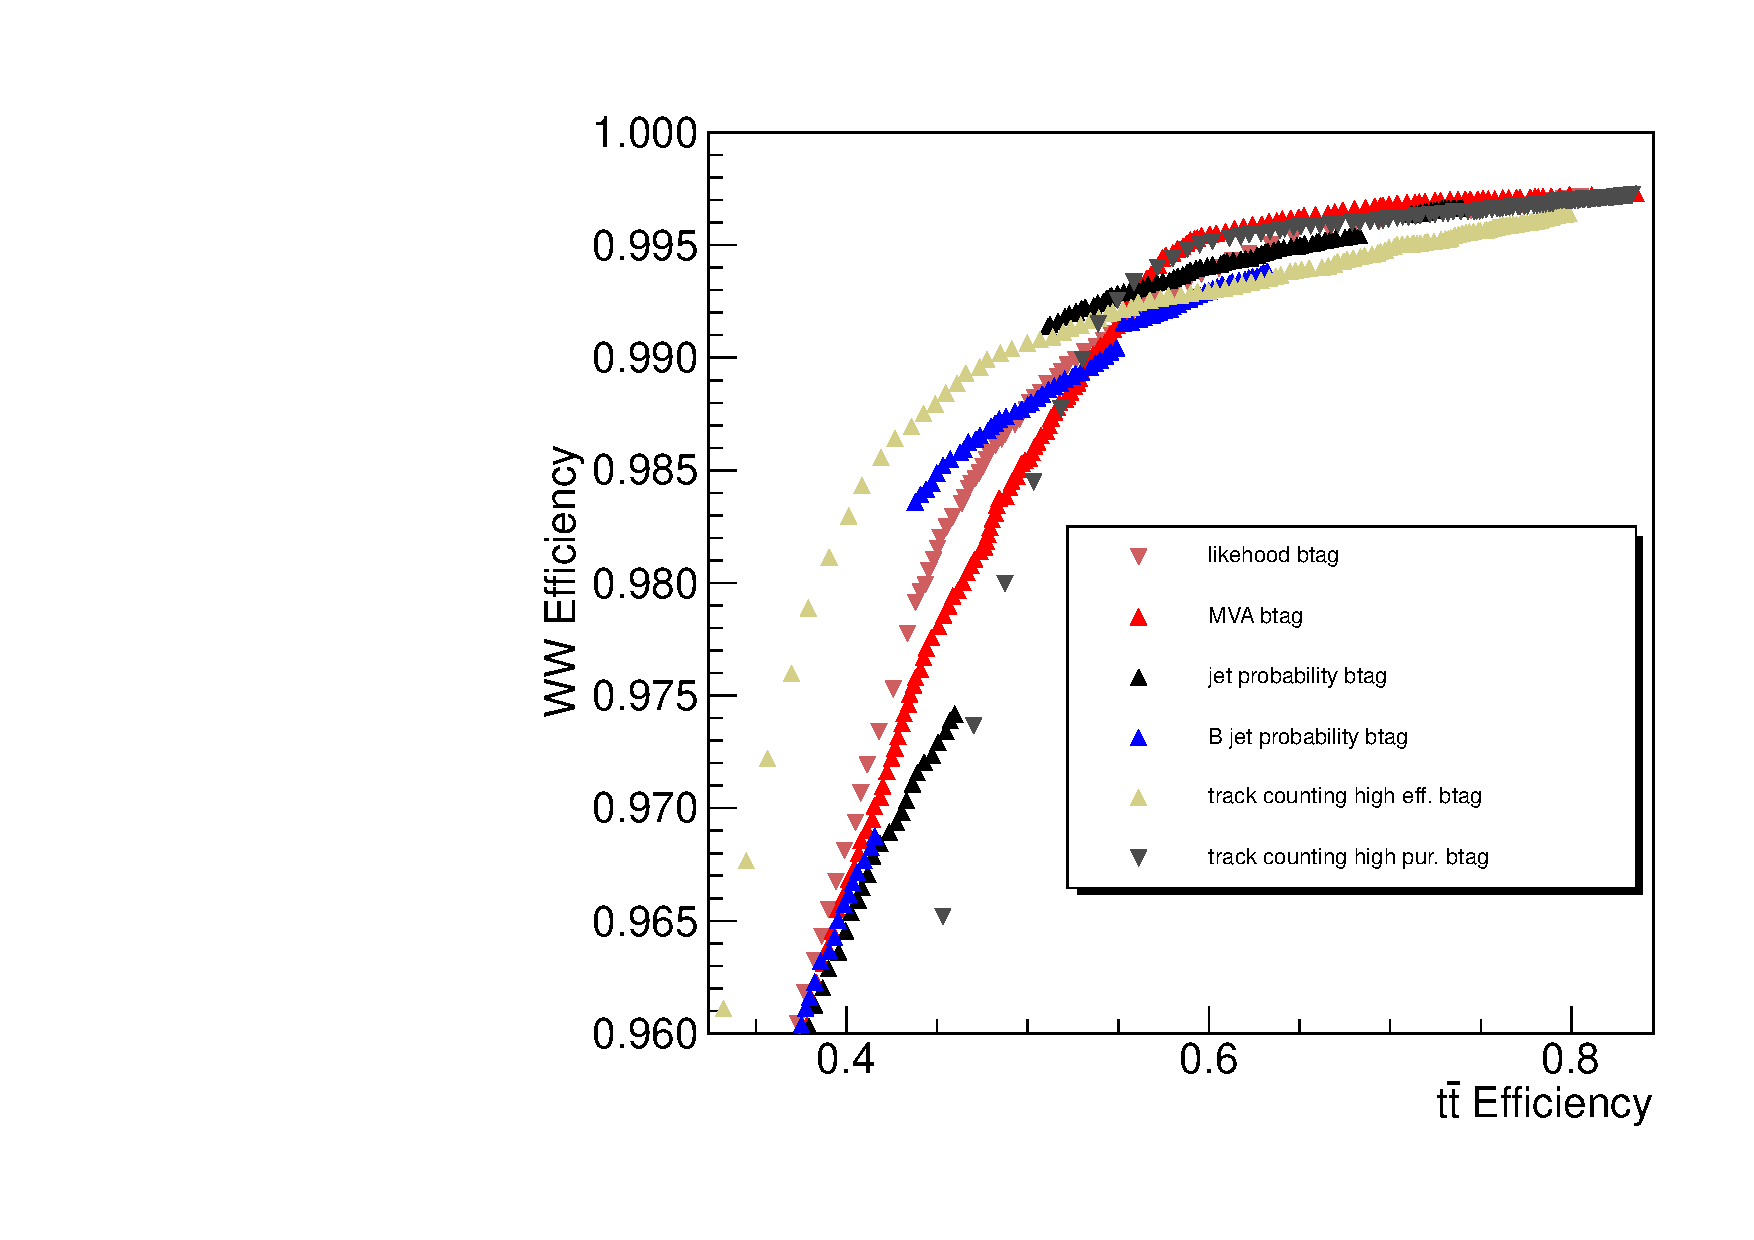
\includegraphics[width=0.60\textwidth]{figures/eff_btag_tt_ww.pdf}
%\caption{$\WW$ signal efficiency versus $\ttbar$ efficiency in events with no
%reconstructed jets for different standard b-tagging algorithms.}
%\label{fig:eff_btag_tt_ww}
%\end{center}
%\end{figure}
%%%%%%%%%%%%

%By using the expected tagging efficiency for the two methods,
%it is possible to estimate the residual top background after the vetoes
%have been applied. 
%This is described in detail in Section \ref{sec:bkg_top}.

%  \subsection{Third Lepton Veto}
  \subsection{Additional Topological Selections}
    \label{sec:sel_other}
    To reduce the background from diboson processes, we veto events
containing an additional lepton meeting the previously described
selection requirements with $\pt > 10~\GeV$.  This removes $\sim
60\%$ of the $WZ$ component and $\sim 10\%$ of the $ZZ$ one.  The \ZZ\
component is dominated by $\ZZ \to 2l2\nu$ decays. The efficiency for
$WW \to 2l2\nu$ events is $\sim 99.9\%$.  Finally, in the events 
containing 2 or more jets, the angle in the transverse plane between 
the dilepton system and the system of two most energetic jets with 
$\pt^{jet}~>~15~\GeV$ must be smaller than $165$ degrees in
the $ee/\mu\mu$ final states. This requirement rejects $\dyll$
events, where the $\Z$ boson recoil against jets.
In the events with 0 or 1 jets, this variable is used as an input 
to the MVA-based Drell-Yan suppression technique.



\clearpage

\section{Expected Event Yields After $\zz$ Preselection}
  \label{sec:yields_mc}
  
The expected number of signal and background events for an integrated 
luminosity of 1\ifb{} after applying the $\ZZ$ like selection are reported in 
Tables~\ref{tab:mcyield_zzsel_0j}(0-jet),~\ref{tab:mcyield_zzsel_1j}(1-jet), 
~\ref{tab:mcyield_zzsel_2j}(2-jet), 
%The angle between the dilepton system and the jet in the transverse plane must be 
%smaller than 165 degrees. The \hzz simulated events are reweighted to match the 
%Higgs $\pt$ at NNLO, as explained in Section~\ref{sec:datasets}; 
%all data-driven corrections are not applied. 
%The corresponding $\Delta\phi$, di-lepton mass, di-lepton $p_T$, $m_T$ and projected 
%$\met$ distributions are shown in Figs.~\ref{fig:dPhi_jets0}-\ref{fig:pmet_jets0}(0-jet) 
%and Figs.~\ref{fig:dPhi_jets1}-\ref{fig:pmet_jets1}(1-jet).


%%%%%%%%%%%%%
\begin{table}[!ht]
\begin{center}
\begin{tabular}{c|c|c|c}
\hline
sample    & $\mu\mu$    & ee     & TOTAL\\ \hline 
hzz300   & 2.37 $\pm$ 0.03   & 1.74 $\pm$ 0.02   & 4.11 $\pm$ 0.03 \\ \hline 
hww300   & 0.70 $\pm$ 0.02   & 0.54 $\pm$ 0.02   & 1.24 $\pm$ 0.03 \\ \hline 
wjets   & 0.00 $\pm$ 0.00   & 0.99 $\pm$ 0.44   & 0.99 $\pm$ 0.44 \\ \hline 
qqww   & 8.05 $\pm$ 0.22   & 5.63 $\pm$ 0.19   & 13.68 $\pm$ 0.29 \\ \hline 
ggww   & 0.50 $\pm$ 0.03   & 0.37 $\pm$ 0.02   & 0.87 $\pm$ 0.03 \\ \hline 
wz   & 6.72 $\pm$ 0.24   & 4.06 $\pm$ 0.19   & 10.78 $\pm$ 0.31 \\ \hline 
zz   & 13.11 $\pm$ 0.22   & 9.08 $\pm$ 0.18   & 22.20 $\pm$ 0.28 \\ \hline 
ttbar   & 0.96 $\pm$ 0.36   & 0.41 $\pm$ 0.24   & 1.37 $\pm$ 0.43 \\ \hline 
tw   & 0.48 $\pm$ 0.10   & 0.39 $\pm$ 0.09   & 0.88 $\pm$ 0.14 \\ \hline 
zeejets   & 0.00 $\pm$ 0.00   & 0.00 $\pm$ 0.00   & 0.00 $\pm$ 0.00 \\ \hline 
zmmjets   & 0.84 $\pm$ 0.84   & 0.00 $\pm$ 0.00   & 0.84 $\pm$ 0.84 \\ \hline 
zttjets   & 0.00 $\pm$ 0.00   & 0.00 $\pm$ 0.00   & 0.00 $\pm$ 0.00 \\ \hline 
%gamma   & 0.00 $\pm$ 0.00   & 0.00 $\pm$ 0.00   & 0.00 $\pm$ 0.00 \\ \hline 
SIGNAL   & 2.37 $\pm$ 0.03   & 1.74 $\pm$ 0.02   & 4.11 $\pm$ 0.03 \\ \hline 
BKGD   & 31.37 $\pm$ 1.00   & 21.48 $\pm$ 0.60   & 52.85 $\pm$ 1.17 \\ \hline 
\end{tabular}
\caption{Expected number of signal and background events for an 
  integrated luminosity of 1\ifb{} after applying the \zz\ 
  0-jet selection requirements. Monte Carlo statistical 
  uncertainties are included.}
\label{tab:mcyield_zzsel_0j}
\end{center}
\end{table}
%%%%%%%%%%%%%


%%%%%%%%%%%%%
\begin{table}[!ht]
\begin{center}
\begin{tabular}{c|c|c|c}
\hline
sample    & $\mu\mu$    & ee     & TOTAL\\ \hline 
hzz300   & 1.35 $\pm$ 0.02   & 0.97 $\pm$ 0.02   & 2.32 $\pm$ 0.02 \\ \hline 
hww300   & 0.45 $\pm$ 0.02   & 0.31 $\pm$ 0.01   & 0.76 $\pm$ 0.02 \\ \hline 
wjets   & 0.00 $\pm$ 0.00   & 0.00 $\pm$ 0.00   & 0.00 $\pm$ 0.00 \\ \hline 
qqww   & 2.55 $\pm$ 0.13   & 1.88 $\pm$ 0.11   & 4.43 $\pm$ 0.17 \\ \hline 
ggww   & 0.17 $\pm$ 0.02   & 0.12 $\pm$ 0.01   & 0.30 $\pm$ 0.02 \\ \hline 
wz   & 3.28 $\pm$ 0.17   & 2.45 $\pm$ 0.15   & 5.73 $\pm$ 0.22 \\ \hline 
zz   & 3.33 $\pm$ 0.11   & 2.44 $\pm$ 0.09   & 5.77 $\pm$ 0.14 \\ \hline 
ttbar   & 2.20 $\pm$ 0.55   & 1.92 $\pm$ 0.51   & 4.12 $\pm$ 0.75 \\ \hline 
tw   & 0.66 $\pm$ 0.12   & 0.68 $\pm$ 0.12   & 1.34 $\pm$ 0.17 \\ \hline 
zeejets   & 0.00 $\pm$ 0.00   & 0.86 $\pm$ 0.86   & 0.86 $\pm$ 0.86 \\ \hline 
zmmjets   & 1.68 $\pm$ 1.19   & 0.00 $\pm$ 0.00   & 1.68 $\pm$ 1.19 \\ \hline 
zttjets   & 0.00 $\pm$ 0.00   & 0.00 $\pm$ 0.00   & 0.00 $\pm$ 0.00 \\ \hline 
%gamma   & 0.00 $\pm$ 0.00   & 0.00 $\pm$ 0.00   & 0.00 $\pm$ 0.00 \\ \hline 
SIGNAL   & 1.35 $\pm$ 0.02   & 0.97 $\pm$ 0.02   & 2.32 $\pm$ 0.02 \\ \hline 
BKGD   & 14.31 $\pm$ 1.34   & 10.68 $\pm$ 1.03   & 24.99 $\pm$ 1.69 \\ \hline 
\end{tabular}
\caption{Expected number of signal and background events for an 
  integrated luminosity of 1\ifb{} after applying the \zz\ 
  1-jet selection requirements. Monte Carlo statistical 
  uncertainties are included.}
\label{tab:mcyield_zzsel_1j}
\end{center}
\end{table}
%%%%%%%%%%%%%

%%%%%%%%%%%%%
\begin{table}[!ht]
\begin{center}
\begin{tabular}{c|c|c|c}
\hline
sample    & $\mu\mu$    & ee     & TOTAL\\ \hline 
hzz300   & 0.44 $\pm$ 0.01   & 0.33 $\pm$ 0.01   & 0.77 $\pm$ 0.01 \\ \hline 
hww300   & 0.20 $\pm$ 0.01   & 0.15 $\pm$ 0.01   & 0.35 $\pm$ 0.01 \\ \hline 
wjets   & 0.00 $\pm$ 0.00   & 0.00 $\pm$ 0.00   & 0.00 $\pm$ 0.00 \\ \hline 
qqww   & 0.80 $\pm$ 0.07   & 0.49 $\pm$ 0.06   & 1.29 $\pm$ 0.09 \\ \hline 
ggww   & 0.03 $\pm$ 0.01   & 0.03 $\pm$ 0.01   & 0.05 $\pm$ 0.01 \\ \hline 
wz   & 1.42 $\pm$ 0.11   & 1.04 $\pm$ 0.09   & 2.46 $\pm$ 0.15 \\ \hline 
zz   & 0.90 $\pm$ 0.06   & 0.60 $\pm$ 0.05   & 1.50 $\pm$ 0.07 \\ \hline 
ttbar   & 3.57 $\pm$ 0.70   & 0.96 $\pm$ 0.36   & 4.54 $\pm$ 0.79 \\ \hline 
tw   & 0.31 $\pm$ 0.08   & 0.18 $\pm$ 0.06   & 0.48 $\pm$ 0.10 \\ \hline 
zeejets   & 0.00 $\pm$ 0.00   & 4.32 $\pm$ 1.93   & 4.32 $\pm$ 1.93 \\ \hline 
zmmjets   & 7.56 $\pm$ 2.52   & 0.00 $\pm$ 0.00   & 7.56 $\pm$ 2.52 \\ \hline 
zttjets   & 0.00 $\pm$ 0.00   & 0.00 $\pm$ 0.00   & 0.00 $\pm$ 0.00 \\ \hline 
%gamma   & 0.00 $\pm$ 0.00   & 0.00 $\pm$ 0.00   & 0.00 $\pm$ 0.00 \\ \hline 
SIGNAL   & 0.44 $\pm$ 0.01   & 0.33 $\pm$ 0.01   & 0.77 $\pm$ 0.01 \\ \hline 
BKGD   & 14.78 $\pm$ 2.62   & 7.76 $\pm$ 1.97   & 22.54 $\pm$ 3.28 \\ \hline 
\end{tabular}
\caption{\fixme{}Expected number of signal and background events for an 
  integrated luminosity of 1\ifb{} after applying the \zz\ 
  2-jet selection requirements. Monte Carlo statistical 
  uncertainties are included.}
\label{tab:mcyield_zzsel_2j}
\end{center}
\end{table}
%%%%%%%%%%%%%

\clearpage    

\section{Higgs Signal Extraction Strategy}
  To enhance the sensitivity to the Higgs boson signal, two different approaches 
are performed. The first one is a cut-based approach where further requirements 
on a few observables are applied, while the second one makes use of
multivariate techniques. Both of them cover a large Higgs boson mass
($m_{\rm{H}}$) range, and each is separately optimized for different
$m_{\rm{H}}$ hypotheses. The first method is the simplest approach with smaller
systematic uncertainties. The second one is
more powerful, since it exploits the information present in the
correlation among the variables. 



%% The quoted results in this section are scaled to 1 $\ifb$ of integrated luminosity. 
%% The background yields have been scaled taking into account the observed data 
%% corrections, discussed in Section~\ref{sec:backgrounds}, with the current data 
%% sample to give realistic estimations, while $gg \to H \to ZZ$ simulated 
%% events are reweighted to match the Higgs $\pt$ at NNLO, as explained in 
%% Section~\ref{sec:datasets}. 

%% Stuff to add in the MVA later
%To enhance the sensitivity to the Higgs boson signal, two different approaches 
%are performed. The first one is a cut-based approach where further requirements 
%on a few observables are applied, while the second one makes use of
%multivariate techniques. Both of them cover a large Higgs boson mass
%($m_{\rm{H}}$) range, and each is separately optimized for different
%$m_{\rm{H}}$ hypotheses. The first method is the simplest approach with smaller
%systematic uncertainties. The second one is
%more powerful, since it exploits the information present in the
%correlation among the variables. 

%Output of the multivariate discriminator has two different use
%cases. In the first case we use it as just one more variable to cut on
%in the cut-based analysis. In the second case we use the discriminator
%output distribution for the final signal extraction.

%All analyses are further split in the corresponding 0-jet, 1-jet and
%2-jet bins. In the 2-jet bin we use a simple cut-based approach for
%now due to the limited sensitivity and the limited number of events in
%simulation.


  \label{sec:signal_selection}
  \subsection{Cut Based Analysis}
    \label{sec:anal_cutbased}
    
To enhance the sensitivity to the Higgs boson signal, we apply additional 
$m_{\rm{H}}$ hypothesis dependent selections on the 
minimum $\met$ and Higgs transverse mass ($M_{T}$) observables, 
covering a large Higgs boson mass ($m_{\rm{H}}$) range. 

The transverse mass is defined by

\begin{equation}
M_{T}^{2} = (\sqrt{p_{T\mathrm{ ll}}^{2} + M_{ll}^{2}} + \sqrt{(\met)^{2} + M_{ll}^{2}})^{2} - (\vec{p_{T\mathrm{ ll}}} + \vec{\met})^{2}. \\
\label{eq:MTHZZ}
\end{equation}

The higgs selection cuts are optimized for the significance ($S/\sqrt{S+B}$)
separately in the 0-jet and 1-jet. The values of the cuts are summarized in
Tables \ref{tab:HiggsSelectionCutBased_0j} and \ref{tab:HiggsSelectionCutBased_1j} for the 0-jet and 1-jet bins. 
A one sided cut is applied on the minimum \met and a two sided cut is applied on the transverse mass. 

%%%%%%%%%%%%%
\begin{table}[!ht]
\begin{center}
\begin{tabular}{c|c|c|c}
\hline
Higgs Mass        & Min $\met$ Cut Value  & Min $\mt$ Cut Value   & Max $\mt$ Cut Value \\ 
\hline 
%200               & $> 50$ GeV            & $> 180$ GeV            & $< 220$ GeV          \\ \hline 
250               & $> 60$ GeV            & $> 220$ GeV            & $< 260$ GeV          \\ \hline 
300               & $> 70$ GeV            & $> 260$ GeV            & $< 320$ GeV          \\ \hline 
400               & $> 70$ GeV            & $> 260$ GeV            & $< 320$ GeV          \\ \hline 
\end{tabular}
\caption{Expected number of signal and background events for an 
  integrated luminosity of 1\ifb{} after applying the \zz\ 
  0-jet selection requirements. Monte Carlo statistical 
  uncertainties are included.}
\label{tab:HiggsSelectionCutBased_0j}
\end{center}
\end{table}
%%%%%%%%%%%%%

%%%%%%%%%%%%%
\begin{table}[!ht]
\begin{center}
\begin{tabular}{c|c|c|c}
\hline
Higgs Mass        & Min $\met$ Cut Value  & Min $\mt$ Cut Value   & Max $\mt$ Cut Value \\ 
\hline 
%200               & $> 60$ GeV            & $> 180$ GeV            & $< 200$ GeV          \\ \hline 
250               & $> 60$ GeV            & $> 180$ GeV            & $< 260$ GeV          \\ \hline 
300               & $> 100$ GeV           & $> 260$ GeV            & $< 320$ GeV          \\ \hline 
400               & $> 100$ GeV           & $> 300$ GeV            & $< 450$ GeV          \\ \hline 
\end{tabular}
\caption{Expected number of signal and background events for an 
  integrated luminosity of 1\ifb{} after applying the \zz\ 
  1-jet selection requirements. Monte Carlo statistical 
  uncertainties are included.}
\label{tab:HiggsSelectionCutBased_1j}
\end{center}
\end{table}
%%%%%%%%%%%%%

%%%%%%%%%%%%%
%\begin{table}[!ht]
%\begin{center}
%\begin{tabular}{c|c|c|c}
%\hline
%Higgs Mass        & Min $\met$ Cut Value  & Min $\mt$ Cut Value   & Max $\mt$ Cut Value \\ 
%\hline 
%%200               & $> 80$ GeV            & $> 180$ GeV            & $< 200$ GeV          \\ \hline 
%250               & $> 80$ GeV            & $> 180$ GeV            & $< 260$ GeV          \\ \hline 
%300               & $> 100$ GeV           & $> 240$ GeV            & $< 320$ GeV          \\ \hline 
%400               & $> 100$ GeV           & $> 300$ GeV            & $< 450$ GeV          \\ \hline 
%\end{tabular}
%\caption{Expected number of signal and background events for an 
%  integrated luminosity of 1\ifb{} after applying the \zz\ 
%  2-jet selection requirements. Monte Carlo statistical 
%  uncertainties are included.}
%\label{tab:HiggsSelectionCutBased_2j}
%\end{center}
%\end{table}
%%%%%%%%%%%%%

Due to the missing VBF production samples for the signal in our Spring11 set of 
Monte Carlo samples,  we did not include the yields for the VBF contribution. 
In Table \ref{tab:VBFSignalContribution} we summarize the expected VBF contribution to the signal yield
estimated from the Summer11 Monte Carlo samples.
We do not perform any scaling based on these expectations.
Because we could not make a meaningful choice of cuts for the 2-jet bin,
we temporarily dropped it from this analysis.

%%%%%%%%%%%%%
\begin{table}[!ht]
\begin{center}
\begin{tabular}{|c|c|c|}
\hline
Higgs Mass        & Relative VBF Contribution in 0-Jet Bin & Relative VBF Contribution in 1-Jet Bin \\ 
\hline 
250               & $1.8\%$                                & $11\%$                                 \\ 
300               & $1.9\%$                                & $9.8\%$                                \\ 
\hline 
\end{tabular}
\caption{Expected relative contribution from the VBF production process to the total
expected signal yield.}
\label{tab:VBFSignalContribution}
\end{center}
\end{table}
%%%%%%%%%%%%%


%% The quoted results in this section are scaled to 1 $\ifb$ of integrated luminosity. 
%% The background yields have been scaled taking into account the observed data 
%% corrections, discussed in Section~\ref{sec:backgrounds}, with the current data 
%% sample to give realistic estimations, while $gg \to H \to ZZ$ simulated 
%% events are reweighted to match the Higgs $\pt$ at NNLO, as explained in 
%% Section~\ref{sec:datasets}. 

%% Stuff to add in the MVA later
%To enhance the sensitivity to the Higgs boson signal, two different approaches 
%are performed. The first one is a cut-based approach where further requirements 
%on a few observables are applied, while the second one makes use of
%multivariate techniques. Both of them cover a large Higgs boson mass
%($m_{\rm{H}}$) range, and each is separately optimized for different
%$m_{\rm{H}}$ hypotheses. The first method is the simplest approach with smaller
%systematic uncertainties. The second one is
%more powerful, since it exploits the information present in the
%correlation among the variables. 

%Output of the multivariate discriminator has two different use
%cases. In the first case we use it as just one more variable to cut on
%in the cut-based analysis. In the second case we use the discriminator
%output distribution for the final signal extraction.

%All analyses are further split in the corresponding 0-jet, 1-jet and
%2-jet bins. In the 2-jet bin we use a simple cut-based approach for
%now due to the limited sensitivity and the limited number of events in
%simulation.


%    \subsubsection{0-Jet Selection}
%      \label{sec:sel_zerojet}
     % After the $\WW$ selection, the following handles are used to discriminate
against the remaining background, specially $\WW$ continuum:

\begin{itemize}
\item the angle $\delphill$ between the two selected leptons in the transverse 
plane. This variable provides the best discriminating 
power between the Higgs signal and the majority of the backgrounds for 
$\hww$ production in the low Higgs boson mass range. Leptons originating from 
$\hww$ decays tend to have a relatively small opening angle, while those from 
backgrounds are preferentially emitted back-to-back. The importance of this 
variable decreases for high masses, since the boost of the $\W$ bosons 
dilutes the angular correlation;

\item an upper cut on the invariant mass of the lepton-pair;

\item a lower cut on the transverse momenta of the harder (\ptlmax) and 
the softer (\ptlmin) lepton;

\item the transverse Higgs mass, $m_{T}^{\ell\ell\met} = \sqrt{2\pt^{ll}\met(1-cos(\ell\ell-\met))}$.

\end{itemize} 

As a reference we use 2010 analysis cut based approach documented
in~\cite{HWW2010}. Table~\ref{tab:cutanalysis0j} summarizes selection
requirements re-tuned for this analysis.

\begin{table}[!ht]
  \begin{center}
 {\small
  \begin{tabular} {|c|c|c|c|c|c|c|}
  \hline
\mHi [GeV] & $\ptlmax$ [$\GeV$] & $\ptlmin$ [$\GeV$] & $\mll$ [$\GeV$] & $\delphill$ [dg.] & $m_{T}^{\ell\ell\met}$ [GeV  \\  \hline
           &   $>$               &   $>$               &   $<$             &  $<$          &    [,]                       \\  \hline

  \hline
  \hline
  H$_{120}$ & 20 & 10 & 2.0 & 40 & [70,120]\\
  H$_{130}$ & 25 & 10 & 1.5 & 45 & [75,125]\\
  H$_{140}$ & 25 & 15 & 1.5 & 45 & [80,130]\\
  H$_{150}$ & 27 & 25 & 1.5 & 50 & [80,150]\\
  H$_{160}$ & 30 & 25 & 1.0 & 50 & [90,160]\\
  \hline
 \hline
  \end{tabular}
  }
  \caption{Final Event selection requirements for a cut-based analysis}
   \label{tab:cutanalysis0j}
  \end{center}
\end{table}


\begin{table}[!ht]
  \begin{center}
 {\small
  \begin{tabular} {|c|c|c|c|}
  \hline
  Mass   &  R(2020) & R(2010) & R(new) \\
  \hline
  \hline
  H$_{120}$ & 7.6 & 5.0 & 3.4 \\
  H$_{130}$ & 2.7 & 2.3 & 1.7 \\
  H$_{140}$ & 1.4 & 1.4 & 1.2 \\
  H$_{150}$ & 0.88 & 0.93 & 0.80 \\
  H$_{160}$ & 0.44 & 0.60 & 0.43 \\
  \hline


 \hline
  \end{tabular}
  }
  \caption{Cut based analysis performance for different tunes. R(2020) refers 
  to 2010 analysis with minimum lepton \pt\ of 20 GeV. R(2010) is the same set of cuts,
  but the trailing lepton \pt\ is lowered to 10 GeV for Higgs mass hypothesis 
  of 160 GeV and lower. R(new) is a new set of cuts used in this analysis.}
   \label{tab:cutanalysis_perf}
  \end{center}
\end{table}


\begin{table}[!ht]
  \begin{center}
 {\footnotesize
  \begin{tabular} {|c|c|c|c|c|c|c|c|c||c||c|}
\hline
  & DY & ttbar & TW & Wjets & WZ & ZZ & ggWW & qqWW & {\bf All bkg} & {\bf H$_{120}$}\\
  \hline
  \hline
  mm &  0.8$\pm$0.8 &  0.4$\pm$0.3 &  0.3$\pm$0.1 &  4.4$\pm$3.1 &  0.3$\pm$0.1 &  0.5$\pm$0.0 &  0.6$\pm$0.0 & 12.9$\pm$0.3 & 20.2$\pm$3.2 & 2.5$\pm$0.1 \\
  me &  0.0$\pm$0.0 &  0.7$\pm$0.3 &  0.3$\pm$0.1 &  4.4$\pm$3.1 &  0.3$\pm$0.0 &  0.0$\pm$0.0 &  0.4$\pm$0.0 &  8.4$\pm$0.2 & 14.4$\pm$3.1 & 1.5$\pm$0.0 \\
  em &  0.0$\pm$0.0 &  0.6$\pm$0.3 &  0.4$\pm$0.1 &  6.4$\pm$3.7 &  0.4$\pm$0.1 &  0.0$\pm$0.0 &  0.5$\pm$0.0 & 11.7$\pm$0.3 & 20.1$\pm$3.7 & 2.5$\pm$0.1 \\
  ee &  0.0$\pm$0.0 &  0.1$\pm$0.1 &  0.1$\pm$0.1 &  6.2$\pm$3.6 &  0.2$\pm$0.0 &  0.2$\pm$0.0 &  0.3$\pm$0.0 &  6.1$\pm$0.2 & 13.2$\pm$3.6 & 1.1$\pm$0.0 \\
 \hline
 all &  0.8$\pm$0.8 &  1.9$\pm$0.5 &  1.1$\pm$0.2 & 21.3$\pm$6.7 &  1.2$\pm$0.1 &  0.8$\pm$0.0 &  1.8$\pm$0.1 & 39.0$\pm$0.5 & 67.9$\pm$6.8 & 7.6$\pm$0.1 \\
 \hline
  \end{tabular}
  }
 {\footnotesize
  \begin{tabular} {|c|c|c|c|c|c|c|c|c||c||c|}
\hline
  & DY & ttbar & TW & Wjets & WZ & ZZ & ggWW & qqWW & {\bf All bkg} & {\bf H$_{130}$}\\
  \hline
  \hline
  mm & 0.8$\pm$0.8 &  0.3$\pm$0.2 &  0.3$\pm$0.1 &  4.4$\pm$3.1 &  0.4$\pm$0.1 &  0.5$\pm$0.0 &  0.7$\pm$0.0 & 14.5$\pm$0.3 & 21.8$\pm$3.2 & 4.9$\pm$0.1 \\
  me & 0.0$\pm$0.0 &  1.0$\pm$0.4 &  0.3$\pm$0.1 &  2.2$\pm$2.2 &  0.3$\pm$0.0 &  0.0$\pm$0.0 &  0.5$\pm$0.0 &  9.2$\pm$0.2 & 13.4$\pm$2.2 & 3.2$\pm$0.1 \\
  em & 0.0$\pm$0.0 &  0.4$\pm$0.3 &  0.5$\pm$0.1 &  2.1$\pm$2.1 &  0.4$\pm$0.1 &  0.0$\pm$0.0 &  0.6$\pm$0.0 & 12.3$\pm$0.3 & 16.3$\pm$2.1 & 4.4$\pm$0.1 \\
  ee & 0.8$\pm$0.8 &  0.1$\pm$0.1 &  0.1$\pm$0.0 &  8.2$\pm$4.1 &  0.2$\pm$0.0 &  0.2$\pm$0.0 &  0.4$\pm$0.0 &  7.1$\pm$0.2 & 17.2$\pm$4.2 & 2.4$\pm$0.1 \\
 \hline
 all & 1.6$\pm$1.1 &  1.9$\pm$0.5 &  1.2$\pm$0.2 & 16.8$\pm$5.9 &  1.2$\pm$0.1 &  0.7$\pm$0.0 &  2.2$\pm$0.1 & 43.1$\pm$0.5 & 68.9$\pm$6.1 & 15.0$\pm$0.2 \\
 \hline
  \end{tabular}
  }
 {\footnotesize
  \begin{tabular} {|c|c|c|c|c|c|c|c|c||c||c|}
\hline
  & DY & ttbar & TW & Wjets & WZ & ZZ & ggWW & qqWW & {\bf All bkg} & {\bf H$_{140}$}\\
  \hline
  \hline
  mm & 0.8$\pm$0.8 &  0.3$\pm$0.2 &  0.3$\pm$0.1 &  2.2$\pm$2.2 &  0.3$\pm$0.0 &  0.4$\pm$0.0 &  0.7$\pm$0.0 & 13.1$\pm$0.3 & 18.1$\pm$2.4 & 6.3$\pm$0.1 \\
  me & 0.0$\pm$0.0 &  1.0$\pm$0.4 &  0.3$\pm$0.1 &  2.2$\pm$2.2 &  0.3$\pm$0.0 &  0.0$\pm$0.0 &  0.5$\pm$0.0 &  9.5$\pm$0.2 & 13.9$\pm$2.2 & 5.1$\pm$0.1 \\
  em & 0.0$\pm$0.0 &  0.3$\pm$0.2 &  0.3$\pm$0.1 &  0.0$\pm$0.0 &  0.3$\pm$0.1 &  0.0$\pm$0.0 &  0.6$\pm$0.0 & 10.8$\pm$0.3 & 12.4$\pm$0.3 & 5.6$\pm$0.1 \\
  ee & 0.8$\pm$0.8 &  0.1$\pm$0.1 &  0.2$\pm$0.1 &  8.2$\pm$4.1 &  0.2$\pm$0.0 &  0.2$\pm$0.0 &  0.5$\pm$0.0 &  7.6$\pm$0.2 & 17.8$\pm$4.2 & 4.1$\pm$0.1 \\
 \hline
 all & 1.6$\pm$1.1 &  1.8$\pm$0.5 &  1.2$\pm$0.2 & 12.6$\pm$5.1 &  1.1$\pm$0.1 &  0.6$\pm$0.0 &  2.3$\pm$0.1 & 41.0$\pm$0.5 & 62.1$\pm$5.3 & 21.2$\pm$0.2 \\
 \hline
  \end{tabular}
  }
 {\footnotesize
  \begin{tabular} {|c|c|c|c|c|c|c|c|c||c||c|}
\hline
  & DY & ttbar & TW & Wjets & WZ & ZZ & ggWW & qqWW & {\bf All bkg} & {\bf H$_{150}$}\\
  \hline
  \hline
  mm & 0.8$\pm$0.8 &  0.4$\pm$0.3 &  0.1$\pm$0.1 &  0.0$\pm$0.0 &  0.3$\pm$0.1 &  0.2$\pm$0.0 &  0.6$\pm$0.0 &  8.1$\pm$0.2 & 10.5$\pm$0.9 & 6.5$\pm$0.1 \\
  me & 0.0$\pm$0.0 &  0.6$\pm$0.3 &  0.3$\pm$0.1 &  0.0$\pm$0.0 &  0.2$\pm$0.0 &  0.0$\pm$0.0 &  0.5$\pm$0.0 &  6.4$\pm$0.2 &  8.0$\pm$0.4 & 5.3$\pm$0.1 \\
  em & 0.0$\pm$0.0 &  0.4$\pm$0.3 &  0.3$\pm$0.1 &  0.0$\pm$0.0 &  0.2$\pm$0.0 &  0.0$\pm$0.0 &  0.5$\pm$0.0 &  6.9$\pm$0.2 &  8.4$\pm$0.3 & 5.4$\pm$0.1 \\
  ee & 0.0$\pm$0.0 &  0.3$\pm$0.2 &  0.1$\pm$0.0 &  2.1$\pm$2.1 &  0.1$\pm$0.0 &  0.1$\pm$0.0 &  0.4$\pm$0.0 &  5.2$\pm$0.2 &  8.3$\pm$2.1 & 4.3$\pm$0.1 \\
 \hline
 all & 0.8$\pm$0.8 &  1.8$\pm$0.5 &  0.8$\pm$0.1 &  2.1$\pm$2.1 &  0.7$\pm$0.1 &  0.3$\pm$0.0 &  2.1$\pm$0.1 & 26.6$\pm$0.4 & 35.2$\pm$2.3 & 21.5$\pm$0.3 \\
 \hline
  \end{tabular}
  }
 {\footnotesize
  \begin{tabular} {|c|c|c|c|c|c|c|c|c||c||c|}
\hline
  & DY & ttbar & TW & Wjets & WZ & ZZ & ggWW & qqWW & {\bf All bkg} & {\bf H$_{160}$}\\
  \hline
  \hline
  mm & 0.0$\pm$0.0 &  0.4$\pm$0.3 &  0.1$\pm$0.1 &  0.0$\pm$0.0 &  0.2$\pm$0.0 &  0.1$\pm$0.0 &  0.5$\pm$0.0 &  5.2$\pm$0.2 &  6.6$\pm$0.3 & 8.9$\pm$0.2 \\
  me & 0.0$\pm$0.0 &  0.3$\pm$0.2 &  0.2$\pm$0.1 &  0.0$\pm$0.0 &  0.1$\pm$0.0 &  0.0$\pm$0.0 &  0.5$\pm$0.0 &  4.2$\pm$0.2 &  5.3$\pm$0.3 & 8.0$\pm$0.2 \\
  em & 0.0$\pm$0.0 &  0.3$\pm$0.2 &  0.3$\pm$0.1 &  0.0$\pm$0.0 &  0.1$\pm$0.0 &  0.0$\pm$0.0 &  0.5$\pm$0.0 &  4.5$\pm$0.2 &  5.7$\pm$0.3 & 7.8$\pm$0.2 \\
  ee & 0.0$\pm$0.0 &  0.3$\pm$0.2 &  0.1$\pm$0.0 &  0.0$\pm$0.0 &  0.1$\pm$0.0 &  0.1$\pm$0.0 &  0.4$\pm$0.0 &  3.5$\pm$0.1 &  4.3$\pm$0.3 & 6.1$\pm$0.1 \\
 \hline
 all & 0.0$\pm$0.0 &  1.3$\pm$0.4 &  0.7$\pm$0.1 &  0.0$\pm$0.0 &  0.6$\pm$0.1 &  0.2$\pm$0.0 &  1.8$\pm$0.1 & 17.3$\pm$0.3 & 21.9$\pm$0.6 & 30.9$\pm$0.3 \\
 \hline
  \end{tabular}
  }
  \caption{Expected number of signal and background events for an 
  integrated luminosity of 1\ifb{} after 
  applying the full cut-based 0-jet selection requirements. Monte Carlo statistical uncertainties are 
  included.}
   \label{tab:cutbase_yeilds}
  \end{center}
\end{table}


 %   \subsubsection{1-Jet Selection}


%  \subsection{BDT Based Analysis}
%    \label{sec:anal_bdt}

\subsection{Matrix Element Method Based Analysis}
\label{app:anal_me}
In order to achieve better discrimination between the Higgs boson signal and the SM backgrounds
compared to simple cuts we employ a Matrix Element technique. 
This method has already been used in top quark mass and cross-section measurements, 
the discovery of single top production, and Higgs boson searches at the Tevatron. 
This method is also been validated in the $H\to WW\to 2\ell2\nu$ analysis as 
a cross-check to the BDT based analysis~\cite{HWW2011AN}. 


The Matrix Element method works by calculating the probability for each recorded
event to originate from a specific physics process.
This is done by comparing the differential cross sections predicted by Matrix Element 
calculations for the signal and background processes given the kinematic observables
on an event-by-event basis.
The discriminating power arises because the differential cross sections for 
signal and background events are largest in different regions of the available
kinematic phase space. 
%In the Matrix Element approach we calculate the probability for each
%In this method 
%event to have originated from a specific physics process, using the measured kinematic 
%information from the event.  
%Probabilities are calculated based on the predicted differential
%cross section for the process.  
One complication of the Higgs to $\ZZ\to 2\ell2\nu$ final state is that it is not fully 
reconstructed, with two neutrinos in the final state. 
Information about the $z$-components of the neutrino momenta as well as the individual 
neutrino transverse components are missing. It is therefore necessary to integrate 
over these unknown quantities, which we perform using the importance sampling 
integration method.
The Matrix Element functions used in the determination of the differential cross sections
for this analysis are obtained from  MCFM~\cite{mcfm}. While MCFM 
provides both leading order (LO) and next-to leading (NLO) cross-section calculations for 
all relevant background and Higgs processes in $pp$ collisions, only the
LO is currently used.

The probabilities for all processes under consideration are combined 
to construct a single discriminant, called the Likelihood Ratio ($LR$).  
To construct the optimal discriminant, one should calculate 
event probabilities for all of the background processes. In reality, however, having 
probabilities for the signal hypothesis and the main backgrounds is sufficient for the 
desired level of discrimination. In this analysis we calculate event probabilities 
for gluon fusion Higgs boson production ($ggH$), electroweak $q\bar{q}\rightarrow ZZ\to 2\ell2\nu$ 
and $q\bar{q}\rightarrow WZ\to l\nu2\ell$ processes and the $q\bar{q}\rightarrow WW$ processes. 


\subsection{Event Probability Calculation}

In the Matrix Element technique we calculate a probability  for each event assuming a
certain hypothesis.  The probability is denoted by $P(x_{obs};\alpha)$,
where $\alpha$ is a set of physics 
parameters of the specific model and $x_{obs}$ are the measured kinematic quantities.
In the case of Standard Model Higgs Boson production,
 $\alpha$ is $(m_H, \Gamma_H)$, where  $m_H$ is the Higgs mass 
and $\Gamma_H$ is the Higgs width. There are eight observables, $x_{obs}$, representing all the 
lepton kinematic information: lepton momenta $\vec{l}^+$, $\vec{l}^-$ and missing 
transverse momentum, \met$_x$ and \met$_y$.

It should be noted that additional information such as the number of jets
produced and the total visible energy might further differentiate the Higgs signal from SM
$WW$ production,
but they can suffer from significant  QCD uncertainties. For this reason we 
deliberately do not use hadronic information at all but use
only the kinematic information from the leptons and the missing $E_T$.

The event probability density is given by
\begin{equation}
P(x_{obs};\alpha) =
 {1 \over < \sigma(\alpha) > }
 \int \frac {d \sigma_{0} (y;\alpha) }{ dy }
 \epsilon (y) G(x_{obs},y) dy,  
\label{eqn:EvtProb}  
\end{equation}
where $y$ denotes the true values of the observables,
$d \sigma_{LO} \over  dy$ is the  parton-level differential cross-section differential
in those observables, $\epsilon(y)$ is the detector acceptance and efficiency function
and $G(x_{obs},y)$ is the transfer function between the true and measured values of the
observables, representing the detector resolution.
Equation (\ref{eqn:EvtProb}) integrates over all possible true values of the
observables, $y$, consistent with the measured quantities $x_{obs}$.
The constant $<\sigma(\alpha)>$ normalizes the total event probability to unity
%, i.e.
%\begin{equation}
%\int_{x_{obs}\in V_{acceptance}} { P ( x_{obs}; \alpha)  d x_{obs} } = 1.
%\end{equation}
and is equal to the LO cross-section ($\sigma_{LO}$) times the acceptance.
%One complication of the Higgs to $WW$ leptonic final state is that it is not fully 
%reconstructed. Information about $z$-components of neutrino momenta as well as individual 
%neutrino transverse components are missing. It is, therefore, necessary to integrate 
%over these unknown quantities which we do using importance sampling integration method.

%\subsubsection{Efficiency Function}
The efficiency function is the probability for a parton-level object with momentum 
$p$ to be reconstructed as a lepton with momentum $q$. In the calculation of the event 
probabilities we assume that the parton level lepton momentum is equal to the reconstructed 
momentum. The lepton efficiency is parameterized as a function of transverse momentum and 
pseudo-rapidity and extracted from $WW$ Monte Carlo. Figure~\ref{fig:lepeff_gen} shows the 
one dimensional projection of the efficiency as a function of the lepton $\eta$ and $\pt$. 
A scale factor to account for
differences between data and Monte Carlo can be calculated using a tag-and-probe analysis 
and applied when calculating event probabilities for data events. 
Note that the efficiency function in Equation~\ref{eqn:EvtProb} can be factorized out of
the integral when calculating event probabilities.
%The efficiency function in Equation~\ref{eqn:EvtProb} can be pulled out from 
%the integral when calculating event probabilities, for example in the case of $WW$ process:
%\begin{eqnarray}
%\begin{array}{lcl}
%P_{WW}(x_{obs};\alpha) & = &
% \frac{\epsilon (\eta_{1,obs})\epsilon (\eta_{2,obs})}{ < \sigma_{WW} > }
% \int \frac {d \sigma_{WW} (y;\alpha) }{ dy }
%  G(x_{obs},y) dy. \\
%\end{array} 
%\end{eqnarray}

%%%%%%%%%%%%%%%%%%%%%%%%%%%%%%
\begin{figure}[!htbp]
\begin{center}
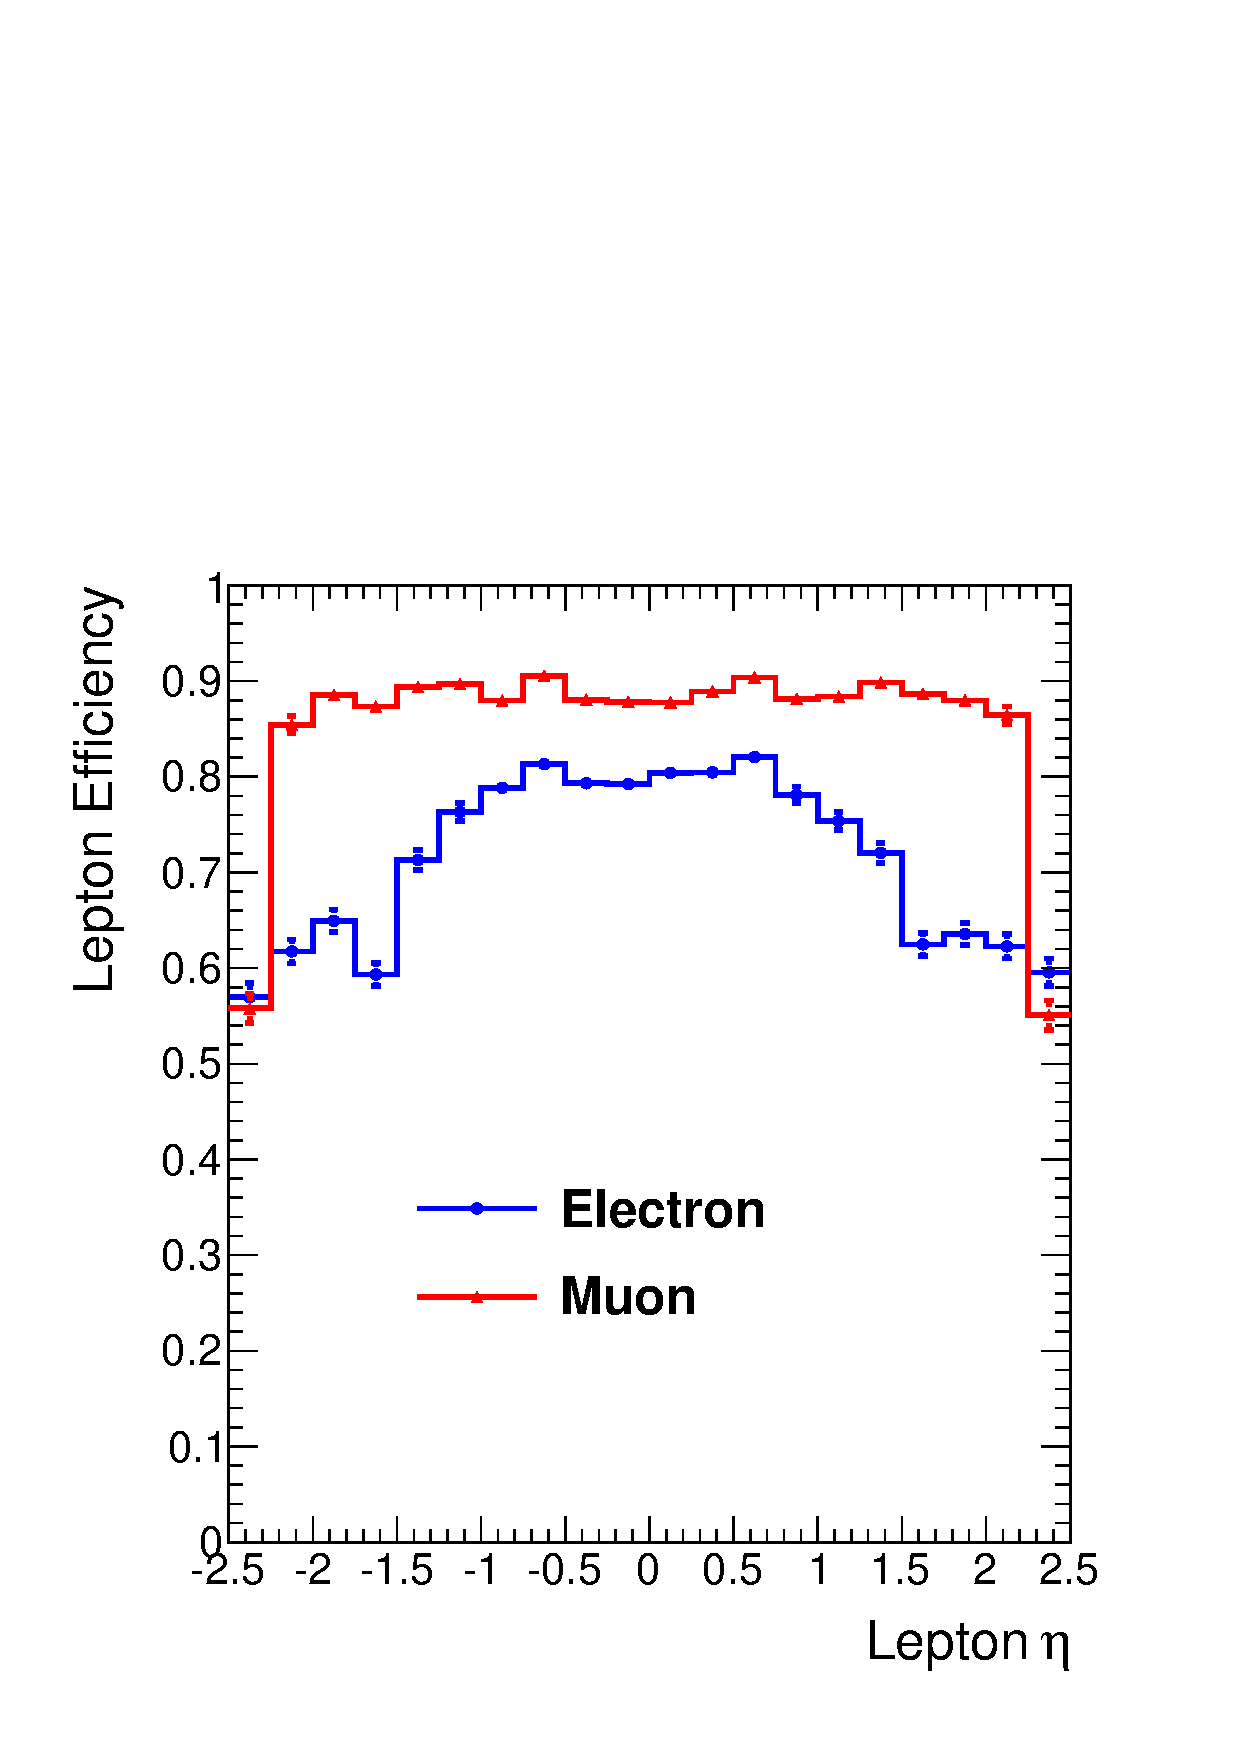
\includegraphics[width=0.4\textwidth]{figures/lepton_eff_Eta.pdf}
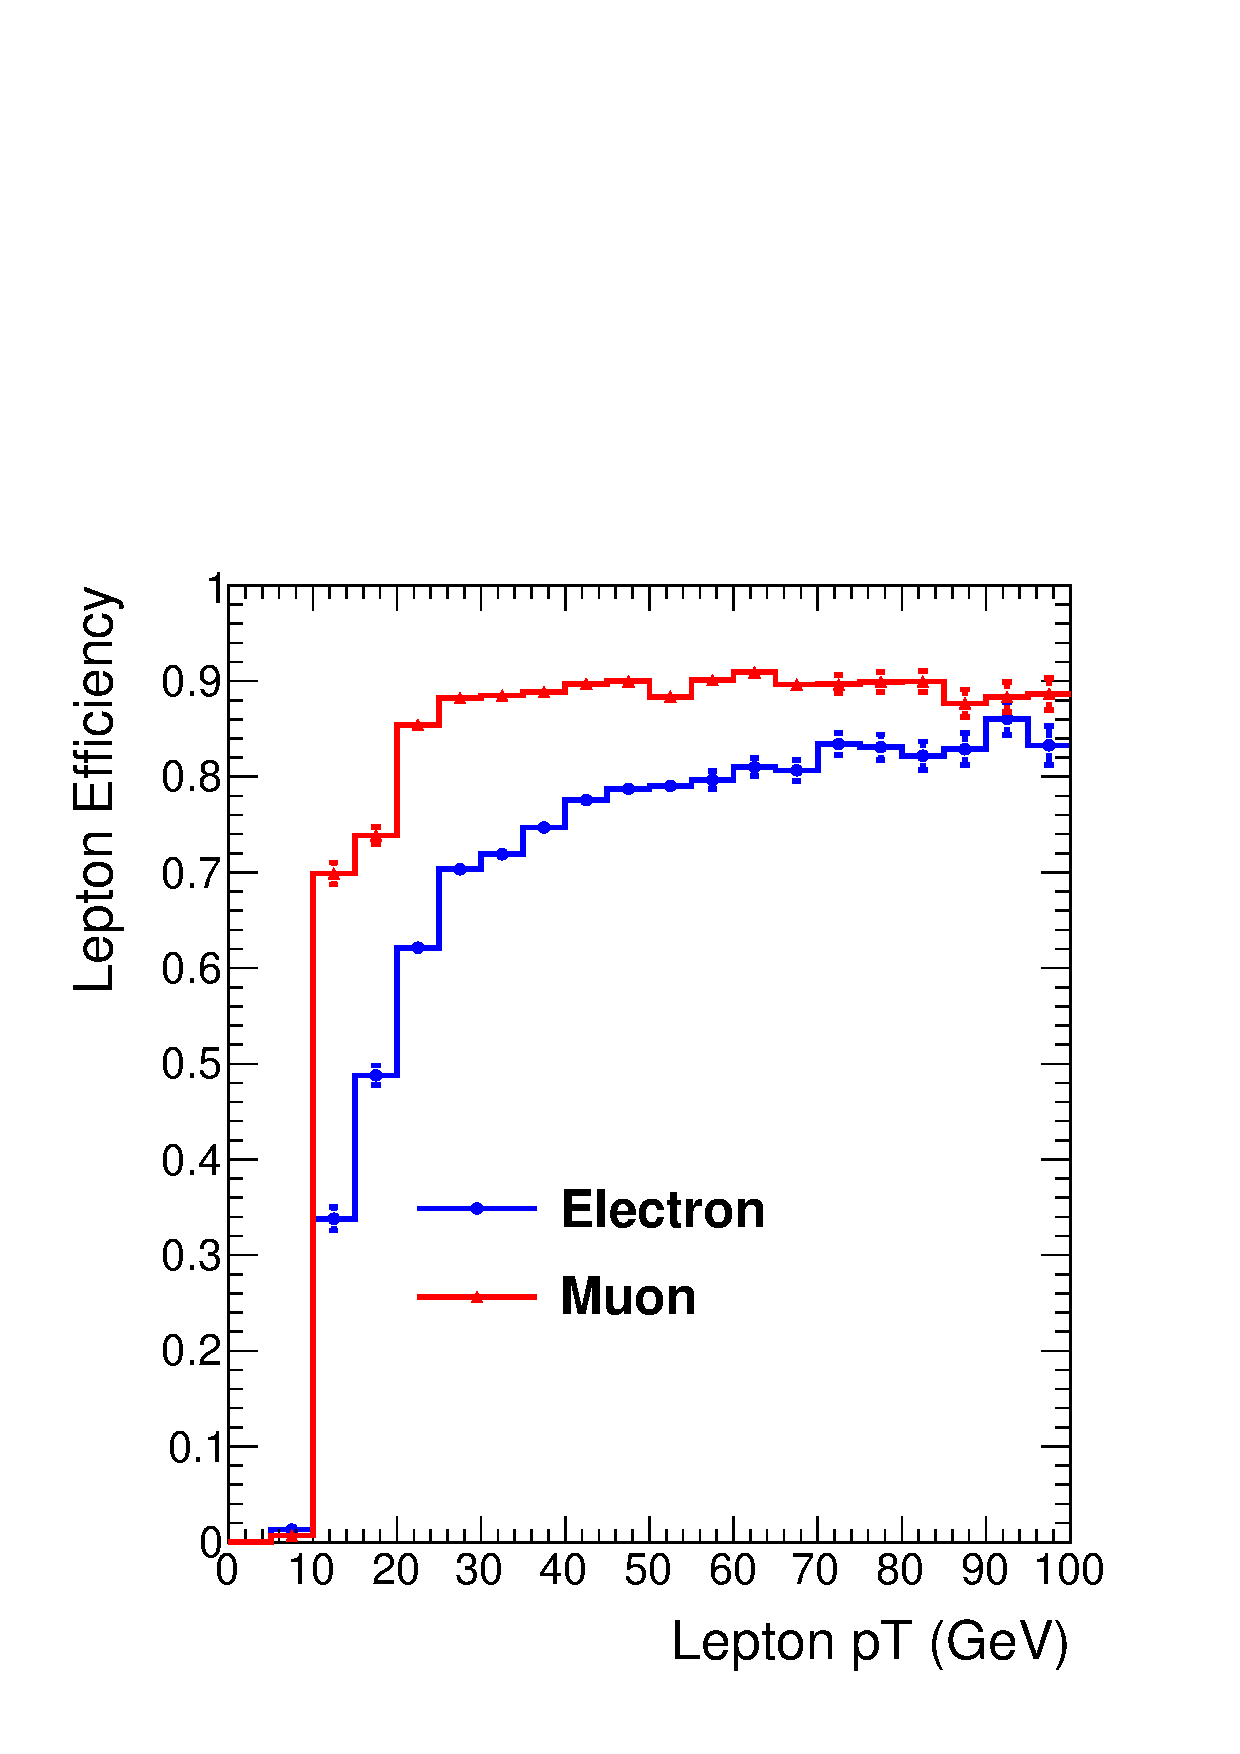
\includegraphics[width=0.4\textwidth]{figures/lepton_eff_Pt.pdf}\\
\caption{{\bf this needs to be updated for the ZZ sample, especially with the pT 30/20 selection..}Lepton efficiency as a function of the lepton $\eta$ (left) and $\pt$ (right) extracted 
from the $\ZZ$ Monte Carlo.}
\label{fig:lepeff_gen}
\end{center}
\end{figure}
%%%%%%%%%%%%%%%%%%%%%%%%%%%%%%


%\subsection{{\bf $k_T$} Function}
One final complication that must be considered is the boost of the initial state.
In the leading order Matrix Element calculation there is no initial state radiation. 
The initial state partons collide head-on and the system has no transverse boost. 
To account for the transverse recoil and thus improve the performance of our discriminant
on data, we integrate over the possible values of the system boost $k_{T}(k_{x},k_{y})$. 
The $k_T$ model is extracted from Monte Carlo for each process separately. 
Figure~\ref{fig:zzboost} shows the distribution of $k_T$ for $\hzz$ and 
the non-resonant $\ZZ$ processes.  


%%%%%%%%%%%%%%%%%%%%%%%%%%%%%%
\begin{figure}[!htbp]
\begin{center}
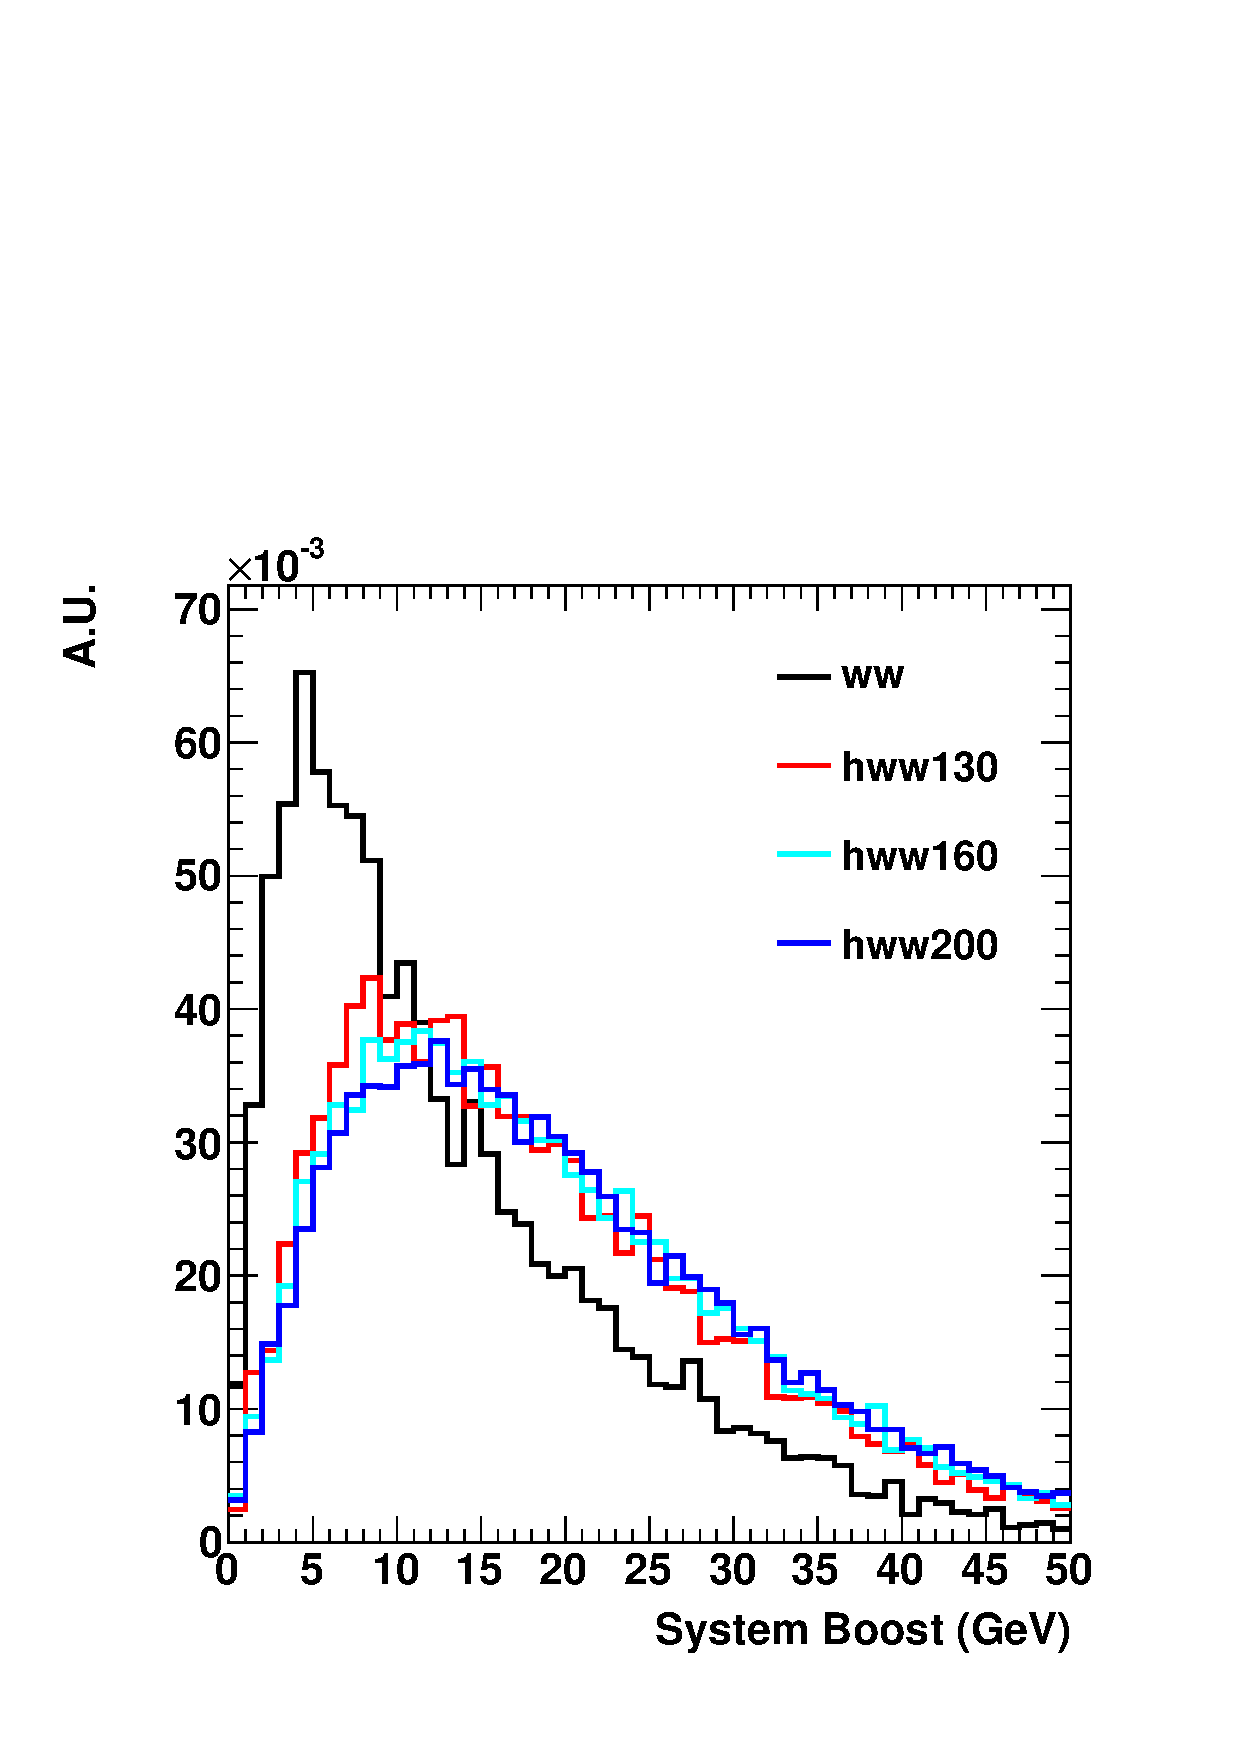
\includegraphics[width=0.5\textwidth]{figures/boost.pdf}
\caption{{\bf This needs to be replaced with the ones from hzz properly...}The transverse boost of the $WW$ system for $ZZ$ production and $\hzz$ at 3 different Higgs masses.}
\label{fig:zzboost}
\end{center}
\end{figure}
%%%%%%%%%%%%%%%%%%%%%%%%%%%%%%


\subsection{Likelihood Ratio Discriminator}
Event probabilities, calculated as described above, are used to construct 
a likelihood ratio discriminant which we use in a one-dimensional template fit.  
The discriminator is defined as :
\begin{equation}
\label{eqn:LR}
LR = \frac { P_s} { P_s + \sum_i k_{bi} P_{bi}},
\end{equation}
where $P_s$  is the probability for the signal, $P_{bi}$ is the probability for background
process $i$, and
$k_{bi}$ is the expected fractional contribution of background $i$,
satisfying the sum $\sum k_{bi} =1$.
Because signal events are expected to have $P_s>P_b$ and vice-versa for background events, 
the value of $LR$ is close to one for signal and zero for background processes.
The calculation of $P_s$ is a function of Higgs mass, so the likelihood ratio
shape depends on $m_H$. This is true for both signal and background templates of $LR$. 
Figure~\ref{fig:lrstacks} shows the likelihood ratio distributions for $m_H$~=~130, 160, and 200 $\GeVcc$, 
corresponding to 1~$\ifb$. 
Note that the backgrounds peak near $LR~=~0$ while the signal peaks near $LR~=~1$. 
%%%%%%%%%%%%%%%%%%%%%%%%%%%%%%
\begin{figure}[!hbtp]
\centering
\subfigure[]{
\centering
\label{subfig:lr_hm130}
%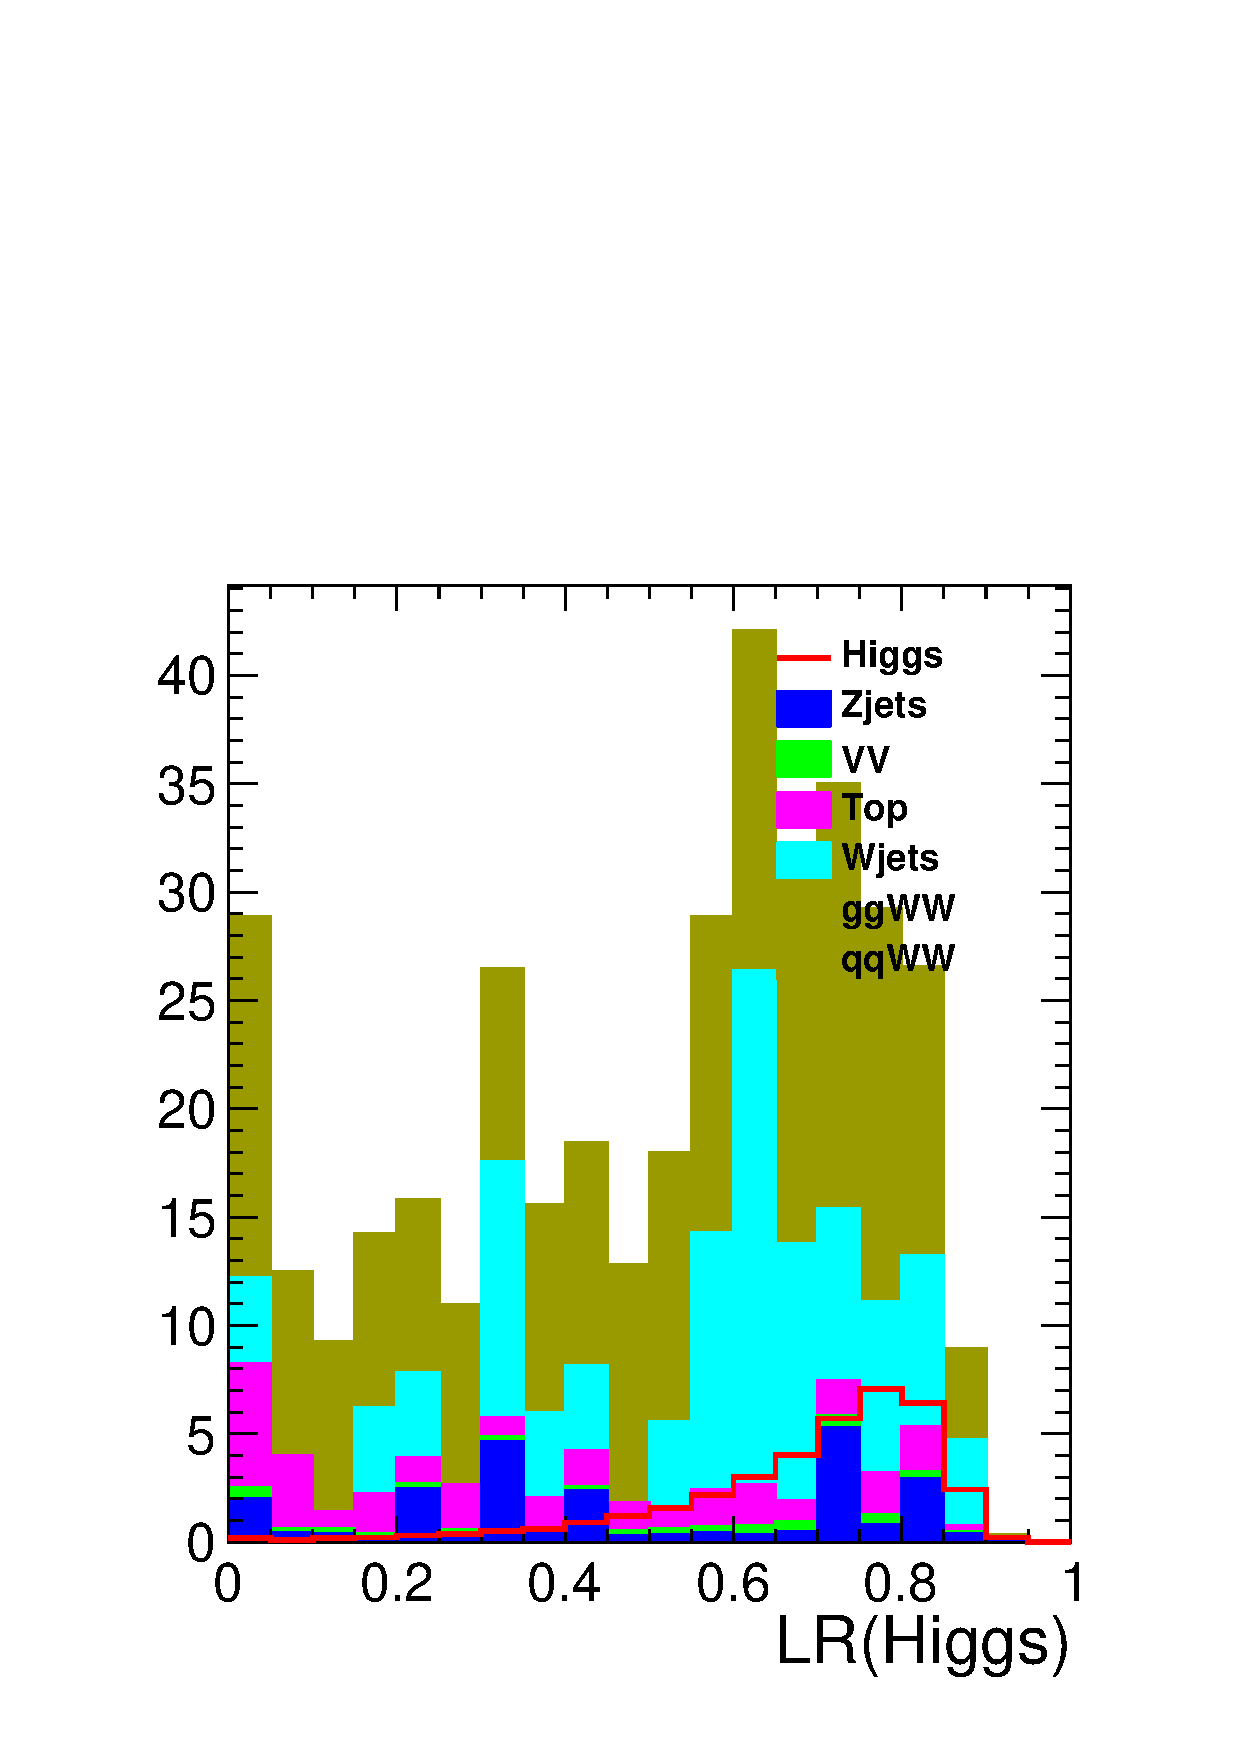
\includegraphics[width=.32\textwidth]{figures/hww130_LR.pdf}}
}
\caption{The matrix element output LR distribution after \ZZ\ pre-selection $m_H$=250 $\GeVcc$ 
\subref{subfig:lr_hm130} in the 0-jet bin.}
\label{fig:lrstacks}
\end{figure}
%%%%%%%%%%%%%%%%%%%%%%%%%%%%%%

It is important to note that because the $LR$ distribution is calculated the same way for data, 
signal and backgrounds, the fact that we use a LO Matrix Element and make certain 
approximations in the analytic calculation may result in less than optimal sensitivity 
but does not introduce any bias.

\subsection{Validation on the $\WZ/ZZ$ Cross-section Measurement}
We validate performance of our implementation of the Matrix Element technique by simultaneously measuring
$WZ$ and $ZZ$ cross-section in events with two-charged leptons and missing transverse energy.
 
After the preselection cuts, the only relevant background in the measurement is non-resonant $WW$ production.
Therefore, the main challenge is to discriminate $ZZ$ and $WZ$ events from $WW$.

In order to achieve this, we construct new Likelihood $LR_{ZZ+WZ}$, defined as:
\begin{equation}
\label{eqn:LRZZ}
LR_{ZZ+WZ} = \frac { P_{ZZ}+P_{WZ}} { P_{ZZ} + P_{WZ} + P_{WW} },
\end{equation}
where $P_{WZ}$ is evaluated with the assumption that two charged leptons originated from a $Z$-boson, while 
$W$ leptonically but the lepton was not reconstructed. Distribution of LR$_{ZZ+WZ}$ for data and predicted 
backgrounds and signal is shown in figure \ref{fig:lrzz}. One can see that shape of the  distribution in data is well 
modeled.

%%%%%%%%%%%%%%%%%%%%%%%%%%%%%%
\begin{figure}[!htbp]
\begin{center}
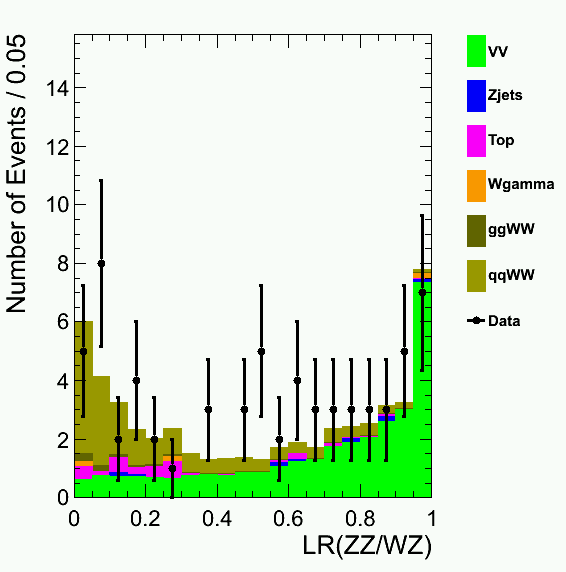
\includegraphics[width=0.5\textwidth]{figures/LRZZ.png}
\caption{$LR_{ZZ+WZ}$ in 1092 pb$^{-1}$ of data compared to expected backgrounds and $ZZ+WZ$ signal.}
\label{fig:lrzz}
\end{center}
\end{figure}
%%%%%%%%%%%%%%%%%%%%%%%%%%%%%%

Precise measurement of the cross-section requires clean sample of signal events. We, therefore, further select events
that pass $LR_{ZZ+WZ}>0.75$ requirement. Expected yields for each process as well as observed data count is shown in table \ref{tab:ZZWZselection}.

\begin{table}[!ht]
  \begin{center}
 {\scriptsize
  \begin{tabular} {|c|c|}
 \hline
  Process & Events \\
  \hline
  \hline
  $qq \rightarrow WW$   &  1.4 $\pm$   0.1 \\
  $gg \rightarrow WW$   &  0.1 $\pm$   0.01 \\
  $tt + tw$             &  0.15 $\pm$  0.05 \\
  $Z  + jets$           &  0.43 $\pm$  0.2 \\
  $W  + \gamma$          &  0.17 $\pm$  0.17 \\
  \hline
  Total Background      &  2.25 $\pm$  0.53 \\
  \hline
  $ZZ$                  &  11.5 $\pm$  0.2 \\
  $WZ$                  &  5.4  $\pm$  0.1 \\
 \hline
  Total Signal          &  16.9 $\pm$  0.3 \\
 \hline
  Data                  &  21               \\
 \hline
  \end{tabular}
  }
  \caption{Expected number of signal and background events for an 
  integrated luminosity of 1.092 \ifb{} after applying the $LR_{ZZ+WZ}>0.75$ requirements. 
 Monte Carlo statistical  uncertainties are included.}
   \label{tab:ZZWZselection}
  \end{center}
\end{table}
Assuming 100$\%$ systematic unceratanty on the backgrounds, we eastimate $ZZ+WZ$ cross-section to be 
$28.4 \pm 3.5$ pb, which is in good agreement with theoretical predictions.


 
%      \label{sec:sel_onejet}
%      The selection in the 1-jet bin starts from the strategy in the 0-jet bin with 
the addition of one reconstructed jet. To reject the bulk of the background, we 
require that the jet is not $b$-tagged and the angle between the dilepton 
system and the jet in the transverse plane must be smaller than 165 dg. for 
the $\mu\mu$ and $ee$ final states. The last cut rejects $\dyll$ events where 
the jet recoils against the $\Z$ boson.

The optimized selection requirements are shown for every mass hypothesis in 
Tab.~\ref{tab:cuts_analysis1j}. The expected number of signal and background 
events for an integrated luminosity of 1~$\ifb$, after applying the full 
cut based selection is shown in Table~\ref{tab:hwwselection1j}. The Higgs yield 
includes all processes, although the $gg \to H$ component is the dominant one by far.

\begin{table}[ht]
  \begin{center}
    \begin{tabular}{|c|c|c|c|c|c|}
    \hline
\mHi [GeV] & $\ptlmax$ [$\GeV$] & $\ptlmin$ [$\GeV$] & $\mll$ [$\GeV$] & $\delphill$ [dg.] & $m_{T}^{\ell\ell\met}$ [$\GeVcc$]  \\  \hline
           &   $>$               &   $>$               &   $<$             &  $<$          &	[,]			        \\  \hline
    120 & 20  &  20 & 40  & 60  & [20,120]\\
    130 & 25  &  20 & 45  & 60  & [20,130]\\
    140 & 25  &  20 & 45  & 60  & [20,140]\\
    150 & 27  &  25 & 50  & 60  & [20,150]\\
    160 & 30  &  25 & 50  & 60  & [20,160]\\
    170 & 34  &  25 & 50  & 60  & [20,170]\\
    180 & 36  &  25 & 60  & 70  & [20,180]\\
    190 & 38  &  25 & 80  & 90  & [20,190]\\
    200 & 40  &  25 & 90  & 100 & [20,200]\\
    250 & 55  &  25 & 150 & 140 & [20,250]\\
    300 & 70  &  25 & 200 & 175 & [20,300]\\
    350 & 80  &  25 & 250 & 175 & [20,350]\\
    400 & 90  &  25 & 300 & 175 & [20,400]\\
    450 & 110 &  25 & 350 & 175 & [20,450]\\
    500 & 120 &  25 & 400 & 175 & [20,500]\\
    550 & 130 &  25 & 450 & 175 & [20,550]\\
    600 & 140 &  25 & 500 & 175 & [20,600]\\
      \hline
    \end{tabular}
  \end{center}
  \caption{Optimized selection cuts for different mass hypotheses for the 1-jet bin case.}
  \label{tab:cuts_analysis1j}
\end{table}

\begin{table}[!ht]
  \begin{center}
 {\footnotesize
  \begin{tabular} {|c|c|c|c|c|c|c|c|}
\hline
  mass    & SM $H\to WW$ & all bkg. & $qq \to \WW$ & $gg \to \WW$ & all non-$\WW$ bkg. \\
  \hline
  \hline
120 &  3.57 $\pm$  0.11 &  22.65 $\pm$  3.36 &  9.55 $\pm$  0.32 & 0.54 $\pm$  0.01 & 12.56 $\pm$  3.34 \\
130 &  7.79 $\pm$  0.23 &  28.32 $\pm$  3.38 & 12.95 $\pm$  0.38 & 0.79 $\pm$  0.04 & 14.58 $\pm$  3.35 \\
140 & 13.10 $\pm$  0.39 &  32.16 $\pm$  3.41 & 14.93 $\pm$  0.41 & 1.00 $\pm$  0.05 & 16.23 $\pm$  3.38 \\
150 & 20.10 $\pm$  0.60 &  42.31 $\pm$  3.28 & 19.58 $\pm$  0.46 & 1.39 $\pm$  0.06 & 21.34 $\pm$  3.24 \\
160 & 19.53 $\pm$  0.59 &  15.79 $\pm$  0.54 &  8.85 $\pm$  0.31 & 0.80 $\pm$  0.04 &  6.14 $\pm$  0.44 \\
170 & 16.01 $\pm$  0.48 &  15.74 $\pm$  0.50 &  8.34 $\pm$  0.17 & 0.80 $\pm$  0.04 &  6.60 $\pm$  0.46 \\
180 & 14.23 $\pm$  0.43 &  23.45 $\pm$  0.74 & 11.70 $\pm$  0.20 & 1.06 $\pm$  0.03 & 10.69 $\pm$  0.71 \\
190 & 12.61 $\pm$  0.38 &  44.54 $\pm$  4.28 & 19.71 $\pm$  0.41 & 1.47 $\pm$  0.03 & 23.36 $\pm$  4.26 \\
200 &  9.94 $\pm$  0.30 &  48.97 $\pm$  4.18 & 21.27 $\pm$  0.43 & 1.53 $\pm$  0.03 & 26.17 $\pm$  4.15 \\
250 &  6.09 $\pm$  0.18 &  57.88 $\pm$  4.19 & 24.65 $\pm$  0.46 & 1.37 $\pm$  0.03 & 31.86 $\pm$  4.16 \\
300 &  4.84 $\pm$  0.15 &  47.13 $\pm$  4.19 & 19.60 $\pm$  0.21 & 0.91 $\pm$  0.04 & 26.62 $\pm$  4.18 \\
350 &  4.61 $\pm$  0.14 &  40.20 $\pm$  4.14 & 16.49 $\pm$  0.38 & 0.76 $\pm$  0.03 & 22.95 $\pm$  4.12 \\
400 &  3.82 $\pm$  0.11 &  36.12 $\pm$  4.48 & 13.12 $\pm$  0.38 & 0.61 $\pm$  0.03 & 22.39 $\pm$  4.46 \\
450 &  2.18 $\pm$  0.07 &  19.36 $\pm$  2.23 &  7.40 $\pm$  0.25 & 0.37 $\pm$  0.02 & 11.59 $\pm$  2.21 \\
500 &  1.43 $\pm$  0.04 &  14.67 $\pm$  2.11 &  5.84 $\pm$  0.22 & 0.31 $\pm$  0.00 &  8.52 $\pm$  2.09 \\
500 &  0.91 $\pm$  0.03 &  10.94 $\pm$  1.66 &  4.78 $\pm$  0.13 & 0.24 $\pm$  0.00 &  5.92 $\pm$  1.65 \\
600 &  0.58 $\pm$  0.02 &   9.45 $\pm$  1.59 &  3.80 $\pm$  0.11 & 0.19 $\pm$  0.00 &  5.46 $\pm$  1.58 \\
 \hline
  \end{tabular}
  }
 {\small
  \begin{tabular} {|c|c|c|c|c|}
\hline
  mass    & $\ttbar+tW$ & non-resonant $WZ$/$ZZ$ & $\dyll+WZ+ZZ$ & $\Wjets/\gamma$ \\
  \hline
  \hline
120 &  6.26 $\pm$  0.99 & 0.95 $\pm$  0.11 &  2.26 $\pm$  0.78 & 3.09 $\pm$  3.09  \\
130 &  8.07 $\pm$  1.03 & 1.08 $\pm$  0.11 &  2.33 $\pm$  0.78 & 3.09 $\pm$  3.09  \\
140 &  9.59 $\pm$  1.13 & 1.18 $\pm$  0.12 &  2.36 $\pm$  0.78 & 3.09 $\pm$  3.09  \\
150 & 14.49 $\pm$  0.57 & 1.37 $\pm$  0.13 &  2.39 $\pm$  0.78 & 3.09 $\pm$  3.09  \\
160 &  5.22 $\pm$  0.32 & 0.49 $\pm$  0.08 &  0.43 $\pm$  0.30 & 0.00 $\pm$  0.00  \\
170 &  5.78 $\pm$  0.35 & 0.38 $\pm$  0.07 &  0.42 $\pm$  0.30 & 0.00 $\pm$  0.00  \\
180 &  8.38 $\pm$  0.43 & 0.55 $\pm$  0.08 &  1.76 $\pm$  0.56 & 0.00 $\pm$  0.00  \\
190 & 14.88 $\pm$  1.54 & 1.03 $\pm$  0.11 &  3.74 $\pm$  1.42 & 3.70 $\pm$  3.70  \\
200 & 17.52 $\pm$  1.24 & 1.17 $\pm$  0.07 &  3.76 $\pm$  1.42 & 3.70 $\pm$  3.70  \\
250 & 24.01 $\pm$  1.39 & 1.34 $\pm$  0.09 &  2.77 $\pm$  1.18 & 3.74 $\pm$  3.74  \\
300 & 19.99 $\pm$  1.76 & 0.95 $\pm$  0.07 &  1.94 $\pm$  0.68 & 3.74 $\pm$  3.74  \\
350 & 17.21 $\pm$  1.67 & 0.72 $\pm$  0.04 &  1.27 $\pm$  0.54 & 3.74 $\pm$  3.74  \\
400 & 15.46 $\pm$  1.60 & 0.52 $\pm$  0.03 &  2.65 $\pm$  1.85 & 3.74 $\pm$  3.74  \\
450 &  8.85 $\pm$  1.21 & 0.18 $\pm$  0.02 &  2.55 $\pm$  1.85 & 0.00 $\pm$  0.00  \\
500 &  5.85 $\pm$  0.98 & 0.17 $\pm$  0.05 &  2.51 $\pm$  1.85 & 0.00 $\pm$  0.00  \\
500 &  4.30 $\pm$  0.84 & 0.12 $\pm$  0.02 &  1.50 $\pm$  1.43 & 0.00 $\pm$  0.00  \\
600 &  3.89 $\pm$  0.70 & 0.09 $\pm$  0.02 &  1.47 $\pm$  1.43 & 0.00 $\pm$  0.00  \\
  \hline
  \hline

 \hline
  \end{tabular}
  }
  \caption{Expected number of signal and background events for an 
  integrated luminosity of 1 $\ifb$, after applying the full cut based 
  selection in the 1-jet bin case. Monte Carlo statistical uncertainties are included.}
   \label{tab:hwwselection1j}
  \end{center}
\end{table}

%    \subsubsection{VBF Selection}
%      \label{sec:sel_vbf}
%      The cross section for Higgs boson production in the vector boson fusion (VBF)
mode is roughly ten times smaller than the gluon-gluon fusion mode.
However, the VBF signal can be extracted
using simple selections, especially in the fully leptonic decay channel
where the backgrounds are expected to be relatively low.

The $\hww$ events from VBF production is characterized by a pair of energetic 
forward-backward jets and very little hadronic activity in the rest of the event. 
As a starting point, we select the events that pass the $\ww$ preselection 
requiring two reconstructed jets with $\pt~>~30~\GeV$ and no other jets between 
them with $\pt~>~30~\GeV$. To reject the main background from top decays we 
apply further selections on the two jets $j_1$ and $j_2$:
\begin{itemize}
  \item neither of the jets must be $b$-tagged;
  \item $\Delta\eta (j_1-j_2) > 3.5$;
  \item $m_{j_1j_2} > 450\:\GeV$;
  \item $30~\GeV < m_{T}^{\ell\ell\met} < m_H~\GeV$.
\end{itemize}
To improve the selection efficiency signal we select 
events with a $\mHi$ dependent requirement on the high end of the dilepton mass 
(the actual cut value is the same as in the MVA analysis, 
see Sec.~\ref{sec:anal_mva}, Table~\ref{tab:presel_tmva_analysis}). 
Events with same and opposite flavor final states 
are separated in order to obtain better sensitivity in the final limit.   
The $qqH$ contribution to the total  $\hww$ signal is found to be about 85\%
after full event selections for all the mass hypotheses considered. 

%  \subsection{MVA Analysis}
%    \label{sec:anal_mva}
%    To make maximal use of the event information we have performed a multivariate analysis 
using a multivariate classifier based on the Boosted Decision Tree (BDT) technique. 
The BDT is implemented using the TMVA~\cite{tmva} toolkit and has been 
successfully applied in high energy physics to increase the 
statistical significance of a signal extraction
It requires less training than other multivariate classifiers and 
it is insensitive to the inclusion of poorly discriminating input variables.

%Just as other multivariate technique (like artificial neural networks, likelihood estimators, 
%k-Nearest Neighbor classifiers, etc..) that has been already successfully applied 
%in high energy physics to increase the statistical significance of a signal 
%extraction. 

In addition to the $\WW$ preselection, we apply a loose cut on the
maximum $\mll$ to enhance the signal-to-background ratio shown in Table~\ref{tab:presel_tmva_analysis}. 
The multivariate technique uses the following additional variables compared to the cut-based analysis: 
\begin{itemize}
\item $\Delta R_{\Lep\Lep}\equiv\sqrt{\deletall^2 + \delphill^2}$ between the leptons, 
with $\deletall$ the $\eta$ difference between the leptons, 
which has similar properties as $\delphill$
\item the angle in the transverse plane between 
the $\met$ and the leptons, which discriminates against events with 
no real $\met$
\item the {\it projected $\met$}
\item the transverse mass of both lepton-\met pairs, $m_T^{\ell-\met}$, which 
helps in reducing the non-$\W$ background
\item lepton flavors ($\mu\mu$, $ee$, $e\mu$ or $\mu e$ ). 
\end{itemize}
%These variables either have 
%large correlations with the previous ones or they do not give a large separation 
%power by themselves. Nevertheless they improve the overall performance. For the 
%current version of the analysis only two variables have been added:

The training has been carried out separately in the 0-jet and 1-jet bins 
for different Higgs masses using the corresponding signal samples. 
The classifier outputs for three different Higgs masses and both jet bins are shown in 
Figures~\ref{fig:histo_mva_130}-\ref{fig:histo_mva_200}. 

The cut on the BDT output has been chosen to maximize 
the statistical significance $S$ defined as:
\begin{equation*}
S=\frac{N_S}{\sqrt{N_B+(\Delta N_B)^2}}
\end{equation*}
where $N_S$ and $N_B$ are the expected signal and background event yields, 
assuming the SM cross-sections and 1 $\ifb$ of integrated luminosity. 
Exclusively for the cuts optimization, the relative uncertainty 
$\Delta N_B/N_B$ on the combined background is considered to be equal to 35\%. 
This is just a rough estimation of the overall uncertainty. We have tested 
other values between 20\% and 50\% and obtained consistent results.
The expected number of signal and background events for an integrated luminosity 
of 1 $\ifb$, after applying the full multivariate analysis selection in the 0-jet and 1-jet 
bin cases are listed in Tables~\ref{tab:mvasel0j} and ~\ref{tab:mvasel1j}, respectively.

\begin{table}
\begin{center}
\begin{tabular}{|r|c|c|c|c|c|c|c|c|c|c|c|c|}
\hline
$\mHi~~~~~[\GeV]$   & 120 & 130 & 140 & 150 & 160 & 170 & 180 & 190 & 200 & 210 \\
\hline
$\mll<~~~[\GeV]$    &  70 &  80 &  90 & 100 & 100 & 100 & 110 & 120 & 130 & 140 \\
\hline
\end{tabular}
%\vspace{0.5cm}
\begin{tabular}{|r|c|c|c|c|c|c|c|c|c|c|c|}
\hline
$\mHi~~~~~[\GeV]$    & 220 & 230 & 250 & 300 & 350 & 400 & 450 & 500 & 550 & 600 \\
\hline
$\mll<~~~[\GeV]$     & 150 & 230 & 250 & 300 & 350 & 400 & 450 & 500 & 550 & 600 \\
\hline
\end{tabular}
\caption{$\mll$ upper limit requirement as a function of the Higgs mass used to 
enrich the background datasets of signal-like events. These samples are employed 
in the training of the multivariate classifier used for the signal 
extraction.\label{tab:presel_tmva_analysis}}
\end{center}
\end{table}

\begin{figure}[!ht]
\begin{center}
   \subfigure[]{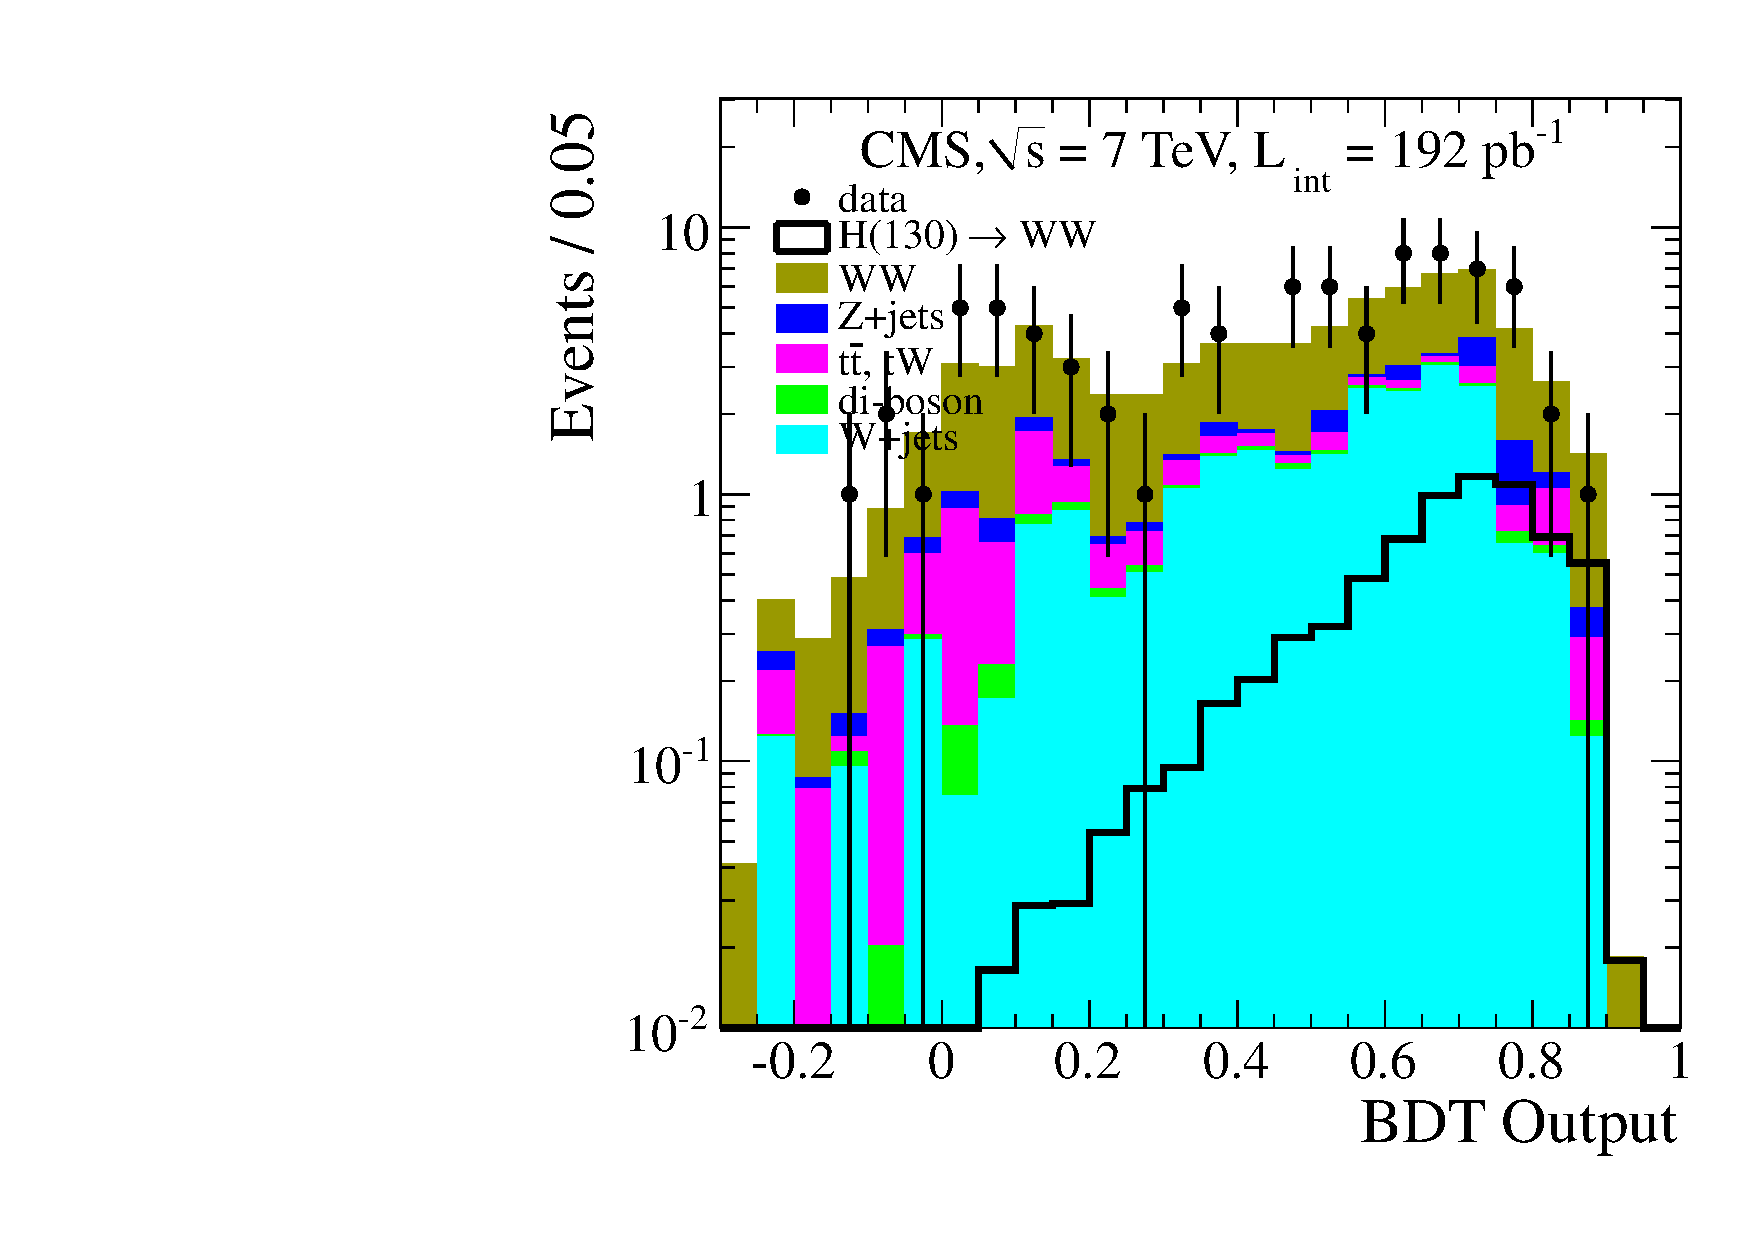
\includegraphics[width=0.49\textwidth,angle=0]{figures/histo_mva_130_0j.pdf}} 
   \subfigure[]{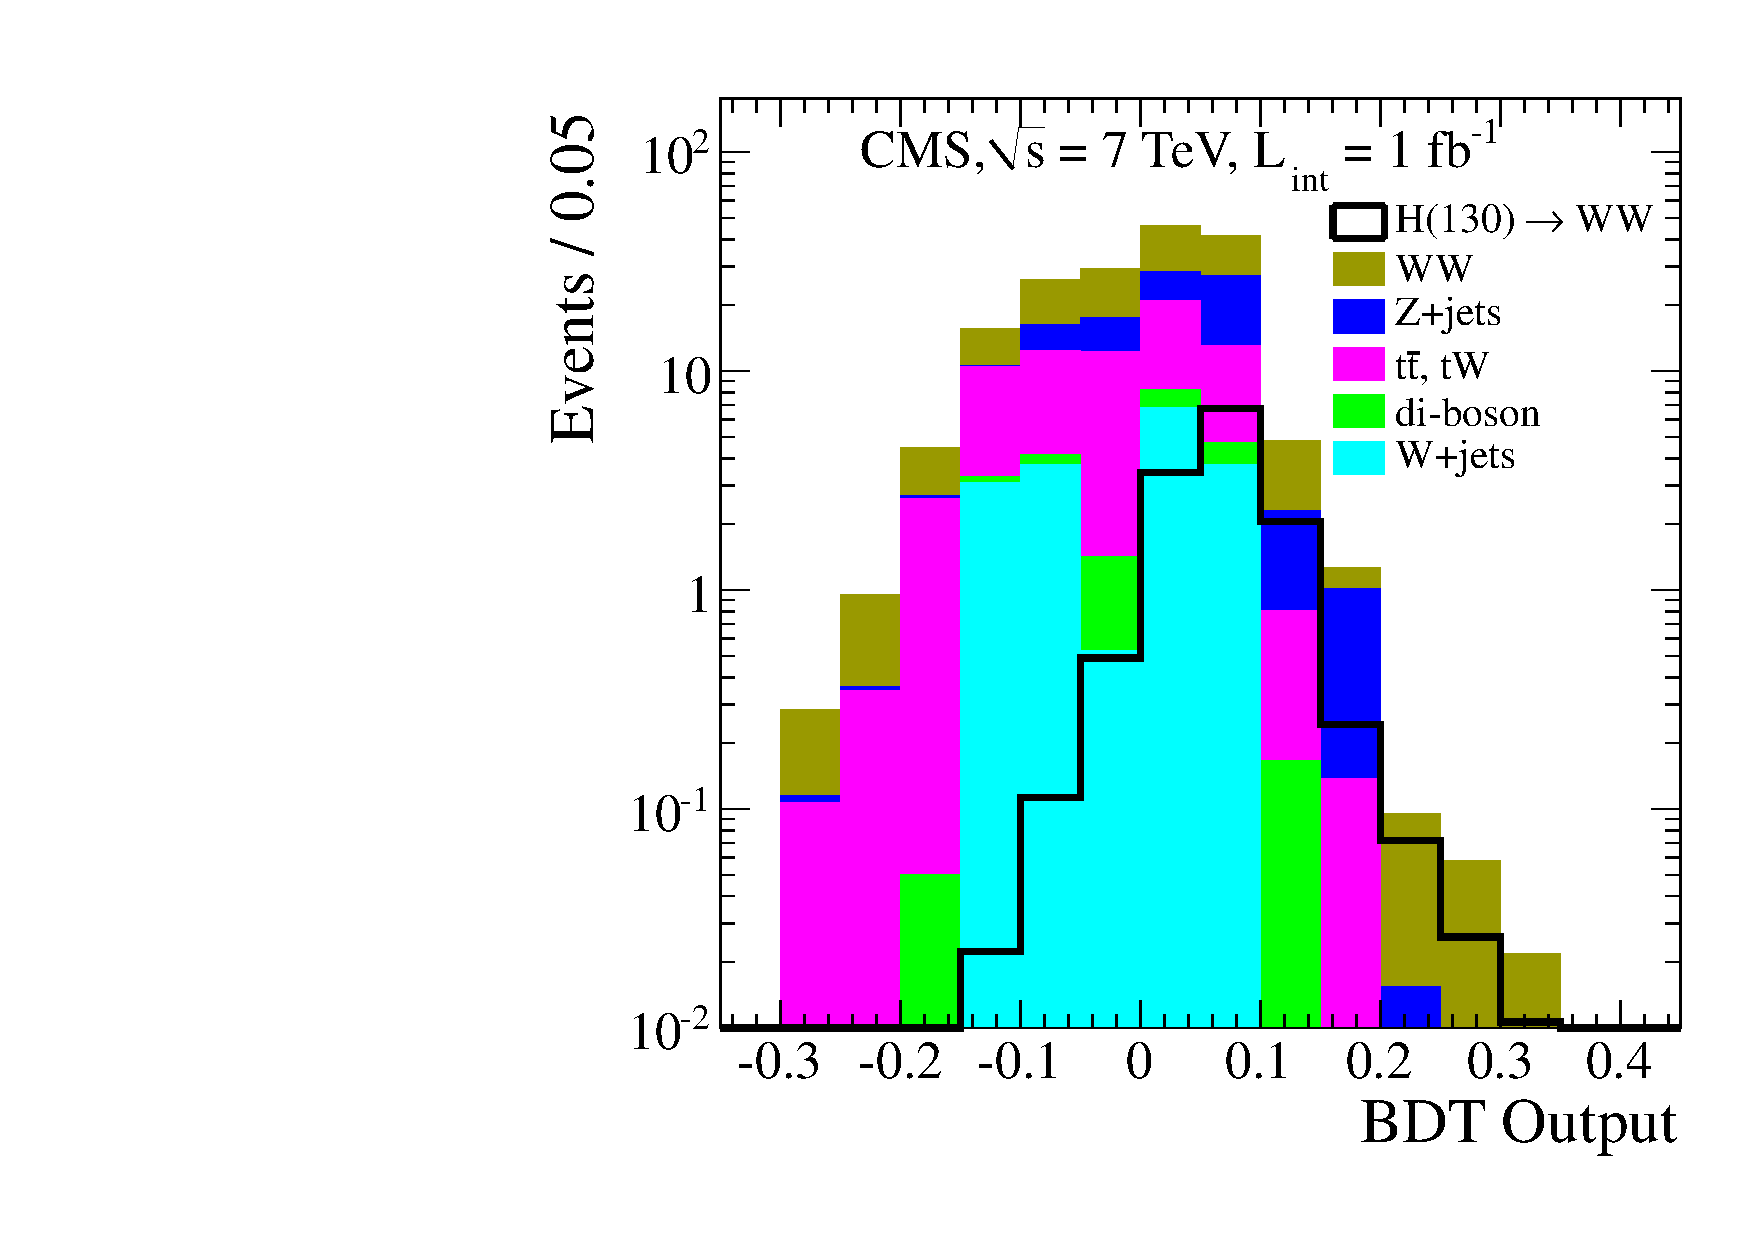
\includegraphics[width=0.49\textwidth,angle=0]{figures/histo_mva_130_1j.pdf}} 
       \caption{Classifier outputs for Higgs signal and background events 
for \mHi=130 $\GeVcc$ in the 0-jet bin (a) and 1-jet bin (b) after the $\WW$ selection. The number 
of events is different on each mass point due to the specific $\mll$ requirement.}
   \label{fig:histo_mva_130}
\end{center}
\end{figure}

\begin{figure}[!ht]
\begin{center}
   \subfigure[]{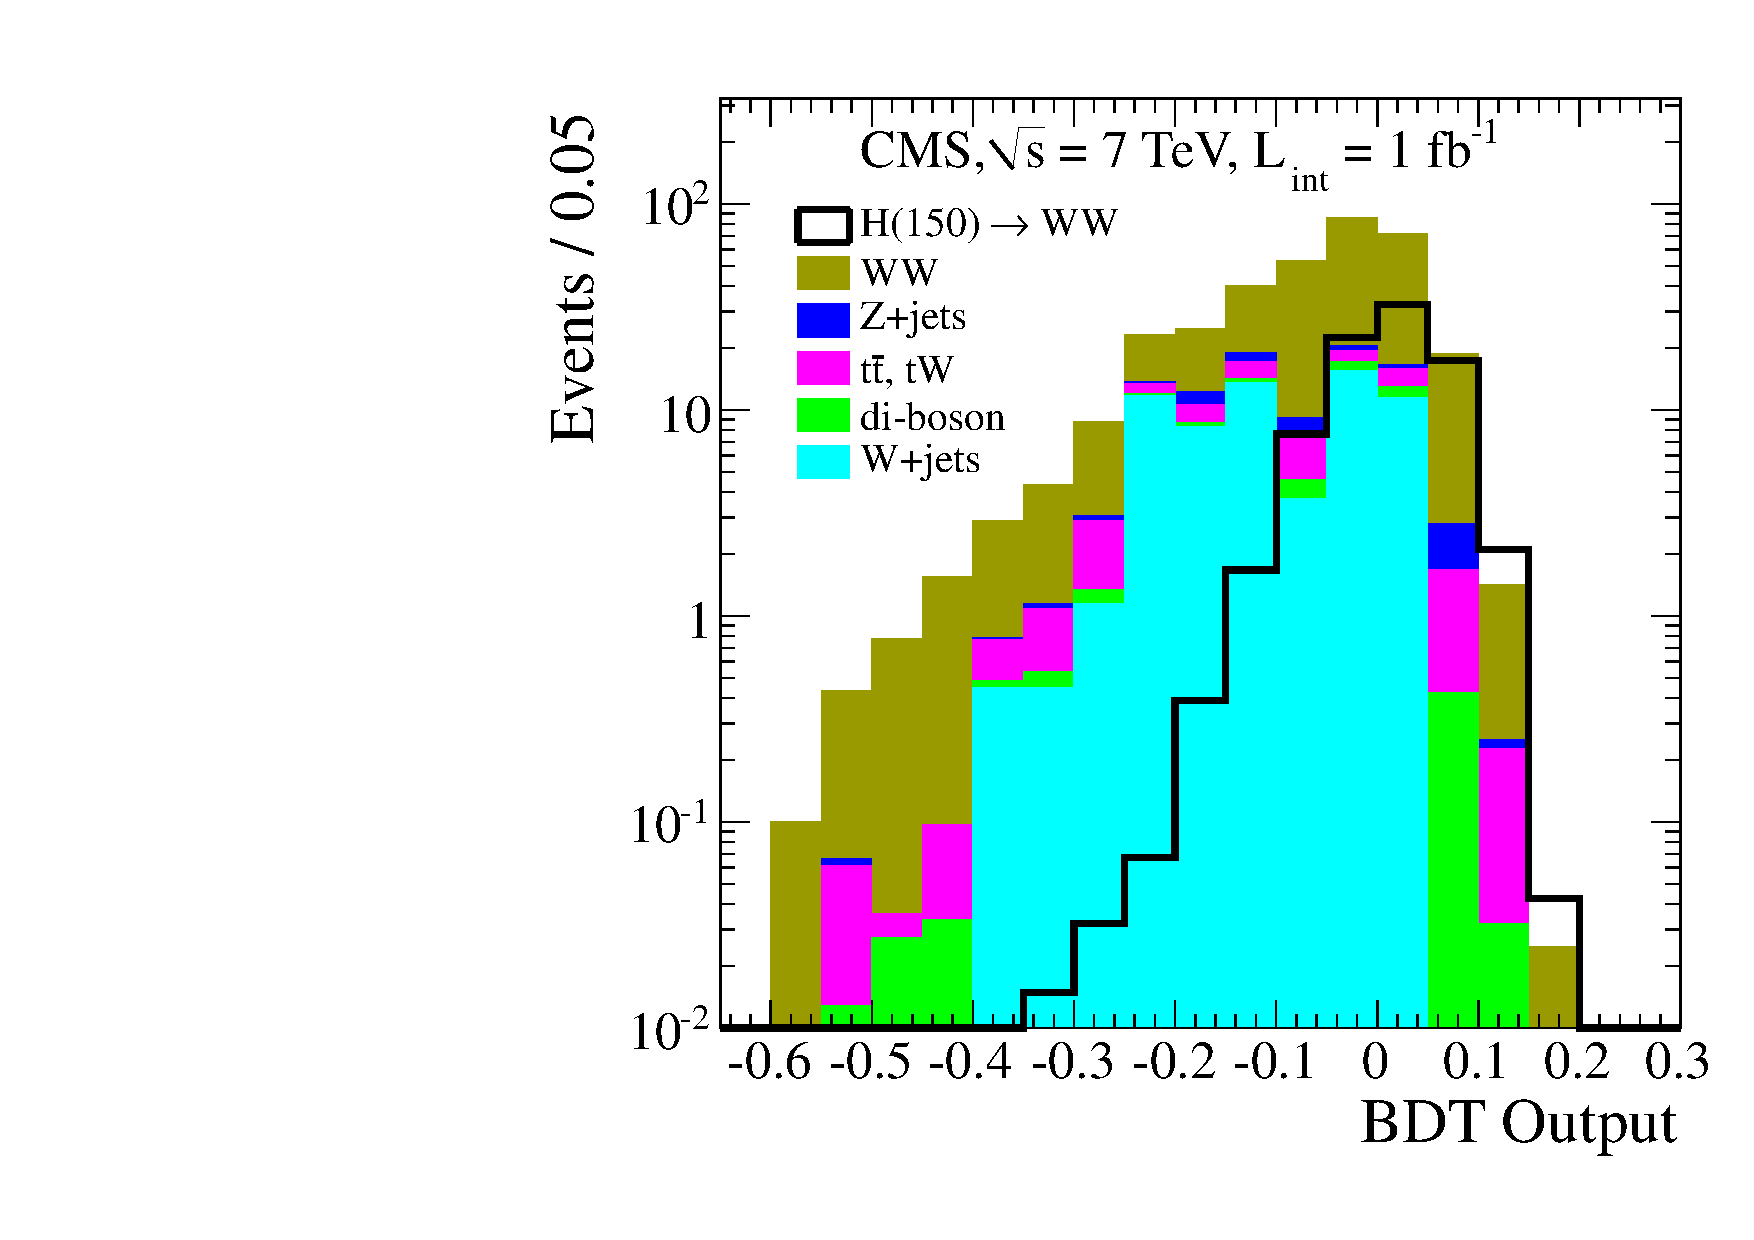
\includegraphics[width=0.49\textwidth,angle=0]{figures/histo_mva_150_0j.pdf}} 
   \subfigure[]{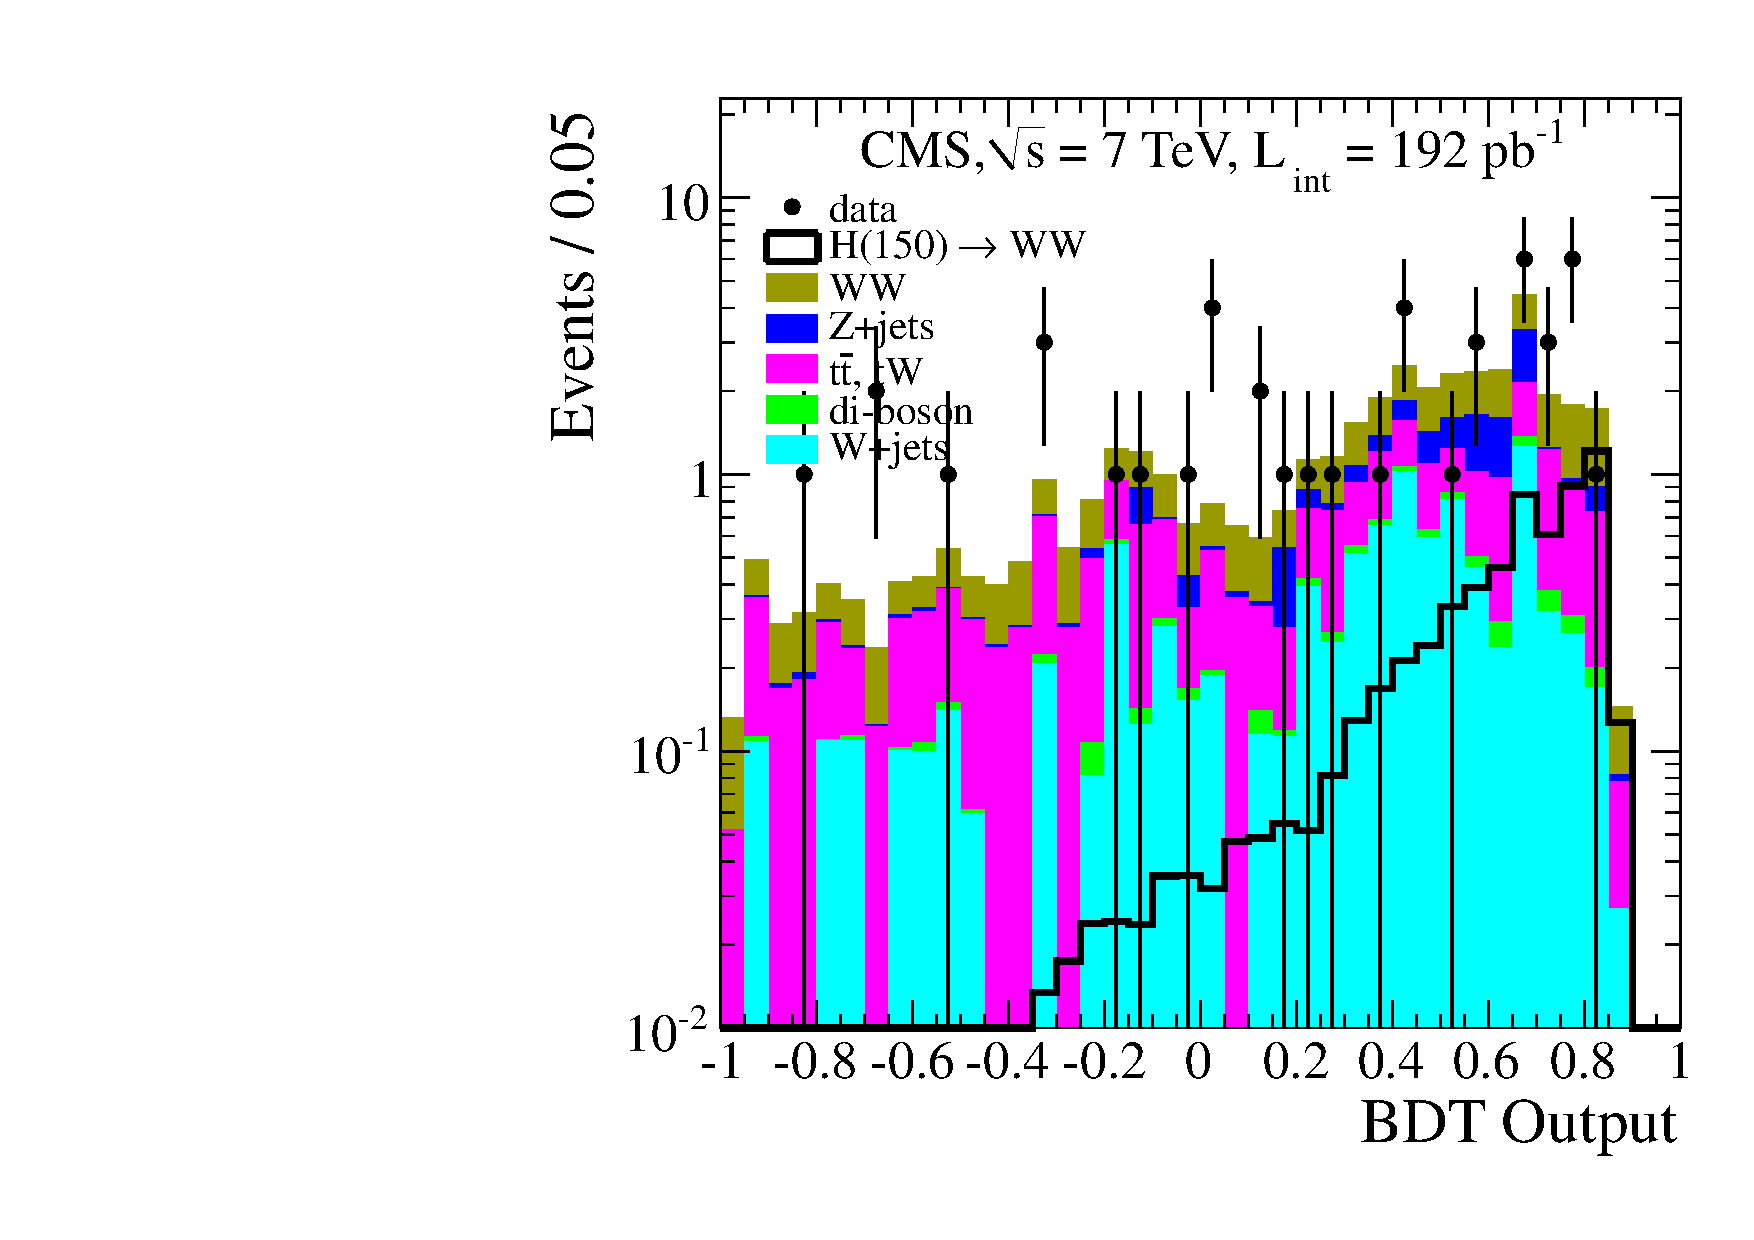
\includegraphics[width=0.49\textwidth,angle=0]{figures/histo_mva_150_1j.pdf}} 
       \caption{Classifier outputs for Higgs signal and background events 
for \mHi=150 $\GeVcc$ in the 0-jet bin (a) and 1-jet bin (b) after the $\WW$ selection. The number 
of events is different on each mass point due to the specific $\mll$ requirement.}
   \label{fig:histo_mva_150}
\end{center}
\end{figure}

\begin{figure}[!ht]
\begin{center}
   \subfigure[]{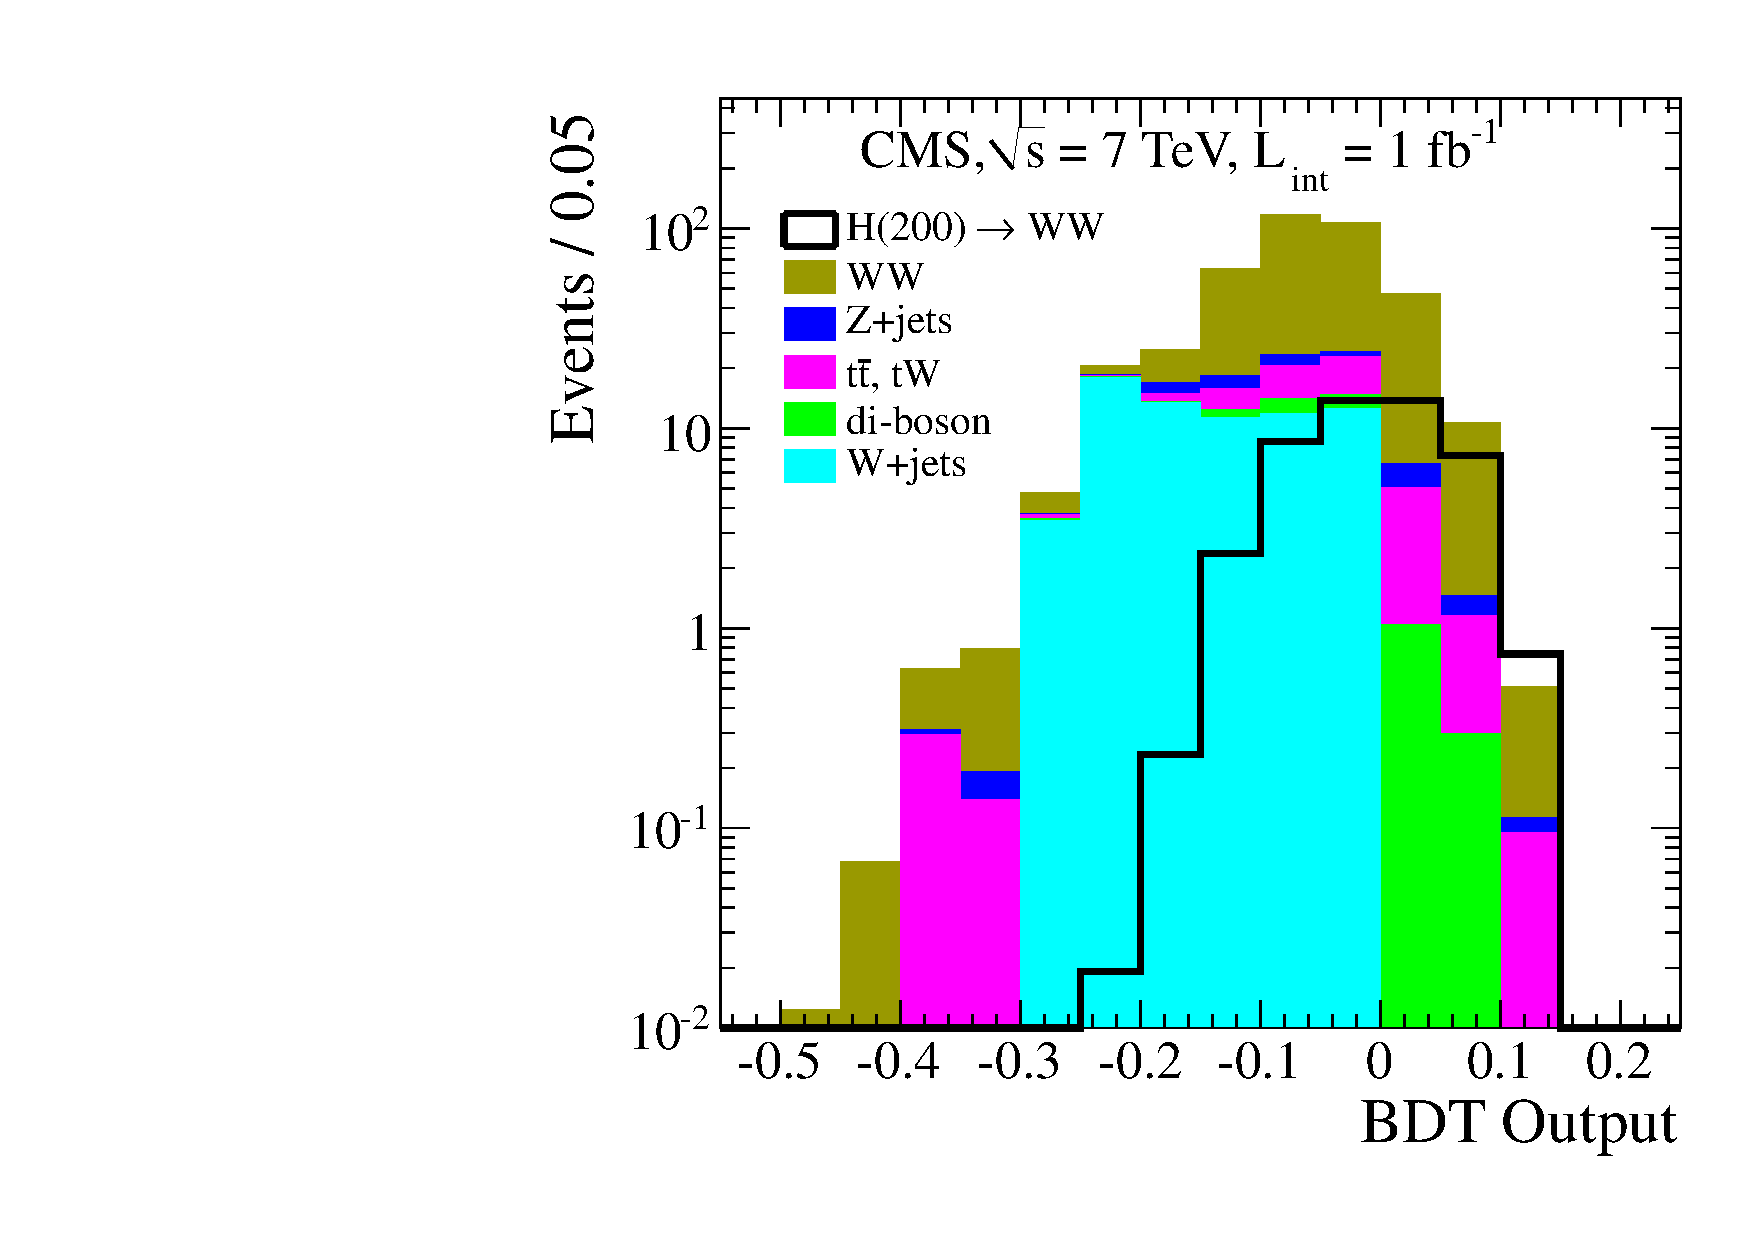
\includegraphics[width=0.49\textwidth,angle=0]{figures/histo_mva_200_0j.pdf}} 
   \subfigure[]{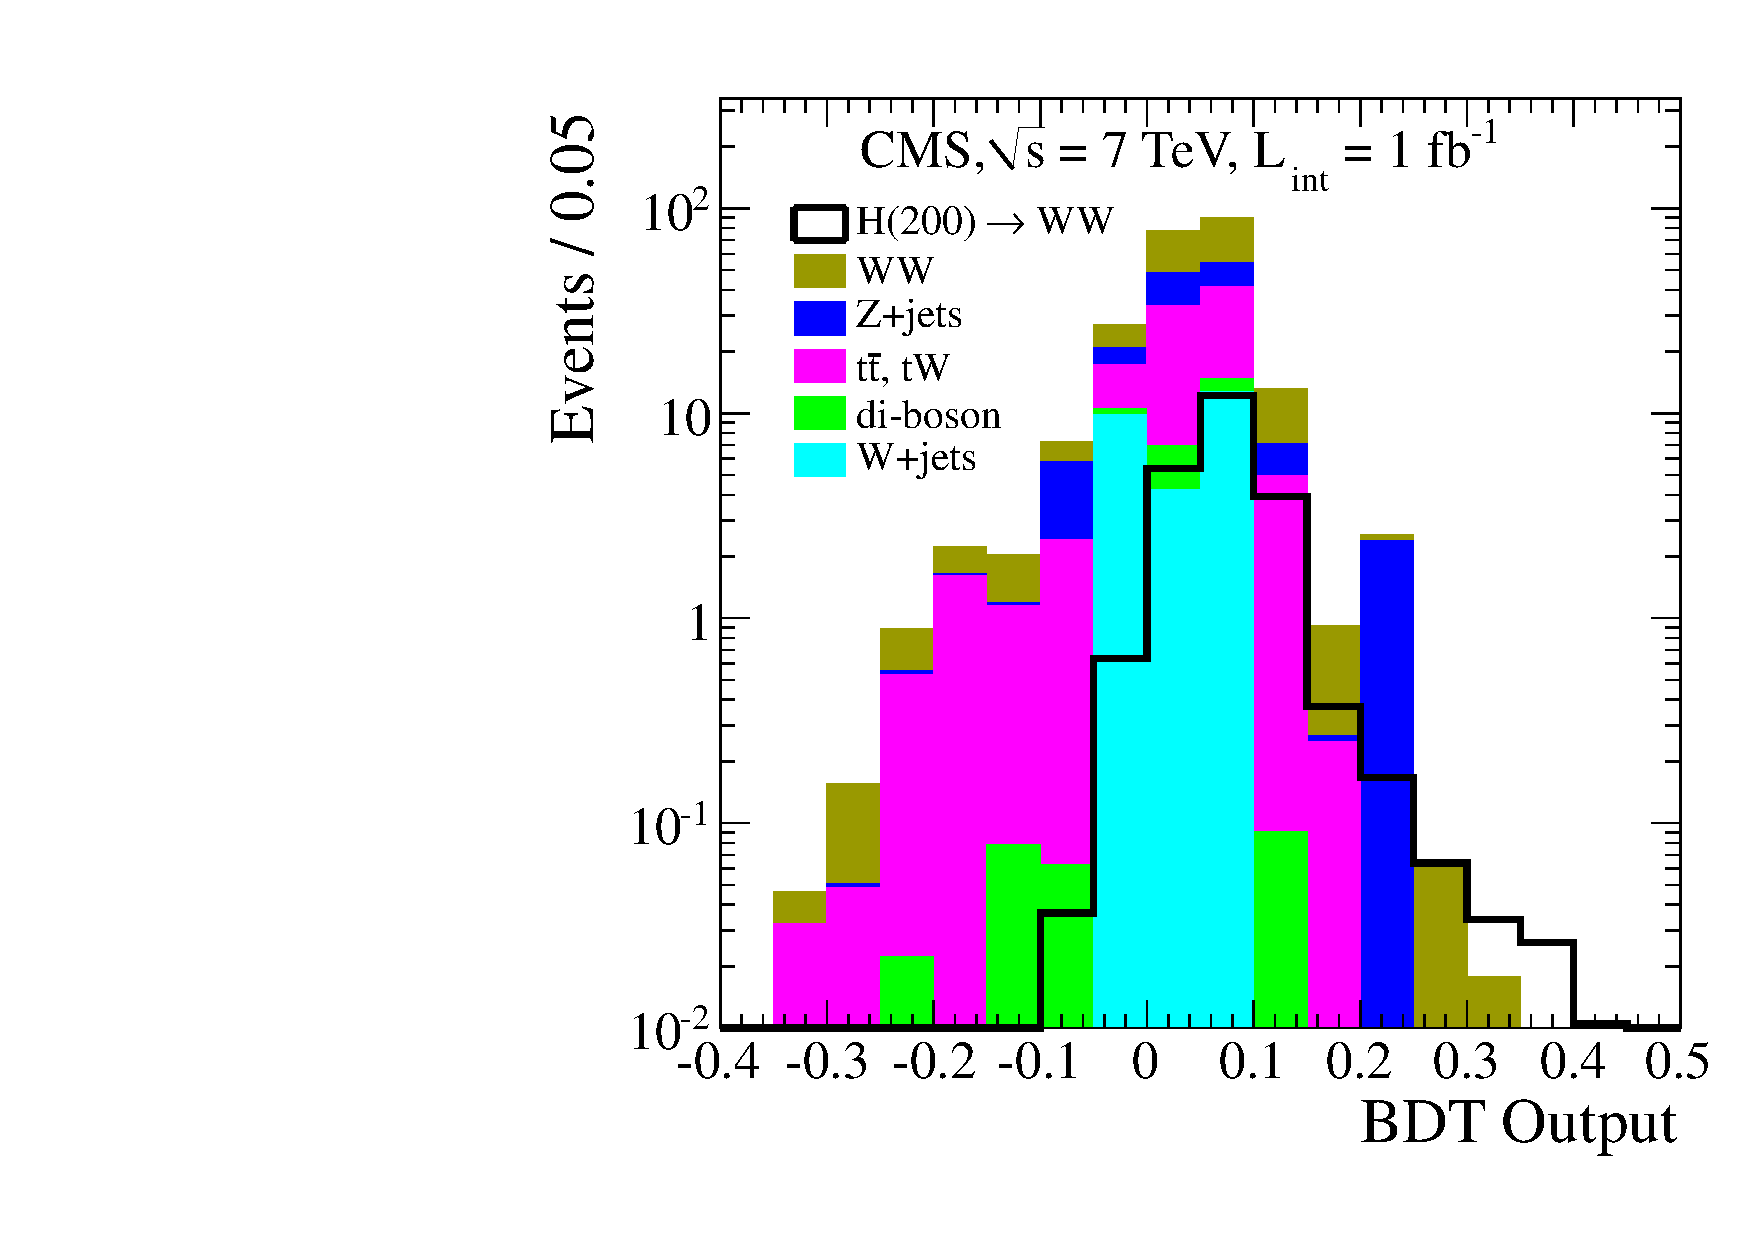
\includegraphics[width=0.49\textwidth,angle=0]{figures/histo_mva_200_1j.pdf}} 
       \caption{Classifier outputs for Higgs signal and background events 
for \mHi=200 $\GeVcc$ in the 0-jet bin (a) and 1-jet bin (b) after the $\WW$ selection. The number 
of events is different on each mass point due to the specific $\mll$ requirement.}
   \label{fig:histo_mva_200}
\end{center}
\end{figure}


\begin{table}[!ht]
  \begin{center}
 {\footnotesize
  \begin{tabular} {|c|c|c|c|c|c|c|c|}
\hline
  mass    & SM $H\to WW$ & all bkg. & $qq \to \WW$ & $gg \to \WW$ & all non-$\WW$ bkg. \\
  \hline
  \hline
120 &   2.18 $\pm$   0.06 &    5.55 $\pm$   0.22 &  4.71 $\pm$	0.20 & 0.27 $\pm$   0.02 & 0.57 $\pm$   0.10 \\
130 &   6.14 $\pm$   0.13 &   12.15 $\pm$   0.51 &  9.79 $\pm$	0.28 & 0.63 $\pm$   0.03 & 1.73 $\pm$   0.42 \\
140 &  10.82 $\pm$   0.21 &   17.68 $\pm$   1.06 & 13.53 $\pm$	0.34 & 0.95 $\pm$   0.04 & 3.20 $\pm$   1.00 \\
150 &  10.38 $\pm$   0.23 &    8.21 $\pm$   0.29 &  6.78 $\pm$	0.24 & 0.65 $\pm$   0.03 & 0.78 $\pm$   0.17 \\
160 &  11.05 $\pm$   0.24 &    2.31 $\pm$   0.14 &  1.79 $\pm$	0.12 & 0.32 $\pm$   0.02 & 0.19 $\pm$   0.07 \\
170 &  17.72 $\pm$   0.30 &    6.23 $\pm$   0.30 &  4.70 $\pm$	0.20 & 0.82 $\pm$   0.04 & 0.70 $\pm$   0.22 \\
180 &  10.64 $\pm$   0.20 &    6.26 $\pm$   0.46 &  4.15 $\pm$	0.18 & 0.80 $\pm$   0.04 & 1.31 $\pm$   0.42 \\
190 &   8.11 $\pm$   0.15 &    8.08 $\pm$   0.35 &  6.08 $\pm$	0.23 & 1.02 $\pm$   0.04 & 0.98 $\pm$   0.27 \\
200 &   8.05 $\pm$   0.14 &   11.23 $\pm$   0.42 &  8.32 $\pm$	0.26 & 1.34 $\pm$   0.05 & 1.57 $\pm$   0.32 \\
250 &   2.35 $\pm$   0.06 &    7.34 $\pm$   0.50 &  5.13 $\pm$	0.21 & 0.54 $\pm$   0.03 & 1.66 $\pm$   0.45 \\
300 &   2.20 $\pm$   0.05 &    8.05 $\pm$   0.47 &  5.68 $\pm$	0.22 & 0.47 $\pm$   0.03 & 1.89 $\pm$   0.42 \\
350 &   0.85 $\pm$   0.03 &    1.63 $\pm$   0.15 &  1.22 $\pm$	0.10 & 0.13 $\pm$   0.02 & 0.28 $\pm$   0.10 \\
400 &   3.32 $\pm$   0.05 &    9.19 $\pm$   0.56 &  6.38 $\pm$	0.23 & 0.56 $\pm$   0.03 & 2.25 $\pm$   0.51 \\
450 &   1.78 $\pm$   0.03 &    5.96 $\pm$   0.46 &  4.21 $\pm$	0.19 & 0.34 $\pm$   0.03 & 1.41 $\pm$   0.42 \\
500 &   1.07 $\pm$   0.02 &    4.22 $\pm$   0.37 &  2.81 $\pm$	0.15 & 0.38 $\pm$   0.03 & 1.03 $\pm$   0.34 \\
550 &   0.75 $\pm$   0.01 &    4.00 $\pm$   0.31 &  2.92 $\pm$	0.15 & 0.26 $\pm$   0.02 & 0.83 $\pm$   0.26 \\
600 &   0.26 $\pm$   0.01 &    0.86 $\pm$   0.13 &  0.62 $\pm$	0.07 & 0.10 $\pm$   0.01 & 0.14 $\pm$   0.10 \\
 \hline
  \end{tabular}
  }
 {\small
  \begin{tabular} {|c|c|c|c|c|}
\hline
  mass    & $\ttbar+tW$ & non-resonant $WZ$/$ZZ$ & $\dyll+WZ+ZZ$ & $\Wjets/\gamma$ \\
  \hline
  \hline
120 &  0.20 $\pm$   0.08 & 0.20 $\pm$   0.05 &  0.17 $\pm$   0.03 & 0.00 $\pm$ 0.00  \\
130 &  1.12 $\pm$   0.42 & 0.45 $\pm$   0.07 &  0.16 $\pm$   0.02 & 0.00 $\pm$ 0.00  \\
140 &  1.50 $\pm$   0.39 & 0.54 $\pm$   0.08 &  1.16 $\pm$   0.92 & 0.00 $\pm$ 0.00  \\
150 &  0.52 $\pm$   0.16 & 0.16 $\pm$   0.04 &  0.10 $\pm$   0.02 & 0.00 $\pm$ 0.00  \\
160 &  0.14 $\pm$   0.07 & 0.02 $\pm$   0.02 &  0.04 $\pm$   0.01 & 0.00 $\pm$ 0.00  \\
170 &  0.50 $\pm$   0.22 & 0.12 $\pm$   0.04 &  0.09 $\pm$   0.02 & 0.00 $\pm$ 0.00  \\
180 &  1.11 $\pm$   0.41 & 0.11 $\pm$   0.04 &  0.09 $\pm$   0.02 & 0.00 $\pm$ 0.00  \\
190 &  0.65 $\pm$   0.27 & 0.15 $\pm$   0.04 &  0.18 $\pm$   0.03 & 0.00 $\pm$ 0.00  \\
200 &  0.94 $\pm$   0.31 & 0.31 $\pm$   0.06 &  0.32 $\pm$   0.05 & 0.00 $\pm$ 0.00  \\
250 &  1.43 $\pm$   0.45 & 0.12 $\pm$   0.04 &  0.12 $\pm$   0.03 & 0.00 $\pm$ 0.00  \\
300 &  1.61 $\pm$   0.41 & 0.16 $\pm$   0.04 &  0.12 $\pm$   0.03 & 0.00 $\pm$ 0.00  \\
350 &  0.22 $\pm$   0.10 & 0.04 $\pm$   0.02 &  0.02 $\pm$   0.01 & 0.00 $\pm$ 0.00  \\
400 &  1.98 $\pm$   0.51 & 0.17 $\pm$   0.04 &  0.10 $\pm$   0.02 & 0.00 $\pm$ 0.00  \\
450 &  1.28 $\pm$   0.42 & 0.09 $\pm$   0.03 &  0.04 $\pm$   0.02 & 0.00 $\pm$ 0.00  \\
500 &  0.88 $\pm$   0.34 & 0.07 $\pm$   0.02 &  0.08 $\pm$   0.02 & 0.00 $\pm$ 0.00  \\
550 &  0.65 $\pm$   0.26 & 0.12 $\pm$   0.04 &  0.05 $\pm$   0.01 & 0.00 $\pm$ 0.00  \\
600 &  0.11 $\pm$   0.10 & 0.03 $\pm$   0.02 &  0.00 $\pm$   0.00 & 0.00 $\pm$ 0.00  \\
  \hline
  \hline

 \hline
  \end{tabular}
  }
  \caption{Expected number of signal and background processes for an 
  integrated luminosity of 1 $\ifb$, after applying the full multivariate analysis 
  selection in the 0-jet bin case. Monte Carlo statistical uncertainties are included.}
   \label{tab:mvasel0j}
  \end{center}
\end{table}

\begin{table}[!ht]
  \begin{center}
 {\footnotesize
  \begin{tabular} {|c|c|c|c|c|c|c|c|}
\hline
  mass    & SM $H\to WW$ & all bkg. & $qq \to \WW$ & $gg \to \WW$ & all non-$\WW$ bkg. \\
  \hline
  \hline
120 &  1.46 $\pm$   0.04 &    7.11 $\pm$   1.43 &  3.17 $\pm$   0.16 &  0.13 $\pm$   0.02 &   3.81 $\pm$   1.42 \\
130 &  2.42 $\pm$   0.07 &    6.28 $\pm$   1.70 &  2.81 $\pm$   0.15 &  0.14 $\pm$   0.02 &   3.34 $\pm$   1.69 \\
140 &  9.85 $\pm$   0.17 &   22.46 $\pm$   2.39 &  9.98 $\pm$   0.29 &  0.58 $\pm$   0.03 &  11.90 $\pm$   2.38 \\
150 &  8.06 $\pm$   0.16 &   11.60 $\pm$   2.00 &  5.07 $\pm$   0.20 &  0.35 $\pm$   0.03 &   6.18 $\pm$   1.99 \\
160 & 13.98 $\pm$   0.22 &   11.60 $\pm$   2.41 &  4.25 $\pm$   0.19 &  0.37 $\pm$   0.03 &   6.98 $\pm$   2.40 \\
170 & 13.84 $\pm$   0.21 &   13.14 $\pm$   2.36 &  5.71 $\pm$   0.22 &  0.54 $\pm$   0.03 &   6.89 $\pm$   2.35 \\
180 &  9.58 $\pm$   0.16 &   14.15 $\pm$   2.37 &  6.00 $\pm$   0.22 &  0.59 $\pm$   0.03 &   7.56 $\pm$   2.36 \\
190 &  5.07 $\pm$   0.10 &   12.12 $\pm$   1.93 &  5.12 $\pm$   0.20 &  0.44 $\pm$   0.03 &   6.55 $\pm$   1.92 \\
200 &  8.99 $\pm$   0.12 &   36.07 $\pm$   3.03 & 15.64 $\pm$   0.36 &  1.20 $\pm$   0.05 &  19.23 $\pm$   3.01 \\
250 &  3.17 $\pm$   0.06 &   25.48 $\pm$   3.19 &  8.79 $\pm$   0.27 &  0.40 $\pm$   0.03 &  16.29 $\pm$   3.18 \\
300 &  1.56 $\pm$   0.03 &   10.48 $\pm$   1.81 &  3.88 $\pm$   0.18 &  0.14 $\pm$   0.02 &   6.46 $\pm$   1.80 \\
350 &  2.24 $\pm$   0.04 &   12.40 $\pm$   2.11 &  4.32 $\pm$   0.19 &  0.24 $\pm$   0.02 &   7.84 $\pm$   2.10 \\
400 &  2.16 $\pm$   0.03 &   10.47 $\pm$   1.60 &  3.64 $\pm$   0.17 &  0.23 $\pm$   0.02 &   6.60 $\pm$   1.59 \\
450 &  0.44 $\pm$   0.01 &    1.53 $\pm$   0.29 &  0.93 $\pm$   0.09 &  0.02 $\pm$   0.01 &   0.58 $\pm$   0.28 \\
500 &  0.34 $\pm$   0.01 &    1.37 $\pm$   0.18 &  0.93 $\pm$   0.09 &  0.03 $\pm$   0.01 &   0.42 $\pm$   0.16 \\
550 &  0.50 $\pm$   0.01 &    2.77 $\pm$   0.35 &  1.59 $\pm$   0.11 &  0.09 $\pm$   0.01 &   1.09 $\pm$   0.33 \\
600 &  0.19 $\pm$   0.00 &    0.92 $\pm$   0.10 &  0.77 $\pm$   0.08 &  0.04 $\pm$   0.01 &   0.12 $\pm$   0.05 \\
 \hline
  \end{tabular}
  }
 {\small
  \begin{tabular} {|c|c|c|c|c|}
\hline
  mass    & $\ttbar+tW$ & non-resonant $WZ$/$ZZ$ & $\dyll+WZ+ZZ$ & $\Wjets/\gamma$ \\
  \hline
  \hline
120 &   1.16 $\pm$   0.35 & 0.20 $\pm$   0.05 &  2.45 $\pm$   1.38 & 0.00 $\pm$   0.00  \\
130 &   0.78 $\pm$   0.25 & 0.17 $\pm$   0.04 &  2.39 $\pm$   1.67 & 0.00 $\pm$   0.00  \\
140 &   6.53 $\pm$   0.97 & 0.53 $\pm$   0.08 &  4.84 $\pm$   2.17 & 0.00 $\pm$   0.00  \\
150 &   2.93 $\pm$   0.64 & 0.18 $\pm$   0.04 &  3.07 $\pm$   1.88 & 0.00 $\pm$   0.00  \\
160 &   1.74 $\pm$   0.40 & 0.10 $\pm$   0.03 &  5.14 $\pm$   2.36 & 0.00 $\pm$   0.00  \\
170 &   2.18 $\pm$   0.52 & 0.18 $\pm$   0.05 &  4.54 $\pm$   2.29 & 0.00 $\pm$   0.00  \\
180 &   2.94 $\pm$   0.58 & 0.10 $\pm$   0.03 &  4.52 $\pm$   2.28 & 0.00 $\pm$   0.00  \\
190 &   3.32 $\pm$   0.70 & 0.13 $\pm$   0.04 &  3.11 $\pm$   1.79 & 0.00 $\pm$   0.00  \\
200 &  12.05 $\pm$   1.33 & 0.39 $\pm$   0.06 &  6.78 $\pm$   2.70 & 0.00 $\pm$   0.00  \\
250 &   7.71 $\pm$   1.12 & 0.18 $\pm$   0.04 &  8.39 $\pm$   2.97 & 0.00 $\pm$   0.00  \\
300 &   3.48 $\pm$   0.81 & 0.03 $\pm$   0.02 &  2.95 $\pm$   1.61 & 0.00 $\pm$   0.00  \\
350 &   3.71 $\pm$   0.73 & 0.06 $\pm$   0.03 &  4.07 $\pm$   1.97 & 0.00 $\pm$   0.00  \\
400 &   4.67 $\pm$   0.88 & 0.10 $\pm$   0.04 &  1.83 $\pm$   1.33 & 0.00 $\pm$   0.00  \\
450 &   0.57 $\pm$   0.28 & 0.00 $\pm$   0.00 &  0.01 $\pm$   0.00 & 0.00 $\pm$   0.00  \\
500 &   0.40 $\pm$   0.16 & 0.01 $\pm$   0.01 &  0.01 $\pm$   0.00 & 0.00 $\pm$   0.00  \\
550 &   1.04 $\pm$   0.33 & 0.03 $\pm$   0.02 &  0.02 $\pm$   0.01 & 0.00 $\pm$   0.00  \\
600 &   0.10 $\pm$   0.05 & 0.01 $\pm$   0.01 &  0.01 $\pm$   0.00 & 0.00 $\pm$   0.00  \\
  \hline
  \hline

 \hline
  \end{tabular}
  }
  \caption{Expected number of signal and background processes for an 
  integrated luminosity of 1 $\ifb$, after applying the full multivariate analysis 
  selection in the 1-jet bin case. Monte Carlo statistical uncertainties are included.}
   \label{tab:mvasel1j}
  \end{center}
\end{table}


\clearpage
\section{Background Estimation}
   \label{sec:backgrounds}
   We use a combination of data-driven methods and detailed Monte Carlo
simulation studies to estimate background contributions.  From data we
can estimate the following backgrounds: $\Wjets$, $\dyll$, $\WZ$ and
$\ZZ$ (for events where both leptons come from a $\dyll$), top
background and \WW{}. The background from the remaining processes 
are taken from simulation.

Background composition and yields depend on the final state and on
the Higgs boson mass hypothesis under study. In the 0-Jet final state, 
the non-resonant \WW{} background dominates, while \wjets\ background contribution 
becomes sizable in the low Higgs mass hypotheses (see Table~\ref{tab:wwselection0}). 
In the 1-Jet and 2-Jet final states, the largest background contribution comes from 
top decays, while the non-resonant \ww\ background contribution is the second largest. 

For the backgrounds that can be estimated from data, 
we perform a data-driven background estimate in the signal region 
if the expected background contribution is sizable. 
If the expected contribution in the signal region is limited by statistics, 
we first estimate the background contribution with the $WW$ preselection from data 
and then extrapolate this estimation to the signal region using MC. The particular
choice of which backgrounds are estimated in the first or second way depends on the
integrated luminosity of the data sample that we analyze. 

%For the backgrounds that are expected to have a sizable number of events after
%final Higgs cuts we perform a data driven background estimation for
%the final selection. If the expected number of background events is
%small (just a few event), we estimate the background at the \WW\
%selection level and scale it down for a final selection using the
%Monte Carlo predicted scale factors.

   \label{sec:bkg_intro}
% \subsection{$\ZZ$ and resonant~$\WZ$ Background}
%    \label{sec:bkg_ww}
%    The basic idea for the estimation of the nonresonant $WW$ contribution in the $\hww$ signal region is 
to infer it from data using the dilepton mass distribution:
the dilepton mass defines a control region where we can measure the $WW$ normalization, and then scale
the contribution to the signal region.

It turns out that this approach can be applied for $m_H \leq 200~\GeVcc$ only.
In fact, MC studies show that the di-lepton mass distribution in Higgs samples has a cut-off value at $m_H-50~\GeVcc$;
thus, for large $m_H$ it is possible to define an Higgs-depleted region only in a mass range populated by too 
few $WW$ events. 

Therefore, for $m_H > 200~\GeVcc$ the $WW$ contribution is estimated from MC.

\subsubsection{Estimation procedure in low mass range}

For low Higgs boson mass values ($m_{\rm{H}} \leq 200~\GeVcc$) events with $m_{\ell\ell} > 100~\GeVcc$ are used
to define a control region where the Higgs contribution is $<3\%$.

The procedure is as follows:
\begin{itemize}
\item the yield in the control region is measured after the lepton and jet selections 
(i.e. full selection except $m_{l,l}$, $m_T$ and $\Delta\phi_{ll}$ cuts) so that most of the systematics uncertainties 
cancel out (e.g. jet veto, lepton and trigger efficiencies); 
\item the contamination from other backgrounds (mainly $t\bar t$ and $W$+jets, for a total of $\sim$ 20\%) 
is subtracted using the corresponding data-driven techniques;
\item the obtained yield is scaled to the signal region using the control-to-signal region ratio from MC;
\item finally, the MC efficiency for $m_T$ and $\Delta\phi_{ll}$ cut is accounted to obtain the $WW$ contribution in the 
signal region after all cuts.
\end{itemize}

In order to consider this procedure as reliable we verify that 
the control-to-signal region ratio is stable using different generators and 
we check that the efficiency of the $m_T$ and $\Delta\phi_{ll}$ cuts in the control region in data and MC is consistent.

%Systematics are evaluated repeating the procedure varying the usual suspects.

%
%\subsection{Estimation in high mass range}
%We take it from MC.



%The nonresonant $qq \to \WW$ contribution in the $\hww$ signal region is 
%estimated from data using the dilepton mass distribution. For a given Higgs 
%boson mass, the region with a small contribution from Higgs boson decays is 
%selected and simulation is used to extrapolate this background into the signal 
%region. For low Higgs boson mass values ($m_{\rm{H}} < 200~\GeVcc$) events 
%with $m_{\ell\ell} > 100~\GeVcc$ are used, while for $m_{\rm{H}} > 200~\GeVcc$ 
%events with $m_{\ell\ell} < 100~\GeVcc$ are used. The statistical uncertainty 
%on the estimate of the nonresonant $\WW$ background with the current data 
%sample is approximately 50\%. For the 1- and 2- jet bin cases we use the results
%from the 0-jet bin, and then extrapolate to each jet bin.
%
%The $gg \to \WW$ background contribution has to be taken from simulated events 
%since we do not have enough sensitivity in the data to measure it. We assign a 
%50\% uncertainty to the overall normalization~\cite{ggWWError}. This is 
%obtained by studying the change in the cross-section when varying the parton 
%distribution functions (PDFs), QCD renormalization and scales.

  \subsection{Drell-Yan Background}
    \label{sec:bkg_dy}
    Since the production cross-section for Drell-Yan is several orders of magnitude 
higher than the $H \to ZZ$ signal, the Drell-Yan background poses a significant 
challenge. To the leading order, the Drell-Yan process does not contain \met\,  
and therefore its contribution is signficantly reduced by a tight \met selection. 
The residual Drell-Yan contribution in the signal region 
is mainly due to events with fake \met either due to energy mismeasurement of  
the hadronic recoil or momentum mismeasurement of the selected leptons. 
The contribution of events with fake \met due to the lepton momentum mismeasurement 
is expected to be small since we select events within a fairly tight (within $15$ GeV) window 
around the $Z$ boson pole mass. The background due to mismeasurement of the hadronic
recoil is the main source of Drell-Yan events contributing to the selected signal region.

The estimation of residual Drell-Yan background in the signal region depends highly 
our understanding of the \met tails which is sensitive to many factors such as 
the jet energy corrections, the number of pileup interactions, and energy from out of time
contributions. These effects are difficult to model precisely in the simulation.
Therfore we employ a data-driven method to estimate the \met distribution for the 
Drell-Yan background. For events without natural \met\, under the assumption that 
the fake \met is only resulting from mismeasurement of the hadronic recoil, we can use
$\gamma$+jets events as a control sample to predict the \met distribution in $Z$+jets
background events. If parameterized correctly in an observable that is highly correlated 
with the source of fake \met, one expects $\gamma$+jets events to provide an accurate
model of the \met distribution for $Z$+jets events, provided that the photon
is well measured and does not contribute to the \met.

\subsubsection{Photon Selection and Reweighting Procedure}
The photon data sample is selected by requiring one and only one photon passing reaonsably tight
identification and isolation requirements, summarized in Table \ref{tab:PhotonSelection} below 
\cite{MITHggNote}. 
An electron veto is imposed on the photon, requiring that no GSF electron which does not match to 
one leg of a well reconstructed convert is sharing the same supercluster as the photon
candidate. This is intended to reduce contributions from W bosons decaying to electrons, misidentified
as photons. To reduce contamination from $W$+$\gamma$ events, we veto any events with one or 
more well identified leptons.


\begin{table}[!ht]
\begin{center}
\begin{tabular}{|c|c|} 
\hline
Cut           & Requirement                                                                           \\
\hline
$\eta$        & $|\eta| < 1.4442$                                                                     \\ 
\hline
H/E           & H/E $< 0.05$                                                                          \\
\hline
Electron Veto & Photon is rejected if it shares the supercluster with an electron that does not       \\
              & match to one leg of a conversion with $\mathrm{L}_{\mathrm{xy}} < 2.0$, fit           \\
              & probability  $> 10^{-6}$, and no hits behind the fitted vertex                        \\
\hline
\hline
\multicolumn{2}{|c|}{Conversion ID (if matched to a conversion with $\mathrm{L}_{\mathrm{xy}} < 2.0$,}\\
\multicolumn{2}{|c|}{fit probability $> 10^{-6}$, and at most one hit before the fitted vertex on }   \\
\multicolumn{2}{|c|}{either of the tracks forming the conversion) }                                   \\
\hline
E/P            & E/P $< 2.0 $                                                                         \\
%$\Delta\eta$  & $|\Delta\eta| < 0.01 for Endcap only$ \\
%$\Delta\phi$  & $|\Delta\phi| < 0.01 for Endcap only$ \\
\hline
\hline
\multicolumn{2}{|c|}{Isolation}                                                                       \\
\hline
EcalIso       & EcalIso $ - \rho\times \mathrm{A}_{\mathrm{eff Ecal}}$ $<  2.0 + 0.006\times p_{T}$   \\
HcalIso       & HcalIso $ - \rho\times \mathrm{A}_{\mathrm{eff Hcal}}$ $<  2.0 + 0.0025\times p_{T}$  \\
TrkIso        & TrkIso $ - \rho\times \mathrm{A}_{\mathrm{eff Trk}}$ $<  1.5 + 0.001\times p_{T}$     \\
\hline

%\hline
%SpikeKilling & \\
%\hline
%$E_{\mathrm{Max}} / E_{9}$ & $E_{\mathrm{Max}} / E_{9} > 0.95$       \\
%$\sigma_{i\eta i\eta}$     & $\sigma_{i\eta i\eta} > 0.001$          \\
%$\sigma_{i\phi i\phi}$     & $\sigma_{i\phi i\phi} > 0.001$          \\
%\hline

\hline
\end{tabular}
\caption{MC yield prediction for $H\rightarrow WW$ sample ($m_H=130$ GeV) ($\mu$-e and e-e final states). 
The electron selection is the same as in 2010 analysis and the results is scaled to 1/fb.
\label{tab:PhotonSelection}}
\end{center}
\end{table}


Since the fake \met is due to mismeasurement of the hadronic recoil, we parameterize the 
modelling of the \met distribution in the $p_{T}$ of the photon / dilepton system and 
the number of counted jets. Both variables are highly correlated with the behavior 
of the hadronic recoil. Reweighting factors are computed in bins of the number of counted jets
and the dilepton $p_{T}$ by dividing the corresponding two dimensional distributions
in the $\gamma$+jets data sample and the dilepton data sample:

\begin{eqnarray}
  w(p_{T},\mathrm{njet}) = \frac{\mathrm{N}_{\gamma+\mathrm{jets}}(p_{T},\mathrm{njet})}{\mathrm{N}_{\mathrm{Z+jets}}(p_{T},\mathrm{njet})}.
\end{eqnarray}

In order for these reweighting factors to be insensitive to the presence of signal or backgrounds with 
real \met, we build these weight factors on a $\gamma$+jets and $Z$+jets sample imposing an anti-selection
on the \met : $\met < 30$ GeV. For the $Z$+jets sample, the full $H \to ZZ$ preselection is imposed, 
including the top veto and the third lepton veto.

Finally, to model the \met distribution for the final selection we select $\gamma$+jets events
as above, imposing the preselection requirement that the photon $p_{T}$ is greater than $40$GeV,
and associate the corresponding weight factor $w(p_{T},\mathrm{njet})$ to each such event. To build
the track \met in the $\gamma$+jets events, we must consistently account for the momentum of
the photon since we intend it to model the dilepton system which would be included in the 
track \met in $Z$+jets events. To mitigate cases of inconsistencies between the particle flow 
photon reconstruction and the standard photon reconstruction, particularly for converted photons,
we do not include any charged particle flow candidates inside the ($\Delta$R $<0.4$) isolation cone 
of the photon in the track \met sum.
To model the transverse mass distribution, we draw a random number from a pre-determined dilepton
mass distribution and build the $m_{T}$ observable as in Eqn \ref{}. The dilepton mass distribution
is constructed from data imposing all preselection cuts except the \met requirement.

\subsubsection{Monte Carlo Closure Test}

In order to verify that the procedure models the $Z$+jet background well, we test it
in $\gamma$+jets and $Z$+jets Monte Carlo simulation. The reweighting factors are 
built from the simulation sample according to the procedure described above and then 
applied on the $\gamma$+jets Monte Carlo sample. 

%The photon and $Z$ 
%$p_{T}$ distributions are shown in Fig \ref{fig:PhotonJetsClosureTest_Pt} to demonstrate that 
%the reweighting is carried out consistently.

%% \begin{figure}[!htbp]
%% \begin{center}
%% \subfigure[0-Jet]{\includegraphics[width=0.45\textwidth]{figures/PhotonJetsClosureTest_0Jet_Pt.pdf}}
%% \subfigure[1-Jet]{\includegraphics[width=0.45\textwidth]{figures/PhotonJetsClosureTest_1Jet_Pt.pdf}}
%% \subfigure[2-Jet]{\includegraphics[width=0.45\textwidth]{figures/PhotonJetsClosureTest_2Jet_Pt.pdf}}
%% \caption{Comparison of the dilepton $p_{T}$ and the photon $p_{T}$ before and after reweighting.}
%% \label{fig:PhotonJetsClosureTest_Pt}
%% \end{center}
%% \end{figure}


In Fig \ref{fig:PhotonJetsClosureTest_TrackMET} we show the particle flow \met distribution 
from the $\gamma$+jet sample after reweighting compared to the \met distribution from the 
$Z$+jet sample, separately in the 0-jet, 1-jet, and 2-jet bins. We observe agreement between 
the $\gamma$+jet generated prediction and the $Z$+jet simulation particle flow \met distribution. 
In Fig \ref{fig:PhotonJetsClosureTest_TrackMET} we show the analogous comparison for track \met, where 
is agreement slightly worse than for particle flow \met. Finally, in 
Fig \ref{fig:PhotonJetsClosureTest_TrackMET}, we show the comparison for the minimum of the 
track \met and the particle flow \met, which shows better agreement than the track \met alone. 

\begin{figure}[!htbp]
\begin{center}
\subfigure[0-Jet]{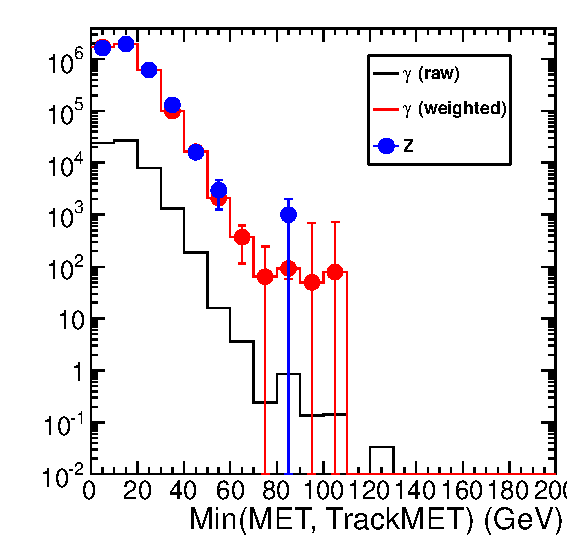
\includegraphics[width=0.45\textwidth]{figures/PhotonJetsClosureTest_0Jet_PFMET.pdf}}
\subfigure[1-Jet]{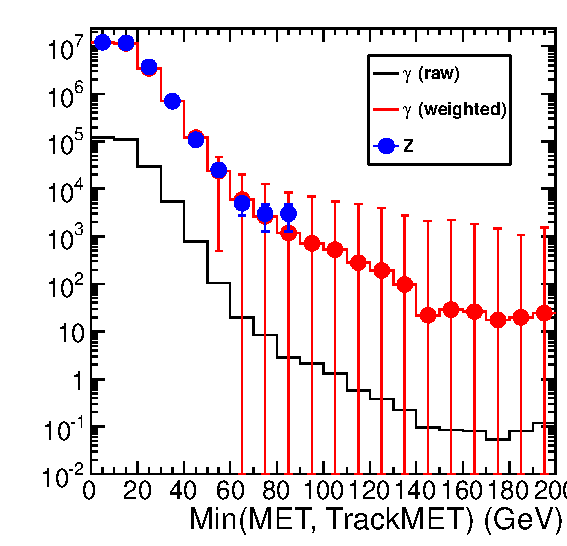
\includegraphics[width=0.45\textwidth]{figures/PhotonJetsClosureTest_1Jet_PFMET.pdf}}
\subfigure[2-Jet]{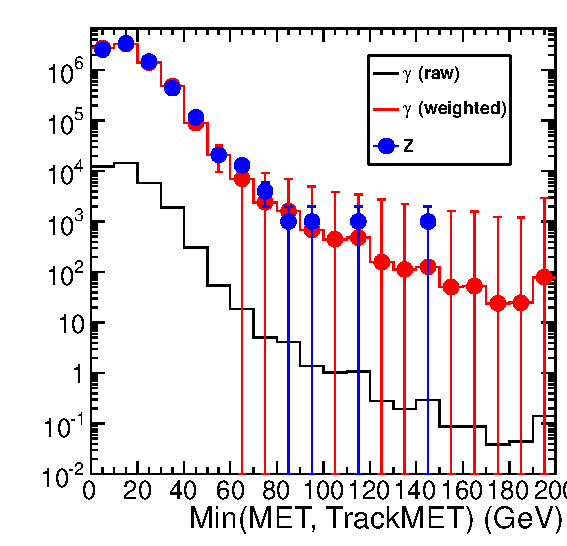
\includegraphics[width=0.45\textwidth]{figures/PhotonJetsClosureTest_2Jet_PFMET.pdf}}
\caption{Comparison of the particle flow \met prediction from the reweighted $\gamma$+jets sample
and the simulation prediction from the $Z$+jets sample.}
\label{fig:PhotonJetsClosureTest_TrackMET}
\end{center}
\end{figure}

\begin{figure}[!htbp]
\begin{center}
\subfigure[0-Jet]{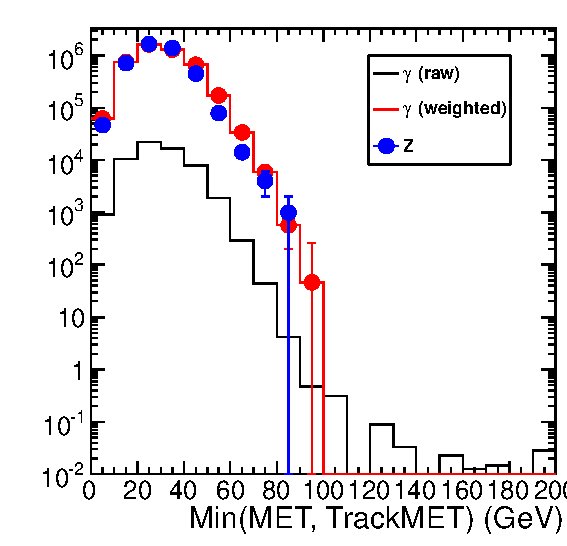
\includegraphics[width=0.45\textwidth]{figures/PhotonJetsClosureTest_0Jet_TrackMET.pdf}}
\subfigure[1-Jet]{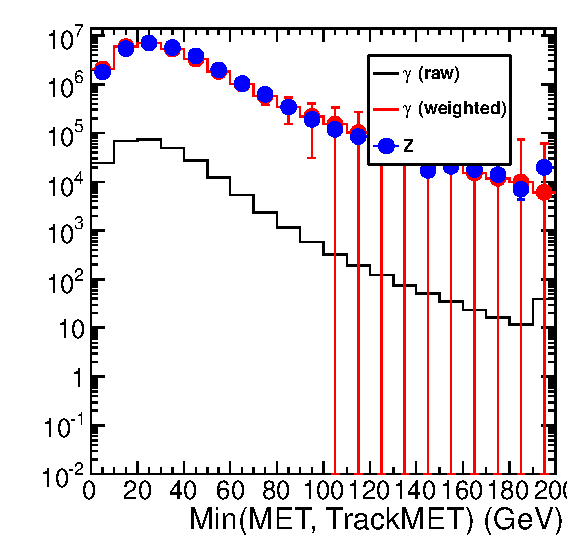
\includegraphics[width=0.45\textwidth]{figures/PhotonJetsClosureTest_1Jet_TrackMET.pdf}}
\subfigure[2-Jet]{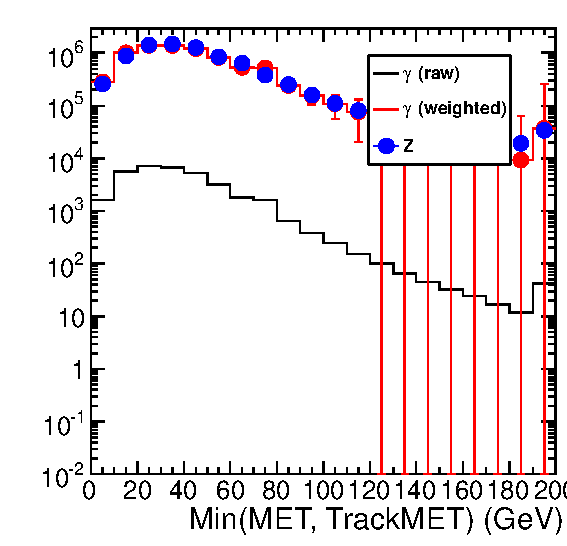
\includegraphics[width=0.45\textwidth]{figures/PhotonJetsClosureTest_2Jet_TrackMET.pdf}}
\caption{Comparison of the particle flow track \met prediction from the reweighted $\gamma$+jets sample
and the simulation prediction from the $Z$+jets sample.}
\label{fig:PhotonJetsClosureTest_TrackMET}
\end{center}
\end{figure}

\begin{figure}[!htbp]
\begin{center}
\subfigure[0-Jet]{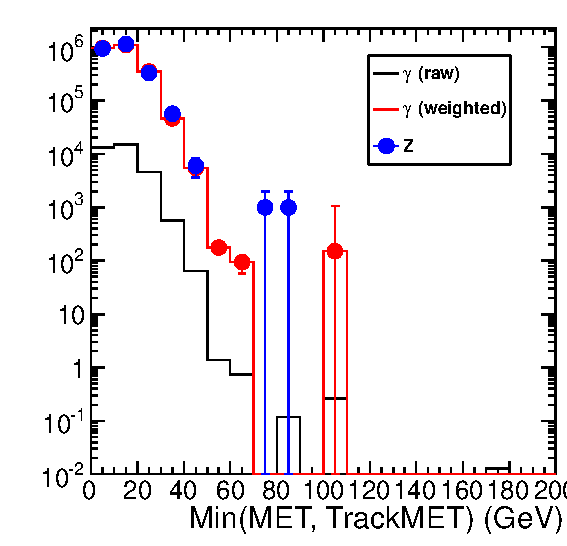
\includegraphics[width=0.45\textwidth]{figures/PhotonJetsClosureTest_0Jet_MinMET.pdf}}
\subfigure[1-Jet]{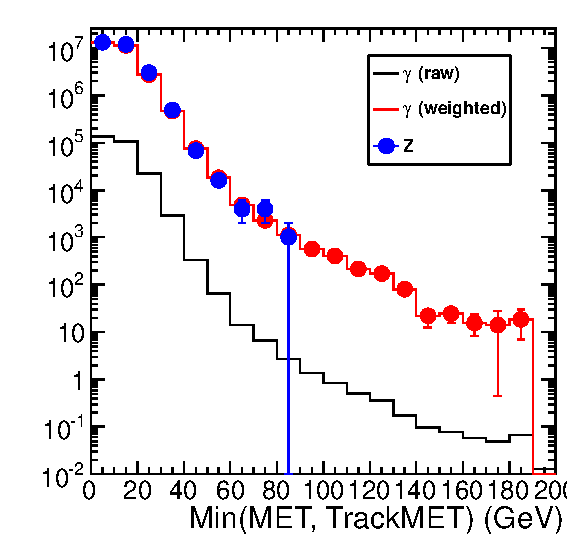
\includegraphics[width=0.45\textwidth]{figures/PhotonJetsClosureTest_1Jet_MinMET.pdf}}
\subfigure[2-Jet]{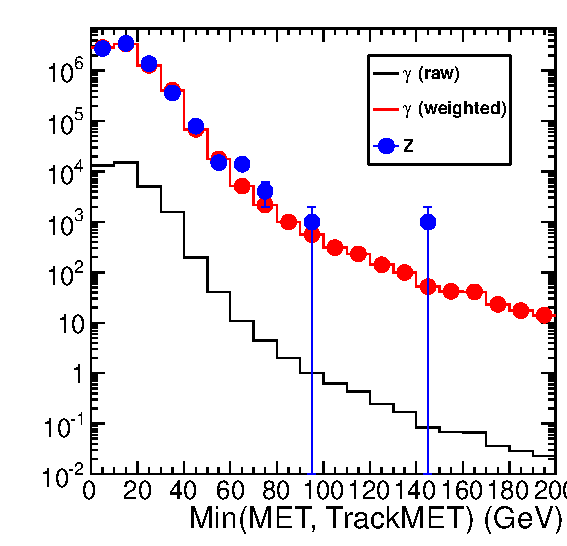
\includegraphics[width=0.45\textwidth]{figures/PhotonJetsClosureTest_2Jet_MinMET.pdf}}
\caption{Comparison of the minimum of particle flow \met and particle flow track \met prediction from
the reweighted $\gamma$+jets sample and the simulation prediction from the $Z$+jets sample.}
\label{fig:PhotonJetsClosureTest_TrackMET}
\end{center}
\end{figure}

\begin{figure}[!htbp]
\begin{center}
\subfigure[0-Jet]{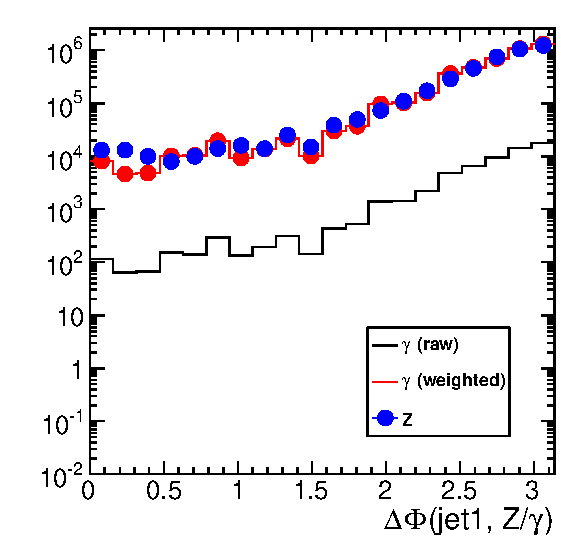
\includegraphics[width=0.45\textwidth]{figures/PhotonJetsClosureTest_0Jet_Dphi.pdf}}
\subfigure[1-Jet]{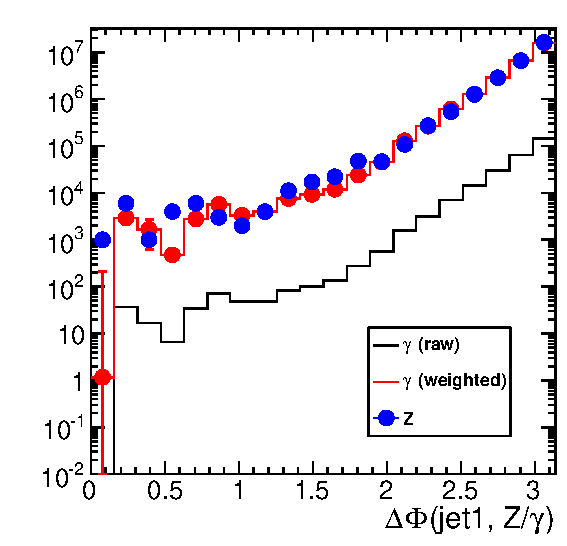
\includegraphics[width=0.45\textwidth]{figures/PhotonJetsClosureTest_1Jet_Dphi.pdf}}
\subfigure[2-Jet]{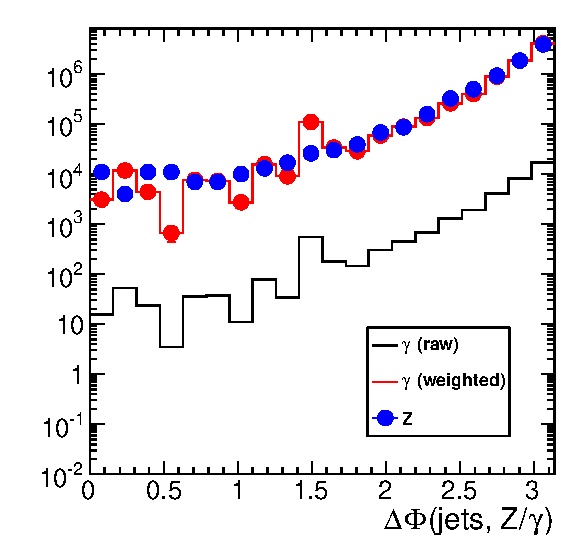
\includegraphics[width=0.45\textwidth]{figures/PhotonJetsClosureTest_2Jet_Dphi.pdf}}
\caption{Comparison of the $\Delta\phi$ between the dilepton system and the leading jet 
(with $p_{T} > 15$ GeV) in the event between the reweighted $\gamma$+jets sample and the 
simulation prediction from the $Z$+jets sample.}
\label{fig:PhotonJetsClosureTest_DPhi}
\end{center}
\end{figure}


Finally, we show the comparison between the predicted transverse mass distribution and the simulation
distribution with no cut on minimum \met in Fig \ref{fig:PhotonJetsClosureTest_MtHZZ_NoMetCut} and 
with a minimum \met cut of greater than $40$GeV in Fig \ref{fig:PhotonJetsClosureTest_MtHZZ_MetPresel}. 
The predicted shape and the simulation shape are again in reasonable agreement. 

\begin{figure}[!htbp]
\begin{center}
\subfigure[0-Jet]{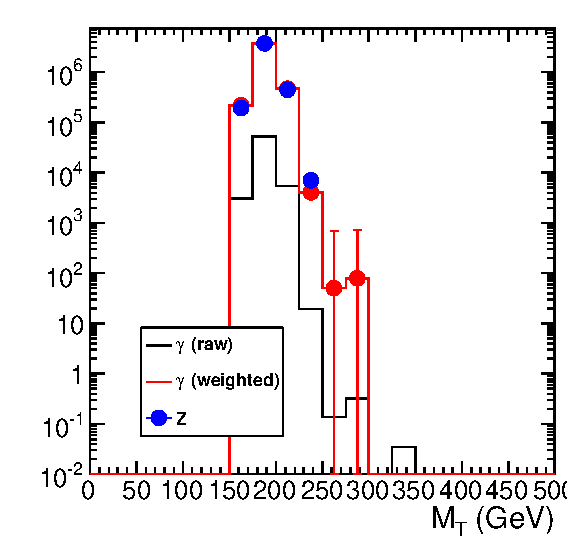
\includegraphics[width=0.45\textwidth]{figures/PhotonJetsClosureTest_0Jet_MtHZZ_NoMetCut.pdf}}
\subfigure[1-Jet]{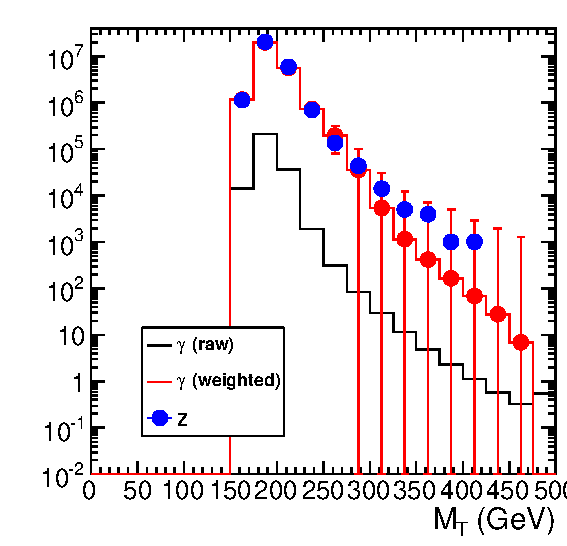
\includegraphics[width=0.45\textwidth]{figures/PhotonJetsClosureTest_1Jet_MtHZZ_NoMetCut.pdf}}
\subfigure[2-Jet]{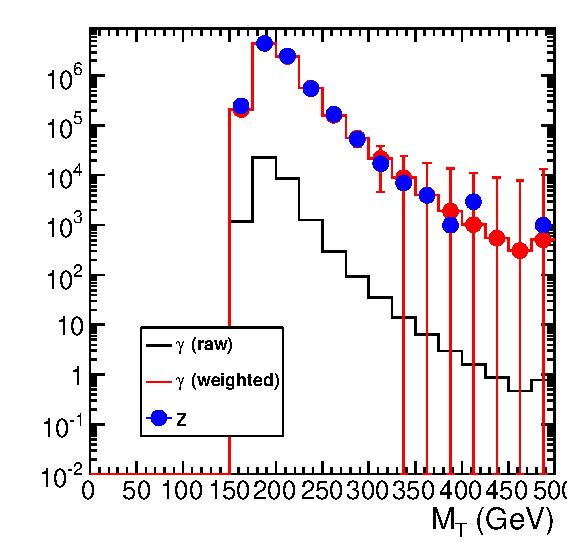
\includegraphics[width=0.45\textwidth]{figures/PhotonJetsClosureTest_2Jet_MtHZZ_NoMetCut.pdf}}
\caption{Comparison of the transverse mass prediction from the reweighted $\gamma$+jets sample 
and the simulation prediction from the $Z$+jets sample, where no \met cut has been applied.}
\label{fig:PhotonJetsClosureTest_MtHZZ_NoMetCut}
\end{center}
\end{figure}

\begin{figure}[!htbp]
\begin{center}
\subfigure[0-Jet]{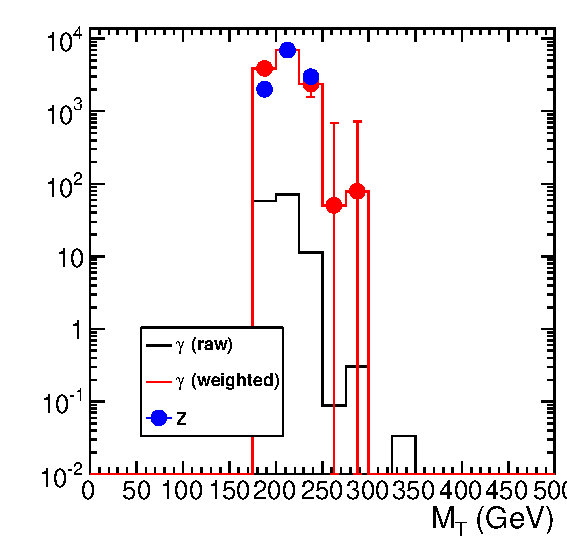
\includegraphics[width=0.45\textwidth]{figures/PhotonJetsClosureTest_0Jet_MtHZZ_MetPresel.pdf}}
\subfigure[1-Jet]{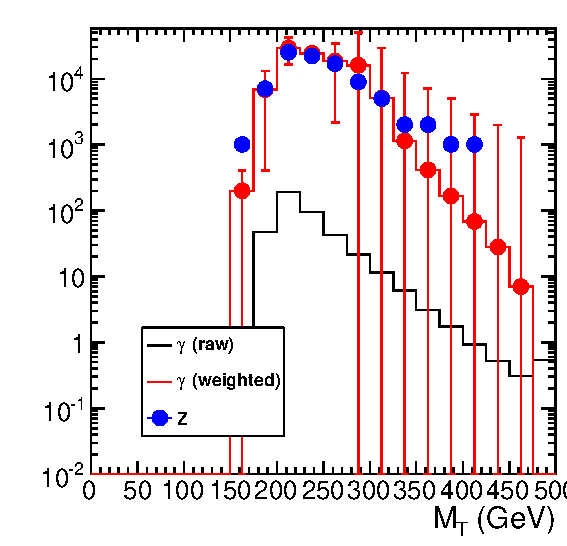
\includegraphics[width=0.45\textwidth]{figures/PhotonJetsClosureTest_1Jet_MtHZZ_MetPresel.pdf}}
\subfigure[2-Jet]{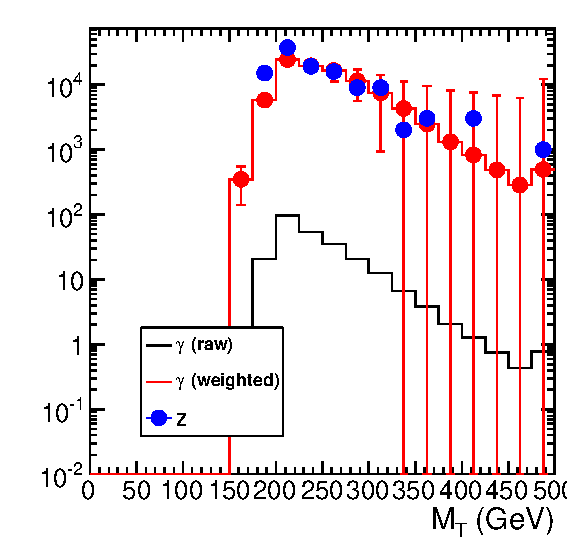
\includegraphics[width=0.45\textwidth]{figures/PhotonJetsClosureTest_2Jet_MtHZZ_MetPresel.pdf}}
\caption{Comparison of the transverse mass prediction from the reweighted $\gamma$+jets sample 
and the simulation prediction from the $Z$+jets sample, where the minimum \met is required to be larger than 
$40$ GeV. }
\label{fig:PhotonJetsClosureTest_MtHZZ_MetPresel}
\end{center}
\end{figure}


%We work on this section more later
%\subsubsection{Systematic Uncertainties}

Based on the degree of overall disagreement in the full range of the minimum \met we assign 
systematic uncertainties of $30\%$ in all the jet bins.


\subsubsection{Data Estimate}

The predictions for the minimum \met is compared with the results obtained in the first $187$\ipb 
of Run2011 data in Fig \ref{}, separately for the 0-jet, 1-jet, and 2-jet bins. Including all of the
backgrounds with real \met, we obtain reasonable agreement with data. 

Based on the $\gamma$+jet sample prediction, we obtain the background predictions for the
preselection and all the mass dependent cut-based analyses summarized in Table \ref{tab:DYBkgPrediction}.

\begin{table}[!htbp]
\begin{center}
\begin{tabular}{|l|c|c|c|c|}
\hline
Higgs Mass      &  0-jet bin             & 1-jet bin             & 2-jet bin             & Total                \\
\hline
ZZ Preselection &  $0.01 \pm 0.00$(stat) & $0.08 \pm 0.02$(stat) & $0.22 \pm 0.07$(stat) $ 0.31 \pm 0.11$(stat) \\
\hline
250             &  $0.01 \pm 0.00$(stat) & $0.08 \pm 0.02$(stat) & $0.22 \pm 0.07$(stat) $ 0.31 \pm 0.11$(stat) \\
300             &  $0.01 \pm 0.00$(stat) & $0.08 \pm 0.02$(stat) & $0.22 \pm 0.07$(stat) $ 0.31 \pm 0.11$(stat) \\
400             &  $0.01 \pm 0.00$(stat) & $0.08 \pm 0.02$(stat) & $0.22 \pm 0.07$(stat) $ 0.31 \pm 0.11$(stat) \\
\hline
\end{tabular}
\caption{Summary of $Z$+jets background yields estimated using $\gamma$+jets events in 187 $\ipb$.}
\label{tab:DYBkgPrediction}
\end{center}
\end{table}
  \subsection{Top, $\WW$ and $\ztt$ Backgrounds}
    \label{sec:bkg_of}
    \subsubsection{Method using opposite flavor di-leptons}

For processes where the final states involving $\mu^+\mu^-$, $e^{\pm}\mu^{\mp}$ and $e^+e^-$ occur at equal 
rates, we can estimate the yields in the signal region (same flavor di-leptons) by counting 
opposite flavor di-lepton events. This method can be used to estimate backgrounds from top (including $\ttbar$ and $\tw$), 
$\WW$, and $\ztt$, as well as $\wz$ and $\zz$ when the selected same flavor leptons do not come from the same 
$Z$ boson. Since the non-resonant contributions from $\wz$ and $\zz$ are small, we estimate these backgrounds
fully from Monte Carlo simulation. Hence, we restrict the scope of the opposite flavor method to
evaluating the contamination from top, $\WW$ and $\ztt$.

The method begins with a control sample of opposite flavor di-lepton events. Ideally, the selection criteria are 
identical to those used for signal extraction except for the requirement that the final state is $e\mu$. 
The opposite flavor events would then be selected with kinematics and event variables that mimic the conditions
in which we select same flavor events. However, due to the flavor-symmetric nature of the top, $\WW$, and $\ztt$, 
this means the control sample is roughly the same size as the background contribution to the signal region and 
is therefore statistically limited. To make our background estimations a little more significant, 
we relax the selection requirement as follows:
\begin{enumerate}
\item $m_{e\mu} > 12\:\GeVcc$,
\item no $M_{T}$ requirement,
\item Min(PF-MET,track-MET) $>60\:\GeV$. 
\end{enumerate}
With this control sample definition we derive a scale factor from the yields in data and in simulation. This is then 
used to rescale the $ee$ and $\mu\mu$ Monte Carlo expectations to obtain the background estimate. 

There are contributions to the control sample in data from processes other than top, $\WW$, and $\ztt$; these are $\wz$, $\zz$ and 
$W+$jets. The $\wz$ and $\zz$ events are adequately modeled in the Monte Carlo and the yields are expected to be small. We subtract
the expected $\wz$ and $\zz$ yields from our data control sample. The $W+$jets background is to be estimated with the
fake rate method but for now we perform the subtraction on the data control sample with the Monte Carlo expectation. Explicitly, the
scale factor is computed as,
\begin{equation}
\mbox{scale factor } = \frac{N^{\textrm{Data}} - N^{\textrm{MC}}_{\wz,\zz} - N_{W+\textrm{jets}}}{N^{\textrm{MC}}_{\textrm{Top},\WW,\ztt}}.
\end{equation}

When extracting the control region with Monte Carlo samples, an event by event correction is applied to
account for pileup and lepton efficiencies. The ratio of the data yield and the corrected simulation is taken as the scale
factor. Tables~\ref{tab:ofyieldsm12j0},~\ref{tab:ofyieldsm12j1}, and~\ref{tab:ofyieldsm12j2} lists the data yields and Monte Carlo
expectations for the control sample in the 0-jet, 1-jet, and $\geq$2-jets bins. These tables list the yields for control samples
in bins of missing transverse energy to check for trends in the scale factor. The scale factors computed in the region restricted
to the $Z$ mass window are tabulated in Appendix~\ref{app:of}. The scale factors do not show a strong dependence on the missing energy nor the
dilepton mass region that defines the control sample. This gives us confidence that the scale factor is valid in the signal region.


%%%%%%% 187/pb %%%%%%%
%\begin{table}[!ht]
%\begin{center}
%\begin{tabular}{c|c|c|c|c|c|c|c}
%\hline
% & $\wz$, $\zz$ & $W+$jets & $\WW$ & Top & $\ztt$ & Data & Scale Factor \\
%\hline
%${\not}E_{T}>20$ & $0.61 \pm 0.04$ & $3.74 \pm 0.43$ & $23.63 \pm 0.19$ & $2.65 \pm 0.26$ & $0.52 \pm 0.32$ & $49$ & $1.67 \pm 0.26$ \\
%${\not}E_{T}>30$ & $0.57 \pm 0.03$ & $3.46 \pm 0.42$ & $22.77 \pm 0.18$ & $2.53 \pm 0.26$ & $0.52 \pm 0.32$ & $46$ & $1.63 \pm 0.26$ \\
%${\not}E_{T}>40$ & $0.49 \pm 0.03$ & $2.69 \pm 0.37$ & $19.86 \pm 0.17$ & $2.26 \pm 0.24$ & $0.32 \pm 0.27$ & $39$ & $1.60 \pm 0.28$ \\
%${\not}E_{T}>50$ & $0.34 \pm 0.03$ & $1.32 \pm 0.26$ & $13.90 \pm 0.14$ & $1.59 \pm 0.20$ & $0.32 \pm 0.27$ & $26$ & $1.54 \pm 0.32$ \\
%${\not}E_{T}>60$ & $0.20 \pm 0.02$ & $0.51 \pm 0.15$ &  $8.02 \pm 0.11$ & $1.10 \pm 0.16$ & $0.27 \pm 0.27$ & $14$ & $1.41 \pm 0.40$ \\
%\hline
%\end{tabular}
%\caption{Opposite flavor yields in Monte Carlo and data for $m_{e\mu}>12\GeVcc$ in the $0$-jet bin for various missing transverse energy cuts.}
%\label{tab:ofyieldsm12j0}
%\end{center}
%\end{table}
%%%%%%%%%%%%%%
%
%%%%%%% 187/pb %%%%%%%
%\begin{table}[!ht]
%\begin{center}
%\begin{tabular}{c|c|c|c|c|c|c|c}
%\hline
% & $\wz$, $\zz$ & $W+$jets & $\WW$ & Top & $\ztt$ & Data & Scale Factor \\
%\hline
%${\not}E_{T}>20$ & $0.60 \pm 0.04$ & $0.94 \pm 0.22$ & $7.97 \pm 0.11$ & $7.51 \pm 0.46$ & $1.45 \pm 0.44$ & $22$ & $1.21 \pm 0.28$ \\
%${\not}E_{T}>30$ & $0.51 \pm 0.03$ & $0.80 \pm 0.20$ & $7.15 \pm 0.10$ & $6.87 \pm 0.44$ & $0.59 \pm 0.25$ & $21$ & $1.35 \pm 0.32$ \\
%${\not}E_{T}>40$ & $0.36 \pm 0.03$ & $0.47 \pm 0.15$ & $5.95 \pm 0.09$ & $5.88 \pm 0.41$ & $0.43 \pm 0.19$ & $17$ & $1.32 \pm 0.34$ \\
%${\not}E_{T}>50$ & $0.25 \pm 0.02$ & $0.10 \pm 0.07$ & $4.50 \pm 0.08$ & $4.83 \pm 0.38$ & $0.23 \pm 0.14$ & $16$ & $1.64 \pm 0.42$ \\
%${\not}E_{T}>60$ & $0.15 \pm 0.02$ & $0.05 \pm 0.05$ & $3.06 \pm 0.07$ & $3.58 \pm 0.33$ & $0.12 \pm 0.09$ &  $8$ & $1.15 \pm 0.42$ \\
%\hline
%\end{tabular}
%\caption{Opposite flavor yields in Monte Carlo and data for $m_{e\mu}>12\:\GeVcc$ in the $1$-jet bin for various missing transverse energy cuts.}
%\label{tab:ofyieldsm12j1}
%\end{center}
%\end{table}
%%%%%%%%%%%%%%
%
%%%%%%% 187/pb %%%%%%%
%\begin{table}[!ht]
%\begin{center}
%\begin{tabular}{c|c|c|c|c|c|c|c}
%\hline
% & $\wz$, $\zz$ & $W+$jets & $\WW$ & Top & $\ztt$ & Data & Scale Factor \\
%\hline
%${\not}E_{T}>20$ & $0.28 \pm 0.02$ & $0.36 \pm 0.14$ & $2.98 \pm 0.07$ & $13.52 \pm 0.65$ & $4.03 \pm 0.94$ & $24$ & $1.14 \pm 0.25$ \\
%${\not}E_{T}>30$ & $0.19 \pm 0.02$ & $0.27 \pm 0.12$ & $2.59 \pm 0.06$ & $11.30 \pm 0.59$ & $2.06 \pm 0.66$ & $18$ & $1.10 \pm 0.27$ \\
%${\not}E_{T}>40$ & $0.12 \pm 0.02$ & $0.21 \pm 0.10$ & $2.10 \pm 0.06$ &  $9.38 \pm 0.54$ & $1.77 \pm 0.62$ & $13$ & $0.96 \pm 0.28$ \\
%${\not}E_{T}>50$ & $0.08 \pm 0.01$ & $0.16 \pm 0.09$ & $1.61 \pm 0.05$ &  $7.07 \pm 0.47$ & $0.93 \pm 0.44$ & $12$ & $1.22 \pm 0.37$ \\
%${\not}E_{T}>60$ & $0.06 \pm 0.01$ & $0.12 \pm 0.08$ & $1.13 \pm 0.04$ &  $5.09 \pm 0.39$ & $0.60 \pm 0.37$ &  $8$ & $1.15 \pm 0.42$ \\
%\hline
%\end{tabular}
%\caption{Opposite flavor yields in Monte Carlo and data for $m_{e\mu}>12\:\GeVcc$ in the $\geq2$-jets bin for various missing transverse energy cuts.}
%\label{tab:ofyieldsm12j2}
%\end{center}
%\end{table}
%%%%%%%%%%%%%%
%
%%%%%%% 187/pb %%%%%%%
%\begin{table}[!ht]
%\begin{center}
%\begin{tabular}{c|c|c|c|c|c|c|c}
%\hline
% & $\wz$, $\zz$ & $W+$jets & $\WW$ & Top & $\ztt$ & Data & Scale Factor \\
%\hline
%${\not}E_{T}>20$ & $0.13 \pm 0.02$ & $0.53 \pm 0.17$ & $4.65 \pm 0.08$ & $0.60 \pm 0.13$ & $0.20 \pm 0.16$ & $9$ & $1.53 \pm 0.56$ \\
%${\not}E_{T}>30$ & $0.12 \pm 0.02$ & $0.44 \pm 0.15$ & $4.49 \pm 0.08$ & $0.60 \pm 0.13$ & $0.20 \pm 0.16$ & $8$ & $1.41 \pm 0.54$ \\
%${\not}E_{T}>40$ & $0.10 \pm 0.01$ & $0.13 \pm 0.07$ & $3.85 \pm 0.08$ & $0.57 \pm 0.13$ & $0.05 \pm 0.05$ & $7$ & $1.51 \pm 0.59$ \\
%${\not}E_{T}>50$ & $0.07 \pm 0.01$ & $0.06 \pm 0.05$ & $2.61 \pm 0.06$ & $0.38 \pm 0.11$ & $0.05 \pm 0.05$ & $5$ & $1.60 \pm 0.74$ \\
%${\not}E_{T}>60$ & $0.04 \pm 0.01$ & $0.06 \pm 0.05$ & $1.47 \pm 0.05$ & $0.30 \pm 0.10$ & $0.00 \pm 0.00$ & $3$ & $1.64 \pm 0.98$ \\
%\hline
%\end{tabular}
%\caption{Opposite flavor yields in Monte Carlo and data for $|m_{e\mu} - m_Z|<15\:\GeVcc$ in the $0$-jet bin for various missing transverse energy cuts.}
%\label{tab:ofyieldsmzj0}
%\end{center}
%\end{table}
%%%%%%%%%%%%%%
%
%%%%%%% 187/pb %%%%%%%
%\begin{table}[!ht]
%\begin{center}
%\begin{tabular}{c|c|c|c|c|c|c|c}
%\hline
% & $\wz$, $\zz$ & $W+$jets & $\WW$ & Top & $\ztt$ & Data & Scale Factor \\
%\hline
%${\not}E_{T}>20$ & $0.12 \pm 0.02$ & $0.29 \pm 0.12$ & $1.57 \pm 0.05$ & $1.64 \pm 0.22$ & $0.13 \pm 0.11$ & $6$ & $1.67 \pm 0.74$ \\
%${\not}E_{T}>30$ & $0.10 \pm 0.01$ & $0.24 \pm 0.11$ & $1.38 \pm 0.04$ & $1.47 \pm 0.20$ & $0.13 \pm 0.11$ & $6$ & $1.90 \pm 0.84$ \\
%${\not}E_{T}>40$ & $0.07 \pm 0.01$ & $0.11 \pm 0.07$ & $1.13 \pm 0.04$ & $1.18 \pm 0.18$ & $0.13 \pm 0.11$ & $4$ & $1.57 \pm 0.83$ \\
%${\not}E_{T}>50$ & $0.04 \pm 0.01$ & $0.00 \pm 0.00$ & $0.85 \pm 0.04$ & $0.91 \pm 0.16$ & $0.11 \pm 0.11$ & $4$ & $2.12 \pm 1.10$ \\
%${\not}E_{T}>60$ & $0.02 \pm 0.01$ & $0.00 \pm 0.00$ & $0.55 \pm 0.03$ & $0.71 \pm 0.15$ & $0.00 \pm 0.00$ & $2$ & $1.57 \pm 1.14$ \\
%\hline
%\end{tabular}
%\caption{Opposite flavor yields in Monte Carlo and data for $|m_{e\mu} - m_Z|<15\:\GeVcc$ in the $1$-jet bin for various missing transverse energy cuts.}
%\label{tab:ofyieldsmzj1}
%\end{center}
%\end{table}
%%%%%%%%%%%%%%



%%%%%%% 1.09/fb %%%%%%%
%\begin{table}[!ht]
%\begin{center}
%\begin{tabular}{c|c|c|c|c|c|c|c}
%\hline
% & $\wz$, $\zz$ & $W+$jets & $\WW$ & Top & $\ztt$ & Data & Scale Factor \\
%\hline
%${\not}E_{T}>20$ & $3.4 \pm 0.2$ & $21.3 \pm 2.5$ & $134.8 \pm 1.1$ & $15.2 \pm 1.5$ & $3.0 \pm 1.8$ & $215$ & $1.24 \pm 0.10$ \\
%${\not}E_{T}>30$ & $3.2 \pm 0.2$ & $19.7 \pm 2.4$ & $129.9 \pm 1.0$ & $14.4 \pm 1.5$ & $3.0 \pm 1.8$ & $205$ & $1.24 \pm 0.10$ \\
%${\not}E_{T}>40$ & $2.8 \pm 0.2$ & $15.3 \pm 2.1$ & $113.3 \pm 1.0$ & $12.9 \pm 1.4$ & $1.9 \pm 1.6$ & $174$ & $1.22 \pm 0.11$ \\
%${\not}E_{T}>50$ & $2.0 \pm 0.2$ &  $7.5 \pm 1.5$ &  $79.3 \pm 0.8$ &  $9.1 \pm 1.1$ & $1.9 \pm 1.6$ & $122$ & $1.25 \pm 0.13$ \\
%${\not}E_{T}>60$ & $1.2 \pm 0.1$ &  $2.9 \pm 0.8$ &  $45.8 \pm 0.6$ &  $6.3 \pm 0.9$ & $1.6 \pm 1.6$ &  $71$ & $1.25 \pm 0.16$ \\
%\hline
%\end{tabular}
%\caption{Opposite flavor yields in Monte Carlo and data for $m_{e\mu}>12\GeVcc$ in the $0$-jet bin for various missing transverse energy cuts.}
%\label{tab:ofyieldsm12j0}
%\end{center}
%\end{table}
%%%%%%%%%%%%%%
%
%%%%%%% 1.09/fb %%%%%%%
%\begin{table}[!ht]
%\begin{center}
%\begin{tabular}{c|c|c|c|c|c|c|c}
%\hline
% & $\wz$, $\zz$ & $W+$jets & $\WW$ & Top & $\ztt$ & Data & Scale Factor \\
%\hline
%${\not}E_{T}>20$ & $3.5 \pm 0.2$ & $5.4 \pm 1.2$ & $45.5 \pm 0.6$ & $43.0 \pm 2.6$ & $8.3 \pm 2.6$ & $137$ & $1.32 \pm 0.13$ \\
%${\not}E_{T}>30$ & $2.9 \pm 0.2$ & $4.6 \pm 1.1$ & $40.9 \pm 0.6$ & $39.3 \pm 2.5$ & $3.4 \pm 1.4$ & $123$ & $1.38 \pm 0.14$ \\
%${\not}E_{T}>40$ & $2.1 \pm 0.2$ & $2.7 \pm 0.9$ & $34.0 \pm 0.5$ & $33.7 \pm 2.4$ & $2.5 \pm 1.1$ &  $97$ & $1.32 \pm 0.15$ \\
%${\not}E_{T}>50$ & $1.4 \pm 0.1$ & $0.6 \pm 0.4$ & $25.7 \pm 0.5$ & $27.7 \pm 2.2$ & $1.3 \pm 0.8$ &  $75$ & $1.33 \pm 0.17$ \\
%${\not}E_{T}>60$ & $0.9 \pm 0.1$ & $0.3 \pm 0.3$ & $17.5 \pm 0.4$ & $20.5 \pm 1.9$ & $0.7 \pm 0.5$ &  $45$ & $1.13 \pm 0.18$ \\
%\hline
%\end{tabular}
%\caption{Opposite flavor yields in Monte Carlo and data for $m_{e\mu}>12\:\GeVcc$ in the $1$-jet bin for various missing transverse energy cuts.}
%\label{tab:ofyieldsm12j1}
%\end{center}
%\end{table}
%%%%%%%%%%%%%%
%
%%%%%%% 1.09/fb %%%%%%%
%\begin{table}[!ht]
%\begin{center}
%\begin{tabular}{c|c|c|c|c|c|c|c}
%\hline
% & $\wz$, $\zz$ & $W+$jets & $\WW$ & Top & $\ztt$ & Data & Scale Factor \\
%\hline
%${\not}E_{T}>20$ & $1.6 \pm 0.1$ & $2.0 \pm 0.8$ & $17.0 \pm 0.4$ & $77.3 \pm 3.7$ & $23.2 \pm 5.4$ & $142$ & $1.18 \pm 0.12$ \\
%${\not}E_{T}>30$ & $1.1 \pm 0.1$ & $1.6 \pm 0.7$ & $14.8 \pm 0.4$ & $64.5 \pm 3.4$ & $11.8 \pm 3.8$ & $119$ & $1.28 \pm 0.14$ \\
%${\not}E_{T}>40$ & $0.7 \pm 0.1$ & $1.2 \pm 0.6$ & $12.0 \pm 0.3$ & $53.7 \pm 3.1$ & $10.1 \pm 3.6$ &  $92$ & $1.19 \pm 0.15$ \\
%${\not}E_{T}>50$ & $0.5 \pm 0.1$ & $0.9 \pm 0.5$ &  $9.2 \pm 0.3$ & $40.4 \pm 2.7$ &  $5.3 \pm 2.5$ &  $68$ & $1.21 \pm 0.17$ \\
%${\not}E_{T}>60$ & $0.3 \pm 0.1$ & $0.7 \pm 0.5$ &  $6.4 \pm 0.2$ & $29.1 \pm 2.2$ &  $3.4 \pm 2.1$ &  $47$ & $1.18 \pm 0.20$ \\
%\hline
%\end{tabular}
%\caption{Opposite flavor yields in Monte Carlo and data for $m_{e\mu}>12\:\GeVcc$ in the $\geq2$-jets bin for various missing transverse energy cuts.}
%\label{tab:ofyieldsm12j2}
%\end{center}
%\end{table}
%%%%%%%%%%%%%%
%
%%%%%%% 1.09/fb %%%%%%%
%\begin{table}[!ht]
%\begin{center}
%\begin{tabular}{c|c|c|c|c|c|c|c}
%\hline
% & $\wz$, $\zz$ & $W+$jets & $\WW$ & Top & $\ztt$ & Data & Scale Factor \\
%\hline
%${\not}E_{T}>20$ & $0.7 \pm 0.1$ & $3.0 \pm 1.0$ & $26.5 \pm 0.5$ & $3.4 \pm 0.8$ & $1.2 \pm 0.9$ & $44$ & $1.30 \pm 0.22$ \\
%${\not}E_{T}>30$ & $0.7 \pm 0.1$ & $2.5 \pm 0.9$ & $25.6 \pm 0.5$ & $3.4 \pm 0.8$ & $1.2 \pm 0.9$ & $41$ & $1.25 \pm 0.22$ \\
%${\not}E_{T}>40$ & $0.6 \pm 0.1$ & $0.8 \pm 0.4$ & $22.0 \pm 0.4$ & $3.3 \pm 0.8$ & $0.3 \pm 0.3$ & $36$ & $1.36 \pm 0.24$ \\
%${\not}E_{T}>50$ & $0.4 \pm 0.1$ & $0.4 \pm 0.3$ & $14.9 \pm 0.4$ & $2.2 \pm 0.6$ & $0.3 \pm 0.3$ & $29$ & $1.63 \pm 0.32$ \\
%${\not}E_{T}>60$ & $0.2 \pm 0.1$ & $0.4 \pm 0.3$ &  $8.4 \pm 0.3$ & $1.7 \pm 0.6$ & $0.0 \pm 0.0$ & $17$ & $1.62 \pm 0.42$ \\
%\hline
%\end{tabular}
%\caption{Opposite flavor yields in Monte Carlo and data for $|m_{e\mu} - m_Z|<15\:\GeVcc$ in the $0$-jet bin for various missing transverse energy cuts.}
%\label{tab:ofyieldsmzj0}
%\end{center}
%\end{table}
%%%%%%%%%%%%%%
%
%%%%%%% 1.09/fb %%%%%%%
%\begin{table}[!ht]
%\begin{center}
%\begin{tabular}{c|c|c|c|c|c|c|c}
%\hline
% & $\wz$, $\zz$ & $W+$jets & $\WW$ & Top & $\ztt$ & Data & Scale Factor \\
%\hline
%${\not}E_{T}>20$ & $0.7 \pm 0.1$ & $1.6 \pm 0.7$ & $9.0 \pm 0.3$ & $9.4 \pm 1.2$ & $0.8 \pm 0.6$ & $25$ & $1.18 \pm 0.28$ \\
%${\not}E_{T}>30$ & $0.6 \pm 0.1$ & $1.3 \pm 0.6$ & $7.9 \pm 0.3$ & $8.4 \pm 1.2$ & $0.8 \pm 0.6$ & $25$ & $1.35 \pm 0.31$ \\
%${\not}E_{T}>40$ & $0.4 \pm 0.1$ & $0.6 \pm 0.4$ & $6.5 \pm 0.2$ & $6.8 \pm 1.0$ & $0.8 \pm 0.6$ & $20$ & $1.36 \pm 0.34$ \\
%${\not}E_{T}>50$ & $0.2 \pm 0.1$ & $0.0 \pm 0.0$ & $4.8 \pm 0.2$ & $5.2 \pm 0.9$ & $0.6 \pm 0.6$ & $14$ & $1.29 \pm 0.38$ \\
%${\not}E_{T}>60$ & $0.1 \pm 0.0$ & $0.0 \pm 0.0$ & $3.2 \pm 0.2$ & $4.1 \pm 0.8$ & $0.0 \pm 0.0$ &  $6$ & $0.82 \pm 0.35$ \\
%\hline
%\end{tabular}
%\caption{Opposite flavor yields in Monte Carlo and data for $|m_{e\mu} - m_Z|<15\:\GeVcc$ in the $1$-jet bin for various missing transverse energy cuts.}
%\label{tab:ofyieldsmzj1}
%\end{center}
%\end{table}
%%%%%%%%%%%%%%


%%%%%% met bins %%%%%%%
\begin{table}[!ht]
\begin{center}
\begin{tabular}{c|c|c|c|c|c|c|c}
\hline
 & $\wz$, $\zz$ & $W+$jets & $\WW$ & Top & $\ztt$ & Data & Scale Factor \\
\hline
$20<{\not}E_{T}<40$ & $0.64 \pm 0.08$ &  $5.99 \pm 1.32$ & $21.51 \pm 0.43$ & $2.21 \pm 0.57$ & $1.15 \pm 0.92$ &  $41$ & $1.38 \pm 0.27$ \\
$40<{\not}E_{T}<60$ & $1.64 \pm 0.14$ & $12.42 \pm 1.92$ & $67.48 \pm 0.76$ & $6.68 \pm 1.02$ & $0.28 \pm 0.28$ & $103$ & $1.20 \pm 0.14$ \\
${\not}E_{T}>60$    & $1.16 \pm 0.12$ &  $2.91 \pm 0.85$ & $45.80 \pm 0.61$ & $6.26 \pm 0.93$ & $1.57 \pm 1.57$ &  $71$ & $1.25 \pm 0.16$ \\
\hline
\end{tabular}
\caption{Opposite flavor yields in Monte Carlo and data for $m_{e\mu}>12\GeVcc$ in the $0$-jet bin as a function of ${\not}E_{T}$.}
\label{tab:ofyieldsm12j0}
\end{center}
\end{table}
%%%%%%%%%%%%%

%%%%%% met bins %%%%%%%
\begin{table}[!ht]
\begin{center}
\begin{tabular}{c|c|c|c|c|c|c|c}
\hline
 & $\wz$, $\zz$ & $W+$jets & $\WW$ & Top & $\ztt$ & Data & Scale Factor \\
\hline
$20<{\not}E_{T}<40$ & $1.38 \pm 0.13$ & $2.72 \pm 0.87$ & $11.55 \pm 0.31$ &  $9.31 \pm 1.17$ & $5.85 \pm 2.30$ & $40$ & $1.34 \pm 0.27$ \\
$40<{\not}E_{T}<60$ & $1.19 \pm 0.11$ & $2.37 \pm 0.81$ & $16.49 \pm 0.37$ & $13.19 \pm 1.45$ & $1.80 \pm 0.98$ & $52$ & $1.54 \pm 0.25$ \\
${\not}E_{T}>60$    & $0.87 \pm 0.10$ & $0.30 \pm 0.30$ & $17.50 \pm 0.38$ & $20.49 \pm 1.86$ & $0.70 \pm 0.50$ & $45$ & $1.13 \pm 0.18$ \\
\hline
\end{tabular}
\caption{Opposite flavor yields in Monte Carlo and data for $m_{e\mu}>12\:\GeVcc$ in the $1$-jet bin as a function of ${\not}E_{T}$.}
\label{tab:ofyieldsm12j1}
\end{center}
\end{table}
%%%%%%%%%%%%%

%%%%%% met bins %%%%%%%
\begin{table}[!ht]
\begin{center}
\begin{tabular}{c|c|c|c|c|c|c|c}
\hline
 & $\wz$, $\zz$ & $W+$jets & $\WW$ & Top & $\ztt$ & Data & Scale Factor \\
\hline
$20<{\not}E_{T}<40$ & $0.93 \pm 0.10$ & $0.85 \pm 0.51$ & $5.04 \pm 0.20$ & $23.58 \pm 2.02$ & $13.05 \pm 4.05$ & $50$ & $1.16 \pm 0.21$ \\
$40<{\not}E_{T}<60$ & $0.38 \pm 0.06$ & $0.52 \pm 0.35$ & $5.55 \pm 0.22$ & $24.60 \pm 2.15$ &  $6.68 \pm 2.87$ & $45$ & $1.20 \pm 0.22$ \\
${\not}E_{T}>60$    & $0.31 \pm 0.06$ & $0.67 \pm 0.48$ & $6.45 \pm 0.23$ & $29.08 \pm 2.24$ &  $3.44 \pm 2.10$ & $47$ & $1.18 \pm 0.20$ \\
\hline
\end{tabular}
\caption{Opposite flavor yields in Monte Carlo and data for $m_{e\mu}>12\:\GeVcc$ in the $\geq2$-jets bin as a function of ${\not}E_{T}$.}
\label{tab:ofyieldsm12j2}
\end{center}
\end{table}
%%%%%%%%%%%%%


\subsubsection{Closure test in Monte Carlo simulation}

As a check on the validity of the flavor symmetry assumption of top, $\WW$, and $\ztt$, a closure test is performed using 
Monte Carlo simulation. The test is to make a direct prediction of the $ee$ and $\mu\mu$ background in the signal 
region using opposite flavor events. Limited by the size of the Monte Carlo samples, this closure test is done
at the preselection level. In particular, the missing energy requirement is Min(PF-MET,track-MET) $>50\:\GeV$ and
$m_{e\mu}$ must lie within the $Z$ mass window. Electrons and muons have different reconstuction and selection 
efficiencies so this difference must be taken into account when making a prediction for same flavor di-lepton yields. The 
predicted same flavor yields are determined from the opposite flavor yields as follows:
\begin{equation}
N_{ee} + N_{\mu\mu} = \frac{1}{2}N_{e\mu}\left(\frac{\varepsilon_{e}}{\varepsilon_{\mu}} + \frac{\varepsilon_{\mu}}{\varepsilon_{e}}\right),
\end{equation}
where $\varepsilon_{e}$ and $\varepsilon_{\mu}$ are the selection and reconstruction efficiencies for electrons and muons
respectively. The efficiencies are derived from $Z\rightarrow\ell\ell$ simulation using Tag-and-Probe and binned into barrel and endcap in order
to account for the different kinematics of the various backgrounds. The $\varepsilon_{e}/\varepsilon_{\mu}$ ratio are 
$0.8793 \pm 0.0006$ for the barrel and $0.7237 \pm 0.0012$ for the endcap. The results of the closure test in the 0-jet, 1-jet, and $\geq$2-jets bins are 
tabulated in Tables~\ref{tab:ofmcj0}, ~\ref{tab:ofmcj1},~\ref{tab:ofmcj2}, showing the counted opposite flavor yields, the prediction 
for same flavor yields after efficiency corrections, and the counted same flavor yields. These tables show that flavor symmetry is 
valid for $\WW$ and $t\bar{t}$ and furthermore, that the efficiency correction is a small effect. The $\ztt$ sample has too few 
events to make a definitive statement. The $tW$ does not appear to be flavor symmetric and further investigations are needed to understand 
why. Overall, the opposite flavor prediction and the same flavor expectation for the total background are within the statistical uncertainties 
of the simulation samples.


%%%%%%%%%%%%%
\begin{table}[!ht]
\begin{center}
\begin{tabular}{c|c|c|c}
\hline
Process & $N_{e\mu}$ & Predicted $N_{ee/\mu\mu}$ & $N_{ee/\mu\mu}$ \\
\hline
$t\bar{t}$  & $1.375 \pm 0.435$  & $1.421 \pm 0.451$  & $1.375 \pm 0.435$ \\
$tW$        & $0.482 \pm 0.103$  & $0.489 \pm 0.104$  & $0.876 \pm 0.139$ \\
$\WW$       & $13.398 \pm 0.285$ & $13.632 \pm 0.291$ & $14.016 \pm 0.292$ \\
$\ztt$      & $0.838 \pm 0.838$  & $0.845 \pm 0.845$  & $0.000 \pm 0.000$ \\
\hline
Total       & $16.093 \pm 0.992$ & $16.387 \pm 1.006$ & $16.267 \pm 0.542$ \\
\hline
\end{tabular}
\caption{Results of the closure test in the 0-jet bin.}
\label{tab:ofmcj0}
\end{center}
\end{table}
%%%%%%%%%%%%%

%%%%%%%%%%%%%
\begin{table}[!ht]
\begin{center}
\begin{tabular}{c|c|c|c}
\hline
Process & $N_{e\mu}$ & Predicted $N_{ee/\mu\mu}$ & $N_{ee/\mu\mu}$ \\
\hline
$t\bar{t}$  & $3.850 \pm 0.727$ & $3.923 \pm 0.743$ & $4.125 \pm 0.753$ \\
$tW$        & $1.095 \pm 0.155$ & $1.116 \pm 0.158$ & $1.314 \pm 0.170$ \\
$\WW$       & $4.527 \pm 0.166$ & $4.617 \pm 0.170$ & $4.635 \pm 0.168$ \\
$\ztt$      & $0.838 \pm 0.838$ & $0.845 \pm 0.845$ & $0.000 \pm 0.000$ \\
\hline
Total       & $10.310 \pm 1.132$ & $10.501 \pm 1.149$ & $10.074 \pm 0.790$ \\
\hline
\end{tabular}
\caption{Results of the closure test in the 1-jet bin.}
\label{tab:ofmcj1}
\end{center}
\end{table}
%%%%%%%%%%%%%

%%%%%%%%%%%%%
\begin{table}[!ht]
\begin{center}
\begin{tabular}{c|c|c|c}
\hline
Process & $N_{e\mu}$ & Predicted $N_{ee/\mu\mu}$ & $N_{ee/\mu\mu}$ \\
\hline
$t\bar{t}$  & $7.974 \pm 1.047$ & $8.139 \pm 1.072$ & $7.149 \pm 0.991$ \\
$tW$        & $0.723 \pm 0.126$ & $0.732 \pm 0.128$ & $0.526 \pm 0.107$ \\
$\WW$       & $1.697 \pm 0.103$ & $1.721 \pm 0.105$ & $1.628 \pm 0.101$ \\
$\ztt$      & $0.000 \pm 0.000$ & $0.000 \pm 0.000$ & $0.000 \pm 0.000$ \\
\hline
Total       & $10.394 \pm 1.060$ & $10.592 \pm 1.085$ & $9.303 \pm 1.002$ \\
\hline
\end{tabular}
\caption{Results of the closure test in the $\geq$2-jets bin.}
\label{tab:ofmcj2}
\end{center}
\end{table}
%%%%%%%%%%%%%


  \subsection{Jet Induced Backgrounds}
    \label{sec:bkg_fakes}
    
Jet induced fake leptons are an important source of background for many 
physics channels. 
In this analysis the main sources of fake leptons are
$\Wjets$ and QCD events, where at least one of the jets or a
constituent is misidentified as an isolated lepton. 
The dominant background is $\Wjets$ because there is already one prompt, 
well isolated, lepton from the $W$ boson decay.
Fake non-prompt leptons arise from the leptonic decay
of heavy quarks, misidentified hadrons or electrons from 
photon conversion.

A data-driven approach, described in detail in~\cite{fakeLeptonNote1} 
and~\cite{fakeLeptonNote2}, is pursued to estimate this background. 
A set of loosely selected lepton-like objects, referred to as the 
``fakeable object'' or ``denominator'' from here on, is defined in a 
sample of events dominated by dijet production. 
The efficiency for these denominator objects to pass 
the full lepton selection critera is measured. 
This background efficiency, typically referred to as the ``fake rate'', 
is parameterized as a function of the $\pt$ and $\eta$ of the denominator 
object in order to capture any dependence on kinematic and geometric quantities. 
We will denote the fake rate symbollically by $\epsilon_{\mathrm{fake}}$.
These fake rates are, then, used as weights to extrapolate
the background yield from a sample of loose denominator objects to the sample
of fully selected leptons, to be described in greater detail
in Sec. \ref{sec:fakerateApplication}.

\subsubsection{Denominator Object Definitions}
\label{sec:fakerateDenominatorObjectDef}
The denominator object definition has significant impact on the
systematic uncertainty of the method, due to the fact that 
the sample dependence uncertainties for extrapolating in different 
isolation and lepton quality criteria are typically different.

The higher instantaneous luminosity delivered by the LHC in 2011 leads to
tighter selection requirements in the high level trigger for electrons, 
thus limiting our choice of possible denominator object definitions. 
Below we present a few options that were studied 
and found to have reasonable performance.

\begin{itemize}
  \item V1 - extrapolation in isolation (up to the trigger limit) and partial id
    \begin{itemize}
      \item $\sigma_{i\eta i\eta} < 0.01/0.03$ (barrel/endcap)
      \item $|\Delta\phi_{in}| < 0.15/0.10$
      \item $|\Delta\eta_{in}| < 0.007/0.009$
      \item $H/E< 0.12/0.10$
      \item full conversion rejection
    \end{itemize}
  \item V2 - extrapolation only in partial id
    \begin{itemize}
      \item $\sigma_{i\eta i\eta} < 0.01/0.03$ (barrel/endcap)
      \item $|\Delta\phi_{in}| < 0.15/0.10$
      \item $|\Delta\eta_{in}| < 0.007/0.009$
      \item $H/E< 0.12/0.10$
      \item full conversion rejection
      \item full isolation
    \end{itemize}
  \item V3 - extrapolation only isolation (up to the trigger limit)
    \begin{itemize}
      \item full electron identification with conversion rejection
    \end{itemize}
  \item V4 - extrapolation in partial isolation and id
    \begin{itemize}
      \item $\sigma_{i\eta i\eta} < 0.01/0.03$ (barrel/endcap)
      \item $|\Delta\phi_{in}| < 0.15/0.10$
      \item $|\Delta\eta_{in}| < 0.007/0.009$
      \item $H/E< 0.12/0.10$
      \item full conversion rejection
      \item $\frac{\sum_{\rm trk}\Et}{\pt^{\rm ele}}<0.2$
      \item $\frac{\sum_{\rm ECAL}\Et}{\pt^{\rm ele}}<0.2$
      \item $\frac{\sum_{\rm HCAL}\Et}{\pt^{\rm ele}}<0.2$
    \end{itemize}
\end{itemize}

The situation for muons is simpler. The loose muon selection requirements can differ from
the tight selection of Sec.~\ref{sec:sel_muons} only in less stringent cuts on $d_0$
and isolation. We consider two definitions which differ only in isolation:
\begin{itemize}
  \item M1
  \begin{itemize}
    \item $|d_{0}| < 0.2$~cm
    \item $\frac{\rm{Iso}_{Total}}{\pt}~<~1.0$
  \end{itemize}
  \item M2 
  \begin{itemize}
    \item $|d_{0}| < 0.2$~cm
    \item $\frac{\rm{Iso}_{Total}}{\pt}~<~0.4$
  \end{itemize}
\end{itemize}
The M1 definition affords us more candidates to estimate the fake background in the
application sample, while M2 has lower systematic uncertainties because the extrapolation
in isolation is reduced.


\subsubsection{Fake rate measurement}
\label{sec:fakerateMeasurement}
The fake rates are measured in calibration data samples dominated by fake leptons 
resulting from jets. We primarily use two samples to perform the 
measurement: QCD dijet events, and Photon+Jet events.

The QCD dijet event sample is collected using the {HLT\_Ele8\_CaloIdL\_CaloIsoVL } 
trigger for electrons and the { HLT\_Mu8 } trigger for muons as described 
in Section \ref{sec:sel_trigger}. In order to suppress 
contamination due to signal leptons from the decay of W and Z bosons we require
that the particle flow missing transverse energy is less than $20$ GeV, and that 
the event contains only a single reconstructed lepton. In order to control the 
average $p_{T}$ of the jet that fakes the lepton, we impose a $p_{T}$ requirement 
on the leading jet in the event and require that the lepton denominator object is 
separated from the leading jet by $\Delta$R $ > 1.0$. The nominal fake rates are measured
requiring that the leading jet $p_{T}$ is greater than $35$ GeV. 

The Photon+Jet sample is collected using the dedicated triggers \\
{HLT\_Photon20\_CaloIdVT\_IsoT\_Ele8\_CaloIdL\_CaloIsoVL} and 
{HLT\_Mu8\_Photon20\_CaloIdVT\_IsoT} for electrons and muons
as described in Section \ref{sec:sel_trigger}.
In order to suppress QCD background where the photon comes from a 
jet, we impose cuts on the shower shape and isolation of the photon, 
summarized in Table \ref{tab:photonOfflineSelection}. We also impose the pixel veto in order to reject
Z $\rightarrow$ $e^{+}e^{-}$ events. The selected photon is required to
be separated from the lepton candidate by $\Delta$R $ > 0.5$. Finally, 
for electrons, we reject any events where the mass of the photon and
electron system is within $20$ GeV of the Z boson mass. 

\begin{table}[!ht]
\begin{center}
\begin{tabular}{|c|c|c|}
\hline
 Cut Variable           &   Cut Value (Barrel)        & Cut Value (Endcap)     \\
\hline
 $\sigma_{i\eta i\eta}$      &   $<0.01$              & $<0.028$               \\ 
\hline
 EcalIso (0.3 cone)          &   \multicolumn{2}{|c|}{$<2.0 + 0.006*E_{T}$}    \\ 
 HcalIso (0.3 cone)          &   \multicolumn{2}{|c|}{$<2.0 + 0.0025*E_{T}$}   \\ 
 TrkIso (0.3 hollow cone)    &   \multicolumn{2}{|c|}{$<1.5 + 0.001*E_{T}$}    \\ 
\hline
\end{tabular}
\caption{Summary of the shower shape and isolation requirements on 
photon candidates. \label{tab:photonOfflineSelection}}
\end{center}
\end{table}

From these selected event samples, we measure the fake rate 
($\epsilon_{\mathrm{fake}}$) by counting the number of denominator 
objects which pass the full lepton selection, in bins of $p_{T}$
and $\eta$. The results of the measurement are summarized in detail
in Appendix \ref{app:fake_rate_studies}.



\subsubsection{Application of Fake rates}
\label{sec:fakerateApplication}

Having measured the fake rates, parameterized in the kinematic quantities of interest,
we then use them as weights in order to extrapolate the yield of the sample of loose
leptons to the sample of fully selected leptons. This is done by selecting events
passing the full event selection described in Sec.\ref{sec:selection}, 
with the exception that one of the two lepton
candidates is required to pass the denominator selection cuts but fail the full 
lepton selection cuts. This lepton is from here on denoted the ``failing leg''. 
The other lepton is required to pass the full selection.
The data sample selected in this way is denoted the ``tight + fail'' sample.
Each of the events passing this selection is given a weight computed from
the fake rate in the particular $p_{T}$ and $\eta$ bin of the 
failing leg, as follows:

\begin{eqnarray}
  w_{i} = \frac{\epsilon_{\mathrm{fake}}(p_{\mathrm{T i}},\eta_{i})}{1 - \epsilon_{\mathrm{fake}}(p_{\mathrm{T i}},\eta_{i})}
\end{eqnarray}

where $i$ is an index denoting the failing leg, and $p_{\mathrm{T i}}$ and $\eta_{i}$
are the transverse momentum and pseudorapidity of the failing leg. 
Summing the weights $w_{i}$ over all such events in the tight + fail sample yields
the total jet induced background prediction.

This tight + fail extrapolation prediction will in fact 
double count the QCD component of the background, where both leptons are jet induced
fakes. This is essentially a combinatorial artifact, due to the fact that in the tight
plus fail selection, one is unable to uniquely distinguish which lepton is required to
be the tight one and which lepton is required to be the failing one, and therefore
one customarily selects both combinations. This double fake background is 
typically very small and accounts for roughly a few percent of the total jet
induced background. In order to estimate the amount of double counting,
we perform the fake rate extrapolation on both lepton legs, selecting events
which pass all event selection criteria, except that both leptons are required
to pass the denominator selection, but fail the full lepton selection. This
event sample is denoted as the ``fail + fail'' sample. Events in the fail + fail
sample are then given weights as follows:

\begin{eqnarray}
  w_{i,j} = \frac{\epsilon_{\mathrm{fake}}(p_{\mathrm{T i}},\eta_{\mathrm{i}})}{1 - \epsilon_{\mathrm{fake}}(p_{\mathrm{T i}},\eta_{\mathrm{i}})} \times \frac{\epsilon_{\mathrm{fake}}(p_{\mathrm{T j}},\eta_{\mathrm{j}})}{1 - \epsilon_{\mathrm{fake}}(p_{\mathrm{T j}},\eta_{\mathrm{j}})}
\end{eqnarray}

where $i$ and $j$ denote the two failing leg, and $p_{\mathrm{T i/j}}$ and $\eta_{\mathrm{i/j}}$
are the transverse momentum and pseudorapidity of the first and second leg.
Summing the weights $w_{i,j}$ over all such events in the fail + fail sample yields
the total QCD double fake background. This prediction is then subtracted from the
tight + loose prediction in order to account for the double counting. 

We summarize the fake rate estimation on the current data sample after the WW selection in Tables
\ref{tab:FakeElectronBkgPrediction_WWSelection_0JetBin}, 
\ref{tab:FakeElectronBkgPrediction_WWSelection_0JetBin},
\ref{tab:FakeElectronBkgPrediction_WWSelection_1JetBin}, and
\ref{tab:FakeElectronBkgPrediction_WWSelection_1JetBin} separately for fake electrons and fake muons in the
0-jet bin and 1-jet bin. In this procedure, an over-estimation of the fake lepton contribution due to 
contamination from real dilepton events, and from $W+\gamma$ events may occur. These contributions 
are subtracted using the Monte Carlo simulation prediction with the procedure described in reference
 \cite{fakeLeptonNote1} and \cite{fakeLeptonBkgSpillage1}.



\begin{table}[!htbp]
\begin{center}
\begin{tabular}{|l|c|c|}
\hline
Fake Lepton Bin               & Electron + Fake Electron & Muon + Fake Electron  \\
\hline
Barrel, $10 <= p_{T} < 20$    &  $1.2 \pm 0.4$(stat)     &   $1.6 \pm 0.4$(stat) \\
Barrel, $20 <= p_{T} $        &  $1.4 \pm 0.4$(stat)     &   $3.8 \pm 0.7$(stat) \\
Endcap, $10 <= p_{T} < 20$    &  $0.1 \pm 0.1$(stat)     &   $0.7 \pm 0.2$(stat) \\
Endcap, $20 <= p_{T} $        &  $0.5 \pm 0.2$(stat)     &   $2.3 \pm 0.5$(stat) \\
\hline
Total                         &  $3.2  \pm 0.6$(stat)    &   $8.4 \pm 1.0$(stat) \\
\hline
\end{tabular}
\caption{Summary of fake electron background yields in the 0-jet bin after WW selection. }
\label{tab:FakeElectronBkgPrediction_WWSelection_0JetBin}
\end{center}
\end{table}

\begin{table}[!htbp]
\begin{center}
\begin{tabular}{|l|c|c|}
\hline
Fake Lepton Bin               & Electron + Fake Muon & Muon + Fake Muon  \\
\hline
Barrel, $10 <= p_{T} < 20$    &  $3.8 \pm 0.9$(stat)     &   $2.1 \pm 0.7$(stat) \\
Barrel, $20 <= p_{T} $        &  $2.0 \pm 0.8$(stat)     &   $1.3 \pm 0.7$(stat) \\
Endcap, $10 <= p_{T} < 20$    &  $1.4 \pm 0.7$(stat)     &   $0.6 \pm 0.4$(stat) \\
Endcap, $20 <= p_{T} $        &  $2.7 \pm 1.0$(stat)     &   $0.3 \pm 0.3$(stat) \\
\hline
Total                         &  $9.9 \pm 1.7$(stat)     &   $4.3 \pm 1.1$(stat) \\
\hline
\end{tabular}
\caption{Summary of fake muon background yields in the 0-jet bin after WW selection. }
\label{tab:FakeMuonBkgPrediction_WWSelection_0JetBin}
\end{center}
\end{table}



\begin{table}[!htbp]
\begin{center}
\begin{tabular}{|l|c|c|}
\hline
Fake Lepton Bin               & Electron + Fake Electron & Muon + Fake Electron  \\
\hline
Barrel, $10 <= p_{T} < 20$    &  $0.4 \pm 0.2$(stat)     &   $0.5 \pm 0.2$(stat) \\
Barrel, $20 <= p_{T} $        &  $0.7 \pm 0.3$(stat)     &   $1.3 \pm 0.5$(stat) \\
Endcap, $10 <= p_{T} < 20$    &  $0.02 \pm 0.02$(stat)   &   $0.2 \pm 0.1$(stat) \\
Endcap, $20 <= p_{T} $        &  $0.4 \pm 0.2$(stat)     &   $1.0 \pm 0.3$(stat) \\
\hline
Total                         &  $1.5  \pm 0.4$(stat)    &   $3.2 \pm 0.6$(stat) \\
\hline
\end{tabular}
\caption{Summary of fake electron background yields in the 1-jet bin after WW selection. }
\label{tab:FakeElectronBkgPrediction_WWSelection_1JetBin}
\end{center}
\end{table}


\begin{table}[!htbp]
\begin{center}
\begin{tabular}{|l|c|c|}
\hline
Fake Lepton Bin               & Electron + Fake Muon & Muon + Fake Muon  \\
\hline
Barrel, $10 <= p_{T} < 20$    &  $0.5 \pm 0.3$(stat)     &   $1.1 \pm 0.5$(stat) \\
Barrel, $20 <= p_{T} $        &  $0.6 \pm 0.4$(stat)     &   $1.5 \pm 0.7$(stat) \\
Endcap, $10 <= p_{T} < 20$    &  $0.9 \pm 0.5$(stat)     &   $0.5 \pm 0.4$(stat) \\
Endcap, $20 <= p_{T} $        &  $0.7 \pm 0.5$(stat)     &   $0.3 \pm 0.3$(stat) \\
\hline
Total                         &  $2.7 \pm 0.9$(stat)     &   $3.4 \pm 1.0$(stat) \\
\hline
\end{tabular}
\caption{Summary of fake muon background yields in the 1-jet bin after WW selection. }
\label{tab:FakeElectronBkgPrediction_WWSelection_1JetBin}
\end{center}
\end{table}





\subsubsection{Closure Test and Systematic Uncertainties}
\label{sec:fakerateSystematics}

The fake rate method for estimating fake lepton backgrounds, in our case
dominated by W+Jet production, crucially relies on the assumption that
fake rates can be transferred from jets in QCD events to jets in W+Jet
events. The degree to which this assumption is incorrect must be 
reflected in the systematic uncertainties of the fake lepton 
background prediction. In order to test the validity of the assumption
and to extract some quantitative measure of the systematic uncertainties,
we perform a closure test on the W+Jets Monte Carlo simulation sample by 
comparing the background yield predicted by the Monte Carlo simulation
with the yield predicted using the fake rate procedure. To be consistent,
we use the QCD Monte Carlo simulation to measure the fake rates, and then
apply them to the tight + fail sample selected in the W+Jet Monte Carlo
sample. The degree of disagreement yields a quantitative measure of the 
systematic uncertainty of the method. 

The systematic uncertainties can be factorized into two main sources. 
The first source is due to the difference in the $p_{T}$ spectrum 
of the jets in the measurement sample (QCD and Photon+Jets) compared
to the tight+fail sample (primarily W+Jets). Since we measure the 
fake rate in bins of denominator object $p_{T}$, it is clear that
for a denominator object with a given $p_{T}$, the efficiency of the
isolation cut can vary greatly depending on whether the jet producing
this denominator object has large or small $p_{T}$. The second main
source of systematic uncertainty is the composition of the fake lepton.
Due to the difference in the quark content in W+Jet events compared
to QCD events, the fractional component of fake leptons due to different 
sources or fake mechanisms may be different. Since these different sources
can typically have different fake rates (also dependent on the particular 
denominator definition that is used), the final averaged fake rate can 
be different.

To address the first source of systematic uncertainty in data, we perform the
fake rate measurement using different thresholds on the leading jet
in the event, in order to capture the degree of uncertainty in 
the jet $p_{T}$ spectrum. This systematic uncertainty is estimated to 
be $28\%$ for electrons and $31\%$ for muons, described in more detail in Appendices 
\ref{sec:FakeElectronBkgJetSpectrumSystematics} and 
\ref{sec:FakeMuonBkgJetSpectrumSystematics}. To address the second 
source of systematic uncertainty, we evaluate the agreement in the closure
test between the fake rate prediction and the simulation prediction for 
the W+Jet background. This is estimated to be $23\%$ for electrons
and $18\%$ for muons, documented in greater 
detail in Appendices \ref{sec:FakeElectronBkgClosureTest} and
\ref{sec:FakeMuonBkgClosureTest}. These two 
systematic uncertainties are added in quadrature to give a total 
systematic uncertainty of $36\%$ for electrons and $36\%$ for muons. 

Furthermore, we cross check these systematics estimates with a comparison of the prediction 
for the WW selected sample containing two same sign leptons, dominated by W+Jet
background, and the data yield. Subtracting real lepton contributions,
we observe agreement to within $30\%$ and $1$ standard deviation. Details
are documented in Appendix \ref{sec:FakeLeptonBkgSameSignControlSample}.


%% To address the second source of systematic uncertainty in data, we compare the difference in 
%% the fake rates measured in the QCD enriched selection sample and the fake rates 
%% measured in the Photon+Jet enriched selection sample. Since Photon+Jet
%% events are more similar to W+Jet events in the production mechanism,
%% one expects that fake rates measured in Photon+Jet events more closely
%% represent the fake rates in W+Jet events. 


%  \subsection{Other Backgrounds}
  %  \label{sec:bkg_other}
  %  The $WZ$ and $ZZ$ events with lepton pairs from a resonant $Z$ boson are suppressed 
by the $Z$ veto. The remaining contribution is estimated from simulation, 
after applying the proper data to simulation correction factors for the 
lepton and trigger efficiencies. 
%

The $W+\gamma$ background, where the $\gamma$ fakes an electron through
an asymmetric conversion is difficult to estimate from data. Additional
cross-checks can be performed to place data based constraints on this estimate. 
For instance, applying the same standard selection, but requiring two same-sign 
leptons, gives a sample dominated by $\Wjets$ and $W+\gamma$ events. Again, the 
expected contribution is very small, due to stringent $\gamma$ conversion 
requirements explained in Sec.~\ref{sec:sel_electrons}.

The electroweak process \Wgstar\ enters the signal region if one of the leptons 
from the $\gamma^*$ is lost. This background is normally covered in Monte Carlo
simulations as a part of the \WZ\ process. However in the simulation, 
there is a generator level cut of $m_{\gamma^*}>12$ GeV, and there is
a significant rate of events at lower values~\cite{wgstar}. 
A dedicated $W\gamma^*$ sample is simulated in Madgraph 
with $m_{\gamma^*} < 12$ GeV. The prediction from this simulation is then normalized to 
data according to the rate in the $W\gamma^*$ enriched region, as 
detailed in Ref.~\cite{HWW2011Final}. 
The normalization factor applied is 1.53.


The $\dytt$ background is suppressed signficiantly by the 
projected $\met$ requirements as the $\met$ tend to be aligned with 
one of the leptons. However the large amount of pileup interactions 
may lead to fake \met\ that is larger than the natural \met\
in \dytt\ events. Given that the fake \met\ can not be reliably 
estimated in simulation, we developped two data-driven methods to estimate the 
$\dytt$ background as documented in Ref.~\cite{HWW2011Final}. 
Both methods find that the \dytt\ rate in data is a factor of 4 larger than 
the value predicted by simulation. 



\section{Efficiency Measurements}
    \label{sec:alleff}
    \subsection{Lepton Efficiency}
    \label{sec:efficiency}
      
We used the tag and probe method on \dyll~events to provide an unbiased, high-purity, 
lepton sample with which to measure both online and offline selection efficiencies.
This method, which is now described, 
has been used successfully in previous CMS analyses \cite{ref:tagprobe_mit_w}\cite{ref:tagprobe_snt_top}.

\subsubsection{Method}
For both electrons and muons we used the lowest threshold unprescaled single trigger sample
available in the Prompt Reco.  This corresponds to:

\begin{itemize}
    \item Muons: HLT\_IsoMu24\_eta2p1\_v*
    \item Electrons: HLT\_Ele27\_WP80\_v*
\end{itemize}

At least one of the leptons, the {\it tag}, was required to pass the full selection criteria
while the other lepton, the {\it probe}, was required to pass a set of identification criteria leaving 
it unbiased with respect to the criterion under study. By requiring that the tag was able to have passed 
the single lepton trigger on which the events were acquired, we reduced the bias due to the trigger on 
the probe. Also, the tight criteria imposed on the tag coupled with the invariant mass requirement 
improves the purity of the sample. 

To reduce the background to the offline selection measurements,
the selections were split into the ID and isolation parts.  
The efficiency of the ID part was measured with respect to the isolation
requirements, and vice versa, in both data and simulation.
This is referred to as the N-1 method.
The bias on the efficiency from changing the denominator is
expected to be negligible is the scale factors for each step used
are close to one.
To estimate and subtract any residual background contribution in the data measurements,
a simultaneous fit was performed to the mass distributions
of passing and failing probes in the range $60<M_{ll}<120$ GeV.
The signal model for electrons was taken from simulation, 
with a gaussian smearing component to take into account the resolution.
The background model is an exponential times an error function.
In the simulation measurements, simple counting was used.
This method and its associated systematics are discussed in detail in Reference \cite{ref:tagprobe_mit_w}
The trigger efficiency is measured with respect to the full offline selection,
and thus the probe sample is very pure.  In this case the efficiencies were
extracted by simple counting in the mass range $81<M_{ll}<101$ GeV.

To produce overall data-MC scale factors to apply in the analysis, we factorise the efficiency measurements
into two steps such that

\begin{equation}
\varepsilon_{total} = \varepsilon_{offline} \times \varepsilon_{trigger}.
\end{equation}

The offline efficiency $\varepsilon_{offline} = \varepsilon_{offline}^{l1} \times \varepsilon_{offline}^{l2}$
is the product of the efficiencies of the two leptons and is discussed in more detail in Sections \ref{sec:eff_electron}
and \ref{sec:eff_muon} for electrons and muons respectively.
The trigger efficiency is measured with respect to the offline selection and
is discussed in more detail in Section \ref{sec:eff_trigger}.


   \subsubsection{Electron Efficiency}
     
The electron selection efficiency can be factorised into two contributions,
the efficiency from the electron reconstruction and from the additional
analysis selections that are described in Section~\ref{sec:sel_electrons}.

The electron reconstruction efficiency is defined as the efficiency for a
supercluster to be matched to a reconstructed ECAL driven GSF electron.
The data to simulation scale factor was measured for the W and Z cross-section
analysis~\cite{VBTFCrossSectionNote}~\cite{ref:tagprobe_mit_w},
and found to be consistent with $1.0$ with a total uncertainty of
$1.3\%$ and $1.5\%$ for the barrel and endcap, respectively.

We thus measure the efficiency of our offline analysis selection 
with respect to a reconstructed ECAL driven GSF electron denominator. 
The resulting data to simulation scale factors are given in Table~\ref{tab:eff_ele_offline}.

\begin{table}[!ht]
\begin{center}
\begin{tabular}{c|c|c}
\hline
Measurement & Barrel ( $|\eta|<1.479$ )   & Endcap ( $|\eta|>1.479$ )  \\ 
\hline
$  10<p_T<  15$ & 0.87 $\pm$ 0.05  & 0.79 $\pm$ 0.08  \\ \hline 
$  15<p_T<  20$ & 0.94 $\pm$ 0.02  & 0.90 $\pm$ 0.04  \\ \hline 
$  p_T > 20 $ & 0.98 $\pm$ 0.00  & 0.97 $\pm$ 0.00  \\ \hline 
\end{tabular}
\caption{Offline selection scale factors for electrons.}
\label{tab:eff_ele_offline}
\end{center}
\end{table}


       \label{sec:eff_electron}
      \subsubsection{Muon Efficiency}
       
The muon selection efficiency and the resulting data to simulation
scale factors are estimated using a similar method to the electron efficiency.
Since the muon reconstruction was proved to be well modeled in the simulation~\cite{VBTFCrossSectionNote}
we test only the analysis selection part.

We measure the muon selection efficiency with respect to a reconstructed Global muon
denominator.
% in the
%following four detector regions according to $\eta$: barrel ($|\eta|<0.8$),
%overlap region between DT and CSC ($0.8<|\eta|<1.2$), endcaps ($1.2<|\eta|<2.1$) and
%most forward region ($2.1<|\eta|<2.4$).
The resulting data to simulation scale factors are given in Table \ref{tab:eff_mu_offline}.

\begin{table}[!ht]
\begin{center}
\begin{tabular}{c|c|c}
\hline
Measurement & Barrel ( $|\eta|<1.479$ )   & Endcap ( $|\eta|>1.479$ )  \\ 
\hline
<<<<<<< eff_muon.tex
$  10<p_T<  15$ & 0.93 $\pm$ 0.02  & 0.95 $\pm$ 0.02  \\ \hline 
$  15<p_T<  20$ & 0.96 $\pm$ 0.01  & 0.93 $\pm$ 0.01  \\ \hline 
$  p_T>     20$ & 1.00 $\pm$ 0.00  & 0.98 $\pm$ 0.00  \\ \hline
=======
$  10<p_T<  15$ & 0.93 $\pm$ 0.02  & 0.95 $\pm$ 0.02  \\ \hline 
$  15<p_T<  20$ & 0.96 $\pm$ 0.01  & 0.93 $\pm$ 0.01  \\ \hline 
$  p_T>     20$ & 1.00 $\pm$ 0.00  & 0.98 $\pm$ 0.00  \\ \hline 
>>>>>>> 1.8
\end{tabular}
\caption{Offline selection scale factors for muons.}
\label{tab:eff_mu_offline}
\end{center}
\end{table}


       \label{sec:eff_muon}
        \subsubsection{Trigger Efficiency}
         
To determine the efficiency of the dilepton triggers, 
we derive the efficiency of the requirements imposed on each leg separately.
This requires a modification to the tag and probe method described above in 
the case of the double electron and double muon triggers used in 2012.
In these cases the trigger objects are saved after the requirement that there are two valid objects, 
thus there is a 100\% correlation between the decision we can probe on each lepton.
This means that we must pick exactly one tag candidate for each event a priori, which we do 
randomly. 
If the randomly selected tag candidate meets the tight requirements then we are free to 
probe the other lepton.

In the 2012 dataset, the double electron and double muon triggers contain 
a final selection requirement on the $dZ$ of the vertices of both leptons, 
in addition to the per lepton requirements.  Thus we split the trigger efficiency 
measurement into two parts: the efficiency for the leading and trailing leg 
requirements with respect to the offline selection, and the efficiency of the 
last step given both legs have passed the previous steps.
While the $dZ$ cut was desgined to be highly efficient,
for technical reasons there was a roughly 15\% inefficiency in
the early part of the 2012A dataset for the double muon triggers.
In the full dataset, the inefficiency roughly 5\%.
In this analysis, the inefficiency is absorbed by the single triggers, 
leading to a negligible overall efficiency loss.

Because there are different requirements imposed on the two legs of the 
double electron trigger at level-1, we measure the efficiency of 
both legs separately.
The efficiency of the leading $p_T$ threshold leg with respect to an electron passing
offline selection is tabulated in 
Table \ref{tab:eff_ele_lead_dbl} of Appendix 
\ref{app:appendix_efficiency_trigger}. The efficiency for the trailing 
leg is given in Table \ref{tab:eff_ele_trail_dbl}. 
The efficiency of the single electron trigger with respect to
an electron passing offline selection is given in Table \ref{tab:eff_ele_sgl}.

The efficiency of the leading and trailing legs of the double muon trigger
is summarized in Tables \ref{tab:eff_muon_lead_dbl} and
\ref{tab:eff_muon_trail_dbl}. The efficiency of the single
muon trigger is given in Table \ref{tab:eff_muon_sgl}.

In the case of the $e\mu$ triggers, we assume that the leading
and trailing electron and muon legs can be modelled by the measurements
of those legs in the double electron and muon triggers. This assumption was cross 
checked in the 2011 analysis by comparing the model with
a direct measurement of the $e\mu$ trigger efficiency in
dilepton $t\bar{t}$ events requiring that the event has missing transverse
energy greater than $20$ \GeV.
The efficiency of 
the muon leg was measured using events passing the single electron trigger,
while the efficiency of the electron leg was measured using events passing the
single muon trigger. The results were found to be consistent
with the model based on the double trigger measurements within the 
statistical uncertainties. 

Having measured the per lepton trigger efficiencies 
and for the double and single trigger,
we compute the efficiency for dilepton events to be selected.
We do this by taking into account the two ways an event can be selected: 
the double trigger can pass or the double trigger can fail because one leg is bad
but the good leg can pass the single trigger.  If the double trigger fails
because of the $dZ$ cut, which is assumed to be uncorrelated with the per leg requirements,
then both legs may be eligible to pass the single trigger. 
If both legs are bad in the double trigger they will also both be bad in the single trigger
because the requirements of the single trigger are tighter than any single leg of the double trigger.
Thus taking into account combinatorics, the event efficiency $\varepsilon_{\ell\ell'}(p_T,\:\eta,\:p'_T,\:\eta')$
is given in Equation \ref{eqn:evteff}, where $\varepsilon_{S}(p_T,\:\eta)$ is the single 
lepton trigger efficiency,
$\varepsilon_{\mathrm{D,leading}}(p_T,\:\eta)$ is the efficiency of the leading leg of the 
appropriate double trigger, and $\varepsilon_{\mathrm{D,trailing}}(p_T,\:\eta)$ is the 
efficiency of the trailing leg of the appropriate double trigger, and $\varepsilon_{dZ}$ is the efficiency
of the $dZ$ cut in the double trigger.

\begin{eqnarray}
\label{eqn:evteff}
\varepsilon_{\ell\ell'}(p_T,\:\eta,\:p'_T,\:\eta') & = & 1 - [(1-\varepsilon_{dZ})\varepsilon_{\mathrm{D,leading}}(p_T,\:\eta)\varepsilon_{\mathrm{D,leading}}(p_T',\:\eta') \\
               &   & (1-\varepsilon_{\mathrm{D,leading}}(p_T,\:\eta))(1-\varepsilon_{\mathrm{D,leading}}(p_T',\:\eta')) \\
               &   & +~\varepsilon_{\mathrm{D,leading}}(p_T,\:\eta)(1-\varepsilon_{\mathrm{D,trailing}}(p_T',\:\eta')) \\
               &   & +~\varepsilon_{\mathrm{D,leading}}(p_T',\:\eta')(1-\varepsilon_{\mathrm{D,trailing}}(p_T,\:\eta))] \\
               &   & +~\varepsilon_{S}(p_T',\:\eta')(1-\varepsilon_{\mathrm{D,trailing}}(p_T,\:\eta)) \nonumber\\
               &   & +~\varepsilon_{S}(p_T,\:\eta)(1-\varepsilon_{\mathrm{D,trailing}}(p_T',\:\eta')) \\
               &   & +~(1-(1-\varepsilon_{S}(p_T,\:\eta))(1-\varepsilon_{S}(p_T',\:\eta'))(1-\varepsilon_{dZ})
\end{eqnarray}

The procedure of Equation \ref{eqn:evteff} is applied to simulated Higgs boson decays to obtain an event-by-event weight factor. We find a 
trigger efficiency with respect to the offline selection of around $99\%$ for WW events.
In the current analysis, we set the $\varepsilon_{dZ}$ term to one.  


        \label{sec:eff_trigger}
    \subsection{Jet Counting Efficiency}
     We apply a data-driven method to estimate the jet veto 
efficiency and its systematic uncertainties in data. 
In this method, the jet veto efficiency on $\WW$ events in data $\epsilon_{\WW}$
is estimated to be the value obtained from simulation multiplied by a data to simulation
scale factor from \dyll~events such that,

$$\epsilon_{H \to \WW} = \epsilon_{\Z}^{data} (\frac{\epsilon_{\WW}}{\epsilon_{\Z}})^{MC}.$$

The uncertainty in $\epsilon_{\WW}$ can be factorized into the 
$\Z$ efficiency uncertainty in data and the $H \to \WW/\Z$ efficiency ratio 
uncertainty in simulation. 
The former is dominated by the statistical uncertainty, while 
theoretical uncertainties due to higher order corrections contribute most 
to the $\WW/\Z$ efficiency ratio uncertainties. 

The data to simulation correction factor is close to unity for the zero-jet and 1-jet bins, 
while we observe some disagreement for events with at least two reconstructd jets. 
%This is not surprising since Powheg is an NLO generator, and 
%only expected to produce an accurate description for events 
%containing up to one jet. For instance, the comparison between data and Madgraph 
%simulation, which accounts for leading order diagrams containing up to four additional
%partons, gives much better agreement in the 2-jet bin. 



\section{Systematic Uncertainties}
  \label{sec:systematics}
  This analysis does not have any clear mass peak anywhere, hence is to a 
large extent a counting experiment.
Therefore it is important to understand the 
signal efficiency and the background predictions.
We have taken into account the following systematic uncertainties:

\begin{itemize}
\item {\it Luminosity:} We assume an uncertainty of 5.0\%.

\item {\it Lepton identification and trigger efficiencies:} 
We measure the efficiencies in data using the tag and probe method that is described
in detail in Section~\ref{sec:efficiency}. 
The estimated uncertainty is about $2\%$ per lepton leg.

\item {\it Momentum scale:} 
Due to several factors, the energy scale for electrons and the momentum 
scale for muons have relatively large uncertainties in the current data
processing. 
We assign a systematic uncertainty by varying the transverse momentum of the muons by $1\%$, 
and $2\%$ and $5\%$ for electrons in the barrel and the endcap, respectively. 
The contribution to the uncertainty on the dilepton efficiency is about $1.5\%$.

\item {\it $\met$ modeling:} We use a data-driven method to estimate the $\dyll$
background, which is affected by the $\met$ resolution. 
Events with neutrinos giving real $\met$ in the final state also have a small uncertainty. 
We assess this uncertainty on the event selection efficiency by varying the $\met$ in signal events
by an additional $10\%$. We find an uncertainty on the event selection efficiency of around 2\%.

\item {\it Background estimation:} 
The methods to estimate the different backgrounds are explained in 
Section~\ref{sec:backgrounds}.
Here we summarize the systematic uncertainties associated with the methods used.
  \begin{itemize}
  \item $\WW$ Background: the relative uncertainty on this background is about $25-37\%$ for $\intlumiEightTeV$. 
    There is an additional theoretical uncertainty on the $gg \to WW$ contribution, which is around $50\%$.
  \item Jet induced backgrounds, $\Wjets$ and $QCD$: the associated systematic
    uncertainty is 36\%.
  \item Top background: this background is estimated using $b$-tagged events and
    the $b$-tagging efficiency, which is measured in control regions in data.
    The associated systematic uncertainties are below $5\%$, 
    while the statistical component is about $25\%$ for $\intlumiEightTeV$.
  \item Drell-Yan background: The uncertainty arises from the limited knowledge of
    events with large $\met$ tails. 
    We conservatively quantify such uncertainty from the variation of the ratio $R_{out/in}$
    as a function of the $\met$ requirement,
    leading to an estimate of about $50\%$. 
    As very few $\dyll$ events are selected, this has anyhow a small affect on the final analysis results ($\sim1\%$).
  \item Other backgrounds: The sub-dominant backgrounds are estimated from simulation 
    with appropriate systematic uncertainties on their cross section.
    We take $3\%$ for $\WZ$ and $\ZZ$ events. %and $10\%$ for $W+\gamma$ events.
    These uncertainties must be augmented by the luminosity normalization uncertainty.
  \end{itemize}

\item {\it Pileup:} an incorrect modeling of the pileup in the Monte Carlo samples 
can bias the expected event yields. The simulated events have been re-weighted 
on the basis of the number of reconstructed
primary vertices. The re-weighting procedure affects only slightly the results of the analysis,
the event yields changing by $\sim$1\%. The latter is conservatively assumed as 
the corresponding systematic uncertainty. 

\item {\it Higgs cross section:} these uncertainties are taken from the Higgs cross
section working group~\cite{LHCHiggsCrossSectionWorkingGroup:2011ti}. The uncertainty 
on the $gg \to H$ production is about 15\% and it is one of the dominant effects.

\item {\it Jet counting and theoretical uncertainties:} 
we must make sure that the jet multiplicity is well reproduced by our 
simulation because we split our analysis in different jet bins. 
Experimental and theoretical uncertainties are both important.
The experimental jet counting efficiency is measured in data 
using $\dyll$ events. The effect of the statistical uncertainty 
of the jet energy correction measurement on the extrapolation
of the jet counting efficiency from $\dyll$ events to Higgs signal
events is propagated and accounted for as the experimental 
systematic uncertainty. 
We consider the theoretical uncertainties on the Parton Distribution Functions (PDFs), 
the uncertainty due to higher order corrections and the effect of the fragmentation and 
hadronization process. The overall uncertainties on the signal efficiency are 
about $7\%$, $10\%$ and $20\%$ for the 0-jet, 1-jet and 2-jet bins, respectively.
Correlations between different jet bins are taken into account when computing
the upper limits. A detailed discussion of the method and procedures for estimating
theoretical uncertainties on the signal yield can be found in 
Section \ref{sec:theorySystematicsSignal} below.

\item {\it Monte Carlo statistics:} We also take into account the 
size of the simulated event samples. 
This contributes an uncertainty of about $2-3\%$ to the signal
efficiencies, but it is as large as $100\%$ for some background components on specific
Higgs mass points.

\item {\it Shape uncertainties for multivariate analyses:} these uncertainties 
are discussed in detail in~\cite{MVASyst}. We have used those methods 
to estimate them.
\end{itemize}

\subsection{Theoretical Systematic Uncertainties on Signal Efficiency}
\label{sec:theorySystematicsSignal}
The theoretical systematic uncertainties on the signal yield is factorized into the
product of two components, assumed to be independent. The first component is the uncertainty
on the fraction of events categorized into the different jet bins and the effect
of migrations across jet bins. The second component is the uncertainty
on the lepton acceptance and the selection efficiency of all other cuts. The effect of
parton distribution function and the value of $\alpha_{s}$, and the effect of 
higher order corrections are considered for both components. For the jet categorization,
we consider, additionally, the effect of higher order log terms via the uncertainty in the 
parton shower model and the underlying event.

\subsubsection{Systematic Uncertainties on the Jet Bin Fractions}
\label{sec:HiggsJetBinFractionSystematics}
We consider the effect on the jet counting categorization without imposing any additional
selection cuts on the signal. A jet in the event will be counted if it has $p_{T} > 30$ GeV. 
We define the jet bin fractions $f_{0}$, $f_{1}$, $f_{2}$
as the fraction of Higgs events with $0$, $1$, and $2$ or more counted jets. 

The uncertainty due to higher order corrections is evaluated by comparing the effect of
varying the renormalization scale and factorization scale on the jet bin fractions. To 
estimate these jet bin fractions, we combine the inclusive $gg \to H$ production cross section
computed at NNLO \cite{LHCHiggsCrossSectionWorkingGroup:2011ti} ($\sigma_{\geq 0}$) and the 
NLO calculations from MCFM \cite{MCFMHiggsProduction} for the inclusive production cross section 
of $gg \to H+1$jet ($\sigma_{\geq 1}$) and $gg \to H+2$jet ($\sigma_{\geq 2}$), 
through the following relations:

\begin{eqnarray}
\label{eqn:jetBinFractions}
  f_{0} = (\sigma_{\geq 0} - \sigma_{\geq 1} ) / \sigma_{\geq 0} \\
  f_{1} = (\sigma_{\geq 1} - \sigma_{\geq 2} ) / \sigma_{\geq 0} \\
  f_{2} = \sigma_{\geq 2} / \sigma_{\geq 0} \\
\end{eqnarray}

The systematic uncertainties on $\sigma_{\geq 0}$, $\sigma_{\geq 1}$, and $\sigma_{\geq 2}$, are reflected by 
the values of $\kappa_{\geq 0}$, $\kappa_{\geq 1}$, and $\kappa_{\geq 2}$ respectively. 
The central values of the cross sections are computed  using the MSTW2008 NLO parton distribution functions and 
assuming a factorization and renormalization scale of $m_{H} / 2$. The uncertainty on the inclusive
production cross section, $\kappa_{\geq 0}$, is cited from the CERN Yellow Report 
\cite{LHCHiggsCrossSectionWorkingGroup:2011ti}.  The systematic uncertainties
$\kappa_{\geq 1}$, and $\kappa_{\geq 2}$ are estimated by performing the following four variations on
the factorization scale ($\mu_{f}$) and renormalization scale ($\mu_{r}$):

\begin{itemize}
\item: $\mu_{f} = m_{H} $, $\mu_{r} = m_{H}$,
\item: $\mu_{f} = m_{H} / 4$, $\mu_{r} = m_{H} / 4$,
\item: $\mu_{f} = m_{H} $, $\mu_{r} = m_{H} / 2$,
\item: $\mu_{f} = m_{H} / 2$, $\mu_{r} = m_{H} $,

\end{itemize}
using MCFM and evaluating the largest positive and largest negative difference from the central
value for $\sigma_{\geq 1}$ and $\sigma_{\geq 2}$. We symmetrize the uncertainties via the formula:

\begin{eqnarray}
\label{eqn:kappaSymmetrization}
  \kappa_{\mathrm{symmetrized}} = \sqrt{e^{\Delta_{+}} \times e^{\Delta_{-}}} ,
\end{eqnarray}

where $\Delta_{\mathrm{+/-}}$ are the relative positive and negative uncertainty respectively.
The results for $\kappa_{\geq 0}$, $\kappa_{\geq 1}$, and $\kappa_{\geq 2}$ are summarized in Table 
\ref{tab:InclXS_ScaleVariation}.


\begin{table}[!htbp]
\begin{center}
\begin{tabular}{|c|c|c|c|}

\hline
Higgs Mass     &     $\kappa_{\geq 0}$        &   $\kappa_{\geq 1}$        &     $\kappa_{\geq 2}$       \\
\hline
 115 & $ 1.106$  & $ 1.226$  & $ 1.149$  \\
 120 & $ 1.104$  & $ 1.224$  & $ 1.120$  \\
 130 & $ 1.100$  & $ 1.230$  & $ 1.117$  \\
 140 & $ 1.096$  & $ 1.220$  & $ 1.129$  \\
 150 & $ 1.095$  & $ 1.220$  & $ 1.124$  \\
 160 & $ 1.095$  & $ 1.221$  & $ 1.199$  \\
 170 & $ 1.090$  & $ 1.222$  & $ 1.175$  \\
 180 & $ 1.089$  & $ 1.218$  & $ 1.171$  \\
 190 & $ 1.087$  & $ 1.217$  & $ 1.171$  \\
 200 & $ 1.087$  & $ 1.213$  & $ 1.197$  \\
 250 & $ 1.083$  & $ 1.208$  & $ 1.230$  \\
 300 & $ 1.082$  & $ 1.208$  & $ 1.205$  \\
 350 & $ 1.090$  & $ 1.207$  & $ 1.209$  \\
 400 & $ 1.075$  & $ 1.195$  & $ 1.195$  \\
 450 & $ 1.078$  & $ 1.194$  & $ 1.196$  \\
 500 & $ 1.087$  & $ 1.188$  & $ 1.174$  \\
 550 & $ 1.089$  & $ 1.191$  & $ 1.194$  \\
 600 & $ 1.090$  & $ 1.187$  & $ 1.192$  \\

\hline
\end{tabular}
\caption{ $\kappa$ values for the systematic uncertainties due to missing higher order corrections
for the inclusive Higgs production cross section, the inclusive Higgs+1Jet production cross section, 
and inclusive Higgs+2Jet production cross section. }
\label{tab:InclXS_ScaleVariation}
\end{center}
\end{table}

Using the expressions given in Table \ref{tab:JetBinFractionCorrelatedSystematicsFormulas}, we calculate 
the systematic uncertainties expressed in log-normal form on the jet bin fractions $f_{0}$, $f_{1}$, 
and $f_{2}$. There are three systematic uncertainties for each jet bin fraction due to the higher order
corrections on the three inclusive cross section calculations $\sigma_{\geq 0}$, $\sigma_{\geq 1}$, 
and $\sigma_{\geq 2}$, for a total of $9$ systematic uncertainties, of which only $5$ are non-zero.
The values of these $\kappa$'s reflecting the systematic uncertainties and their correlations are 
summarized in Table \ref{tab:JetBinFractionSystematics_ScaleVariation} for all Higgs masses considered.


\begin{table}[!htbp]
\begin{center}
\begin{tabular}{|c|c|c|c|}

\hline
Nuisance Parameter & $\kappa$'s for $0$ jet bin                                                       & $\kappa$'s for $1$ jet bin                                                      & $\kappa$'s for $2$ jet bin                       \\
\hline
QCDscale\_ggH       & $\kappa^{0}_{\mathrm{QCDscale\_ggH}} = (\kappa_{\geq 0})^{\frac{1}{f_{0}}}$                & $1.0$                                                                           & $1.0$                                            \\
\hline
QCDscale\_ggH1in    & $\kappa^{0}_{\mathrm{QCDscale\_ggH1in}} = (\kappa_{\geq 1})^{- \frac{f_{1}+f_{2}}{f_{0}}}$ & $\kappa^{1}_{\mathrm{QCDscale\_ggH1in}} = (\kappa_{\geq 1})^{\frac{f_{1}+f_{2}}{f_{1}}}$  & $1.0$                                            \\
\hline
QCDscale\_ggH2in    & $1.0$                                                                            & $\kappa^{1}_{\mathrm{QCDscale\_ggH2in}} = (\kappa_{\geq 2})^{- \frac{f_{2}}{f_{1}}} $     & $\kappa^{2}_{\mathrm{QCDscale\_ggH2in}} = \kappa_{\geq 2}$ \\
\hline

\end{tabular}
\caption{Table of formulas expressing the $\kappa$ values for the systematic uncertainties on the
jet bin fractions due to the missing higher order corrections on the total inclusive Higgs cross section, 
the inclusive Higgs+1jet cross section, and the inclusive Higgs+2jet cross section, in terms of the 
$\kappa$ values for these cross sections.  }
\label{tab:JetBinFractionCorrelatedSystematicsFormulas}
\end{center}
\end{table}


\begin{table}[!htbp]
\begin{center}
\begin{tabular}{|c|c|c|c|c|c|}

\hline
Higgs Mass     & $\kappa^{0}_{\mathrm{QCDscale\_ggH}}$ & $\kappa^{0}_{\mathrm{QCDscale\_ggH1in}}$ & $\kappa^{1}_{\mathrm{QCDscale\_ggH1in}}$  & $\kappa^{1}_{\mathrm{QCDscale_ggH2in}}$  & $\kappa^{2}_{\mathrm{QCDscale\_ggH2in}}$   \\
\hline
 115 & $ 1.16$  & $ 0.92$  & $ 1.28$  & $ 0.97$  & $ 1.15$  \\
 120 & $ 1.16$  & $ 0.92$  & $ 1.28$  & $ 0.97$  & $ 1.12$  \\
 130 & $ 1.15$  & $ 0.91$  & $ 1.29$  & $ 0.98$  & $ 1.12$  \\
 140 & $ 1.15$  & $ 0.91$  & $ 1.28$  & $ 0.97$  & $ 1.13$  \\
 150 & $ 1.15$  & $ 0.90$  & $ 1.28$  & $ 0.97$  & $ 1.12$  \\
 160 & $ 1.15$  & $ 0.90$  & $ 1.28$  & $ 0.96$  & $ 1.20$  \\
 170 & $ 1.15$  & $ 0.89$  & $ 1.28$  & $ 0.96$  & $ 1.18$  \\
 180 & $ 1.15$  & $ 0.89$  & $ 1.28$  & $ 0.96$  & $ 1.17$  \\
 190 & $ 1.15$  & $ 0.88$  & $ 1.28$  & $ 0.96$  & $ 1.17$  \\
 200 & $ 1.15$  & $ 0.88$  & $ 1.27$  & $ 0.96$  & $ 1.20$  \\
 250 & $ 1.16$  & $ 0.86$  & $ 1.27$  & $ 0.96$  & $ 1.17$  \\
 300 & $ 1.17$  & $ 0.84$  & $ 1.27$  & $ 0.95$  & $ 1.20$  \\
 350 & $ 1.20$  & $ 0.83$  & $ 1.27$  & $ 0.95$  & $ 1.21$  \\
 400 & $ 1.17$  & $ 0.82$  & $ 1.26$  & $ 0.95$  & $ 1.20$  \\
 450 & $ 1.19$  & $ 0.81$  & $ 1.26$  & $ 0.95$  & $ 1.20$  \\
 500 & $ 1.22$  & $ 0.80$  & $ 1.25$  & $ 0.95$  & $ 1.17$  \\
 550 & $ 1.24$  & $ 0.78$  & $ 1.26$  & $ 0.95$  & $ 1.19$  \\
 600 & $ 1.25$  & $ 0.78$  & $ 1.26$  & $ 0.94$  & $ 1.19$  \\

\hline

\end{tabular}
\caption{ Table of $\kappa$ values for the systematic uncertainties for the jet bin 
fractions due to missing higher order corrections for the total inclusive Higgs
cross section, the inclusive Higgs+1jet cross section, and the inclusive Higgs+2jet
cross section. }
\label{tab:JetBinFractionSystematics_ScaleVariation}
\end{center}
\end{table}


%% The uncertainties due to the parton distribution functions and $\alpha_{s}$ on the jet bin fractions 
%% are evaluated using the prescription from the PDF4LHC Recommendations \cite{PDF4LHC}. As for the systematic
%% uncertainties due to missing higher order corrections, we evaluate the effect of the PDF uncertainties 
%% on the value of $\sigma_{\geq 0}$, $\sigma_{\geq 1}$, and $\sigma_{\geq 2}$ and propagate them to 
%% the jet bin fractions using the formulas from Equations \ref{eqn:jetBinFractions}.

Finally, we estimate the systematic uncertainty due to higher order log terms by testing the default 
parton shower and hadronization model, Pythia, with the results obtained using an alternative
parton shower and hadronization model, Herwig. In the first case, Powheg is used for the matrix
element calculation, while in the second case MC@NLO is used. In order to isolate the effect of the 
parton shower and hadronization model, we reweight the Higgs $p_{T}$ distribution to the reference 
NNLO+NNLL resummed calculation, in both cases. Since the underlying event model in the two Monte Carlo 
are also different, this estimate includes also the effect of the underlying event model. 

The relative differences in the jet bin fractions, $f_{0}$, $f_{1}$, and $f_{2}$, 
between the two results are taken as a systematic uncertainty and are 
summarized in Table \ref{tab:JetBinFractionSystematics_PartonShower}.

\begin{table}[!htbp]
\begin{center}
\begin{tabular}{|c|c|c|c|}

\hline
               &   \multicolumn{3}{|c|}{ $\kappa$ values for systematic uncertainties on: } \\
\hline
Higgs Mass     &   $f_{0}$   &  $f_{1}$       &   $f_{2}$       \\
\hline
115 & $0.941$ & $1.128$ & $1.212$ \\
120 & $0.940$ & $1.110$ & $1.293$ \\
130 & $0.937$ & $1.113$ & $1.237$ \\
140 & $0.941$ & $1.104$ & $1.168$ \\
150 & $0.942$ & $1.093$ & $1.156$ \\
160 & $0.943$ & $1.084$ & $1.138$ \\
170 & $0.946$ & $1.075$ & $1.108$ \\
180 & $0.947$ & $1.067$ & $1.092$ \\
190 & $0.948$ & $1.068$ & $1.083$ \\
200 & $0.952$ & $1.055$ & $1.059$ \\
250 & $0.955$ & $1.058$ & $0.990$ \\
300 & $0.958$ & $1.061$ & $0.942$ \\
350 & $0.964$ & $1.068$ & $0.889$ \\
400 & $0.966$ & $1.078$ & $0.856$ \\
450 & $0.954$ & $1.092$ & $0.864$ \\
500 & $0.946$ & $1.102$ & $0.868$ \\
550 & $0.931$ & $1.117$ & $0.861$ \\
600 & $0.920$ & $1.121$ & $0.872$ \\
\hline
\end{tabular}
\caption{Table of $\kappa$ values for the systematic uncertainty on the jet bin fractions
due to  uncertainties in the parton shower and hadronization model and uncertainties
on the model of the underlying event, as a function of the assumed Higgs mass.  }
\label{tab:JetBinFractionSystematics_PartonShower}
\end{center}
\end{table}



\subsubsection{Lepton Acceptance and Selection Efficiency }

The effect of the parton distribution function and the value of $\alpha_{s}$
 on the lepton acceptance and the efficiency of all the selection cuts are 
estimated using the prescription from the PDF4LHC recommendations \cite{PDF4LHC}. We 
propagate the uncertainty for each of the three PDF sets, MSTW2008, CT10, and
NNPDF, according to their own prescriptions, and then take the envelope
of the systematic uncertainties as the total PDF+$\alpha_{s}$  uncertainty. 

%The effect of the missing higher order corrections are accounted for by
%reweighting the Higgs $p_{T}$ spectrum to the one obtained from the
%NNLO+NNLL calculation with the renormalization and factorization scales
%varied by factors of $2$ and $1/2$. 
It is assumed that any change in the
lepton acceptance and the efficiency of other selection cuts are only
influenced via the Higgs $p_{T}$ spectrum. This effect is much smaller in 
magnitude than the effect on the jet bin fractions in any case, and 
essentially can be neglected.



\subsection{Summary of Systematic Uncertainties}
All systematic uncertainties taken into account in this analysis
are summarized in Table~\ref{tab:systhww}, although they should be taken as 
guidelines, the actual values depend on this Higgs mass hypothesis. 
The total uncertainty depends on the Higgs mass and jet bin considered,
however is typically $15\%$ on the background estimation and about $20\%$ 
on the signal efficiency. The uncertainties are treated as log-normal 
distributions, and hence the values are of the order of one unit. It is worth 
noting there are several systematic uncertainties which include an effect 
not only on the normalization, but also on the shape of the multivariate output 
classifier, as discussed in~\cite{MVASyst}.

\begin{table}[ht!]
\begin{center}
\caption{\label{tab:systhww} Summary of all systematic uncertainties (relative). As most of the 
systematic uncertainties are evaluated separately for each higgs mass at each jet bins, 
the values quoted here reflect a rough range of given quantities. More details on 
the systematic errors evaluated for the background normalization can be found in 
Section~\ref{sec:dataresults}. }
\vspace{5pt}
{\footnotesize
\begin{tabular}{l|c|c|c|c|c|c|c|c}
\hline
%&       \multicolumn{8}{|c|}{Relative Uncertainty (\%)} \\
%Source      &                            $H \to \WW$ & $qq \to \WW$ & $gg \to \WW$ & $VV$ non-$\Z$ resonant & top & $\dyll$ & $\Wjets$ & $V(W/Z)+\gamma$    \\              
\multirow{2}{*}{Source} & $H $ & $qq \to$ & $gg \to$  & non-$\Z$ resonant & top & DY & $\Wjets$ & $V(W/Z)+\gamma$    \\
                        & $\to WW$   & $\WW$    & $\WW$       & $VV$              &     &         &       &                     \\
\hline

\hline
Luminosity                    & 5.0 & --- & --- & 5.0 & --- & --- & ---  &  5.0  \\
Trigger efficiencies          & 1.5 & 1.5 & 1.5 & 1.5 & --- & --- & ---  &  1.5  \\
Muon efficiency               & 1.5 & 1.5 & 1.5 & 1.5 & --- & --- & ---  &  1.5  \\
Electron id efficiency        & 2.5 & 2.5 & 2.5 & 2.5 & --- & --- & ---  &  2.5  \\
Momentum scale                & 1.5 & 1.5 & 1.5 & 1.5 & --- & --- & ---  &  1.5  \\
$\met$ resolution             & 2.0 & 2.0 & 2.0 & 2.0 & 2.0 & 3.0 & ---  &  1.0  \\
PDF uncertainties             & 7.2 & 4.0 & 4.0 & 4.0 & --  & --  & ---  &  --  \\ 
QCD scale uncertainties       &15-25 & -- & -- & 4.0 & -- & --  & --- & --  \\ 
%Jet counting                 &15-25& --- & 5.4 & 5.4 & --- & --- & ---  &  5.4  \\  
%Higgs cross section          & 5-15& --- & --- & --- & --- & --- & --- \\ %&  ---  \\
%$WZ/ZZ$ cross section         & --- & --- & --- & 3.0 & --- & --- & --- &  ---  \\
$qq \to WW$ norm.             & --- &  15 & --- & --- & --- & --- & --- &  ---  \\
$gg \to WW$ norm.             & --- & --- &  30 & --- & --- & --- & ---  &  ---  \\
$\Wjets$ norm.                & --- & --- & --- & --- & --- & --- &  36  &  ---  \\
$W\gamma/\gamma^*$ norm.      & --- & --- & --- & --- & --- & --- &  --- & 30   \\
top  norm.                    & --- & --- & --- & --- & 10-25 & --- & ---  &  ---  \\
$\dyll$ norm.                 & --- & --- & --- & --- & --- & 20-100 & ---  &  ---  \\
%Monte Carlo statistics        & 2-5 &	4  &  6  &   4 &   6 &  20 &  -   \\ %&  10   \\
\hline
\end{tabular}
}
\end{center}
\end{table}


\section{Sensitivity Projections with 1~$\ifb$}
  \label{sec:results_mc}
  We derive upper limits on the SM gluon-fusion Higgs boson production cross section 
times the $\hzz\to 2\ell2\nu$ branching ratio for the $m_H$ = 250, 300 and 400\GeVcc. 
The results are presented in terms of the ratio of the limits to the rate predicted 
by the SM as a function of the Higgs boson mass corresponding to an integrated 
luminosity of 1 $\ifb$ as a bench mark. 

The limits are derived with a statistical method based on Bayesian
inference~\cite{bayesian}, using a likelihood function from the
expected number of observed events modeled as a Poisson random
variable whose mean value is the sum of the contributions from signal
and background processes. We account for systematic
uncertainties in a form of nuisance parameters with a log-normal
pdf. Results are reported with a flat signal {\it prior}. To perform
the computation of the limits, the software package LandS~\cite{lands}
is used.

%%%%%%%%%%%%%%%%%%%%%%%%%%%%%%
\begin{table}
\begin{center}
\begin{tabular}{c c c c c c}
\hline\hline
 $m_H$ (GeV) & $-2\sigma$ & $-\sigma$ & median & $+1\sigma$ & $+2\sigma$ \\
\hline
\multicolumn{6}{c} {0-Jet bin} \\
\hline
 250 & 2.25 & 3.11 & 4.70 & 6.32 & 9.44 \\
 300 & 1.69 & 2.47 & 3.42 & 4.75 & 6.74 \\
 400 & 1.63 & 2.28 & 3.31 & 4.74 & 6.08 \\
\hline
\multicolumn{6}{c} {1-Jet bin} \\
\hline
 250 & 3.86 & 5.36 & 7.48 & 8.21 & 11.18 \\
 300 & 3.49 & 4.34 & 5.59 & 8.35 & 11.50 \\
 400 & 2.16 & 2.62 & 4.01 & 4.90 & 7.94 \\
\hline
\multicolumn{6}{c} {0/1-Jet bins combined} \\
\hline
 250 & 1.81 & 2.47 & 3.46 & 5.02 & 6.99 \\
 300 & 1.30 & 1.71 & 2.41 & 3.54 & 4.95 \\
 400 & 1.06 & 1.38 & 1.86 & 2.65 & 3.72 \\
\hline
\hline
\end{tabular}
\end{center}
\caption{ Cut based analysis expected upper limits at 95\% C.L. for  data.}
\label{tab:explimit_1fb}
\end{table}
%%%%%%%%%%%%%%%%%%%%%%%%%%%%%%


% \subsection{Sensitivity projection using cut-based method}
% \label{sec:results_mc_cut}
% \subsection{Sensitivity projection using matrix element method}
% \label{sec:results_mc_me}
% We compute the upper limits using the shape of the LR to maximize the analysis sensitivity as described in 
Section~\ref{sec:results}. The expected upper limit at 95\%C.L correspoinding to 1~$\ifb$ 
as a function of $m_H$ using the LR are shown in Figure~\ref{fig:me_expected_1fb} 
comparing the corresponding results using the BDT output. 
In the calculation, we apply overal data-to-simualtion scale factors to the yields predictd by simulation.  
%The scale factor for the SM Higgs is 1.13, 1.9 for the $\ttbar+tW$ and $\Wjets$, and 2.6 $\dyll+WZ+ZZ$. 
The sensitivity performance of the matrix element method is consistent with the BDT based approach.
% with a slightly larger exclusion region. 
The results for each mass points are tabulated in Table~\ref{tab:me_expected_1fb}. 

%%%%%%%%%%%%%%%%%%%%%%%%%%%%%%
\begin{figure}[!hbtp]
\centering
\subfigure[]{
\centering
\label{subfig:me_exp_1fb}
%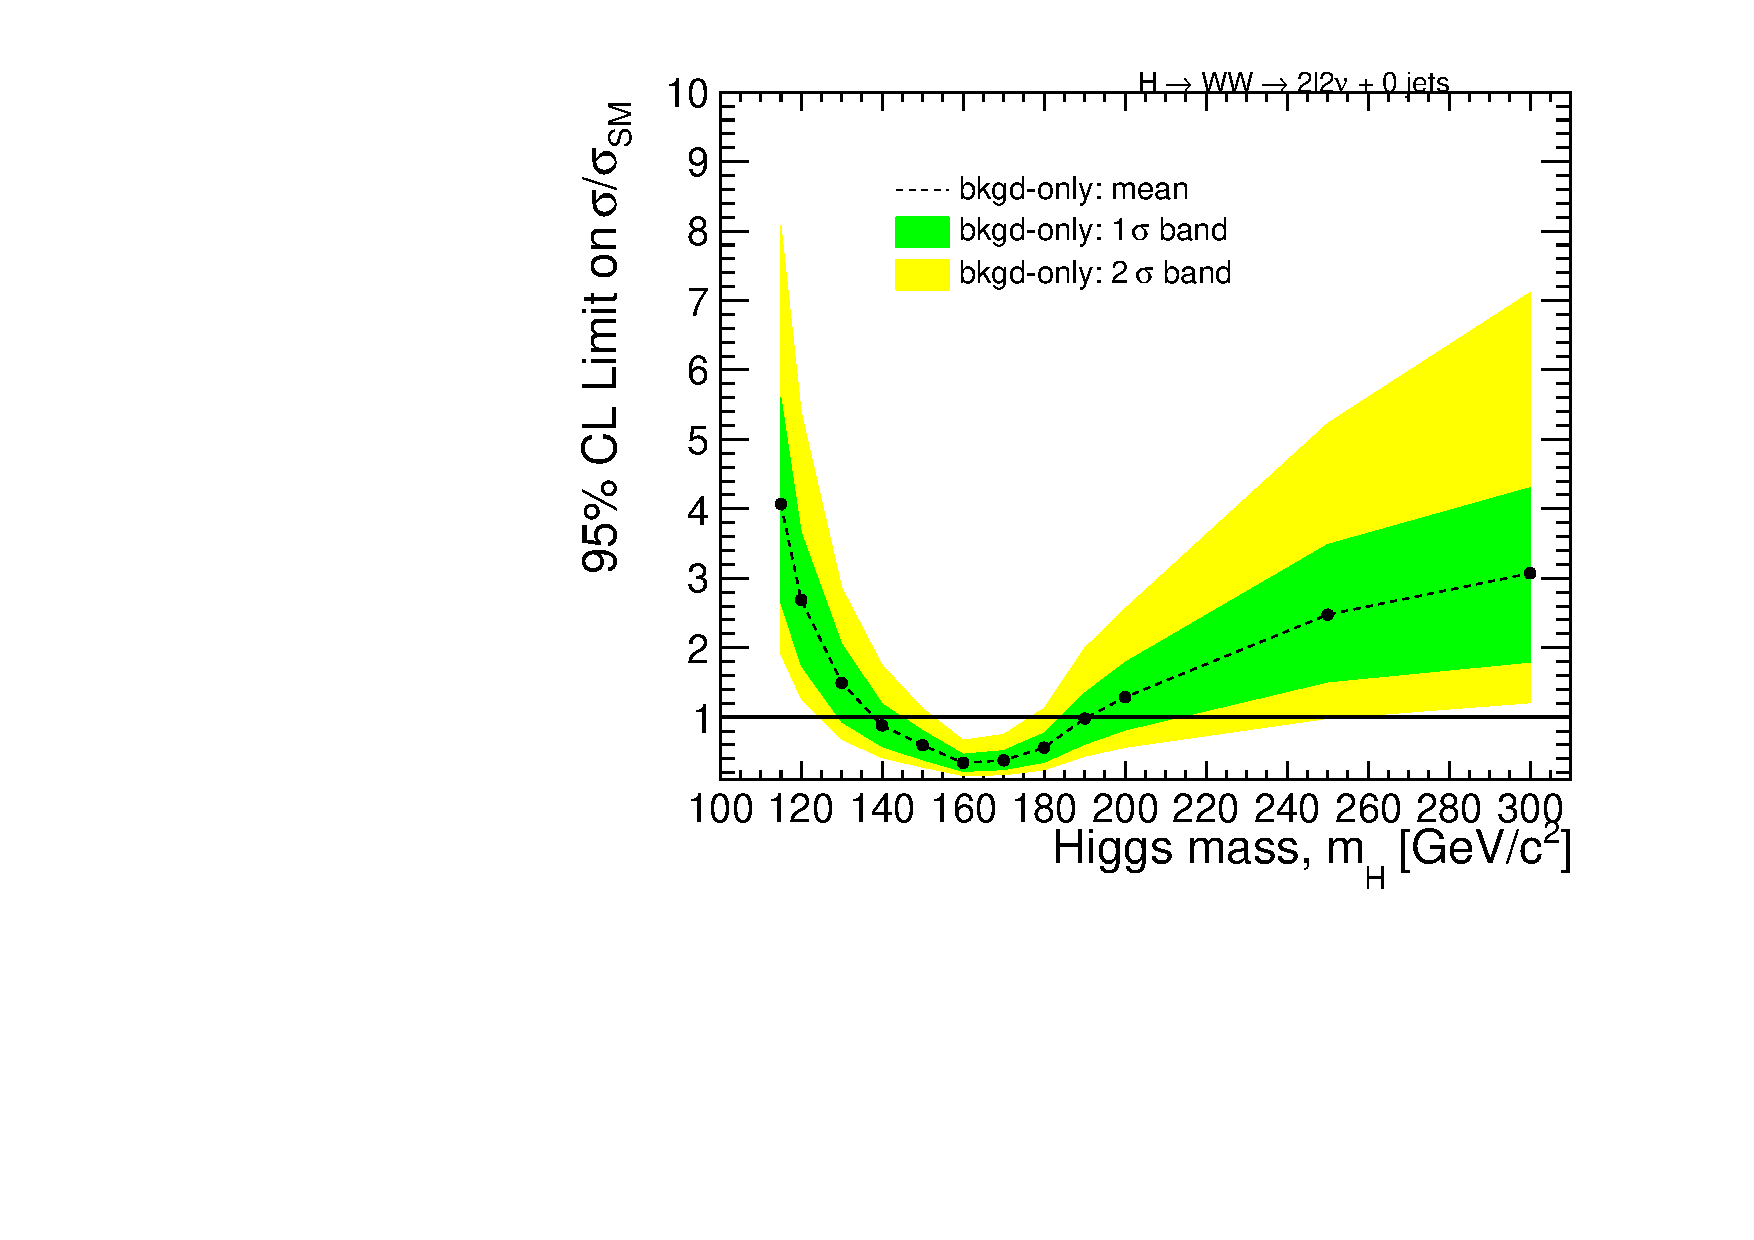
\includegraphics[width=.45\textwidth]{figures/limits_0j_1000pb_ME_shape.pdf}
}
\subfigure[]{
\centering
\label{subfig:bdt_exp_1fb}
%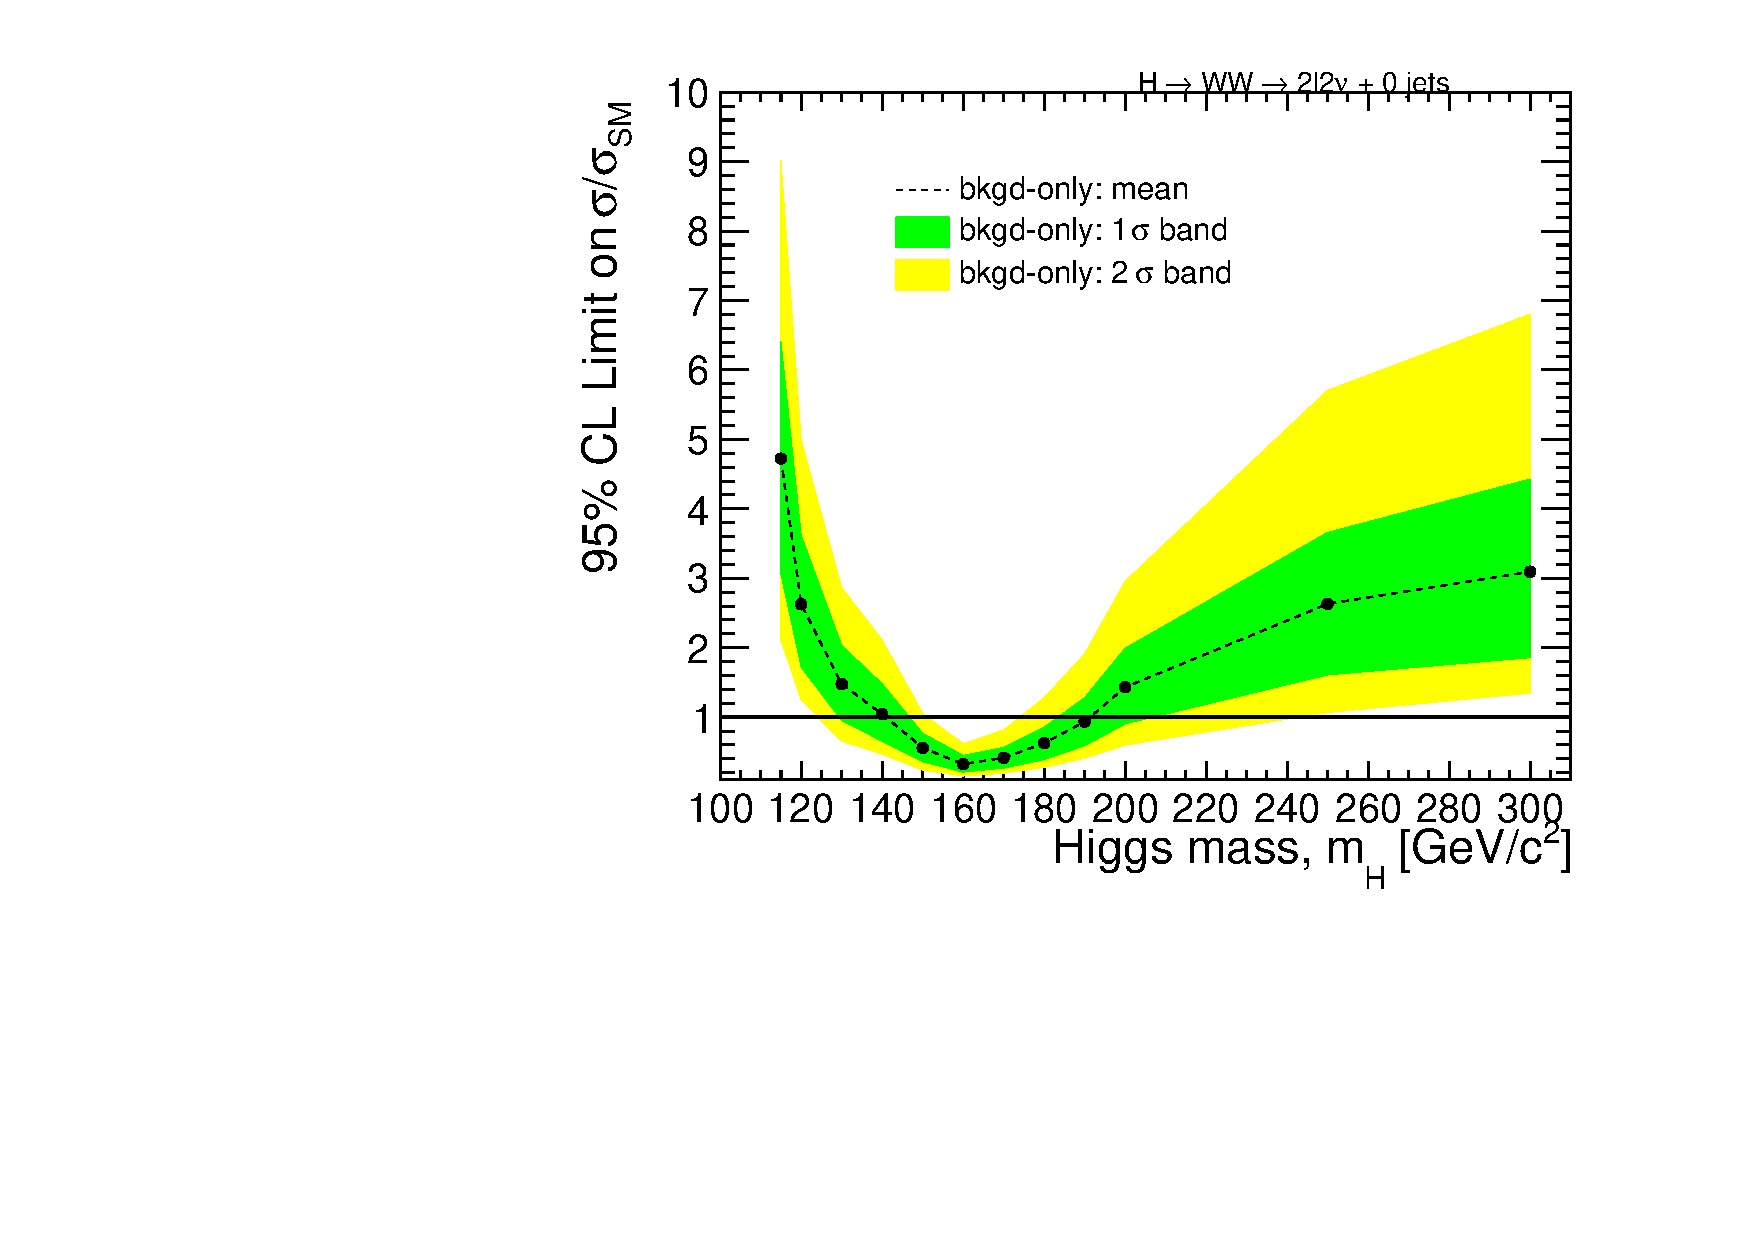
\includegraphics[width=.45\textwidth]{figures/limits_0j_1000pb_BDT_shape.pdf}} \\
}
\caption{ 
Multivariate shape analysis expected upper limits at 95\% C.L. for 1~$\ifb$ data using the 
matrix elemement output \subref{subfig:me_exp_1fb} and BDT output \subref{subfig:bdt_exp_1fb}. } 
\label{fig:me_expected_1fb}
\end{figure}
%%%%%%%%%%%%%%%%%%%%%%%%%%%%%%

%%%%%%%%%%%%%%%%%%%%%%%%%%%%%%
\begin{table}
\begin{center}
\begin{tabular}{c c c c c c c}
\hline\hline
 $m_H$ (GeV) & $-2\sigma$ & $-\sigma$ & median & $+1\sigma$ & $+2\sigma$ \\
\hline
\multicolumn{6}{c} {Matrix Element Method} \\
\hline
 115 & 1.66 & 2.23 &  3.17 &  4.48 &  6.23 \\
 120 & 1.02 & 1.40 &  2.03 &  2.88 &  4.08 \\
 130 & 0.56 & 0.78 &  1.11 &  1.63 &  2.32 \\
 140 & 0.37 & 0.51 &  0.74 &  1.05 &  1.49 \\
 150 & 0.24 & 0.36 &  0.50 &  0.72 &  1.02 \\
 160 & 0.15 & 0.21 &  0.29 &  0.42 &  0.63 \\
 170 & 0.17 & 0.23 &  0.33 &  0.47 &  0.68 \\
 180 & 0.22 & 0.32 &  0.46 &  0.69 &  0.97 \\
 190 & 0.39 & 0.54 &  0.78 &  1.16 &  1.59 \\
 200 & 0.49 & 0.69 &  1.03 &  1.49 &  2.18 \\
 250 & 0.82 & 1.24 &  1.75 &  2.70 &  4.07 \\
 300 & 1.00 & 1.44 &  2.10 &  3.27 &  4.87 \\
\hline
\multicolumn{6}{c} {BDT Based} \\
\hline
 115 & 1.57 & 2.17 &  3.22 &  4.53 &  6.89 \\
 120 & 1.03 & 1.43 &  2.04 &  2.95 &  4.03 \\
 130 & 0.55 & 0.75 &  1.10 &  1.60 &  2.25 \\
 140 & 0.34 & 0.48 &  0.69 &  1.00 &  1.40 \\
 150 & 0.25 & 0.34 &  0.50 &  0.71 &  1.00 \\
 160 & 0.15 & 0.21 &  0.30 &  0.44 &  0.61 \\
 170 & 0.18 & 0.24 &  0.34 &  0.48 &  0.72 \\
 180 & 0.24 & 0.33 &  0.48 &  0.72 &  1.06 \\
 190 & 0.37 & 0.55 &  0.78 &  1.13 &  1.54 \\
 200 & 0.52 & 0.74 &  1.08 &  1.59 &  2.43 \\
 250 & 0.89 & 1.21 &  1.82 &  2.65 &  3.83 \\
 300 & 1.03 & 1.39 &  2.06 &  3.04 &  4.70 \\
\hline\hline
\end{tabular}
\end{center}
\caption{\bf Need to replace with the ZZ results! Multivariate shape analysis expected upper limits at 95\% C.L. for 1~$\ifb$ data using the 
matrix elemement and BDT output corresponding to Figure~\ref{fig:me_expected_1fb}.}
\label{tab:me_expected_1fb}
\end{table}
%%%%%%%%%%%%%%%%%%%%%%%%%%%%%%

  \clearpage

\section{Data Results with $1.1$~$\ifb$}
  \label{sec:dataresults}
  We perform the analysis on a dataset corresponding to $1.1\pm0.1\ifb$ integrated luminosity.

The dilepton $p_T$ distribution is shown in Figure \ref{fig:zpt_zzpresel} after a very loose
cut on the minimum of \met and track \met to be above 20 GeV to take into account data
skimming requirements.  We select events with a dilepton $p_T$ above 40 GeV.
The distribution of the minimum of \met and track \met is shown after the dilepton $p_T$
cut in Figure \ref{fig:minmet_zzpresel}.  The $M_T$ distributions are shown in
Figure \ref{fig:mt_zzpresel} after requiring the minimum of \met and track \met to be 
greater than 50 GeV.  This is referred to as the \zz preselection.

Table~\ref{tab:zzselection_all} shows the number of events observed in
data, comparing to the expected background contribution at the \zz
preselection level. The background estimation was discussed at Section~\ref{sec:backgrounds}.

The Higgs boson mass dependent signal selections are described in Section \ref{sec:signal_selection}.
After applying these signal selections, which differ only from the \zz preselection
in terms of the \met and $M_T$ cuts, the resulting $M_T$ distributions are shown
in Figures \ref{fig:mt_hzz250}, \ref{fig:mt_hzz300} and \ref{fig:mt_hzz400} respectively.

Tables~\ref{tab:yield_hzz250}-\ref{tab:yield_hzz400} show the equivalent data yields
and background expectations.
A more detailed break down of the event yields can be found in ~\ref{app:yield1fbdetail}.

%%%%%%%%
\begin{table}[!ht]
\begin{center}
\begin{tabular} {c|c|c|cccccc}
\hline
  & data & all bkg. & $\dyll$ & $\ZZ$ & $\WZ$ & $WW$ & $\ttbar+tW$ & $\Wjets$  \\
\hline
\multicolumn{9}{c} {0 Jet Bin} \\
\hline
 $\mu\mu$ &  39 & $43.4\pm0.9$ & $8.2\pm0.1$ & $14.5\pm0.3$ & $7.1\pm0.3$ & $11.6\pm0.4$ & $2.1\pm0.7$ & $0.0$ \\
 $ee$     &  31 & $31.7\pm0.8$ & $8.2\pm0.1$ & $9.7\pm0.2$  & $4.0\pm0.2$ & $7.5\pm0.3$ & $1.0\pm0.3$ & $1.3\pm0.6$ \\
\hline
\multicolumn{9}{c} {1 Jet Bin} \\
\hline
 $\mu\mu$ &  21 & $22.6\pm0.8$ & $8.8\pm0.1$ & $3.7\pm0.1$ & $3.7\pm0.2$ &  $3.3\pm0.2$ & $3.1\pm0.7$ & $0.0$  \\
 $ee$     &  18 & $19.6\pm0.9$ & $8.8\pm0.1$ & $2.6\pm0.1$ & $2.5\pm0.2$ & $2.2\pm0.2$ & $3.6\pm0.8$ & $0.0$ \\
\hline
\end{tabular}
\caption{Expected number of signal and background events from the data-driven methods for an 
  integrated luminosity of \intlumi  after applying the $\ZZ$ selection requirements. 
Only statistical uncertaities are reported. }
   \label{tab:zzselection_all}
  \end{center}
\end{table}
%%%%%%%%

%%%%%%%%
%\begin{table}[!ht]
%\begin{center}
%\begin{tabular} {c|c|c|c|ccccc}
%\hline
%  & data & $HZZ$(200) & all bkg. & $\dyll$ & $\ZZ$ & $\WZ$ & $WW$ & $\ttbar+tW$ \\
%\hline
%\multicolumn{9}{c} {0 Jet Bin} \\
%\hline
% $\mu\mu$ &  12 & $0.12\pm0.01$ & $13.9\pm0.4$ & $3.34\pm0.04$ & $3.1\pm0.1$ & $2.1\pm0.2$ & $4.8\pm0.2$ & $0.5\pm0.3$ \\
% $ee$     &  14 & $0.07\pm0.01$ & $9.9\pm0.3$  & $3.34\pm0.04$ & $2.0\pm0.1$ & $1.2\pm0.1$ & $3.1\pm0.2$ & $0.2\pm0.2$ \\
%\hline
%\multicolumn{9}{c} {1 Jet Bin} \\
%\hline
% $\mu\mu$ &  0 & $0.02\pm0.00$ & $0.34\pm0.10$ & $0.12\pm0.01$ & $0.02\pm0.01$ & $0.01\pm0.01$ & $0.07\pm0.03$ & $0.13\pm0.09$ \\
% $ee$     &  0 & $0.01\pm0.00$ & $0.20\pm0.03$ & $0.12\pm0.01$ & $0.01\pm0.01$ & $0.02\pm0.01$ & $0.05\pm0.02$ & $0.0$ \\
%\hline
%\end{tabular}
%\caption{Expected number of signal and background events from the data-driven methods for an 
%  integrated luminosity of \intlumi  after applying the $\hzz$ ($m_H=200\GeVcc$) selection requirements. 
%Only statistical uncertaities are reported. The $\Wjets$ background is neglible thus omitted in the table.}
%   \label{tab:yield_hzz200}
%  \end{center}
%\end{table}
%%%%%%%%


%%%%%%%%
\begin{table}[!ht]
\begin{center}
\begin{tabular} {c|c|c|c|ccccc}
\hline
  & data & $HZZ$(250) & all bkg. & $\dyll$ & $\ZZ$ & $\WZ$ & $WW$ & $\ttbar+tW$ \\
\hline
\multicolumn{9}{c} {0 Jet Bin} \\
\hline
 $\mu\mu$ &  20 & $2.12\pm0.04$ & $16.7\pm0.7$ & $3.4\pm0.1$ & $5.3\pm0.2$ & $2.7\pm0.2$ & $4.0\pm0.2$ & $1.4\pm0.0.6$ \\
 $ee$     &  7 & $1.57\pm0.03$ & $12.7\pm0.6$ & $3.4\pm0.1$ & $3.5\pm0.1$ & $1.6\pm0.1$ & $2.9\pm0.2$ & $0.5\pm0.2$ \\
\hline
\multicolumn{9}{c} {1 Jet Bin} \\
\hline
 $\mu\mu$ &  5 & $1.02\pm0.02$ & $9.1\pm0.6$ & $2.38\pm0.02$ & $1.4\pm0.1$ & $1.8\pm0.2$ & $1.7\pm0.1$ & $1.8\pm0.5$ \\
 $ee$     &  8 & $0.70\pm0.02$ & $8.6\pm0.8$ & $2.38\pm0.02$ & $1.1\pm0.1$ & $1.1\pm0.1$ & $1.2\pm0.1$ & $2.9\pm0.8$ \\
\hline
\end{tabular}
\caption{Expected number of signal and background events from the data-driven methods for an 
  integrated luminosity of \intlumi  after applying the $\hzz$ ($m_H=250\GeVcc$) selection requirements. 
Only statistical uncertaities are reported. The $\Wjets$ background is neglible thus omitted in the table.}
   \label{tab:yield_hzz250}
  \end{center}
%\end{table}
%%%%%%%%
%%%%%%%%
%\begin{table}[!ht]
\begin{center}
\begin{tabular} {c|c|c|c|ccccc}
\hline
  & data & $HZZ$(300) & all bkg. & $\dyll$ & $\ZZ$ & $\WZ$ & $WW$ & $\ttbar+tW$ \\
\hline
\multicolumn{9}{c} {0 Jet Bin} \\
\hline
 $\mu\mu$ &  3 & $1.67\pm0.03$ & $5.4\pm0.2$ & $0.26\pm0.03$ & $2.9\pm0.1$ & $1.3\pm0.1$ & $0.8\pm0.1$ & $0.09\pm0.0.05$ \\
 $ee$     &  4 & $1.18\pm0.02$ & $3.6\pm0.2$ & $0.26\pm0.03$ & $2.2\pm0.1$ & $0.6\pm0.1$ & $0.4\pm0.1$ & $0.14\pm0.14$ \\
\hline
\multicolumn{9}{c} {1 Jet Bin} \\
\hline
 $\mu\mu$ &  1 & $0.60\pm0.01$ & $1.3\pm0.2$ & $0.16\pm0.01$ & $0.47\pm0.05$ & $0.26\pm0.06$ & $0.14\pm0.04$ & $0.25\pm0.22$ \\
 $ee$     &  2 & $0.43\pm0.01$ & $0.9\pm0.1$ & $0.16\pm0.01$ & $0.34\pm0.04$ & $0.15\pm0.04$ & $0.13\pm0.03$ & $0.08\pm0.08$ \\
\hline
\end{tabular}
\caption{Expected number of signal and background events from the data-driven methods for an  
integrated luminosity of \intlumi  after applying the $\hzz$ ($m_H=300\GeVcc$) selection requirements. 
Only statistical uncertaities are reported. The $\Wjets$ background is neglible thus omitted in the table.}
   \label{tab:yield_hzz300}
  \end{center}
%\end{table}
%%%%%%%%
%%%%%%%%
%\begin{table}[!ht]
\begin{center}
\begin{tabular} {c|c|c|c|ccccc}
\hline
  & data & $HZZ$(400) & all bkg. & $\dyll$ & $\ZZ$ & $\WZ$ & $WW$ & $\ttbar+tW$ \\
\hline
\multicolumn{9}{c} {0 Jet Bin} \\
\hline
 $\mu\mu$ &  1 & $1.29\pm0.02$ & $2.3\pm0.1$ & $0.0$ & $1.7\pm0.1$ & $0.55\pm0.08$ & $0$ & $0$ \\
 $ee$     &  2 & $0.94\pm0.02$ & $1.4\pm0.1$ & $0.0$ & $1.1\pm0.1$ & $0.25\pm0.06$ & $0$ & $0$ \\
\hline
\multicolumn{9}{c} {1 Jet Bin} \\
\hline
 $\mu\mu$ &  2 & $0.97\pm0.02$ & $1.5\pm0.1$ & $0.43\pm0.05$ & $0.68\pm0.06$ & $0.37\pm0.07$ & $0.05\pm0.02$ & $0$ \\
 $ee$     &  3 & $0.70\pm0.01$ & $1.1\pm0.1$ & $0.43\pm0.05$ & $0.46\pm0.05$ & $0.21\pm0.05$ & $0.04\pm0.01$ & $0$ \\
\hline
\end{tabular}
\caption{Expected number of signal and background events from the data-driven methods for an 
integrated luminosity of \intlumi  after applying the $\hzz$ ($m_H=400\GeVcc$) selection requirements. 
Only statistical uncertaities are reported. The $\Wjets$ background is neglible thus omitted in the table.}
   \label{tab:yield_hzz400}
  \end{center}
\end{table}
%%%%%%%%


%%%%%%%%
\begin{figure}[!hbtp]
\begin{center}
\label{fig:zpt_zzpresel}
\subfigure[0-Jet]{\label{subfig:zpt_0j}
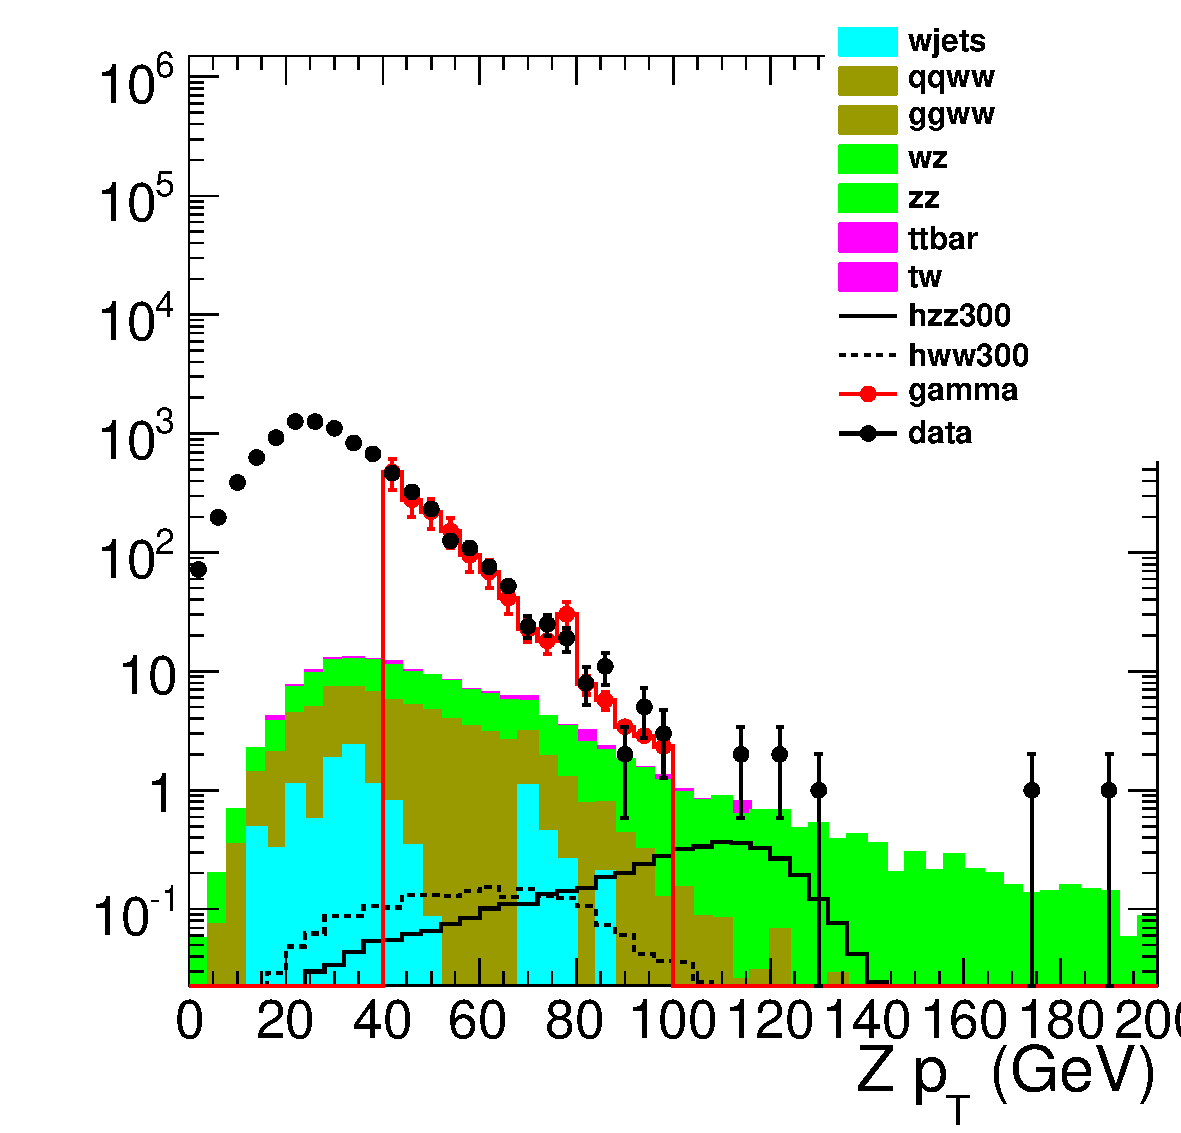
\includegraphics[width=.3\textwidth]{figures/presel_hzz300_zpt_0j_log.pdf}}
\subfigure[1-Jet]{\label{subfig:zpt_1j}
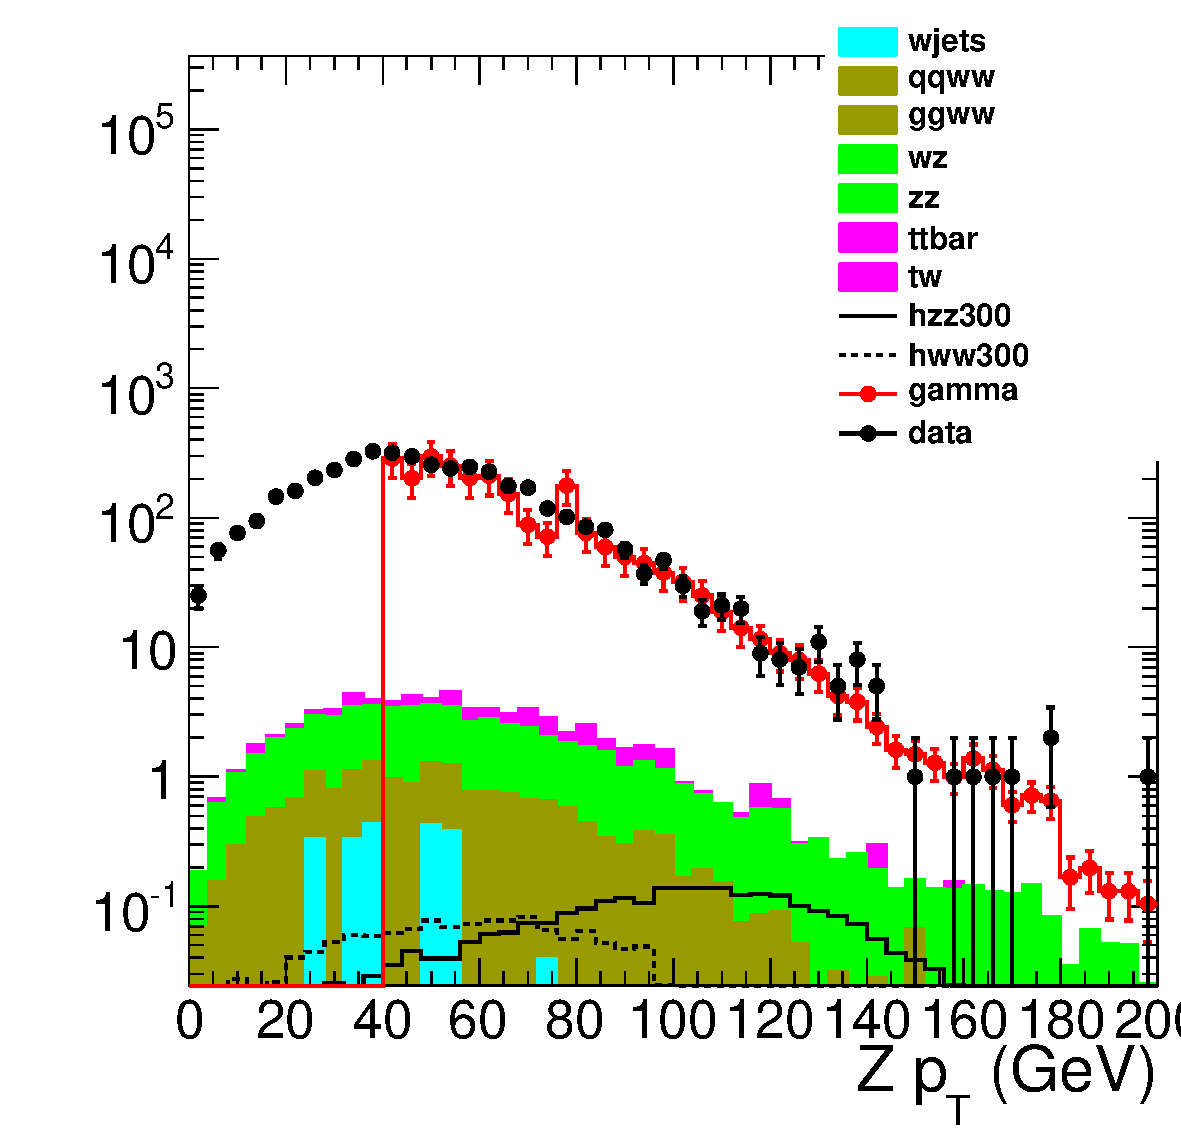
\includegraphics[width=.3\textwidth]{figures/presel_hzz300_zpt_1j_log.pdf}}
\subfigure[$\geq$2 Jets]{\label{subfig:zpt_2j}
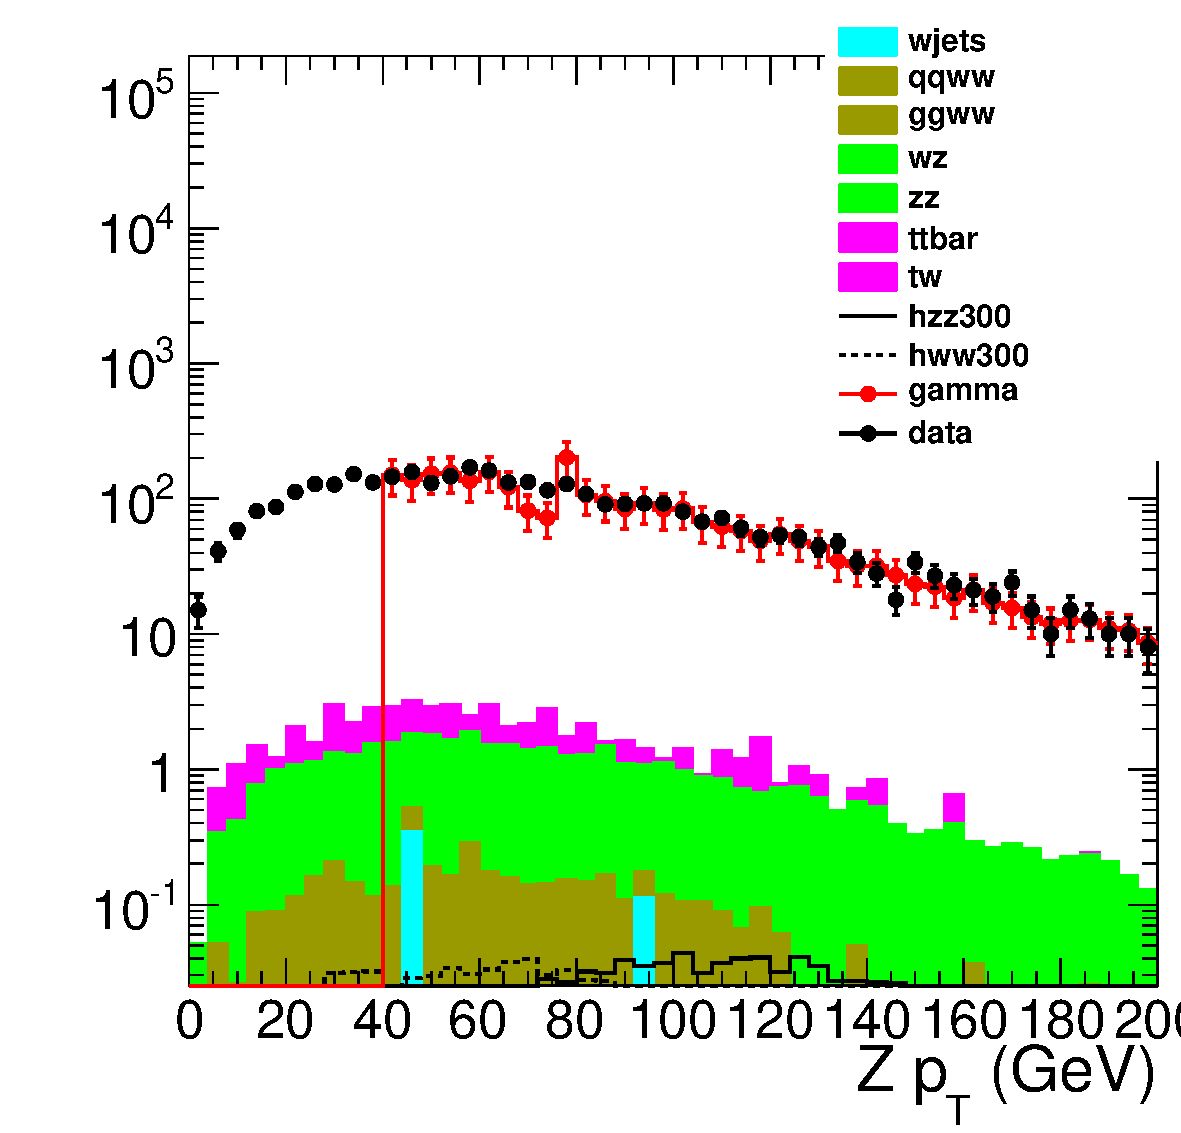
\includegraphics[width=.3\textwidth]{figures/presel_hzz300_zpt_2j_log.pdf}}
\caption{Dilepton $p_T$ distribution after the $\ZZ$ preselection observed in data corresponding to $1092\pm7$~\ipb data in 0-Jet~\subref{subfig:zpt_0j}, 1-Jet~\subref{subfig:zpt_1j}
and 2-Jet~\subref{subfig:zpt_2j} bins, compared to the expected from simulation for signal and background.
The MC backgrounds are scaled as appropriate and the photon+jets estimate of the Z+jets background is added to the stack.}
\end{center}
\end{figure}
%%%%%%%%

%%%%%%%%
\begin{figure}[!hbtp]
\begin{center}
\label{fig:minmet_zzpresel}
\subfigure[0-Jet]{\label{subfig:minmet_0j}
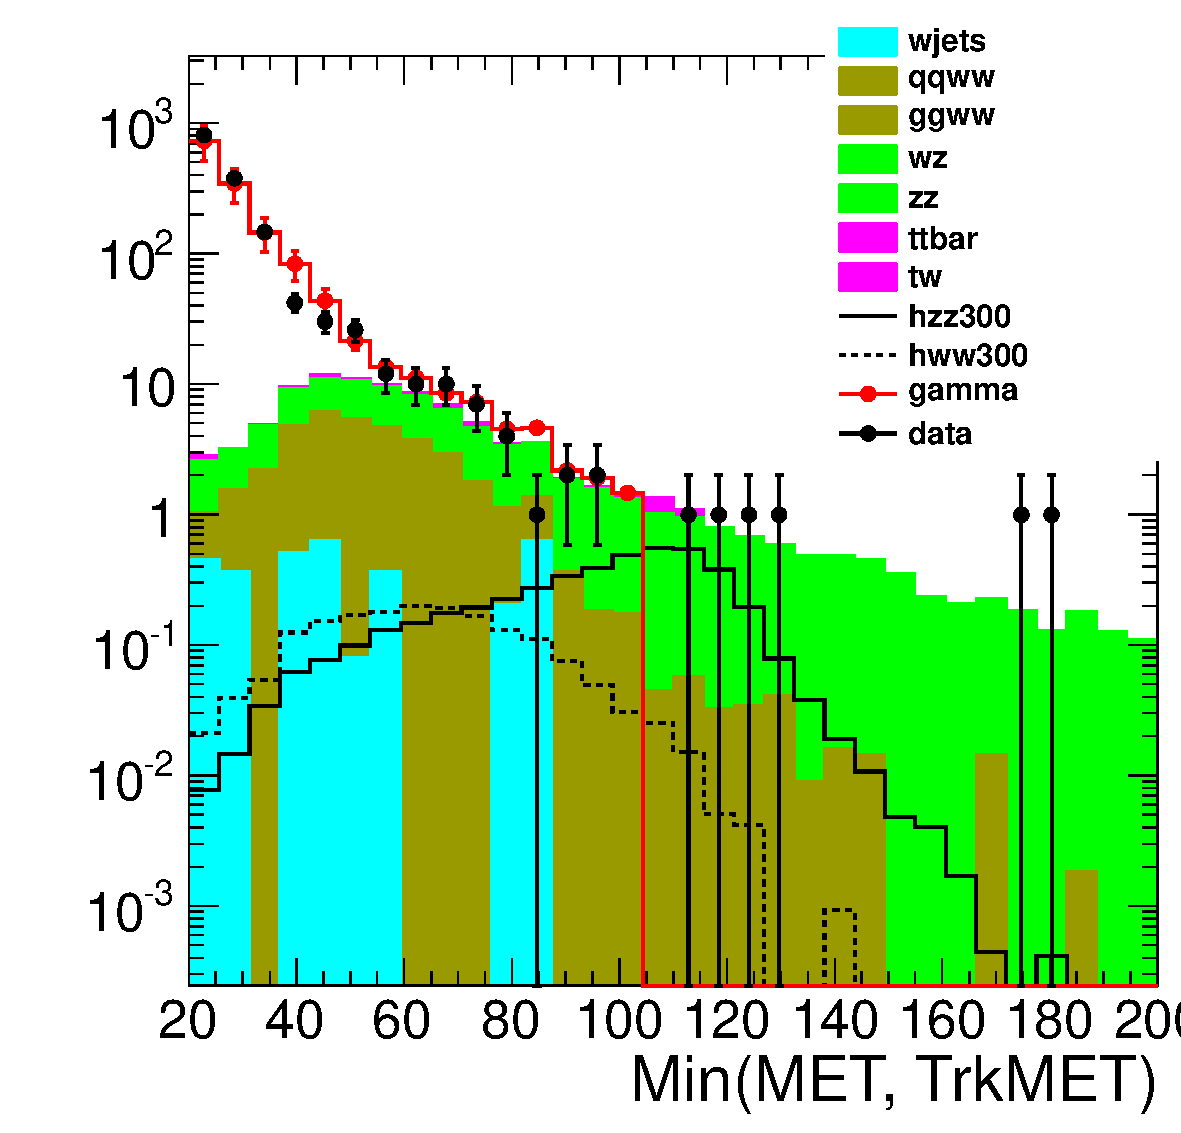
\includegraphics[width=.3\textwidth]{figures/presel_hzz300_minmet_0j_log.pdf}}
\subfigure[1-Jet]{\label{subfig:minmet_1j}
\includegraphics[width=.3\textwidth]{figures/presel_hzz300_minmet_1j_log.pdf}}
\subfigure[$\geq$2 Jets]{\label{subfig:minmet_2j}
\includegraphics[width=.3\textwidth]{figures/presel_hzz300_minmet_2j_log.pdf}}
\caption{Min-MET distribution after the $\ZZ$ preselection observed in data corresponding to $1092\pm7$~\ipb data in 0-Jet~\subref{subfig:minmet_0j}, 1-Jet~\subref{subfig:minmet_1j} 
and 2-Jet~\subref{subfig:minmet_2j} bins, compared to the expected from simulation for signal and background. 
The MC backgrounds are scaled as appropriate and the photon+jets estimate of the Z+jets background is added to the stack.}
\end{center}
\end{figure}
%%%%%%%%


%%%%%%%%
\begin{figure}[!hbtp]
\begin{center}
\label{fig:mt_zzpresel}
\subfigure[0-Jet]{\label{subfig:mt_0j}
\includegraphics[width=.3\textwidth]{figures/presel_hzz300_mt_0j.pdf}}
\subfigure[1-Jet]{\label{subfig:mt_1j}
\includegraphics[width=.3\textwidth]{figures/presel_hzz300_mt_1j.pdf}}
\subfigure[$\geq$2 Jets]{\label{subfig:mt_2j}
\includegraphics[width=.3\textwidth]{figures/presel_hzz300_mt_2j.pdf}}
\caption{Transverse mass $m_T$ distribution after the $\ZZ$ preselection observed in data corresponding to $1092\pm7$~\ipb data in 0-Jet~\subref{subfig:mt_0j}, 1-Jet~\subref{subfig:mt_1j} 
and 2-Jet~\subref{subfig:mt_2j} bins, compared to the expected from simulation for signal and background. 
The MC backgrounds are scaled as appropriate and the photon+jets estimate of the Z+jets background is added to the stack.}
\end{center}
\end{figure}
%%%%%%%%

%%%%%%%%
\begin{figure}[!hbtp]
\begin{center}
\label{fig:mt_hzz250}
\subfigure[0-Jet]{\label{subfig:mt_0j}
\includegraphics[width=.3\textwidth]{figures/hzz250_mt_0j.pdf}}
\subfigure[1-Jet]{\label{subfig:mt_1j}
\includegraphics[width=.3\textwidth]{figures/hzz250_mt_1j.pdf}}
\caption{Transverse mass $m_T$ distribution after the full $\hzz$ ($m_H = 250\GeVcc$) selection observed in 
data corresponding to $1092\pm7$~\ipb data in 0-Jet~\subref{subfig:mt_0j} and 1-Jet~\subref{subfig:mt_1j}
bins compared to the expected from simulation for signal and background. 
The MC backgrounds are scaled as appropriate and the photon+jets estimate of the Z+jets background is added to the stack.}
\end{center}
\end{figure}
%%%%%%%%

%%%%%%%%
\begin{figure}[!hbtp]
\begin{center}
\label{fig:mt_hzz300}
\subfigure[0-Jet]{\label{subfig:mt_0j}
\includegraphics[width=.3\textwidth]{figures/hzz300_mt_0j.pdf}}
\subfigure[1-Jet]{\label{subfig:mt_1j}
\includegraphics[width=.3\textwidth]{figures/hzz300_mt_1j.pdf}}
\caption{Transverse mass $m_T$ distribution after the full $\hzz$ ($m_H = 300\GeVcc$) selection observed in
data corresponding to $1092\pm7$~\ipb data in 0-Jet~\subref{subfig:mt_0j} and 1-Jet~\subref{subfig:mt_1j}
bins compared to the expected from simulation for signal and background. 
The MC backgrounds are scaled as appropriate and the photon+jets estimate of the Z+jets background is added to the stack.}
\end{center}
\end{figure}
%%%%%%%%

%%%%%%%%
\begin{figure}[!hbtp]
\begin{center}
\label{fig:mt_hzz400}
\subfigure[0-Jet]{\label{subfig:mt_0j}
\includegraphics[width=.3\textwidth]{figures/hzz400_mt_0j.pdf}}
\subfigure[1-Jet]{\label{subfig:mt_1j}
\includegraphics[width=.3\textwidth]{figures/hzz400_mt_1j.pdf}}
\caption{Transverse mass $m_T$ distribution after the full $\hzz$ ($m_H = 400\GeVcc$) selection observed in
data corresponding to $1092\pm7$~\ipb data in 0-Jet~\subref{subfig:mt_0j} and 1-Jet~\subref{subfig:mt_1j}
bins compared to the expected from simulation for signal and background. 
The MC backgrounds are scaled as appropriate and the photon+jets estimate of the Z+jets background is added to the stack.}
\end{center}
\end{figure}
%%%%%%%%


\clearpage

\section{Summary}
    \label{sec:summary}
    
We have performed a measurement of the $W^+W^-$ production cross-section
using an integrated luminosity of $\intlumi$ of $pp$ collision data at $\sqrt{s} = $
7~$\TeV$. The measurement was performed in the \wwlnln{} final state.
The $W^+W^-$ production cross-section was measured to be:

\begin{equation*}
\sigma_{WW}  = 53.95 \pm 2.05~\mathrm{(stat.)} \pm 4.30~\mathrm{(syst.)} \pm 2.43~\mathrm{(lumi.)~pb},
\end{equation*}

to be compared with the standard model prediction \cite{Campbell:2011bn}:

\begin{equation*}
\sigma_{WW}  = 47 \pm 2 ~\mathrm{pb}.
\end{equation*}



\clearpage
%===================================================================================================
\clearpage

\vspace*{-0.2cm}
\thebibliography{12}

\bibitem{pdg}
 K. Nakamura et al. (Particle Data Group), "Review of particle physics", J. Phys.G37 , 2010.

\bibitem{Higgs1}
F. Englert and R. Brout, "Broken symmetries and the masses of gauge bosons", Phys. Rev. Lett. 13,  1964.

\bibitem{Higgs2}
P. W. Higgs, "Broken symmetry and the mass of gauge vector mesons", Phys. Rev. Lett. 13, 1964.

\bibitem{Higgs3}
Guralnik, G.S. and Hagen, C.R. and Kibble, T.W.B., "Global Conservation Laws and Massless Particles", 
Phys.Rev.Lett. 13, 1964.

\bibitem{dittmar}
M.~Dittmar and H.~K.~Dreiner, Phys.\ Rev.\  D {\bf 55} (1997) 167".

\bibitem{HWW2010}
CMS Collaboration, "Measurement of WW Production and Search for the Higgs Boson in 
pp Collisions at $\sqrt{s}$ = 7 TeV", arXiv:1102.5429

\bibitem{HWW2011AN}
L.~Bauerdick et al, "A Higgs Boson Search in the Fully Leptonic $W^+W^-$ Final State", CMS AN-2011/155

\bibitem{VBTFCrossSectionNote}
J. Alcaraz Maestre, \textit{et al.}, "Updated Measurements of Inclusive W and Z Cross Sections 
at $\sqrt{s}=7$ TeV", CMS AN-2010/264.

\bibitem{ggWWError}
F.~ Stoeckli, "http://indico.cern.ch/getFile.py/access?contribId=0\&resId=1\&materialId=slides\&confId=49009", 
EWK Diboson meeting of March 12 2009.

\bibitem{json}
{\small
/afs/cern.ch/cms/CAF/CMSCOMM/COMM\_DQM/certification/Collisions11/7TeV/Prompt/Cert\_160404-163869\_7TeV\_PromptReco\_Collisions11\_JSON.txt
}

\bibitem{ElIso}
A. Vartak, M. LeBourgeois, V. Sharma, "Lepton Isolation in the CMS Tracker, ECAL and HCAL", CMS AN-2010/106.

\bibitem{PVDA}
W. Erdmann, M. LeBourgeois, B. Mangano, 
https://indico.cern.ch/getFile.py/access?contribId=5\&sessionId=3\&resId=1\&materialId=slides\&confId=127127, 
note in preparation.

\bibitem{NExpHits}
B. Mangano \textit{et al.}, "Improvement in Photon Conversion Rejection Performance Using 
Advanced Tracking Tools", AN-10-283.

\bibitem{fakeLeptonNote1}
S.~Xie, \textit{et al.}", "Study of Data-Driven Methods for Estimation of Fake Lepton Backgrounds", 
CMS AN-2009/120.

\bibitem{fakeLeptonNote2}
W.~Andrews, \textit{et al.}, "Fake Rates for dilepton Analyses", CMS AN-2010/257.

\bibitem{fakeLeptonBkgSpillage1}
 F. Golf, D. Evans, J. Mulmenstadt  \textit{et al.}, ``Expectations for observation of top quark pair production in the dilepton final state with the early CMS data'', CMS AN-2009/050.

\bibitem{dyestnote}
W. Andrews, et al., “A Method to Measure the Contribution of $\dyll$ to a di-lepton+ MET Selection”, CMS AN-2009/023 (2009).

\bibitem{jes}
CMS Collaboration, "Jet Energy Calibration with Photon+Jet Events", PAS JME-09-004.

\bibitem{jetpas}
CMS Collaboration, "Jet Performance in pp Collisions at $\sqrt{s}=7 \rm\ TeV$", PAS JME-10-003.

\bibitem{btag}
CMS collaboration, "Commissioning of b-jet identification with pp collisions at $\sqrt{s}=7~\TeV$, BTV-10-001.

\bibitem{antikt}
Cacciari, Matteo and Salam, Gavin P. and Soyez, Gregory, "The anti-$k_t$ jet clustering 
algorithm", JHEP 04,  2008.

\bibitem{ConversionNote}
W.~Andrews, \textit{et al.}, "Study of photon conversion rejection at CMS", CMS AN-2009/159.

\bibitem{tmva}
A. Hoecker, \textit{et al.}, "TMVA - Toolkit for Multivariate Data Analysis", arXiv:physics/0703039, 2007.

\bibitem{XS}
CMS Generator group, Standard Model Cross Sections for CMS at 7 TeV, 2010.

\bibitem{PDF4LHC}
PDF4LHC Working Group, 
{\tt http://www.hep.ucl.ac.uk/pdf4lhc/PDF4LHCrecom.pdf}

\bibitem{Nadolsky:2008zw}
Nadolsky, Pavel M. and others, "Implications of CTEQ global analysis for 
collider observables", Phys. Rev. D78 2008.

\bibitem{Martin:2009iq}
Martin, A. D. and Stirling, W. J. and Thorne, R. S. and Watt, G., "Parton 
distributions for the LHC, Eur. Phys. J. C63 2009.

\bibitem{Ball:2010de}
Ball, Richard D. and others, "A first unbiased global NLO determination 
of parton distributions and their uncertainties", arXiv 1002.4407.

\bibitem{bayesian}
A. O'Hagan and J.J. Forster, "Bayesian Inference", Kendall's Advanced Theory of Statistics, 
Arnold, London, 2B, 2004.

\bibitem{ref:tagprobe_mit_w}
G. Bauer {\it et. al.}, "Lepton ef?iencies for the inclusive W cross section measurement with 36.1pb$^{-1}$", AN2011/097

\bibitem{ref:tagprobe_snt_top}
W. Andrews {\it et. al.}, "Uncertainties on the Lepton Selection Efficiency for t$t\bar{t}$ Cross Section Analysis", AN2010/274

\bibitem{LHCHiggsCrossSectionWorkingGroup:2011ti}
LHC Higgs Cross Section Working Group, "Handbook of LHC Higgs Cross Sections: 
Inclusive Observables", CERN-2011-002, 2011.

\bibitem{PFMET} 
CMS Collaboration, ``CMS MET Performance in Events Containing Electroweak Bosons from pp Collisions at $\sqrt{s}=7$ TeV'', CMS PAS JME-2010-005 (2010)


\bibitem{trkMET} 
Marco Zanetti, ``MET with PU in $\hww\to2\ell$'', https://indico.cern.ch/conferenceDisplay.py?confId=131580
Benjamin Hooberman, ``MET with PU in MC and First 2011 Data'', https://indico.cern.ch/contributionDisplay.py?contribId=5\&confId=132579. 


\bibitem{lands}
Mingshui Chen and Andrey Korytov, https://mschen.web.cern.ch/mschen/lands/

\bibitem{MCFMHiggsProduction}
J. Campbell, R.K. Ellis, G. Zanderighi, ``Next-to-Leading order Higgs + 2 jet production via gluon fusion.'', JHEP 0610:028 (2006), hep-ph/0608194

\bibitem{MCFMVVProduction}
J. Campbell, R.K. Ellis, C. Williams, ``Vector boson pair production at the LHC.'', arxiv:hep-ph/1105.0020.

\bibitem{MITHggNote} 
G. Bauer et al., ``Higgs Search in the pp $\rightarrow$ H $\rightarrow$ $\gamma\gamma$ channel at $\sqrt{s}=7$ TeV'', CMS AN-2011/168. 



%===================================================================================================

\clearpage
\appendix

\section{Cross-check of the EPS Analysis}
\label{app:xcheckeps}
In this section we document the results obtained using the selections 
documented  in the Ref.~\cite{HZZ2011EPS} and \cite{HZZ2011EPSPAS}. 


\clearpage
%\section{Event Yields for 1~\ifb data}
%\label{app:yield1fbdetail}
%%%%%%%%%
\begin{table}[!ht]
\begin{center}
\begin{tabular}{c|cc|c}
\hline
sample    & $\mu\mu$   & ee     & TOTAL\\ \hline 
\multicolumn{4}{c} { 0 Jet Bin} \\
\hline
$\Wjets$   & 0.00 $\pm$ 0.00   & 1.29 $\pm$ 0.63   & 1.29 $\pm$ 0.63 \\  
\qqww   & 10.91 $\pm$ 0.35   & 7.09 $\pm$ 0.27   & 17.99 $\pm$ 0.45 \\  
\ggww   & 0.68 $\pm$ 0.04   & 0.46 $\pm$ 0.03   & 1.14 $\pm$ 0.05 \\  
\wz   & 7.12 $\pm$ 0.30   & 4.03 $\pm$ 0.22   & 11.15 $\pm$ 0.37 \\  
$\ZZ$   & 14.54 $\pm$ 0.28   & 9.67 $\pm$ 0.22   & 24.21 $\pm$ 0.35 \\  
$\ttbar$   & 1.44 $\pm$ 0.63   & 0.41 $\pm$ 0.25   & 1.85 $\pm$ 0.67 \\  
$\tw$   & 0.63 $\pm$ 0.16   & 0.58 $\pm$ 0.15   & 1.21 $\pm$ 0.22 \\  
$\dytt$   & 0.00 $\pm$ 0.00   & 0.00 $\pm$ 0.00   & 0.00 $\pm$ 0.00 \\  
$\dyll$   & 8.17 $\pm$ 0.10   & 8.17 $\pm$ 0.10   & 16.34 $\pm$ 0.15 \\  
\hline
Background   & 43.49 $\pm$ 0.85   & 31.70 $\pm$ 0.81   & 75.18 $\pm$ 1.17 \\  
\hline
DATA   & 39.00 $\pm$ 6.24   & 31.00 $\pm$ 5.57   & 70.00 $\pm$ 8.37 \\ 
\hline
hzz300   & 2.50 $\pm$ 0.03   & 1.75 $\pm$ 0.03   & 4.25 $\pm$ 0.04 \\  
hww300   & 0.74 $\pm$ 0.03   & 0.55 $\pm$ 0.02   & 1.29 $\pm$ 0.04 \\  
\hline 
\multicolumn{4}{c} { 1 Jet Bin} \\
\hline
$\Wjets$   & 0.00 $\pm$ 0.00   & 0.00 $\pm$ 0.00   & 0.00 $\pm$ 0.00 \\  
\qqww   & 3.11 $\pm$ 0.18   & 2.04 $\pm$ 0.14   & 5.15 $\pm$ 0.23 \\  
\ggww   & 0.21 $\pm$ 0.02   & 0.14 $\pm$ 0.02   & 0.34 $\pm$ 0.03 \\  
\wz   & 3.74 $\pm$ 0.22   & 2.50 $\pm$ 0.17   & 6.24 $\pm$ 0.28 \\  
\zz   & 3.68 $\pm$ 0.14   & 2.59 $\pm$ 0.11   & 6.27 $\pm$ 0.18 \\  
$\ttbar$  & 2.35 $\pm$ 0.70   & 2.77 $\pm$ 0.81   & 5.11 $\pm$ 1.07 \\  
\tw   & 0.72 $\pm$ 0.15   & 0.82 $\pm$ 0.17   & 1.54 $\pm$ 0.23 \\  
$\dytt$   & 0.00 $\pm$ 0.00   & 0.00 $\pm$ 0.00   & 0.00 $\pm$ 0.00 \\  
$\dyll$  & 8.79 $\pm$ 0.11   & 8.79 $\pm$ 0.11   & 17.57 $\pm$ 0.15 \\  
\hline
Background   & 22.59 $\pm$ 0.79   & 19.63 $\pm$ 0.87   & 42.22 $\pm$ 1.17 \\  
hzz300   & 1.42 $\pm$ 0.02   & 0.98 $\pm$ 0.02   & 2.40 $\pm$ 0.03 \\  
\hline
DATA   & 21.00 $\pm$ 4.58   & 18.00 $\pm$ 4.24   & 39.00 $\pm$ 6.24 \\ 
\hline
\end{tabular}
\caption{
Expected number of signal and background events from the data-driven methods for an 
  integrated luminosity of \intlumi  after the {\bf $\ZZ$ pre-selection in the 0/1-Jet bin}. 
Only statistical uncertainties are reported. The MC expectations includes the lepton efficiencies, 
trigger efficiencies, pileup reweighting, 
higher order reweighting on the $\hzz$ and $\pt$-dependent reweighting on $\ZZ$. The $\ttbar$, 
$\tw$, $\ww$, $\dytt$ and $\Wjets$ yields include the data/MC scale factors derived in section~\ref{sec:backgrounds}. }
\label{tab:yield_zzpresel}
\end{center}
\end{table}
%%%%%%%%


%%%%%%%%
\begin{table}[!ht]
\begin{center}
\begin{tabular}{c|cc|c}
\hline
sample    & $\mu\mu$   & ee     & TOTAL\\ \hline 
\multicolumn{4}{c} { 0 Jet Bin} \\
\hline
%hww200   & 0.86 $\pm$ 0.05   & 0.63 $\pm$ 0.04   & 1.50 $\pm$ 0.06 \\  
$\Wjets$   & 0.00 $\pm$ 0.00   & 0.08 $\pm$ 0.08   & 0.08 $\pm$ 0.08 \\  
\qqww   & 4.57 $\pm$ 0.23   & 2.86 $\pm$ 0.17   & 7.44 $\pm$ 0.29 \\  
\ggww   & 0.20 $\pm$ 0.02   & 0.19 $\pm$ 0.02   & 0.39 $\pm$ 0.03 \\  
\wz   & 2.10 $\pm$ 0.16   & 1.24 $\pm$ 0.12   & 3.34 $\pm$ 0.20 \\  
\zz   & 3.10 $\pm$ 0.12   & 1.97 $\pm$ 0.10   & 5.07 $\pm$ 0.16 \\  
$\ttbar$  & 0.30 $\pm$ 0.27   & 0.00 $\pm$ 0.00   & 0.30 $\pm$ 0.27 \\  
\tw   & 0.24 $\pm$ 0.09   & 0.23 $\pm$ 0.09   & 0.47 $\pm$ 0.13 \\  
$\dytt$   & 0.00 $\pm$ 0.00   & 0.00 $\pm$ 0.00   & 0.00 $\pm$ 0.00 \\  
$\dyll$  & 3.34 $\pm$ 0.04   & 3.34 $\pm$ 0.04   & 6.68 $\pm$ 0.06 \\  
\hline
Background   & 13.86 $\pm$ 0.42   & 9.91 $\pm$ 0.26   & 23.77 $\pm$ 0.50 \\  
hzz200   & 0.12 $\pm$ 0.01   & 0.07 $\pm$ 0.01   & 0.19 $\pm$ 0.02 \\  
\hline
DATA   & 12.00 $\pm$ 3.46   & 14.00 $\pm$ 3.74   & 26.00 $\pm$ 5.10 \\ 
\hline 
\multicolumn{4}{c} { 1 Jet Bin} \\
\hline
%hww200   & 0.02 $\pm$ 0.01   & 0.01 $\pm$ 0.00   & 0.03 $\pm$ 0.01 \\  
$\Wjets$   & 0.00 $\pm$ 0.00   & 0.00 $\pm$ 0.00   & 0.00 $\pm$ 0.00 \\  
\qqww   & 0.07 $\pm$ 0.03   & 0.05 $\pm$ 0.02   & 0.12 $\pm$ 0.03 \\  
\ggww   & 0.00 $\pm$ 0.00   & 0.00 $\pm$ 0.00   & 0.01 $\pm$ 0.00 \\  
\wz   & 0.01 $\pm$ 0.01   & 0.02 $\pm$ 0.01   & 0.02 $\pm$ 0.01 \\  
\zz   & 0.02 $\pm$ 0.01   & 0.01 $\pm$ 0.01   & 0.03 $\pm$ 0.01 \\  
$\ttbar$  & 0.08 $\pm$ 0.08   & 0.00 $\pm$ 0.00   & 0.08 $\pm$ 0.08 \\  
\tw   & 0.05 $\pm$ 0.05   & 0.00 $\pm$ 0.00   & 0.05 $\pm$ 0.05 \\  
$\dytt$   & 0.00 $\pm$ 0.00   & 0.00 $\pm$ 0.00   & 0.00 $\pm$ 0.00 \\  
$\dyll$  & 0.12 $\pm$ 0.00   & 0.12 $\pm$ 0.00   & 0.24 $\pm$ 0.01 \\  
\hline
Background   & 0.34 $\pm$ 0.10   & 0.20 $\pm$ 0.03   & 0.55 $\pm$ 0.10 \\  
hzz200   & 0.02 $\pm$ 0.00   & 0.01 $\pm$ 0.00   & 0.03 $\pm$ 0.01 \\ 
\hline 
DATA   & 0.00 $\pm$ 0.00   & 0.00 $\pm$ 0.00   & 0.00 $\pm$ 0.00 \\ 
\hline
\end{tabular}
\caption{Expected number of signal and background events from the data-driven methods for an 
  integrated luminosity of \intlumi  after applying the {\bf $\hzz$ ($m_H = 200\GeVcc$) selection in the 0/1-Jet bin}. 
Only statistical uncertainties are reported. 
The MC expectations includes the lepton efficiencies, trigger efficiencies, pileup reweighting, 
higher order reweighting on the $\hzz$ and $\pt$-dependent reweighting on $\ZZ$. The $\ttbar$, 
$\tw$, $\ww$, $\dytt$ and $\Wjets$ yields include the data/MC scale factors derived in section~\ref{sec:backgrounds}. }
\label{tab:yield_hzz200}
\end{center}
\end{table}
%%%%%%%%
%%%%%%%%


%%%%%%%%
\begin{table}[!ht]
\begin{center}
\begin{tabular}{c|cc|c}
\hline
sample    & $\mu\mu$   & ee     & TOTAL\\ \hline 
\multicolumn{4}{c} { 0 Jet Bin} \\
\hline
%hww250   & 0.79 $\pm$ 0.03   & 0.51 $\pm$ 0.03   & 1.30 $\pm$ 0.04 \\  
$\Wjets$   & 0.00 $\pm$ 0.00   & 0.84 $\pm$ 0.50   & 0.84 $\pm$ 0.50 \\  
\qqww   & 3.72 $\pm$ 0.20   & 2.67 $\pm$ 0.17   & 6.40 $\pm$ 0.27 \\  
\ggww   & 0.32 $\pm$ 0.03   & 0.18 $\pm$ 0.02   & 0.50 $\pm$ 0.04 \\  
\wz   & 2.66 $\pm$ 0.18   & 1.63 $\pm$ 0.14   & 4.29 $\pm$ 0.23 \\  
\zz   & 5.28 $\pm$ 0.17   & 3.47 $\pm$ 0.13   & 8.75 $\pm$ 0.21 \\  
$\ttbar$  & 1.09 $\pm$ 0.57   & 0.27 $\pm$ 0.20   & 1.36 $\pm$ 0.60 \\  
\tw   & 0.27 $\pm$ 0.10   & 0.23 $\pm$ 0.09   & 0.50 $\pm$ 0.14 \\  
$\dytt$   & 0.00 $\pm$ 0.00   & 0.00 $\pm$ 0.00   & 0.00 $\pm$ 0.00 \\  
$\dyll$  & 3.36 $\pm$ 0.08   & 3.36 $\pm$ 0.08   & 6.73 $\pm$ 0.11 \\  
\hline
Background   & 16.71 $\pm$ 0.66   & 12.65 $\pm$ 0.61   & 29.36 $\pm$ 0.90 \\  
hzz250   & 2.12 $\pm$ 0.04   & 1.57 $\pm$ 0.03   & 3.68 $\pm$ 0.05 \\ 
\hline 
DATA   & 20.00 $\pm$ 4.47   & 7.00 $\pm$ 2.65   & 27.00 $\pm$ 5.20 \\ 
\hline 
\multicolumn{4}{c} { 1 Jet Bin} \\
\hline
%hww250   & 0.47 $\pm$ 0.02   & 0.31 $\pm$ 0.02   & 0.78 $\pm$ 0.03 \\  
$\Wjets$   & 0.00 $\pm$ 0.00   & 0.00 $\pm$ 0.00   & 0.00 $\pm$ 0.00 \\  
\qqww   & 1.60 $\pm$ 0.13   & 1.11 $\pm$ 0.10   & 2.71 $\pm$ 0.17 \\  
\ggww   & 0.11 $\pm$ 0.01   & 0.07 $\pm$ 0.01   & 0.18 $\pm$ 0.02 \\  
\wz   & 1.76 $\pm$ 0.15   & 1.06 $\pm$ 0.11   & 2.82 $\pm$ 0.19 \\  
\zz   & 1.41 $\pm$ 0.08   & 1.05 $\pm$ 0.07   & 2.46 $\pm$ 0.11 \\  
$\ttbar$  & 1.30 $\pm$ 0.51   & 2.44 $\pm$ 0.76   & 3.74 $\pm$ 0.91 \\  
\tw   & 0.54 $\pm$ 0.13   & 0.50 $\pm$ 0.13   & 1.04 $\pm$ 0.19 \\  
$\dytt$   & 0.00 $\pm$ 0.00   & 0.00 $\pm$ 0.00   & 0.00 $\pm$ 0.00 \\  
$\dyll$  & 2.38 $\pm$ 0.02   & 2.38 $\pm$ 0.02   & 4.76 $\pm$ 0.03 \\  
\hline
Background   & 9.09 $\pm$ 0.57   & 8.62 $\pm$ 0.79   & 17.71 $\pm$ 0.97 \\  
hzz250   & 1.02 $\pm$ 0.02   & 0.70 $\pm$ 0.02   & 1.73 $\pm$ 0.03 \\
\hline  
DATA   & 5.00 $\pm$ 2.24   & 8.00 $\pm$ 2.83   & 13.00 $\pm$ 3.61 \\ 
\hline
\end{tabular}
\caption{Expected number of signal and background events from the data-driven methods for an 
  integrated luminosity of \intlumi  after applying the {\bf $\hzz$ ($m_H = 250\GeVcc$) selection in the 0/1-Jet bin}. 
Only statistical uncertainties are reported. 
The MC expectations includes the lepton efficiencies, trigger efficiencies, pileup reweighting, 
higher order reweighting on the $\hzz$ and $\pt$-dependent reweighting on $\ZZ$. The $\ttbar$, 
$\tw$, $\ww$, $\dytt$ and $\Wjets$ yields include the data/MC scale factors derived in section~\ref{sec:backgrounds}. }
\label{tab:yield_hzz250}
\end{center}
\end{table}
%%%%%%%%


%%%%%%%%
\begin{table}[!ht]
\begin{center}
\begin{tabular}{c|cc|c}
\hline
sample    & $\mu\mu$   & ee     & TOTAL\\ \hline 
\multicolumn{4}{c} { 0 Jet Bin} \\
\hline
%hww300   & 0.15 $\pm$ 0.01   & 0.09 $\pm$ 0.01   & 0.24 $\pm$ 0.02 \\  
$\Wjets$   & 0.00 $\pm$ 0.00   & 0.00 $\pm$ 0.00   & 0.00 $\pm$ 0.00 \\  
\qqww   & 0.75 $\pm$ 0.09   & 0.31 $\pm$ 0.06   & 1.06 $\pm$ 0.11 \\  
\ggww   & 0.07 $\pm$ 0.01   & 0.04 $\pm$ 0.01   & 0.11 $\pm$ 0.02 \\  
\wz   & 1.32 $\pm$ 0.13   & 0.64 $\pm$ 0.09   & 1.97 $\pm$ 0.16 \\  
\zz   & 2.91 $\pm$ 0.12   & 2.20 $\pm$ 0.11   & 5.11 $\pm$ 0.16 \\  
$\ttbar$  & 0.04 $\pm$ 0.04   & 0.14 $\pm$ 0.14   & 0.18 $\pm$ 0.15 \\  
\tw   & 0.05 $\pm$ 0.04   & 0.00 $\pm$ 0.00   & 0.05 $\pm$ 0.04 \\  
$\dytt$   & 0.00 $\pm$ 0.00   & 0.00 $\pm$ 0.00   & 0.00 $\pm$ 0.00 \\  
$\dyll$  & 0.26 $\pm$ 0.03   & 0.26 $\pm$ 0.03   & 0.51 $\pm$ 0.05 \\  
\hline
Background   & 5.40 $\pm$ 0.21   & 3.59 $\pm$ 0.21   & 8.99 $\pm$ 0.30 \\  
hzz300   & 1.67 $\pm$ 0.03   & 1.18 $\pm$ 0.02   & 2.85 $\pm$ 0.03 \\  
\hline
DATA   & 3.00 $\pm$ 1.73   & 4.00 $\pm$ 2.00   & 7.00 $\pm$ 2.65 \\ 
\hline 
\multicolumn{4}{c} { 1 Jet Bin} \\
\hline
sample    & $\mu\mu$   & ee     & TOTAL\\ \hline 
%hww300   & 0.03 $\pm$ 0.00   & 0.03 $\pm$ 0.00   & 0.06 $\pm$ 0.01 \\  
$\Wjets$   & 0.00 $\pm$ 0.00   & 0.00 $\pm$ 0.00   & 0.00 $\pm$ 0.00 \\  
\qqww   & 0.13 $\pm$ 0.04   & 0.12 $\pm$ 0.03   & 0.25 $\pm$ 0.05 \\  
\ggww   & 0.01 $\pm$ 0.00   & 0.01 $\pm$ 0.01   & 0.02 $\pm$ 0.01 \\  
\wz   & 0.26 $\pm$ 0.06   & 0.15 $\pm$ 0.04   & 0.40 $\pm$ 0.07 \\  
\zz   & 0.47 $\pm$ 0.05   & 0.34 $\pm$ 0.04   & 0.81 $\pm$ 0.07 \\  
$\ttbar$  & 0.23 $\pm$ 0.19   & 0.00 $\pm$ 0.00   & 0.23 $\pm$ 0.19 \\  
\tw   & 0.04 $\pm$ 0.04   & 0.08 $\pm$ 0.06   & 0.12 $\pm$ 0.07 \\  
$\dytt$   & 0.00 $\pm$ 0.00   & 0.00 $\pm$ 0.00   & 0.00 $\pm$ 0.00 \\  
$\dyll$  & 0.16 $\pm$ 0.01   & 0.16 $\pm$ 0.01   & 0.33 $\pm$ 0.01 \\  
\hline
Background   & 1.30 $\pm$ 0.21   & 0.86 $\pm$ 0.09   & 2.17 $\pm$ 0.23 \\  
hzz300   & 0.60 $\pm$ 0.01   & 0.43 $\pm$ 0.01   & 1.03 $\pm$ 0.02 \\  
\hline
DATA   & 1.00 $\pm$ 1.00   & 2.00 $\pm$ 1.41   & 3.00 $\pm$ 1.73 \\  
\hline
\end{tabular}
\caption{Expected number of signal and background events from the data-driven methods for an 
  integrated luminosity of \intlumi  after applying the {\bf $\hzz$ ($m_H = 300\GeVcc$) selection in the 0/1-Jet bin}. 
Only statistical uncertainties are reported. 
The MC expectations includes the lepton efficiencies, trigger efficiencies, pileup reweighting, 
higher order reweighting on the $\hzz$ and $\pt$-dependent reweighting on $\ZZ$. The $\ttbar$, 
$\tw$, $\ww$ and $\Wjets$ yields include the data/MC scale factors derived in section~\ref{sec:backgrounds}. }
\label{tab:yield_hzz300}
\end{center}
\end{table}
%%%%%%%%


%%%%%%%%
\begin{table}[!ht]
\begin{center}
\begin{tabular}{c|cc|c}
\hline
sample    & $\mu\mu$   & ee     & TOTAL\\ \hline
\multicolumn{4}{c} { 0 Jet Bin} \\
\hline
%hww400   & 0.01 $\pm$ 0.00   & 0.00 $\pm$ 0.00   & 0.01 $\pm$ 0.00 \\  
$\Wjets$   & 0.00 $\pm$ 0.00   & 0.00 $\pm$ 0.00   & 0.00 $\pm$ 0.00 \\  
\qqww   & 0.05 $\pm$ 0.02   & 0.05 $\pm$ 0.03   & 0.10 $\pm$ 0.03 \\  
\ggww   & 0.00 $\pm$ 0.00   & 0.00 $\pm$ 0.00   & 0.00 $\pm$ 0.00 \\  
\wz   & 0.55 $\pm$ 0.08   & 0.25 $\pm$ 0.06   & 0.79 $\pm$ 0.10 \\  
\zz   & 1.71 $\pm$ 0.10   & 1.11 $\pm$ 0.08   & 2.82 $\pm$ 0.13 \\  
$\ttbar$  & 0.00 $\pm$ 0.00   & 0.00 $\pm$ 0.00   & 0.00 $\pm$ 0.00 \\  
\tw   & 0.00 $\pm$ 0.00   & 0.00 $\pm$ 0.00   & 0.00 $\pm$ 0.00 \\  
$\dytt$   & 0.00 $\pm$ 0.00   & 0.00 $\pm$ 0.00   & 0.00 $\pm$ 0.00 \\  
$\dyll$  & 0.00 $\pm$ 0.00   & 0.00 $\pm$ 0.00   & 0.00 $\pm$ 0.00 \\  
\hline
Background   & 2.31 $\pm$ 0.13   & 1.40 $\pm$ 0.10   & 3.71 $\pm$ 0.17 \\ 
hzz400   & 1.29 $\pm$ 0.02   & 0.94 $\pm$ 0.02   & 2.24 $\pm$ 0.03 \\   
\hline
DATA   & 1.00 $\pm$ 1.00   & 2.00 $\pm$ 1.41   & 3.00 $\pm$ 1.73 \\  
\hline
\multicolumn{4}{c} { 0 Jet Bin} \\
\hline
%hww400   & 0.01 $\pm$ 0.00   & 0.01 $\pm$ 0.00   & 0.02 $\pm$ 0.00 \\  
$\Wjets$   & 0.00 $\pm$ 0.00   & 0.00 $\pm$ 0.00   & 0.00 $\pm$ 0.00 \\  
\qqww   & 0.05 $\pm$ 0.02   & 0.03 $\pm$ 0.01   & 0.07 $\pm$ 0.02 \\  
\ggww   & 0.00 $\pm$ 0.00   & 0.01 $\pm$ 0.00   & 0.01 $\pm$ 0.00 \\  
\wz   & 0.37 $\pm$ 0.07   & 0.21 $\pm$ 0.05   & 0.59 $\pm$ 0.08 \\  
\zz   & 0.68 $\pm$ 0.06   & 0.46 $\pm$ 0.05   & 1.14 $\pm$ 0.08 \\  
$\ttbar$  & 0.00 $\pm$ 0.00   & 0.00 $\pm$ 0.00   & 0.00 $\pm$ 0.00 \\  
\tw   & 0.00 $\pm$ 0.00   & 0.00 $\pm$ 0.00   & 0.00 $\pm$ 0.00 \\  
$\dytt$   & 0.00 $\pm$ 0.00   & 0.00 $\pm$ 0.00   & 0.00 $\pm$ 0.00 \\  
$\dyll$  & 0.43 $\pm$ 0.05   & 0.43 $\pm$ 0.05   & 0.87 $\pm$ 0.07 \\  
\hline
Background   & 1.54 $\pm$ 0.11   & 1.14 $\pm$ 0.08   & 2.68 $\pm$ 0.13 \\  
hzz400   & 0.97 $\pm$ 0.02   & 0.70 $\pm$ 0.01   & 1.67 $\pm$ 0.02 \\  
\hline
DATA   & 2.00 $\pm$ 1.41   & 3.00 $\pm$ 1.73      & 5.00 $\pm$ 2.24 \\  
\hline
\end{tabular}
\caption{Expected number of signal and background events from the data-driven methods for an 
  integrated luminosity of \intlumi  after applying the {\bf $\hzz$ ($m_H = 400\GeVcc$) selection in the 0/1-Jet bin}. 
Only statistical uncertainties are reported. 
The MC expectations includes the lepton efficiencies, trigger efficiencies, pileup reweighting, 
higher order reweighting on the $\hzz$ and $\pt$-dependent reweighting on $\ZZ$. The $\ttbar$, 
$\tw$, $\ww$, $\dytt$ and $\Wjets$ yields include the data/MC scale factors derived in section~\ref{sec:backgrounds}. }
\label{tab:yield_hzz400}
\end{center}
\end{table}
%%%%%%%%



\clearpage
\section{Opposite flavor method}
\label{app:of}
This section contains the tables for the scale factor as a function of missing transverse energy restricted to the $Z$ mass window. 
Tables~\ref{tab:ofyieldsmzj0} and~\ref{tab:ofyieldsmzj1} show the yields for the 0-jet and 1-jet bin. The 2-jet bin lacks
sufficient events to give a meaningful result. The scale factors are consistent with tables~\ref{tab:ofyieldsm12j0} and ~\ref{tab:ofyieldsm12j1}
from Section~\ref{sec:bkg_of}.

%%%%%% met bins %%%%%%%
\begin{table}[!ht]
\begin{center}
\begin{tabular}{c|c|c|c|c|c|c|c}
\hline
 & $\wz$, $\zz$ & $W+$jets & $\WW$ & Top & $\ztt$ & Data & Scale Factor \\
\hline
$20<{\not}E_{T}<40$ & $0.14 \pm 0.04$ & $2.29 \pm 0.87$ &  $4.53 \pm 0.20$ & $0.15 \pm 0.07$ & $0.87 \pm 0.87$ &  $8$ & $1.00 \pm 0.56$ \\
$40<{\not}E_{T}<60$ & $0.34 \pm 0.06$ & $0.38 \pm 0.30$ & $13.60 \pm 0.34$ & $1.55 \pm 0.52$ & $0.28 \pm 0.28$ & $19$ & $1.18 \pm 0.29$ \\
${\not}E_{T}>60$    & $0.23 \pm 0.05$ & $0.37 \pm 0.26$ &  $8.39 \pm 0.26$ & $1.71 \pm 0.55$ & $0.00 \pm 0.00$ & $17$ & $1.62 \pm 0.42$ \\
\hline
\end{tabular}
\caption{Opposite flavor yields in Monte Carlo and data for $|m_{e\mu} - m_Z|<15\:\GeVcc$ in the $0$-jet bin as a function of ${\not}E_{T}$.}
\label{tab:ofyieldsmzj0}
\end{center}
\end{table}
%%%%%%%%%%%%%

%%%%%% met bins %%%%%%%
\begin{table}[!ht]
\begin{center}
\begin{tabular}{c|c|c|c|c|c|c|c}
\hline
 & $\wz$, $\zz$ & $W+$jets & $\WW$ & Top & $\ztt$ & Data & Scale Factor \\
\hline
$20<{\not}E_{T}<40$ & $0.32 \pm 0.06$ & $1.03 \pm 0.60$ & $2.50 \pm 0.15$ & $2.66 \pm 0.66$ & $0.00 \pm 0.00$ &  $5$ & $0.71 \pm 0.46$ \\
$40<{\not}E_{T}<60$ & $0.28 \pm 0.06$ & $0.62 \pm 0.39$ & $3.30 \pm 0.17$ & $2.71 \pm 0.63$ & $0.77 \pm 0.64$ & $14$ & $1.93 \pm 0.61$ \\
${\not}E_{T}>60$    & $0.10 \pm 0.03$ & $0.00 \pm 0.00$ & $3.16 \pm 0.16$ & $4.06 \pm 0.84$ & $0.00 \pm 0.00$ &  $6$ & $0.82 \pm 0.35$ \\
\hline
\end{tabular}
\caption{Opposite flavor yields in Monte Carlo and data for $|m_{e\mu} - m_Z|<15\:\GeVcc$ in the $1$-jet bin as a function of ${\not}E_{T}$.}
\label{tab:ofyieldsmzj1}
\end{center}
\end{table}
%%%%%%%%%%%%%

\end{document}
